\documentclass[a4paper,11pt,twoside]{report}
% THIS FILE SHOULD BE COMPILED BY pdfLaTeX

% ----------------------   PREAMBLE PART ------------------------------

% ------------------------ ENCODING & LANGUAGES ----------------------

\usepackage[utf8]{inputenc}
%\usepackage[MeX]{polski} % Not needed unless You have a name with polish symbols or sth
\usepackage[T1]{fontenc}
\usepackage[english, polish]{babel}
\usepackage{adjustbox}

\usepackage{tabularx}
\usepackage{multirow}
\usepackage{arydshln}

\usepackage{tcolorbox}

\usepackage{url}
\usepackage{amsmath, amsfonts, amsthm, latexsym} % MOSTLY MATHEMATICAL SYMBOLS

\usepackage[final]{pdfpages} % INPUTING TITLE PDF PAGE - GENERATE IT FIRST!
\usepackage[backend=bibtex, style=authoryear]{biblatex}
\addbibresource{references.bib}


\usepackage{commath} % various commands which can make writing math expressions easier --- documentation available at: https://ctan.gust.org.pl/tex-archive/macros/latex/contrib/commath/commath.pdf

\usepackage[hidelinks]{hyperref} % for hyperlinks, for example, urls, references to equations, entries in a bibliography --- hidelinks option removes rectangles around hiperlinks
\usepackage{subcaption}

% ---------------- MARGINS, INDENTATION, LINESPREAD ------------------

\usepackage[inner=20mm, outer=20mm, bindingoffset=10mm, top=25mm, bottom=25mm]{geometry} % MARGINS


\linespread{1.5}
\allowdisplaybreaks         % ALLOWS BREAKING PAGE IN MATH MODE

\usepackage{indentfirst}    % IT MAKES THE FIRST PARAGRAPH INDENTED; NOT NEEDED
\setlength{\parindent}{5mm} % WIDTH OF AN INDENTATION


%---------------- RUNNING HEAD - CHAPTER NAMES, PAGE NUMBERS ETC. -------------------
\usepackage{algorithm}
\usepackage{algorithmic}


\usepackage{fancyhdr}
\pagestyle{fancy}
\fancyhf{}
% PAGINATION: LEFT ALIGNMENT ON EVEN PAGES, RIGHT ALIGNMENT ON ODD PAGES
\fancyfoot[LE,RO]{\thepage}
% RIGHT HEADER: zawartość \rightmark do lewego, wewnętrznego (marginesu)
\fancyhead[LO]{\sc \nouppercase{\rightmark}}
% lewa pagina: zawartość \leftmark do prawego, wewnętrznego (marginesu)
\fancyhead[RE]{\sc \leftmark}

\renewcommand{\chaptermark}[1]{\markboth{\thechapter.\ #1}{}}

% HEAD RULE - IT'S A LINE WHICH SEPARATES HEADER AND FOOTER FROM CONTENT
\renewcommand{\headrulewidth}{0 pt} % 0 MEANS NO RULE, 0.5 MEANS FINE RULE, THE BIGGER VALUE THE THICKER RULE


\fancypagestyle{plain}{
  \fancyhf{}
  \fancyfoot[LE,RO]{\thepage}

  \renewcommand{\headrulewidth}{0pt}
  \renewcommand{\footrulewidth}{0.0pt}
}



% --------------------------- CHAPTER HEADERS ---------------------

\usepackage{titlesec}
\titleformat{\chapter}
  {\normalfont\Large \bfseries}
  {\thechapter.}{1ex}{\Large}

\titleformat{\section}
  {\normalfont\large\bfseries}
  {\thesection.}{1ex}{}
\titlespacing{\section}{0pt}{30pt}{20pt}


\titleformat{\subsection}
  {\normalfont \bfseries}
  {\thesubsection.}{1ex}{}


% ----------------------- TABLE OF CONTENTS SETUP ---------------------------

\def\cleardoublepage{\clearpage\if@twoside
\ifodd\c@page\else\hbox{}\thispagestyle{empty}\newpage
\if@twocolumn\hbox{}\newpage\fi\fi\fi}


% THIS MAKES DOTS IN TOC FOR CHAPTERS
\usepackage{etoolbox}
\usepackage{xcolor}
\makeatletter
\patchcmd{\l@chapter}
  {\hfil}
  {\leaders\hbox{\normalfont$\m@th\mkern \@dotsep mu\hbox{.}\mkern \@dotsep mu$}\hfill}
  {}{}
\makeatother

\usepackage{titletoc}
\makeatletter
\titlecontents{chapter}% <section-type>
  [0pt]% <left>
  {}% <above-code>
  {\bfseries \thecontentslabel.\quad}% <numbered-entry-format>
  {\bfseries}% <numberless-entry-format>
  {\bfseries\leaders\hbox{\normalfont$\m@th\mkern \@dotsep mu\hbox{.}\mkern \@dotsep mu$}\hfill\contentspage}% <filler-page-format>

\titlecontents{section}
  [1em]
  {}
  {\thecontentslabel.\quad}
  {}
  {\leaders\hbox{\normalfont$\m@th\mkern \@dotsep mu\hbox{.}\mkern \@dotsep mu$}\hfill\contentspage}

\titlecontents{subsection}
  [2em]
  {}
  {\thecontentslabel.\quad}
  {}
  {\leaders\hbox{\normalfont$\m@th\mkern \@dotsep mu\hbox{.}\mkern \@dotsep mu$}\hfill\contentspage}
\makeatother



% ---------------------- TABLES AD FIGURES NUMBERING ----------------------

\renewcommand*{\thetable}{\arabic{chapter}.\arabic{table}}
\renewcommand*{\thefigure}{\arabic{chapter}.\arabic{figure}}


% ------------- DEFINING ENVIRONMENTS FOR THEOREMS, DEFINITIONS ETC. ---------------

\makeatletter
\newtheoremstyle{definition}
{3ex}%                           % Space above
{3ex}%                           % Space below
{\upshape}%                      % Body font
{}%                              % Indent amount
{\bfseries}%                     % Theorem head font
{.}%                             % Punctuation after theorem head
{.5em}%                          % Space after theorem head, ' ', or \newline
{\thmname{#1}\thmnumber{ #2}\thmnote{ (#3)}}
\makeatother

\theoremstyle{definition}
\newtheorem{theorem}{Theorem}[chapter]
\newtheorem{lemma}[theorem]{Lemma}
\newtheorem{example}[theorem]{Example}
\newtheorem{proposition}[theorem]{Proposition}
\newtheorem{corollary}[theorem]{Corollary}
\newtheorem{definition}[theorem]{Definition}
\newtheorem{remark}[theorem]{Remark}

% --------------------- END OF PREAMBLE PART (MOSTLY) --------------------------





% -------------------------- USER SETTINGS ---------------------------

\newcommand{\tytul}{D\'{z}wi\k{e}ki klawiszy jako zagro\.{z}enie:\\
Akustyczna klasyfikacja klawiatury z wykorzystaniem sieci neuronowych}
\renewcommand{\title}{Keystroke Sounds as a Threat: Acoustic Keyboard Classification with Neural Networks}
\newcommand{\type}{Master} % Master OR Engineer
\newcommand{\supervisor}{dr inż. Promotor X} % TITLE AND NAME OF THE SUPERVISOR



\begin{document}
\sloppy
\selectlanguage{english}
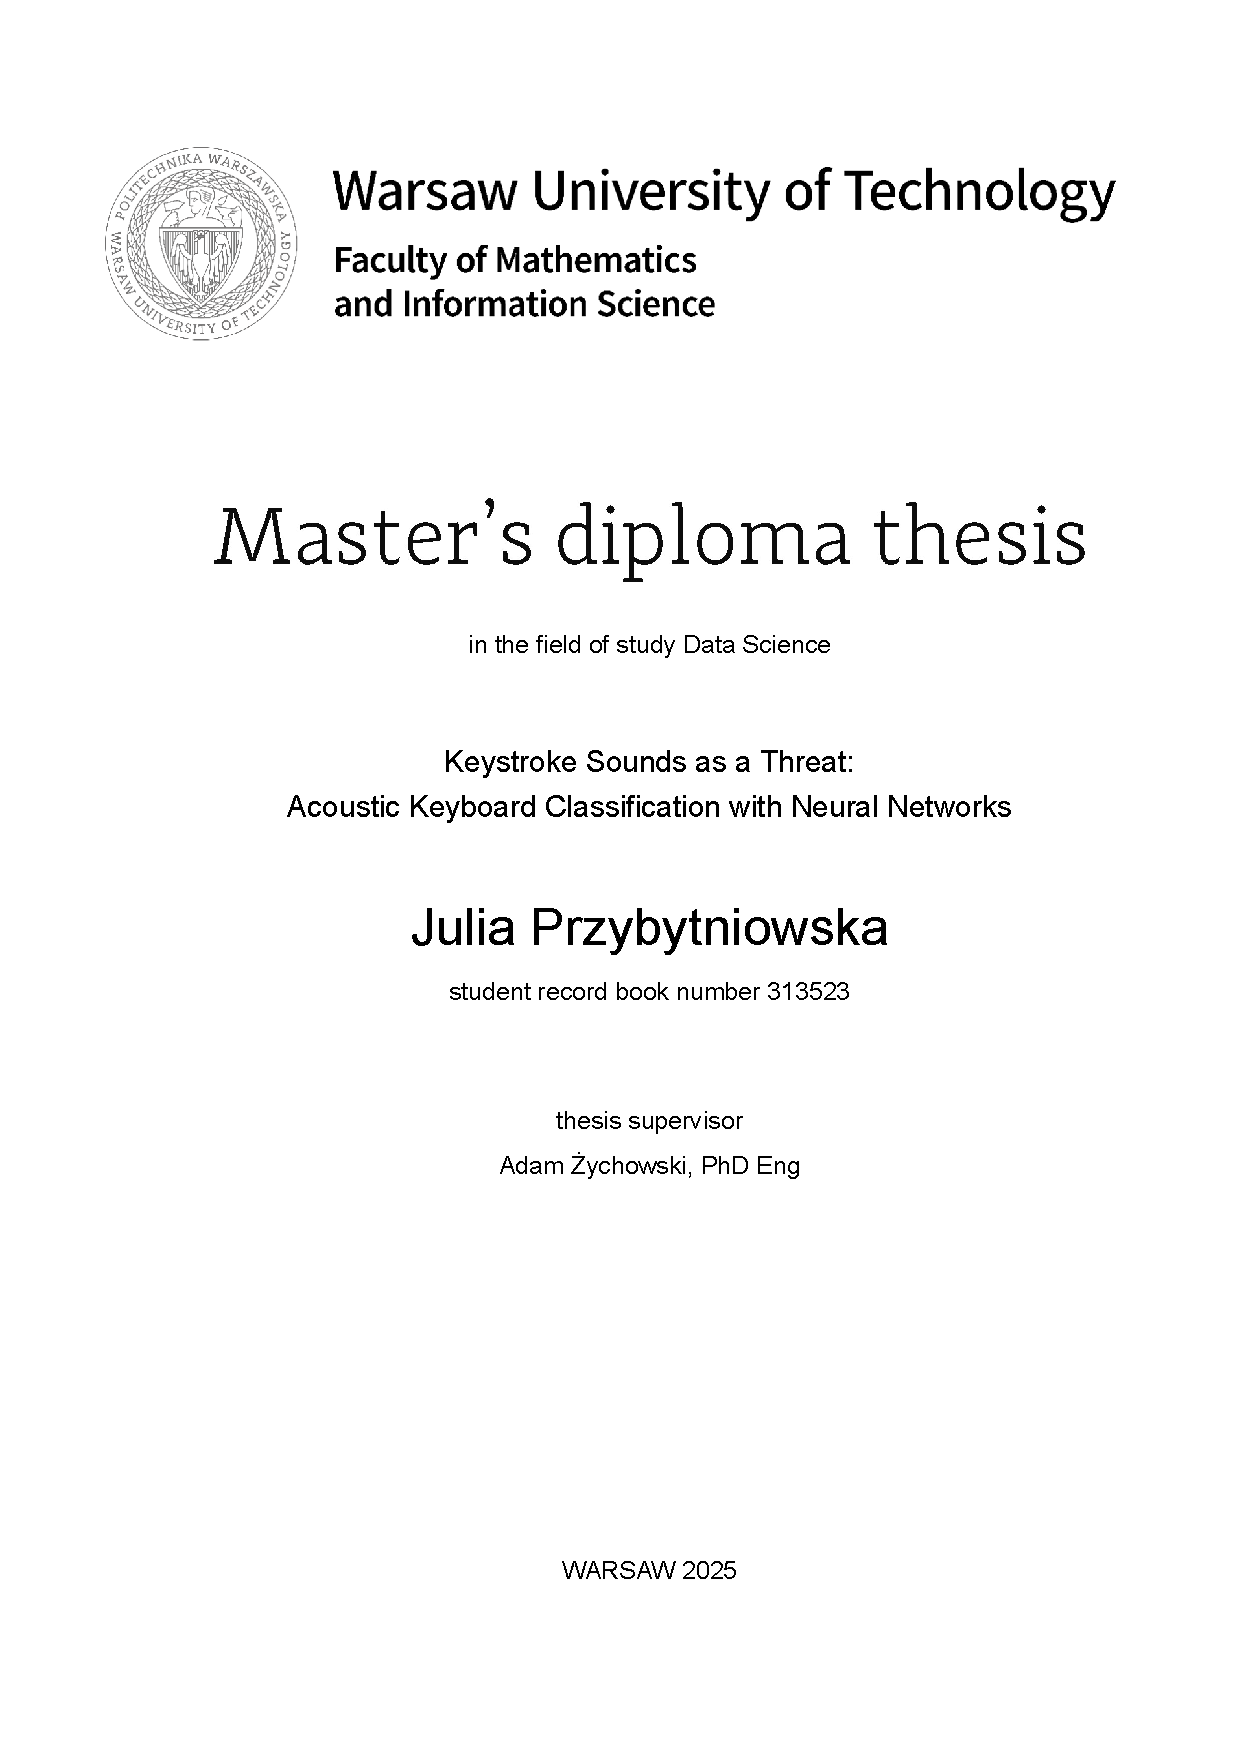
\includepdf[pages=-]{./title_page/titlepage-msc-en}

\null\thispagestyle{empty}\newpage

% ------------------ PAGE WITH SIGNATURES --------------------------------

%\thispagestyle{empty}\newpage
%\null
%
%\vfill
%
%\begin{center}
%\begin{tabular}[t]{ccc}
%............................................. & \hspace*{100pt} & .............................................\\
%supervisor's signature & \hspace*{100pt} & author's signature
%\end{tabular}
%\end{center}
%


% ---------------------------- ABSTRACTS -----------------------------

{  \fontsize{12}{14} \selectfont
\begin{abstract}

\begin{center}
\title
\end{center}

\noindent \textbf{Keywords:} acoustic side-channel attacks, convolution, attention, neural networks, keystroke recognition, data privacy, machine learning

In the pursuit of stronger digital security, research has largely focused on encryption, biometrics, and hardened systems. Yet devices still emit subtle traces, side channels, that attackers can exploit, with keystroke sounds posing a particularly concerning risk.

This thesis evaluates a range of neural network architectures for acoustic keystroke recognition across different environments, background conditions, and key sets. The models achieved 92\% accuracy on publicly available recordings and set a new state-of-the-art performance on existing benchmarks.

Beyond accuracy, the work investigates how training data, model scale, and noise exposure affect generalization, and explores whether large language models can use semantics to repair errors in raw predictions. The study highlights both the possibilities and limits of acoustic side-channel attacks, pointing to effective defense strategies such as noise injection, hardware modifications, or keyboard design.

\end{abstract}
}

\null\thispagestyle{empty}\newpage


{\selectlanguage{polish} \fontsize{12}{14}\selectfont
\begin{abstract}

\begin{center}
\tytul
\end{center}


\noindent \textbf{S\l{}owa kluczowe:} akustyczne ataki bocznokana\l{}owe, konwolucja, mechanizmy uwagi, sieci neuronowe, rozpoznawanie naci\'sni\k{e}\' c klawiszy, prywatno\'s\'c danych, uczenie maszynowe

W d\k{a}\.zeniu do wzmocnienia bezpiecze\'nstwa cyfrowego badania koncentruj\k{a} si\k{e} g\l{}\'ownie na szyfrowaniu, biometrii i odpornych systemach. Urz\k{a}dzenia wci\k{a}\.z jednak emituj\k{a} subtelne sygna\l{}y, kana\l{}y boczne, kt\'ore mog\k{a} zosta\'c wykorzystane przez atakuj\k{a}cych, a d\' zwi\k{e}ki naci\'sni\k{e}{\' c} klawiszy stanowi\k{a} w tym kontek\'scie szczeg\'olnie powa\.zne zagro\.zenie.

Niniejsza praca analizuje r\'o\.zne architektury sieci neuronowych do rozpoznawania naci\'sni\k{e}\' c klawiszy na podstawie sygna\l{}\'ow akustycznych, w zr\'o\.znicowanych \'srodowiskach, warunkach t\l{}a oraz zestawach klawiszy. Opracowane modele osi\k{a}gn\k{e}\l{}y dok\l{}adno\'s\'c na poziomie 92\% w przypadku og\'olnodost\k{e}pnych nagra\'n i ustanowi\l{}y najwy{\. z}szy wynik (state-of-the-art) na istniej\k{a}cym benchmarku.

Poza sam\k{a} dok\l{}adno\'sci\k{a}, badania koncentruj\k{a} si\k{e} na wp\l{}ywie danych treningowych, skali modeli i ekspozycji na szumy na zdolno\'s\'c uog\'olniania, a tak\.ze sprawdzaj\k{a}, czy du\.ze modele j\k{e}zykowe mog\k{a} wykorzystywa\'c kontekst semantyczny do naprawiania b\l{\k e}d\'ow w surowych predykcjach. Praca wskazuje zar\'owno na mo\.zliwo\'sci, jak i ograniczenia akustycznych atak\'ow bocznokana\l{}owych, a tak\.ze sugeruje skuteczne strategie obrony, takie jak unikanie przebywania w ciszy, modyfikacje sprz\k{e}towe czy zmiany w konstrukcji klawiatur.

\end{abstract}
}

\null\thispagestyle{empty}\newpage

\section*{The use of IT tools in this thesis}
\vspace{3pt}

\normalsize
% In the case of multiple authors, please change to "We" below
I hereby declare that:
\begin{enumerate}
    \item I have used IT tools to generate the content of the manuscript of this thesis.
    \item I have not used IT tools to generate the code of the software developed for the thesis.
    \item I take full responsibility for all content in this thesis, including both the manuscript and the software developed for it.
\end{enumerate}

\begin{table}[h]
\centering
\begin{tabular}{|p{0.5\textwidth}|p{0.5\textwidth}|}
\hline
\textbf{The scope of the use of IT tools to generate manuscript} & \textbf{The scope of the use of IT tools to generate software code} \\ \hline
AI tools were used to improve the style of the text and to assist in gathering several thoughts into one.
& Not Applicable                       \\ \hline
\end{tabular}
\end{table}

\null\thispagestyle{empty}\newpage
%% --------------------------- DECLARATIONS ------------------------------------
%
%%
%%	IT IS NECESSARY OT ATTACH FILLED-OUT AUTORSHIP DEECLRATION. SCAN (IN PDF FORMAT) NEEDS TO BE PLACED IN scans FOLDER AND IT SHOULD BE CALLED, FOR EXAMPLE, DECLARATION_OF_AUTORSHIP.PDF. IF THE FILENAME OR FILEPATH IS DIFFERENT, THE FILEPATH IN THE NEXT COMMAND HAS TO BE ADJUSTED ACCORDINGLY.
%%
%%	command attacging the declarations of autorship
%%
%\includepdf[pages=-]{scans/declaration-of-autorship}
%\null\thispagestyle{empty}\newpage
%
%% optional declaration
%%
%%	command attaching the declaataration on granting a license
%%
%\includepdf[pages=-]{scans/declaration-on-granting-a-license}
%%
%%	.tex corresponding to the above PDF files are present in the 3. declarations folder
%
\null\thispagestyle{empty}\newpage
% ------------------- TABLE OF CONTENTS ---------------------
% \selectlanguage{english} - for English
\pagenumbering{gobble}
\tableofcontents
\thispagestyle{empty}
\newpage % IF YOU HAVE EVEN QUANTITY OD PAGES OF TOC, THEN REMOVE IT OR ADD \null\newpage FOR DOUBLE BLANK PAGE BEFORE INTRODUCTION


% -------------------- THE BODY OF THE THESIS --------------------------------

% \null\thispagestyle{empty}\newpage
\pagestyle{fancy}
\pagenumbering{arabic}
\setcounter{page}{11}


\chapter{Introduction}

As technological developments continue to focus on strengthening device security through advanced encryption algorithms (\textit{\cite{encryption}}, \textit{\cite{imageencryption}}), biometric authentication (\textit{\cite{biometric1}}, \textit{\cite{biometric2}}) and robust system designs (\textit{\cite{securesystem}}), an often neglected vulnerability is side-channels - unintentional leaks of information that attackers can exploit. Unlike traditional attack methods, side-channel attacks do not rely on breaking encryption or bypassing system controls, but instead exploit data, such as electromagnetic signals, power consumption or acoustic emissions, which seem harmless on their own. However, in-depth analysis of these unintentional signals can allow the collection of sensitive data.

Among its various forms, acoustic side-channel attacks are particularly tricky because they exploit sounds generated by a device or its components, such as keyboard strokes, and can bypass even the most carefully designed systems. For example, consider entering your PIN at an ATM while other people are waiting in line in a relatively quiet environment. Among those waiting, there may be an attacker who will record the subtle sounds of keystrokes to reconstruct the PIN. Similarly, during an online meeting, when a user is multitasking and typing confidential information at the same time, all the person on the other side of the computer has to do is press record of the meeting. In this way, one is able to capture the sounds of keystrokes and decrypt the data being entered.

The danger of these attacks lies in their ability to indirectly compromise secure systems. A user entering a password may take measures to protect the screen from prying eyes, but not pay attention to the beeps as they type. Such oversight opens the way for attackers armed with modern tools such as machine learning algorithms and neural networks. Using advanced techniques, attackers can analyze subtle acoustic signatures from keystrokes, often imperceptible to human ears, to reconstruct sensitive information. Each keystroke generates a unique sound (\textit{\cite{uniquekeys}}) due to the physics of the keyboard creating a specific acoustic signature for each key, allowing them to be identified with a degree of certainty.

Side-channel attacks, including acoustic variants, are not a new phenomenon. Already in 1956, during the Suez Crisis, the UK Security Service infiltrated the Egyptian embassy in London and discreetly modified its telephone system. This allowed them to eavesdrop on the sounds of a clerk inputting the day’s key settings into a cipher machine. This historical case highlights how even seemingly minor vulnerabilities can be exploited to extract highly sensitive information, underscoring the enduring threat posed by side-channel attacks.

This study explores the potential of acoustic side-channel attacks on keyboards, leveraging machine learning techniques to better understand and address these threats. Specifically, the research described in this document focuses on developing a state-of-the-art solution for an audio classification task that targets distinct keyboard keystroke sounds. The main goal is to design a model capable of accurately predicting typed text based on these sounds, using advanced neural network architectures to decode keystroke patterns from audio data.

To accomplish this, a comprehensive dataset needs to be created that includes different typing styles, different keyboards, and recordings performed in different acoustic environments. This comprehensive data set ensures that the model can generalize well across a wide range of real-world scenarios, increasing the robustness of the analysis.

However, in addition to achieving high prediction accuracy, this work also aims to explore methods that interfere with the model and limit its performance. Therefore, why focus on building a model capable of extracting these sounds only to find ways to counteract it? The answer lies in the principle of knowing your enemy. By thoroughly understanding how these attacks operate and identifying their strengths and weaknesses, we are more capable of developing an effective defense. Having a full understanding of the threat allows us to design targeted countermeasures, raising awareness and increasing the security of sensitive information against such loopholes.




\chapter{Related Work}

Based on the concerns outlined in the introduction, it is necessary to delve into existing research, particularly the one targeting keyboard keystroke recognition. The main goal of these studies was to assess the precision and feasibility of such attacks, highlighting weaknesses present even in well-designed systems. By studying how accurately sensitive information can be reconstructed from acoustic signals, the researchers discovered critical factors that contribute to the success of such attacks. These factors include the characteristics of the physical structure of the keyboard, the acoustic environment in which the data is recorded, and the methods used to process and analyze the captured signals.

Many studies highlight how subtle differences in sound frequency, amplitude and time provide a wealth of information about individual keystrokes. Such analyses also highlight the limitations of human perception compared to the capabilities of computational methods in decrypting acoustic signals. Using advanced tools such as machine learning models and signal processing techniques, researchers have shown that even seemingly negligible acoustic emissions can carry enough information to compromise sensitive data.

Approaches to analyzing acoustic side-channel attacks can be broadly divided into three categories: time-based, geometry-based and frequency-based methods. Each of these specific angles offers unique insights into how keystroke information can be extracted from acoustic signals and provides crucial insights into the strengths and limitations of different analytic strategies. The following subsections delve into these categories, exploring how they contribute to a broader understanding of acoustic side-channel sensitivity. A comprehensive comparison of these and additional approaches can be found in a detailed survey of side-channel attacks and defenses by \textit{\cite{2023survey}}.

\section{Time-based analysis}

The time-based approach to acoustic lateral attacks focuses on analyzing temporal patterns in keystroke activity. Timing information, such as the time a key is pressed (hold time), the interval between pressing and releasing a key (release time), and the time between successive key presses, provides attackers with valuable insight into typing behavior. By exploiting these subtle temporal fluctuations, attackers can infer the sequence of keys pressed and reconstruct them with some confidence.

A noteworthy study by \textit{\cite{timebased}} demonstrates the feasibility of user-independent timing attacks on PINs using advanced metrics for precise analysis. The research proposes constructing a dictionary of the time between keystrokes, including all possible PINs and their corresponding timing sequences. These sequences were derived from a cognitive model simulating typical user behavior. After capturing the time sequence between the victim's keystrokes, the attacker uses metrics such as cosine similarity and cross-correlation to compare the observed sequence with entries in the dictionary.
The combination of metrics used contributes significantly to the success of the work, as cosine similarity measures the angular distance between time vectors, identifying patterns even when the absolute durations differ slightly. On the other hand, cross-correlation shifts signals to align peaks, effectively detecting matches despite temporal noise. The attack has achieved remarkable success rates, recovering the correct PIN within the first three guesses 75\% of the time and within the first 10 guesses 80\% of the time.

While these results underscore the effectiveness of timing-based analysis, the reliance on precise similarity metrics also introduces challenges in broader real-world applications. For instance, noisy environments, inconsistent typing behaviors, or sequences extending beyond short PINs can reduce the attack's accuracy. Despite its limitations, the study highlights how sophisticated metric-based approaches can extract significant information from subtle timing variations.

\section{Geometry-based analysis}

Geometry-based approaches to acoustic side-channel attacks use the physical placement of keys on a keyboard to identify which key was pressed. These techniques are based on measuring differences in the time it takes for sound waves to reach two or more microphones. Using methods such as Time Difference of Arrival (TDoA), or Differential Audio Analysis (DAA), attackers can estimate the physical location of the keys pressed, regardless of the type or meaning of the text entered. This makes geometry-based approaches comprehensive, as they can be used to recover random text, such as passwords or PIN codes, with high accuracy.

One notable application of geometry-based techniques is the Time Difference of Arrival (TDoA) approach, utilised by \textit{\cite{tdoa}}, where a smartphone and its two build-in microphones were used to capture acoustic emanations from keystrokes.
The approach uses geometric principles to estimate the set of possible key positions on a plane, and the results show the system's ability to recover up to 94\% of keystrokes with just one phone and keyboard. Accuracy was highly dependent on the position of the phone, but the method showed promising results in controlled environments.

However, the TDoA method can be applied using multiple microphones. In such cases, acoustic signals collected from different microphones are used together to narrow down the set of candidate key positions, thereby reducing the dependence of the prediction on the position from which the sounds are captured. \textit{\cite{tdoa2}} utilized more than two microphones for this experiment, and acquired a success rate of more than 86\%. However, the dependence on multiple recording devices also makes the approach somewhat impractical in real-world scenarios where attackers may not have access to such resources.

Another geometry-based approach is Differential Audio Analysis, implemented by \textit{\cite{daa}}. The method leverages two microphones built into the device to capture audio and has achieved 98\% accuracy on older cell phones with physical keyboards, demonstrating the potential of geometry-based techniques when the right hardware is available. However, these methods make crucial assumptions about the number and arrangement of devices, as well as the size and layout of the keys. In practice, achieving the high performance metrics described in these studies would require carefully controlled conditions that are not always feasible in real-world attacks.

While geometry-based approaches, particularly TDoA and DAA, have shown impressive results in laboratory settings, their reliance on multiple microphones, specific device configurations and precise placement limits their use in everyday scenarios. Nonetheless, these techniques highlight the potential for highly accurate keystroke recovery when the necessary conditions are met and could, in combination with other more general methods, provide high predictions.

\section{Frequency-based analysis}

The third method for analyzing sound is a frequency-based approach that focuses on analyzing the spectral properties of sound signals to extract meaningful information. Unlike time-domain analysis, which looks at how the signal varies over time, the frequency-based approach examines how the signal’s energy is distributed across various frequencies. This shift to the frequency domain reveals valuable insights into the sound's structure that are often not immediately obvious in the time domain, especially in applications like acoustic side-channel attacks, speech recognition, and audio classification.

To begin the process of frequency-based analysis, the signal is typically transformed from the time domain to the frequency domain using a mathematical tool known as the Fast Fourier Transform (FFT), explained by \textit{\cite{fft}}. FFT is a powerful algorithm that decomposes a signal in the time domain into its constituent frequencies, revealing how much energy is present in each frequency component. Once the signal is transformed, it is often split into overlapping windows to capture the evolving spectral content over time.

\begin{figure}[h!]
    \centering
    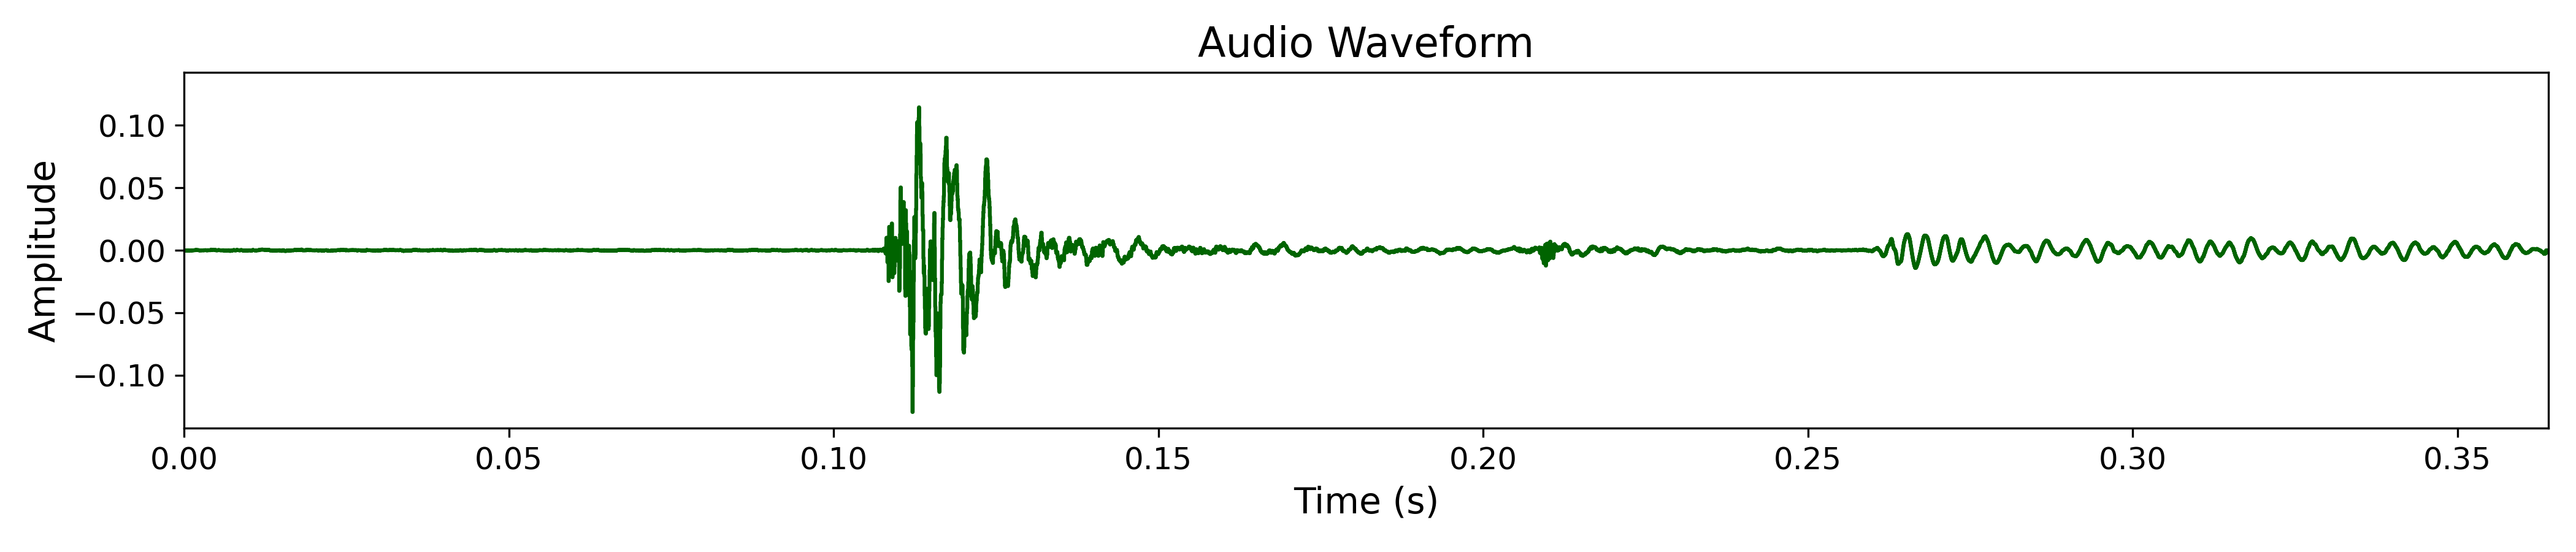
\includegraphics[width=0.9\linewidth]{img_related_work/waveform.png}
    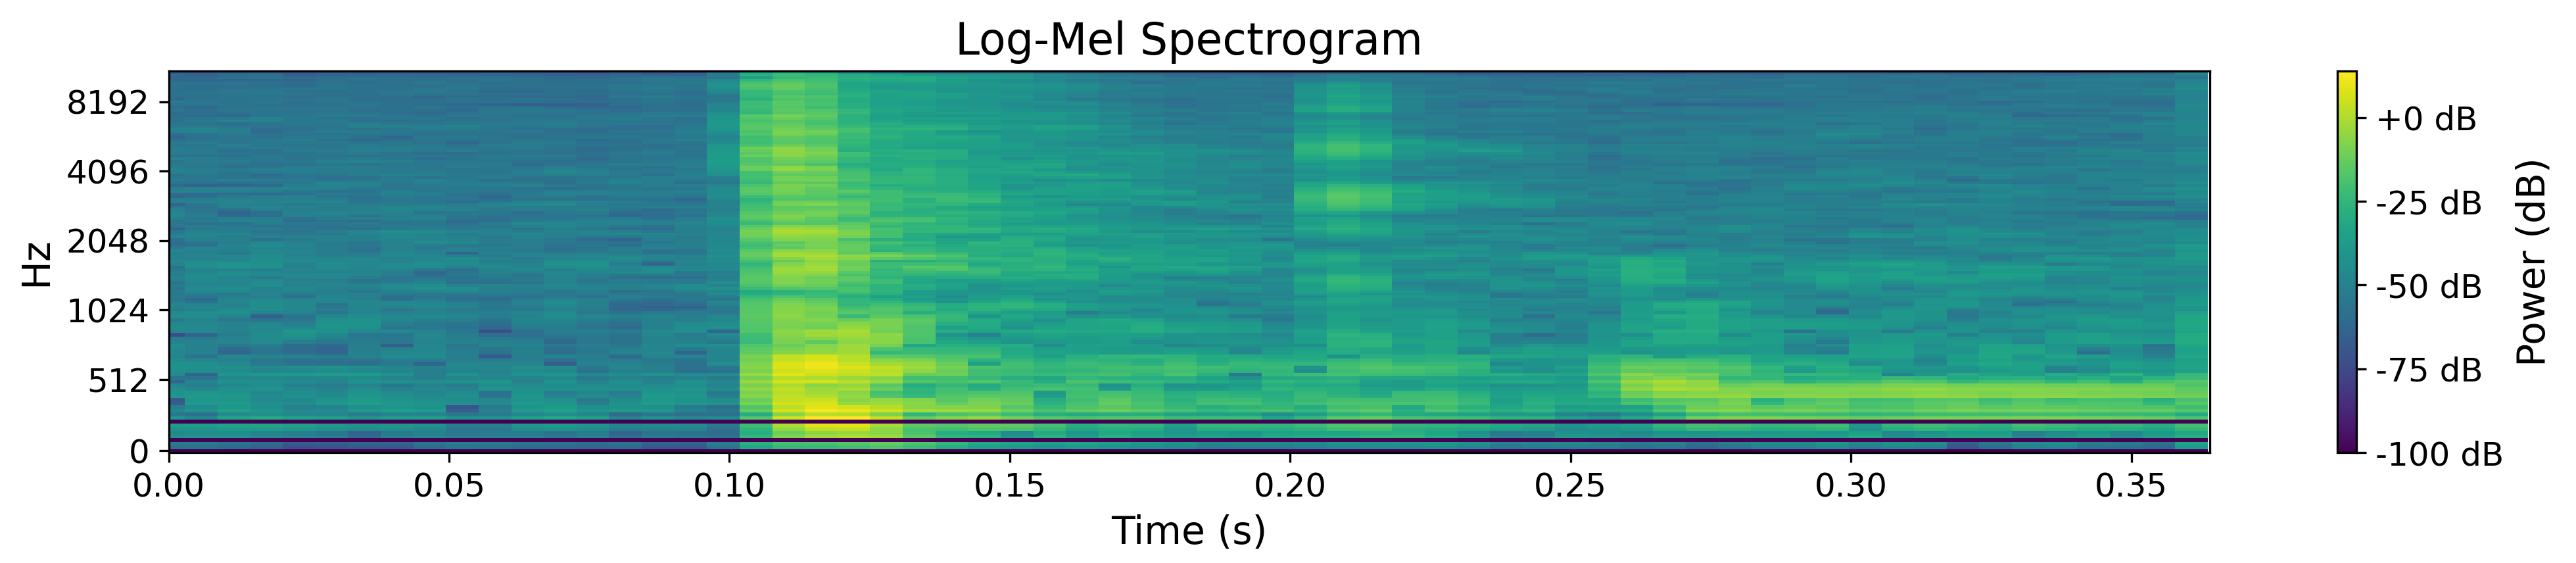
\includegraphics[width=0.9\linewidth]{img_related_work/log_mel_spectrogram.png}
    \caption{An example of log-mel spectrogram for a given key press.}
    \label{fig:spectogram}
\end{figure}

After transforming a signal into the frequency domain, researchers often proceed to generate a spectrogram, a visual representation of the signal's frequency content over time. On a spectrogram, presented in Figure \ref{fig:spectogram}, the horizontal axis represents time, the vertical axis represents frequency, and the intensity or color of each point on the graph represents the amplitude or strength of a specific frequency at a particular time. The spectrogram allows us to track how frequencies evolve over time, providing insight into transient events. For more precise analysis, a mel-spectrogram is often used. The mel spectrogram is a refined version of the traditional spectrogram that uses a mel scale designed to mimic the frequency sensitivity of human hearing. The mel scale compresses higher frequencies and expands lower frequencies to better match the way people perceive sound, making it often more effective. To streamline the analysis, researchers typically extract features such as Mel-Frequency Cepstral Coefficients (MFCC) from the mel-spectrogram. This process involves logarithmically transforming the signal's power spectrum to compress a range of values, then applying a discrete cosine transform (DCT) to reduce the number of coefficients while retaining the most important features. These coefficients provide a compact representation of the signal's frequency content and are immune to background noise, making them particularly suitable for tasks in noisy environments.

Depending on the approach taken, solutions can be generally divided into two groups: those that use classical machine learning techniques and those that utilize deep learning architectures.

\section*{Classical Machine Learning approach}

In classical machine learning methods, researchers typically extract features, such as FTT or MFCC coefficients, which serve as input for traditional classifiers such as support vector machines (SVMs), random forests or k-nearest neighbors (KNNs). These methods rely on manual feature extraction and selection, followed by the application of machine learning algorithms to recognize patterns in the data.

However, deep learning methods have gained popularity because of their ability to automatically learn feature representations directly from raw audio data. Recurrent Neural Networks (RNNs), introduced by \textit{\cite{rnn1}} and \textit{\cite{rnn2}}, are often used for sequential data processing, making them effective at capturing temporal dependencies in audio signals. These networks excel at modeling the evolution of features over time, which is essential for tasks such as speech recognition and side-channel acoustic attacks.

Alternatively, when audio data is converted to a visual format, such as a spectrogram or mel-spectrogram, the problem becomes an image classification task. This allows the use of convolutional neural networks (CNNs) (\textit{\cite{cnn}}), or vision transformers (\textit{\cite{vit}}), which are proficient at extracting both temporal and spectral features, so that their combinations are often considered the best solutions in this area.

Frequency-based methods have proven to be a successful solution against acoustic side-channel attacks, making it possible to extract sensitive information from subtle sound patterns. The following pages present and describe key studies that expose the application and effectiveness of these methods in real-world scenarios.\\


A notable example of successful application using classical machine learning methods is the work titled "Don’t Skype \& Type! Acoustic Eavesdropping in Voice-Over-IP" by \textit{\cite{skypetype}}.

This study presents an advanced attack methodology capable of inferring sensitive keystroke information transmitted during Voice over IP calls, such as those enabled through the Skype platform. Focusing on real-world scenarios in which the attacker is present during a meeting or online conversation, the authors proved the possible effectiveness of side-channel attacks even under bandwidth constraints and speech overlap, in an uncontrolled environment.

\begin{figure}[h!]
    \centering
    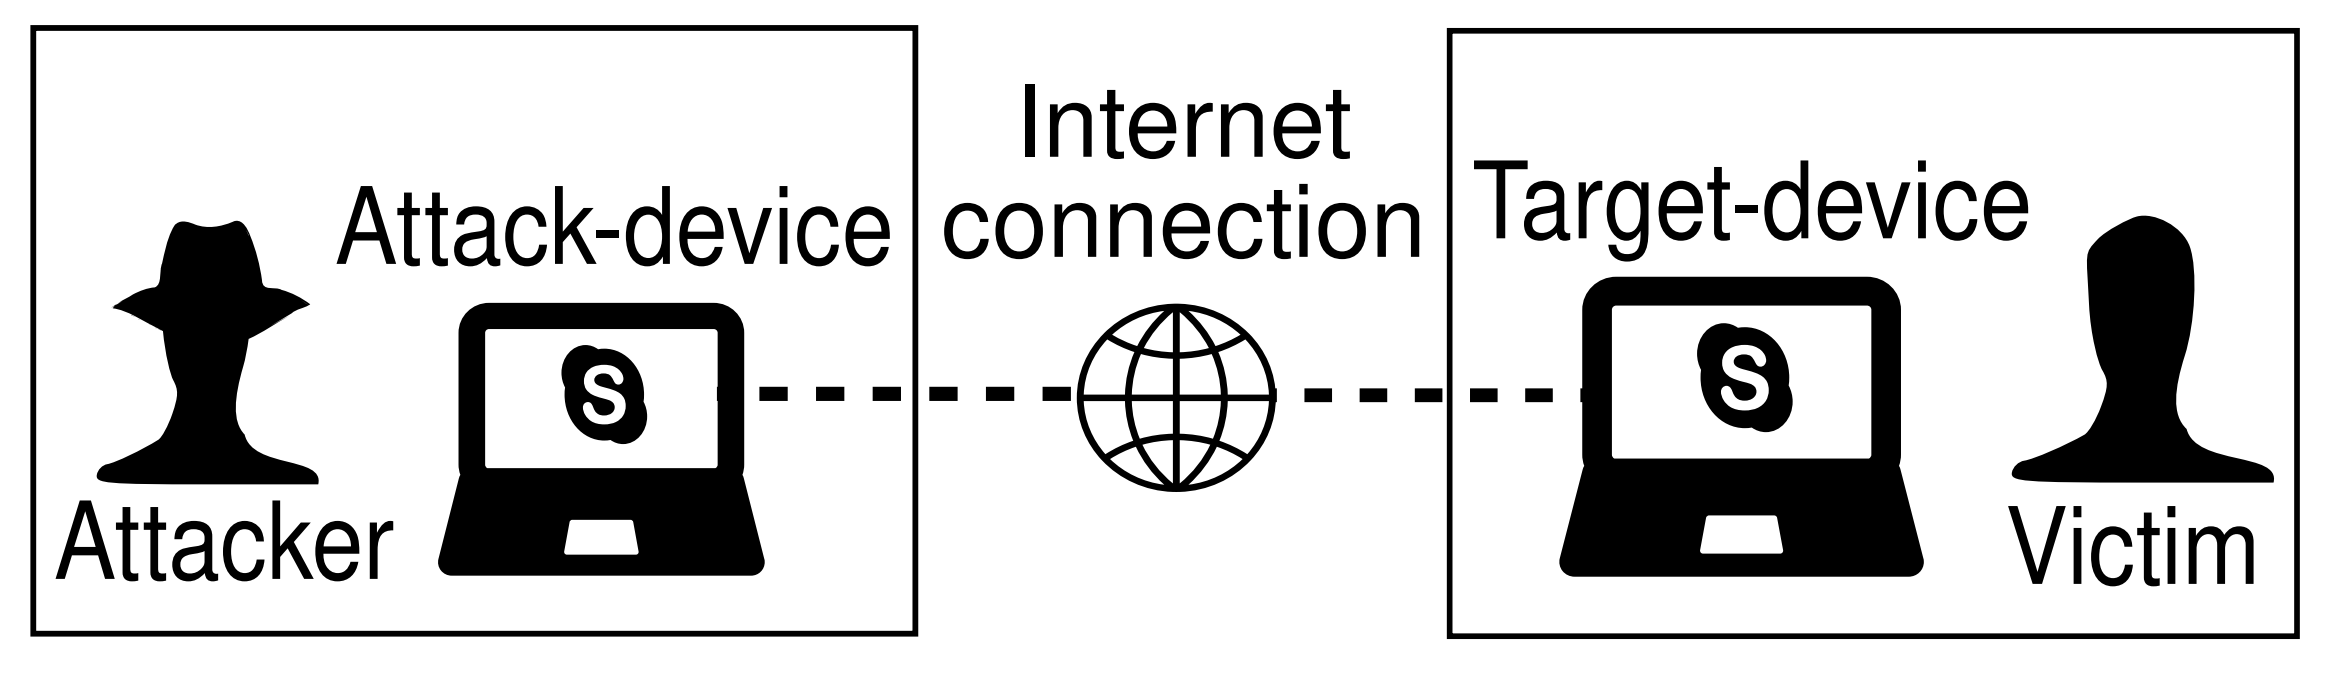
\includegraphics[width=0.6\textwidth]{img_related_work/skype_arch.png}
    \caption{The architecture of the proposed system for keystroke inference during VoIP calls.}
    \footnotesize{Sourced from original paper \cite{skypetype}.}
    \label{fig:skypetype}
\end{figure}

\noindent The attack's foundation rests on the definition of three distinct scenarios: \\
\texttt{Complete Profiling:} The attacker has access to the exact keyboard and typing style of the victim. \\
\texttt{User Profiling:} The attacker knows the device victim has but is not aware of the typing style.\\
\texttt{Model Profiling:} The attacker has no prior knowledge of the victim’s device or typing style.\\

The data processing pipeline in this research emphasizes isolating individual keystroke sounds to extract features for classification. Each keystroke sound typically exhibits two distinct peaks in its waveform, as shown in Figure \ref{fig:skypewaveform}. The authors use the peak of the keystroke, which is much louder and clearer, to detect and separate the sounds, while the peak of the release is ignored due to its lower amplitude.

\begin{figure}[h!]
  \centering
  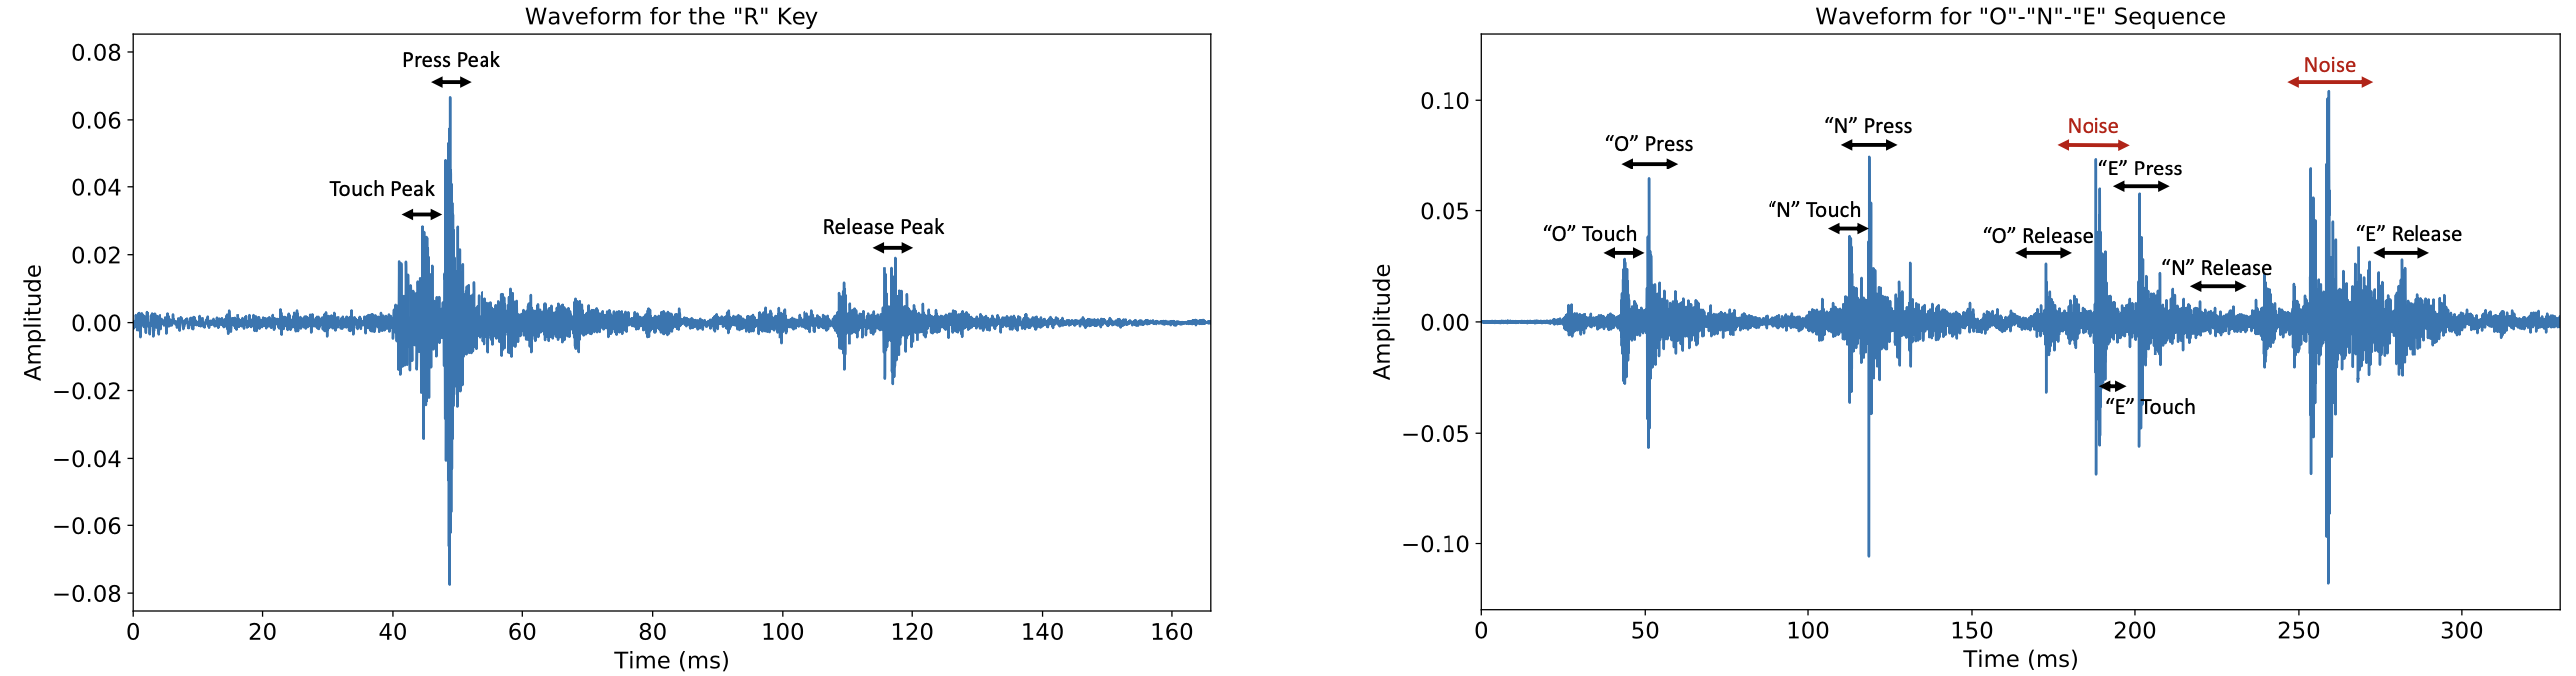
\includegraphics[width=\textwidth]{img_related_work/release_peak.png}
  \caption{Waveform of a keystroke sound, showing two distinct peaks.}
  \footnotesize{Sourced from work by \cite{rnn2019}.}
  \label{fig:skypewaveform}
\end{figure}

To automatically detect and isolate keystrokes, the authors normalized the amplitude of the audio signal to obtain a Root Mean Square value of 1, ensuring consistent scaling. The energy for each 10ms window of the signal was calculated by summing its Fast Fourier Transform (FFT) coefficients and used for keystroke detection. The event was identified when the energy in a given window exceeded a configurable threshold, which was adjusted based on training data to optimize detection accuracy.

Once a keystroke event was detected, a wavelength segment of 100 ms or shorter was extracted, if possible, and passed on for classification. This method effectively distinguishes between individual keystrokes, focusing on the louder peaks of the keystroke, However, by using this method, the authors significantly reduced the expected search space, ignoring the possibility of entering a string of special characters.

Several spectral features were taken into experiments to acquire the most informative and compact audio features. That includes FFT coefficients, cepstral coefficients, and Mel-Frequency Cepstral Coefficients (MFCC), where the last method was ultimately selected as it consistently outperformed other features.

Once the features are extracted, the next phase of the methodology focuses on classification. In the device profiling scenario, the study uses a k-nearest neighbor (k-NN) classifier, where k is set to 10, to predict the type of keyboard used by the victim based on the extracted features. The approach aims to match the victim's keyboard with the keyboard contained in the set of known keystroke hits. To classify keystrokes, the study evaluated several machine learning algorithms, including logistic regression, linear discriminant analysis (LDA), support vector machines (SVM) and random forests (RF). Among these classifiers, using 10-fold cross-validation, each consisting of 10 probes of each of 26 a-z keys, logistic regression outperformed the others in the precision, after an extensive grid search. Classification performance is measured using top-1 and top-$k$ accuracy rates, denoting the percentage of cases in which the true class appears in the first n predictions of the fitted model.

The results of the classification experiments show that the attack methodology is highly effective across the different attack scenarios. In the Complete Profiling scenario, where the attacker has access to detailed information about the victim’s device and typing style, the accuracy of keystroke classification is notably high. Even in the more challenging Model Profiling scenario, where the attacker has no prior knowledge of the victim’s device or typing style, the methodology achieves a substantial improvement over random guessing, with top-1 accuracy increasing by up to 312\%. These results highlight the danger of the attack success, even when the attacker has limited access to computational resources. \\

One year later \textit{\cite{anand2018keyboard}} presented a similar study, focusing on detecting random passwords and PIN codes with noisy background. The authors utilized classical machine learning methods to classify alphanumeric keystrokes (a-z and 0-9), aiming to identify the most effective feature extraction techniques and machine learning algorithms. To achieve this, they evaluated performance using 10-fold cross-validation on a dataset using following algorithms: Simple Logistic Regression, Multinomial Logistic Regression, J48, Random Forest, SMO and Linear Nearest Neighbor Search, with results summarized in Figure \ref{fig:anand2018}.

\begin{figure}[h!]
    \centering
    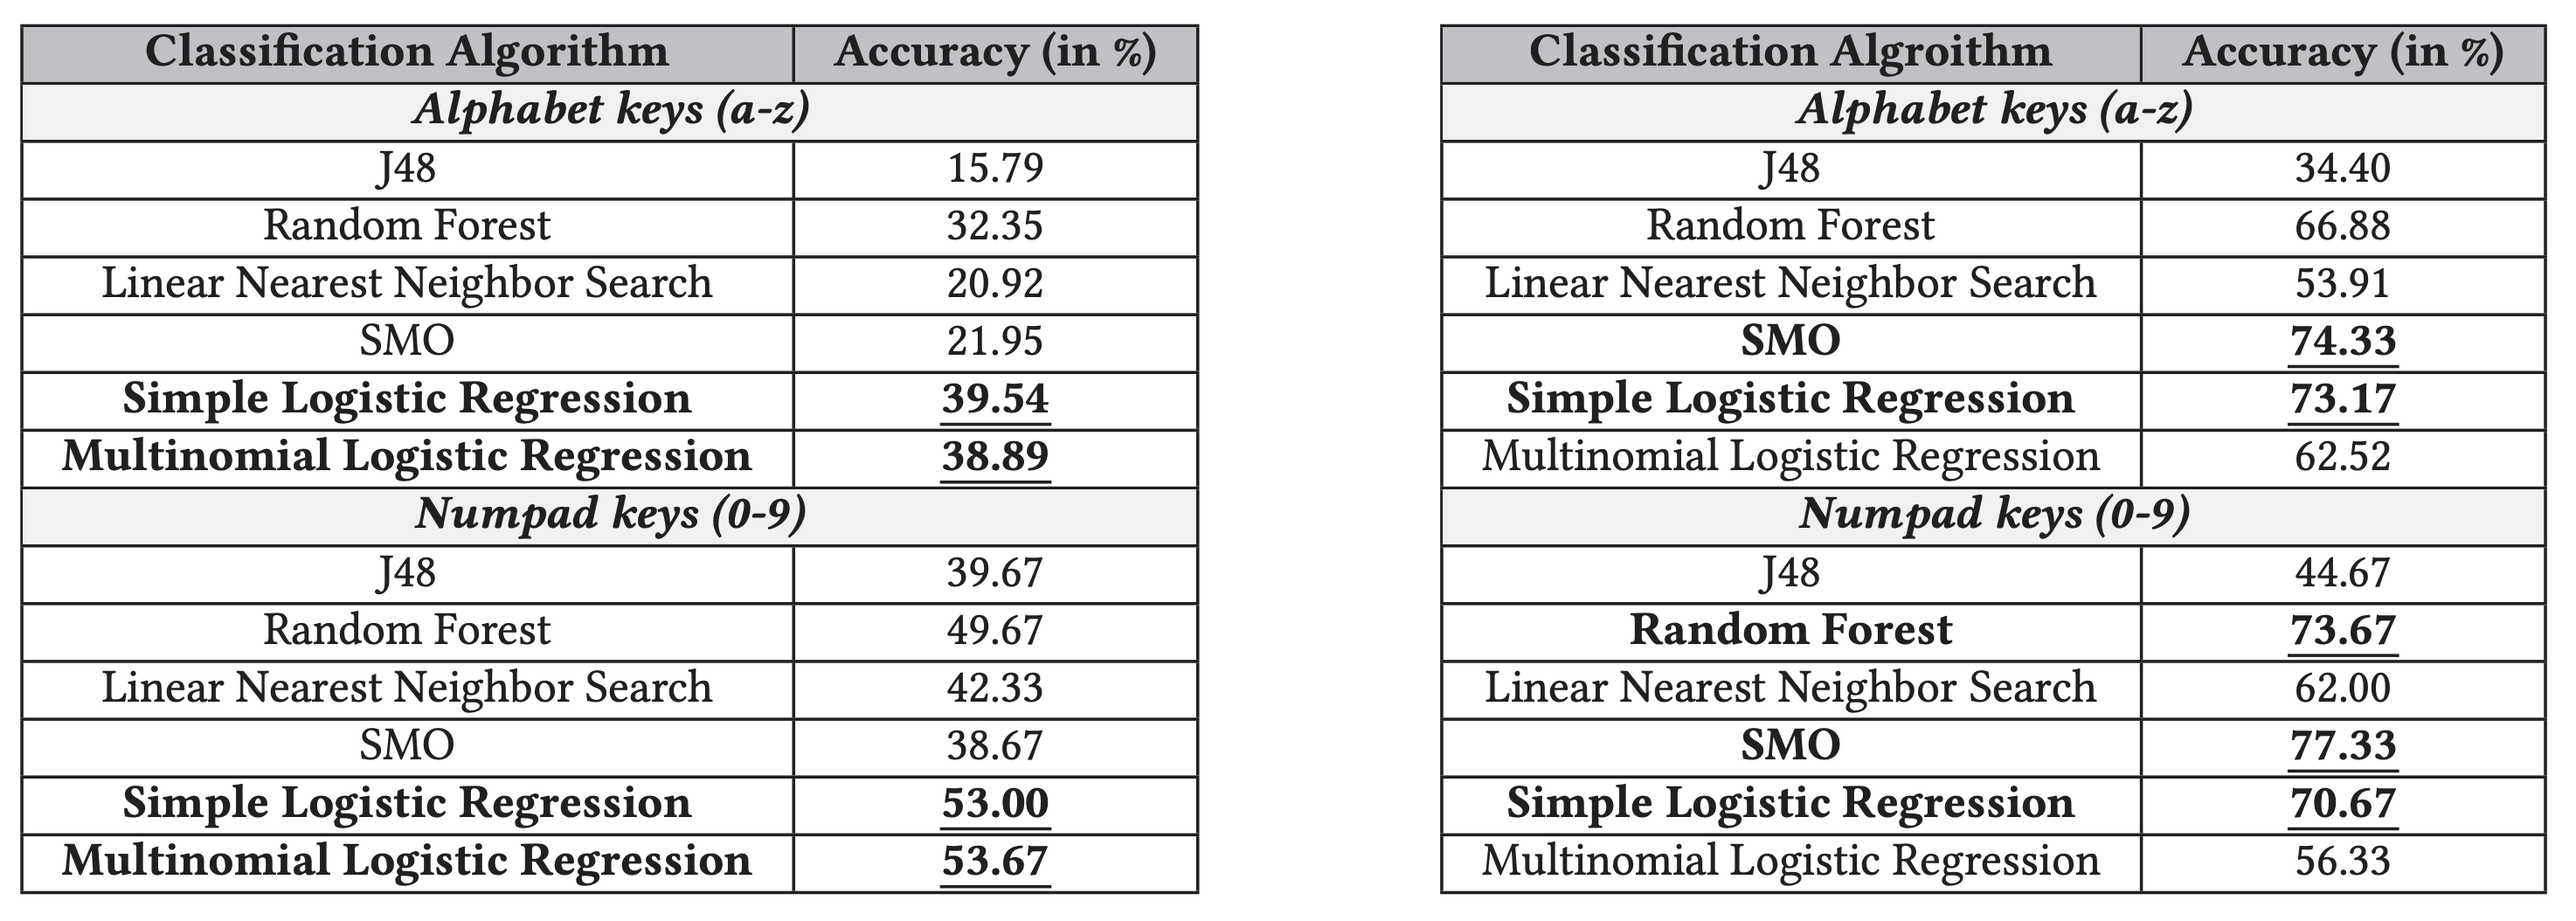
\includegraphics[width=0.9\textwidth]{img_related_work/fft_vs_mfcc.png}
    \caption{Comparison of classification accuracy across different machine learning algorithms: FFT coefficients (left) and MFCC features (right).}
    \footnotesize{Sourced from original paper \cite{anand2018keyboard}.}
    \label{fig:anand2018}
\end{figure}

It's strongly visible that the MFCC provide a better set of features, enriching a classification accuracy, than FFT coefficients.

The second goal of their work was to investigate the effect of different types of background noise on the performance of keystroke classification models, testing white noise and false keystroke methods. White noise is a random signal with a constant spectral density and infinite bandwidth, but in this experiment it was limited to the frequency range of keystroke sounds. False keystrokes, on the other hand, are pre-recorded keystroke sounds played continuously without gaps between keystrokes. Discoveries have shown that background noise suppression in most microphones and voice calling software, including Skype, makes white noise an ineffective method of masking keystrokes and thwarting eavesdropping attacks. Additionally, while Skype did not filter out fake keystrokes, they were more effective at masking keystroke sounds compared to white noise. The study also noted that speech, when present in a conversation, was less effective than false keystrokes, but more effective than white noise in reducing attack accuracy. \\

\section*{Deep Learning approach}

Given scenarios in which an attacker has access to large computational resources and can train deep neural network-based architectures, the question arises: Can they successfully infer what is being typed and in what way?

A study titled 'Keyboard Snooping from Mobile Phone Arrays with Mixed Convolutional and Recurrent Neural Networks' by \textit{\cite{cnn2019noise}} explores this assumption, showing that deep learning algorithms can produce better results than classical methods.

Researchers have developed a system that uses several smartphones to detect keyboard keystrokes by capturing acoustic signals. This innovative approach involved placing multiple mobile phones around a table, each equipped with built-in microphones and motion sensors, recording both the sound of the keys being pressed and the associated vibrations. Participants were instructed to type naturally while talking, introducing a significant amount of noise to collect data and making the experiment strongly resemble real-world conditions. As a result, in the data collected, more than 40\% of keystrokes occurred while participants were talking, making them much more difficult to recognize.

To process the collected raw signals, the researchers used a segmentation technique that divided the audio data into overlapping windows, each 100 ms long with a step of 25 ms. This ensured efficient management of the continuous signal and provided labeled windows corresponding to specific keys pressed, or a special marker for windows with no keys pressed. In cases where multiple keys were pressed in a single window, the label was assigned to the first key detected. Integrating Fast Fourier Transform (FFT) and Mel-Frequency Cepstral Coefficients (MFCC) with raw audio and motion data, the researchers used a multimodal architecture to improve detection performance.

Actual typing behavior often results in an unbalanced data set because some keys are used much more often than others. For example, the space bar is pressed hundreds of times more often than keys such as “z” or “q”. Unlike other studies that artificially balanced their datasets by forcing participants to type the same key repeatedly, this study retained the natural imbalance to better reflect realistic typing scenarios. To address the issue of rare keys, the researchers grouped some keystrokes into broader categories. For example, all punctuation marks were combined into one class, as were all numbers and both Alt keys, creating 34 classes.

The researchers divided the problem into two components: keystroke detection, aimed at predicting whether any key was pressed in a given signal frame, and keystroke classification, focused on determining which specific key was clicked. Detection was essential to this architecture because of their approach to data processing, which included signal windows that did not contain keystrokes. A 5-fold cross-validation was used for the detection task, prioritizing true-positive and true-negative indicators over accuracy to better reflect the practical application of the model.

The system employed a multi-modal architecture that could take any combination of four feature types as input: FFT coefficients, MFCC, raw audio, and raw motion data, presented in Figure \ref{fig:cnn2019-label}. Using convolutional neural networks (CNNs), the researchers processed the extracted audio features, raw audio, and motion data. Each input type passed through a unique convolutional architecture comprising a mix of one-dimensional convolutional layers, max pooling layers, and residual blocks. After passing through the convolutional layers, the outputs were flattened into one-dimensional arrays, concatenated, and fed into dense layers for final processing.


\begin{figure}[h!]
  \centering
  \begin{minipage}{0.575\linewidth}
      \centering
      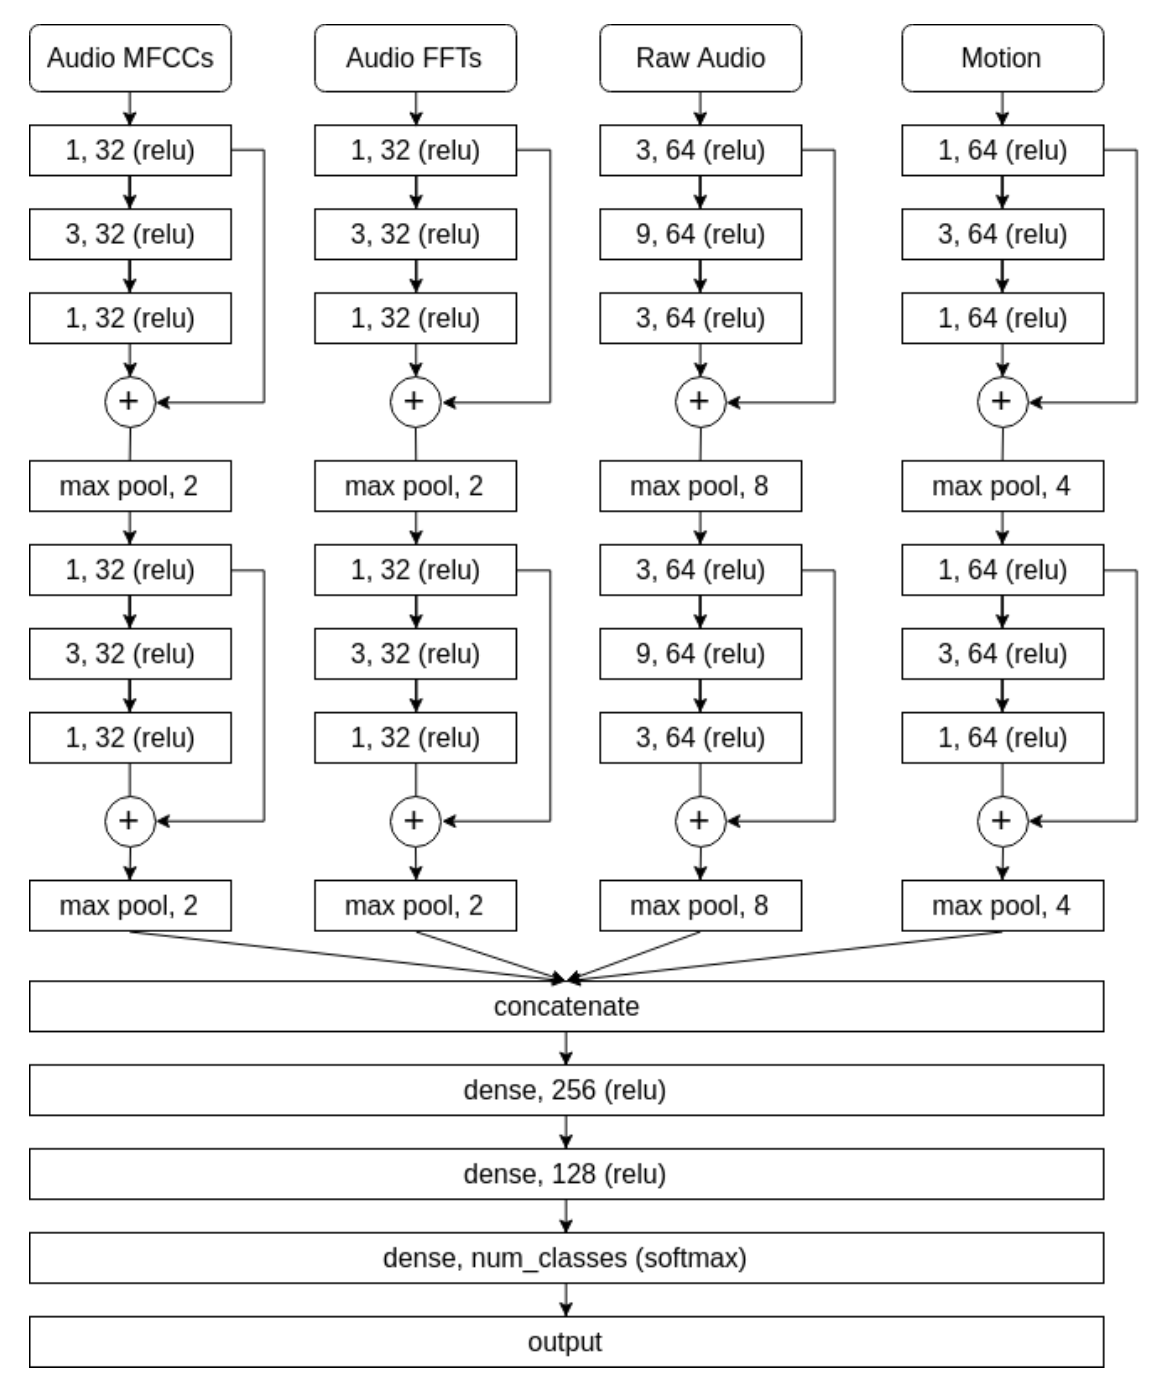
\includegraphics[width=\linewidth]{img_related_work/cnn2019.png}
      \subcaption{Keystroke detection architecture.}
      \label{fig:cnn2019-label}
  \end{minipage}
  \hfill
  \begin{minipage}{0.41\linewidth}
      \centering
      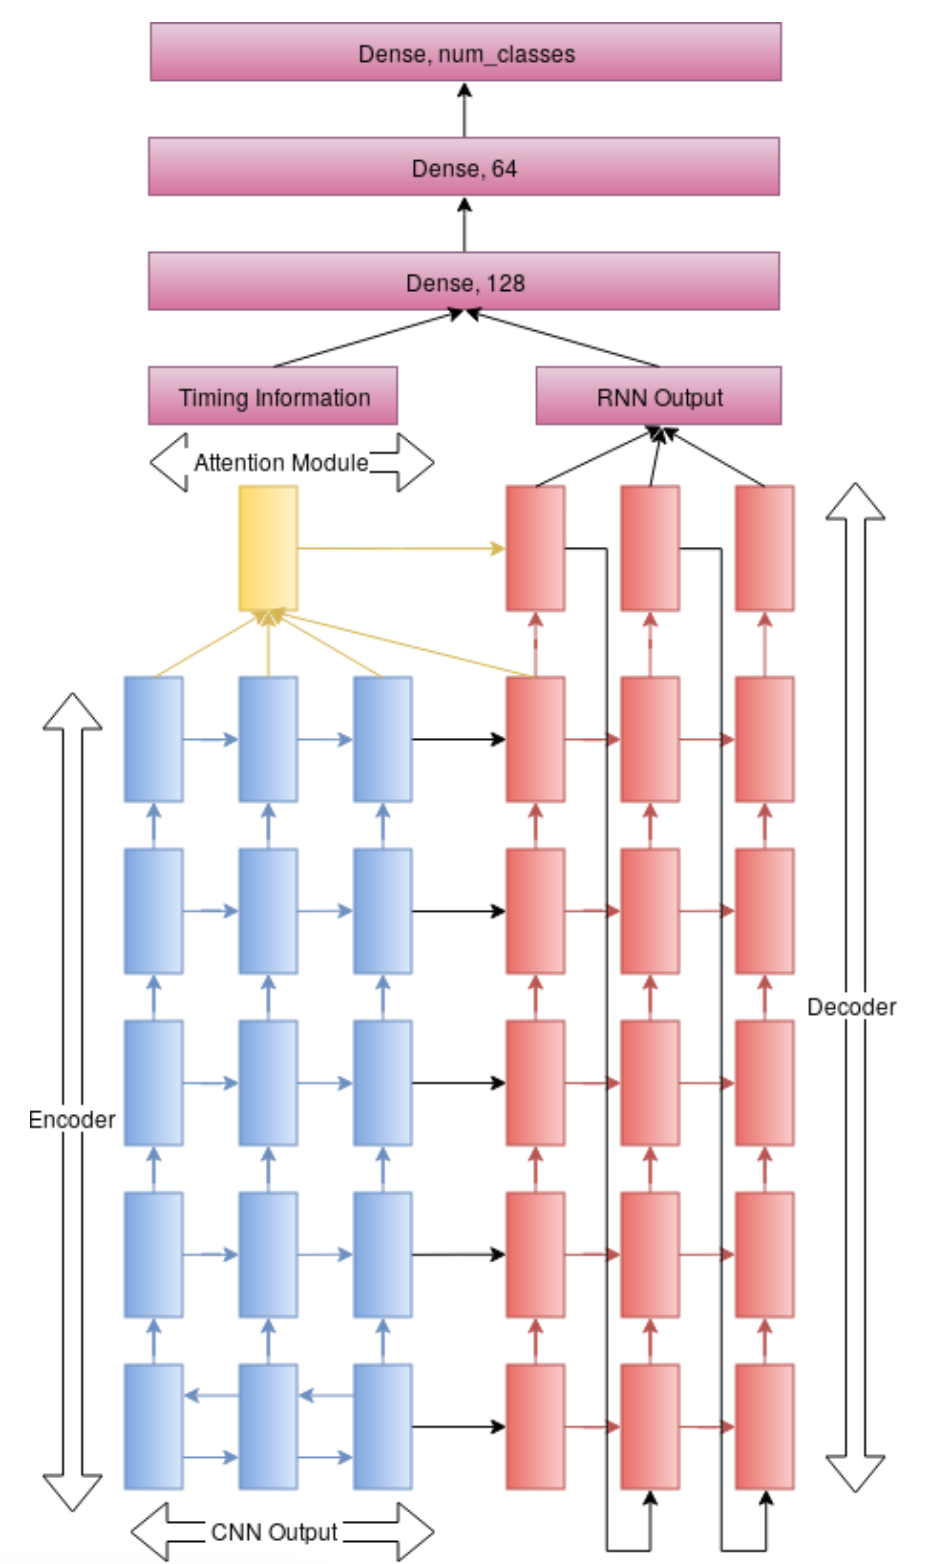
\includegraphics[width=\linewidth]{img_related_work/rnn2019.png}
      \subcaption{Classification architecture.}
      \label{fig:rnn2019-label}
  \end{minipage}
  \caption{Schemas of the keystroke detection and classification architectures.}
  \footnotesize{Sourced from original paper \cite{cnn2019noise}.}
  \label{fig:enter-label}
\end{figure}

For the keystroke classification component, the researchers implemented a recurrent neural network (RNN)-based classification model to correct systematic errors made by the CNN, shown in Figure \ref{fig:rnn2019-label}. The authors noted that the CNN component frequently exhibited three key types of errors: it confused infrequent keystrokes with frequent classes, misclassified characters that were physically close on the keyboard, and keys that were physically similar in size (e.g., backspace and enter). These patterns suggested that the CNN was primarily learning a physical model of keystroke dynamics. To address these systematic errors and misspellings, the researchers used an architecture inspired by Google's Neural Machine Translation (NMT) model \cite{nmt}, effectively defining the task as a translation problem.

The RNN architecture consisted of three main components: an encoder, a decoder and an attention module, in which each block of the architecture used LSTM (Long Short-Term Memory) cells, introduced by \cite{lstm}. The encoder contained five LSTM layers, while the decoder consisted of six LSTM layers. The bottom layer of the encoder was a bidirectional LSTM, allowing the model to use a right-to-left hierarchy in the input data. In addition, the residual connections between the LSTM layers facilitated the training of both shallow and deep layers, allowing deeper architectures to be created without compromising learning performance.

During training, the CNN output was passed to the encoder, while the decoder received the ground truth keystrokes. At inference time, the decoder was instead initialized with a special start token and generated the sequence step by step, using its previous output as input, until a stop signal was produced. This iterative process resembled sequence-to-sequence translation tasks.

In the keystroke detection task, the results showed the effectiveness of combining various input features for model performance. Including FFT coefficients, MFCC, raw audio data and raw motion data, the model achieved a true positive performance rate of 85\% and a true negative performance rate of 75\%. It's worth noting that when the model relied solely on motion data, the rates were 2\% higher. However, the researchers noted that the detection model introduced an inherent error of about 12.5\%, which was also factored into the classification of the sounds.

For the keystroke classification task, system performance varied depending on the type of input data and architecture. Top-1 and Top-5 character accuracy ranged from 16.2\% and 43.7\% to 26.3\% and 55.\%, with the highest performance achieved using MFCC input data. Integrating RNN with CNN, especially when combined with MFCC features, significantly improved performance, with the model achieving 41.8\% for Top-1 accuracy and 70.6\% for Top-5 accuracy. These results highlight the significant predictive power added by RNN, underscoring its important role in improving classification accuracy.

In supplementary research, the authors examined how different environmental factors affected the model's performance. Changing the room in which participants typed had a noticeable effect on accuracy, but not a detrimental one, due to differences in acoustical characteristics of the room. Changing the tabletop material significantly affected accuracy, with the metal tabletop performing worse than the composite artificial wood. Finally, the model had difficulty generalizing to the new laptop keyboard and encountered significant difficulties with the ergonomic keyboard, highlighting the challenges of adapting to different typing surfaces.\\


Not long after the previous study was published, another paper used a deep learning model combining CNNs and RNNs, although with some minor differences. The research conducted by \textit{\cite{rnn2019}} described a system that introduced a novel approach, particularly noteworthy because of the data set collected.

The researchers collected data from a total of 17 users, fluent in English and well-acquainted with programming languages. The data collection included six tasks, created as a Cartesian product of (English, coding) and (fixed text, variable text and free text). Each user performed about 4-5 randomly assigned tasks, resulting in about 30 minutes of recorded audio per participant, creating a final dataset consisting of 86,000 keystrokes.

For pre-processing, the study followed previous work that identified a reasonable frequency range for keystroke spectra, using low-pass and high-pass filters to preserve frequencies between [1000, 16000] Hz. However, the data still contained unsteady noise, such as the sounds of moving coffee cups, coughing or conversation. To effectively deal with short times between keys, the researchers used a 40 ms window for segmentation, finding that it was better than longer windows that are often chosen in the literature. In addition, they moved the window 10 ms ahead of the detected bin to capture the peak of the touch, which also significantly improved classification performance. It is worth noting that most keystrokes segmented in this way did not include a release peak, so even if shift key was predicted, the attacker would not know for how long characters were capitalized.

The evaluation used two metrics: character error rate (CER) and accuracy. CER, specifically based on Levenshtein distances, calculated the minimum number of insertions, substitutions and deletions required to transform a predicted result into a reference transcript normalized by the reference length. Accuracy was used for direct comparisons with other solutions, which is quite difficult due to the differing characteristics of the experiments. Interestingly, while previous work suggested that MFCC were the most efficient method for feature extraction, this study found that the FFT transformation provided better performance in their dataset.

The architecture used in this study was adapted from the literature on speech recognition \cite{speech2016}, designed as a complex system to predict keystroke sequences directly from the input audio, which schema is presented in Figure \ref{fig:speech2016arch}.

\begin{figure}[h!]
    \centering
    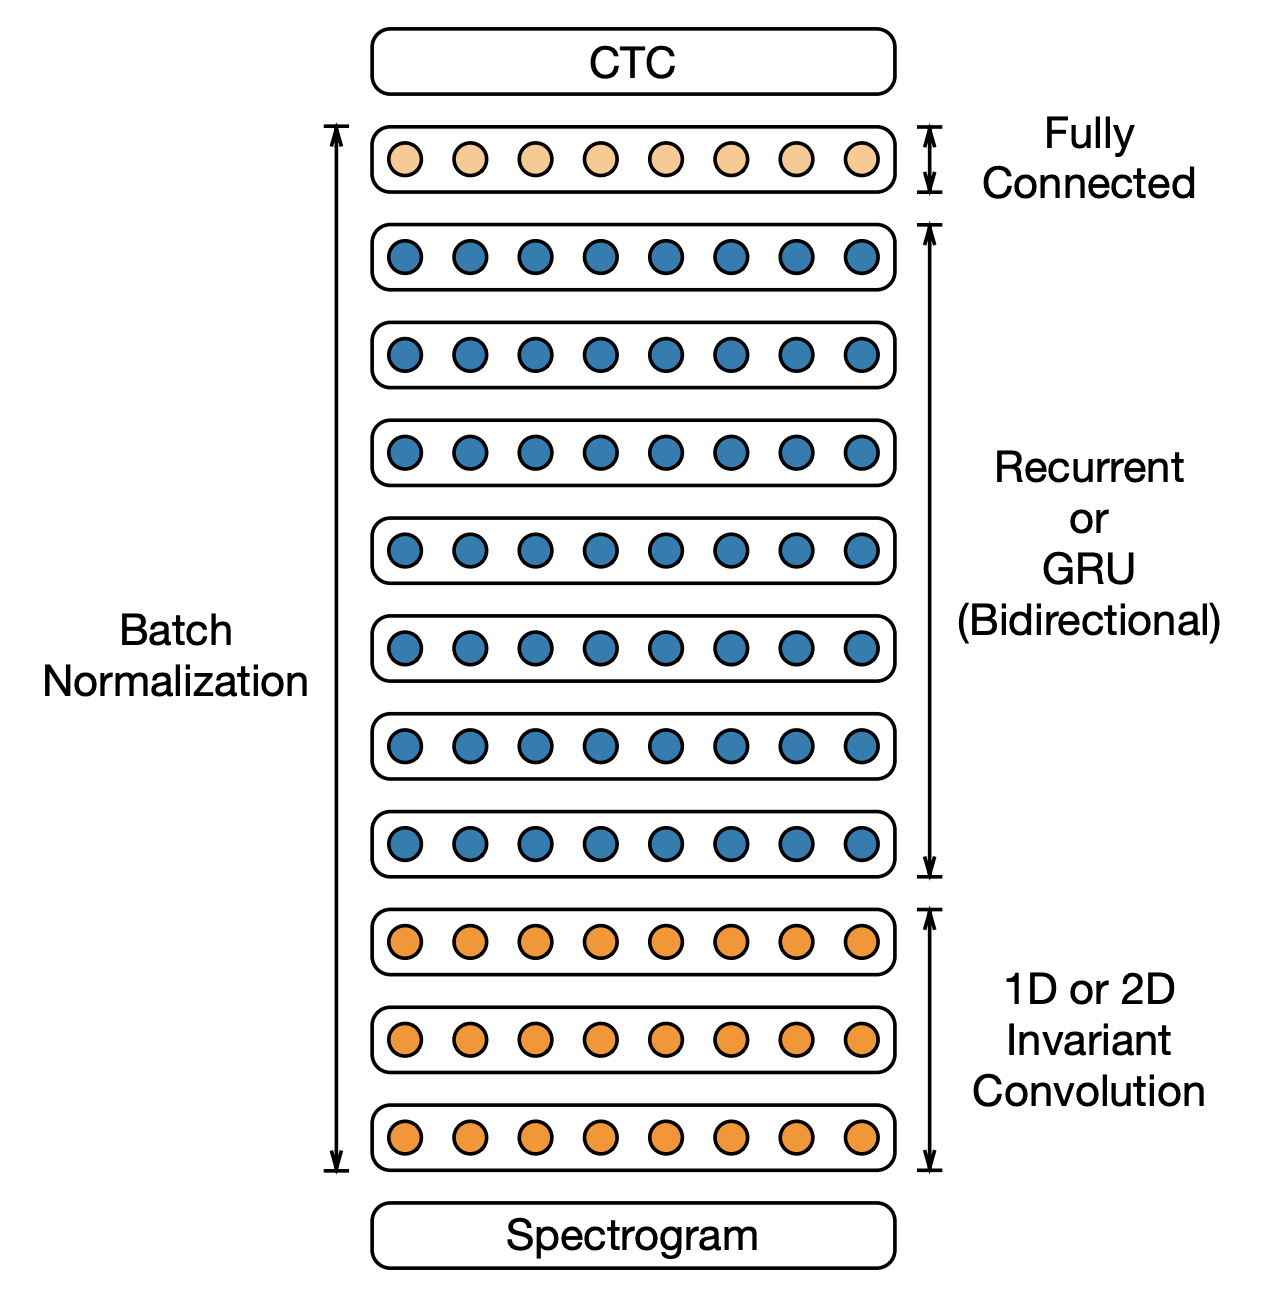
\includegraphics[width=0.5\textwidth]{img_related_work/speech2019arch.png}
    \caption{The architecture of speech recognition system.}
    \footnotesize{Sourced from original paper \cite{speech2016}.}
    \label{fig:speech2016arch}
\end{figure}

For acoustic processing during training, each writing session was divided into 20-second waveforms sampled at 16 kHz. The spectra were normalized for the training data, and then augmentation was applied to them, changing the tempo of each recording randomly disturbed by $\pm15\%$ and amplified by $\pm6\%$.

The implemented deep learning architecture consisted of five layers: two 2D convolutional layers with batch normalization (\textit{\cite{batchnorm}}), followed by two bidirectional RNN layers and one fully connected layer for keystroke label prediction. The initial CNN layers performed convolutions in both time and frequency domains using 32 filters with a kernel size of $41\times11$ and a step size of $2\times2$. After the convolution layers, two bidirectional GRU (Gated Recurrent Unit presented by \textit{\cite{gru}}) layers with 800 nodes each were used to capture sequential dependencies in the data. The architecture was trained using both the cross entropy and CTC loss, with the CTC function providing much more stable convergence during training.

The results showed a significant improvement over the baseline model from \textit{\cite{skypetype}} when evaluated using the Character Error Rate (CER). For English typing, the RNN model achieved a CER of 7.41\%, compared to 36.0\% for the baseline, while for coding the CER was reduced from 33.2\% to 11.14\%. Even when typists were excluded from the training set and included only in the test set, the RNN model maintained a relatively low CER of 15.41\% for English and 20.13\% for coding, compared to baseline results ranging between 38\% and 41\%. The results underscore the characterization of RNN and their ability to perform serial analysis, with little reduction in their precision on the analysis of a previously unknown typing style.\\



Following previously described work that applied CNNs with residual blocks and attention mechanisms to keystroke classification, another innovative study by \textit{\cite{2023convmixer}} applied advanced architectures to a different but related problem. This study focused on recognizing the sounds associated with typing specific passwords, shifting the goal from generalized keystroke classification to predicting a limited set of the 15 most popular passwords based on acoustic signals. Unlike zero-shot or few-shot learning, which involves generalizing to all possible keystroke combinations, this task required identifying predefined classes of passwords.

In this research, each password was recorded 30 times, thus yielding a collection of 450 audio files of passwords. These recordings were then processed by converting each audio waveform into a spectrogram, with extracted features by utilizing MFCC.

Although convolutional neural networks (CNNs) have long been the standard for computer vision tasks, the authors noted a shift in recent studies favoring transformer-based models such as Vision Transformer (ViT) (\textit{\cite{vit}}), ConvMixer (\textit{\cite{convmixer}}) and MLP-Mixer (\textit{\cite{mlpMixer}}), which have been shown to outperform traditional CNN architectures such as ResNet (\textit{\cite{resnet}}) and VGG (\textit{\cite{vgg}}). Since ConvMixer showed better performance in similar problems compared to ViT, as well as MLP-Mixer, this one was chosen as the basis for their research.

ConvMixer combines elements of vision transformers and MLP mixers, relying solely on convolutional operations for feature extraction. The architecture, presented in Figure \ref{fig:convmixer}, begins with a patch embedding process that divides the input spectrogram into smaller patches, embedding them into feature tokens. This step transforms the $N \times N$ image into a feature map of size $h \times n/p \times n/p$, where $h$ represents the hidden dimension and $p \times p$ represent the patch size. After this embedding, a GeLU activation layer and a batch normalization layer are applied to standardize and prepare the data for deeper layers.

\begin{figure}[h!]
    \centering
    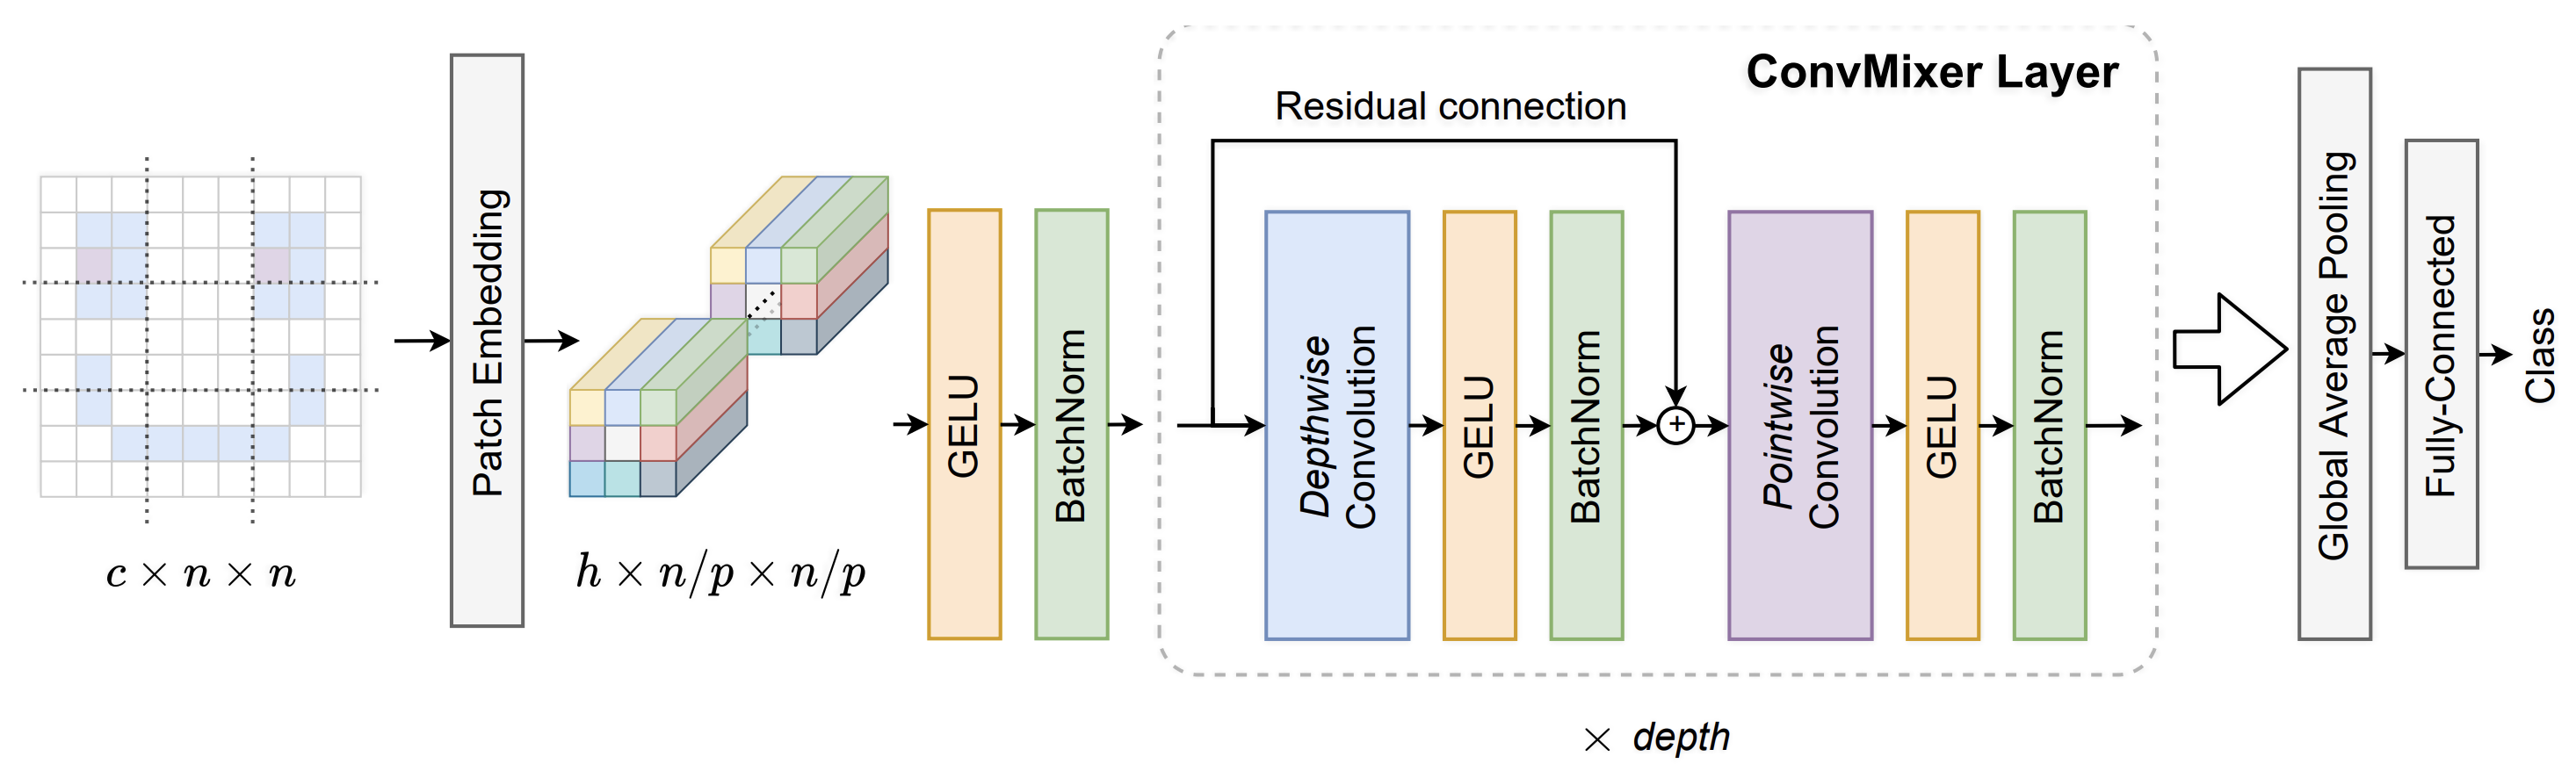
\includegraphics[width=\textwidth]{img_related_work/convmixer.png}
    \caption{The ConvMixer architecture for password classification.}
    \footnotesize{Sourced from original paper \cite{2023convmixer}.}
    \label{fig:convmixer}
\end{figure}

The core of ConvMixer is the main layer, which consists of a residual block containing a depth splicing operation. This block integrates the output of one layer with the depth splicing from the next, allowing the model to retain important features while improving computational efficiency. Depth convolution is followed by Pointwise Convolution and additional activation blocks, allowing the network to efficiently separate and analyze information. This sequence is repeated across multiple layers, gradually creating a hierarchical representation of spectrogram features.

The final stage of the ConvMixer architecture includes a global pooling layer, which reduces the dimensionality of the extracted features into a fixed-size vector. This vector is subsequently passed to a softmax classifier or another task-specific head for the classification task. Despite its conceptual similarities to vision transformers, ConvMixer achieves competitive performance while relying entirely on standard convolutional operations, offering a streamlined yet powerful approach for password classification based on acoustic spectrograms.

With this architecture in place, the researchers trained the ConvMixer model on the password dataset, using hold-out cross-validation to ensure robust evaluation. The dataset was divided into a 90\% training set and a 10\% test set, and the classification process was repeated ten times to compute the average accuracy, reducing the variability introduced by random data partitioning.

ConvMixer was trained using the Adam optimizer (first presented by \textit{\cite{adamopt}}), with a maximum of 70 epochs and an initial learning rate of 0.01. The training process took only 8 minutes and 21 seconds, and the test accuracy achieved was 91.11\%. As the data contains only 30 samples of each class, the augmentation strategy was adopted, that involved resizing, rotation, translation, and reflection operations. The input images were randomly translated by up to three pixels both horizontally and vertically and were rotated, leading to accuracy ranging from 97.78\% to 88.89\%, with an average of 92.44\%.

In addition, the researchers conducted experiments tuning the VGG16 and ResNet18 models on the same data set. Tuning ResNet18 resulted in an average accuracy of 88.35\%, while tuning VGG16 achieved a slightly lower average accuracy of 85.92\%. Thus, ConvMixer definitely outperformed CNN-only based architectures in this classification problem. \\


Last but not least, a study closely related to research conducted in this thesis is titled “A Practical Deep Learning-Based Acoustic Side Channel Attack on Keyboards” by \textit{\cite{CoAtNet2023}}. The work introduces a novel technique for implementing deep learning models with layers of self-attention to perform acoustic side channel attacks. The study focused on 36 laptop keyboard keys (covering the digits 0-9 and the letters a-z) and started with a single recording of each key pressed 25 times in a row. The authors developed a function to isolate individual keystrokes from these recordings, which, despite the challenges of the recordings made by Zoom, was able to determine an effective threshold for segmenting keystrokes.

The authors again used mel-spectrograms to convert audio signals into $64 \times 64$ images, whose transformation involved applying a fast Fourier transform (FFT) to the recordings and summing the frequency coefficients to calculate the signal energy. In addition, data augmentation strategies were applied, including randomly shifting the time of the signals by up to 40\% in any direction and introducing occlusions in the spectrograms by randomly selecting 10\% of the time and frequency axes and replacing them with the mean value of the spectrogram. With these methods, the researchers enlarged the dataset, gently generalizing it and thus significantly improving the model's performance.

The researchers used the CoAtNet model, a hybrid architecture that combines convolution and attention mechanisms to balance performance, capacity and generalization. CoAtNet was chosen for its exceptional performance in tasks such as ImageNet classification, demonstrating a strong balance between size and performance.

\begin{figure}[h!]
    \centering
    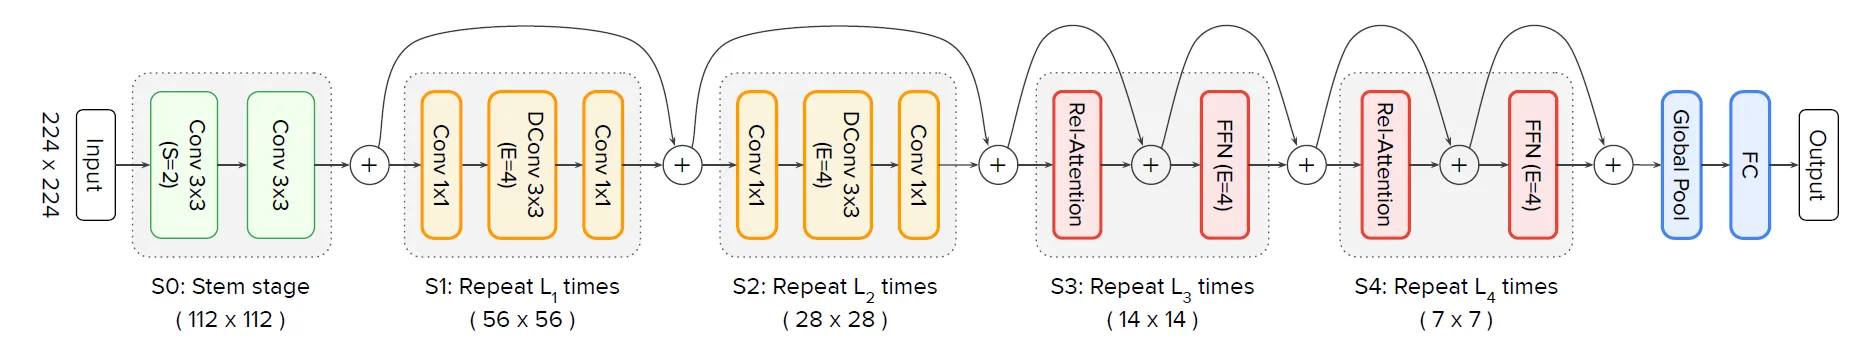
\includegraphics[width=\textwidth]{img_related_work/CoAtNet.png}
    \caption{The CoAtNet architecture.}
    \footnotesize{Sourced from original paper \cite{CoAtNet}.}
    \label{fig:CoAtNet}
\end{figure}

The CoAtNet architecture, which schema is demonstrated in Figure \ref{fig:CoAtNet}, integrates convolutional layers and attention layers in a structured manner to harness the strengths of both. The convolutional layers capture translation equivariance, effectively modeling local patterns, while the attention layers introduce adaptive global feature representation, enhancing the model's capacity to generalize. This combination is achieved by summing a global static convolution kernel with the adaptive attention matrix, either before or after the Softmax normalization. The resulting attention weight is influenced both by the convolutional kernel and the input-adaptive components, ensuring minimal additional computational overhead. The architecture leverages pre-normalization relative attention for improved efficiency.

To train the CoAtNet model, the researchers used the Adam optimizer with a cross entropy loss function as in the original CoAtNet paper (\textit{\cite{CoAtNet}}). They have experimented with different learning rates, number of epochs and data splitting strategies, comparing stratified and random splits to achieve performance optimization.

The experiments were conducted in two different recording environments. First, keystrokes were captured using an iPhone placed on the left side of the laptop on a folded piece of microfiber cloth (to limit any vibration). In the second setting, referred to as 'data recorded by Zoom,' keystrokes were recorded using the Zoom video conferencing app's built-in audio recording function. In this scenario, the victim participated in a Zoom meeting using the MacBook's built-in microphone array, with noise suppression set to the lowest possible level.

After extensive tuning of the hyperparameters, the authors achieved significant results over 1100 epochs. The model achieved an accuracy of 95\% on phone-recorded laptop keystrokes, one of the highest accuracies reported in the literature for classifiers that do not use language models. On data recorded with Zoom, the proposed method yielded an accuracy of 93\%, demonstrating high risk even in situations where the quality of the sound is weakened.

\section{Limitations}

The research discussed in this chapter highlights significant development in the use of deep learning methods for acoustic side-channel attacks. However, each approach also faces significant limitations, which together highlight the complexity of the domain and point to directions for further research.

One recurring challenge is the dependence of accuracy on writing style. Many existing solutions are tailored to individual writing behavior, undermining their ability to generalize to different users. This dependency limits the scalability and practicality of these methods in real-world scenarios, where writing styles can vary widely depending on factors such as user experience, typing speed and individual preferences. Moreover, many methods are dependent on specific keyboard models. Techniques optimized for a particular keyboard often do not work well on others, reducing their versatility. The heavy reliance on the acoustic properties of the keyboard limits the applicability of these models to a wider range of devices, especially since modern keyboards vary widely in design and sound characteristics.

These limitations are further intensified by the shortage of large, diverse datasets. High-performance deep learning models typically require extensive training data to achieve accuracy and reliability. However, collecting such datasets for ASCA is resource-intensive, and additionally they are not publicly available. This may be due to the fear of being used by someone with improper intentions. This limitation significantly hinders the development of zero-shot or few-shot learning capabilities that would otherwise allow models to adapt to new users or environments with minimal data. Without diverse datasets covering different keyboards, typing styles and environmental conditions, generalizing existing approaches remains a major challenge.

Sensitivity to environmental noise is another critical limitation. While some studies have addressed this issue, most do not provide an in-depth analysis of how different types of noise affect model performance. Only a limited number of papers, such as the one written by \textit{\cite{anand2018keyboard}}, have examined the differential effects of noise, revealing how it interferes with classification accuracy. However, a systematic analysis of noise types, sources and mitigation strategies is missing, leaving a gap in understanding the robustness of these models under realistic conditions.

In addition, detection of special characters and keys that require modifiers (such as Shift) is a largely unexplored area. Current approaches mainly focus on alphanumeric keys, and some include detection of punctuation marks. However, no study has comprehensively addressed the challenges of identifying special characters, especially those that require a combination of keystrokes. This omission is compounded by the lack of focus on the peak moment of a keystroke, which could provide critical information for distinguishing such characters.

In conclusion, while the reviewed works make valuable contributions to ASCA, they fall short in addressing key challenges such as typing style dependence, keyboard model specificity, sensitivity to ambient noise and special character detection. The research presented in this paper aims to develop a more generalized, robust and versatile solution that can overcome some of these limitations, paving the way for wider application of acoustic side-channel analysis in real-world settings.



\chapter{Datasets}
The reliability and generalizability of any machine learning model is heavily influenced by the variety and quality of the data used during the training process. In the case of acoustic side-channel attacks, publicly available datasets are very limited, as publishing such recordings poses ethical and security risks. As a consequence, most available datasets have been released under controlled conditions, such as academic research or security contests, and often contain recordings made under specific setups and with limited size. A noticeable trend among these datasets is that many are recorded using Mac keyboards, which influenced the objective of this project. By aligning with the most commonly used data sources, this study is able to make more direct comparisons with existing studies.


\section{Publicly Available Datasets}
\label{publicDatasets}

\subsection{Sonotype Challenge Dataset \protect\footnotemark}
\label{kaggleDataset}

\footnotetext{Available on Kaggle: \url{https://www.kaggle.com/datasets/nguyncaoduy/keystroke-noiseless-final/data}}


This dataset was originally prepared as part of the Sonotype challenge held during the Singapore AI CTF 2024, and was developed and released by the Lost Kids team based on raw audio data provided by the contest organizers. The dataset consists of individual recordings of keystrokes that have been pre-processed to reduce background noise and improve clarity.

Each recording is stored in a separate .wav file, named using a key-<keyname>-<idx> pattern that clearly identifies the key pressed and the sample index. The dataset includes 42 different classes, representing characters a-z, digits 0-9 and some special keys such as comma, period, apostrophe, semicolon, Enter and space. Each class contains about 10 to 20 samples, making it relatively small, but well suited for comparing classification performance on clean, isolated keystroke sounds. Because of its high signal-to-noise ratio and normalized structure, this data set serves as a reliable starting point for model training and controlled evaluation.


\subsection{A Practical Deep Learning-Based Acoustic Side Channel Attack on Keyboards – Associated Dataset \protect\footnotemark}
\label{practicalDataset}

\footnotetext{Available on GitHub: \url{https://github.com/JBFH-Dev/Keystroke-Datasets}}


As part of the work presented in the article "A Practical Deep Learning-Based Acoustic Side Channel Attack on Keyboards" (\textit{\cite{CoAtNet2023}}), the authors published a dataset containing keyboard sound recordings captured under two different conditions.

The first subset was created using the built-in recording function of the Zoom application. Keystroke sounds were captured during a simulated video call session, emulating a scenario in which an acoustic leak might occur on a conference platform. The second subset was recorded locally using a smartphone placed next to the MacBook Pro, laid on a microfiber cloth in order to minimize resonance and undesired noise.

Both subsets contain \texttt{.wav} files, each representing 25 consecutive keystrokes of a single character. The recordings include letters of the alphabet (a-z) and numbers (0-9), with keystrokes performed at natural intervals and pressure levels. Combined, the two subsets yield a total of 1788 labeled audio samples. All samples were collected by the same person in a controlled environment, ensuring consistency of acoustic conditions.

The authors of the dataset verified that the sound quality of the Zoom recordings was comparable to that of locally captured audio. Based on this observation, the two subsets were treated as acoustically equivalent in this study and were concatenated to increase the total number of training samples.


\subsection{Multi-Keyboard Acoustic (MKA) Dataset \protect\footnotemark}
\label{mkaDataset}

\footnotetext{Available on Mendeley Data: \url{https://data.mendeley.com/datasets/bpt2hvf8n3/4}}

The Multi-Keyboard Acoustic (MKA) dataset (\textit{\cite{mka_dataset}}), developed by a research team at the Department of Computer Science at Halabja University, was created to support research on side-channel-based acoustic attacks and keystroke sound classification. It includes a wide range of audio recordings collected in 6 different configurations, using keyboards of different brands and different sound transmissions: HP, Lenovo, MSI, Mac, Messenger and Zoom. The dataset is structured to reflect differences in typing acoustics on different devices, environments and communication platforms.

Each platform-specific subset contains three components: raw recordings, segmented keystroke audio and corresponding feature matrices. The raw data consists of approximately 20-second recordings for each keyboard key, each recording about 30 repeated keystrokes, while the segmented files are short, labeled audio snippets of individual keystrokes. The authors also provided an aggregated version of the dataset, combining all platform data for cross-platform analysis. In addition to the audio, the dataset includes pre-calculated MFCC-based feature matrices and metadata files containing detailed information on the recording configuration, device used and keystroke labels.

Only MacBook keyboard recordings were used for this study, ensuring consistency with other datasets where most of the publicly available keyboard recordings are based on Apple's hardware. Only the raw data section of these recordings was used, and the audio files were manually segmented into individual keystrokes in a manner consistent with the other datasets used in this study. Details of the segmentation process are described in the next section.


\section{Custom Dataset}
\label{customDataset}

In addition to publicly available resources, this study utilised a custom dataset that was specifically designed, recorded, and meticulously processed to enhance the diversity of acoustic environments represented. The creation of this dataset involved extensive planning and  scrupulous preparation of recording settings to capture a broad spectrum of realistic background noises. Recording sessions were conducted in controlled yet varied conditions, deliberately chosen to simulate everyday acoustic scenarios. Furthermore, keys were pressed with intentionally varied strength and speed to capture diverse typing styles, thereby improving the dataset’s generalisability. To ensure high audio quality and consistency, the raw recordings underwent thorough post-processing steps including precise trimming, noise filtering, normalization, and segmentation. The dataset is structured into four distinct subsets, each representing different environmental conditions with varying degrees of acoustic disturbance, enabling more reliable and robust model performance.

\begin{itemize}
    \item \textbf{Clean:} Recorded in a quiet home environment. This subset represents the cleanest data, with minimal background noise and consistent recording conditions. It serves as a baseline for evaluating model performance under ideal conditions.

    \item \textbf{Outdoor Noise:} Captured with the window open, allowing uncontrolled environmental sounds such as passing vehicles, distant conversations, and other street noise to interfere with the recordings.

    \item \textbf{Washing Machine Noise:} Recorded while a washing machine was operating nearby. This introduces low-frequency mechanical noise typical of domestic appliances.

    \item \textbf{Dishwasher Noise:} Collected in the presence of a running dishwasher, adding both rhythmic mechanical sounds and intermittent water-related noises to the background.
\end{itemize}

In each of the four environments, a full set of keys available on the MacBook Pro (14" with M3 processor) keyboard was recorded using the built-in Mac microphone. The keys were pressed sequentially, with careful variations in pressure, click speed, and hand position to reflect natural differences in individual typing behaviour. Each key was initially pressed 15 times per environment; however, in the final segmented version of the dataset, this number may vary between 10 and 15 samples per key due to inconsistencies in signal clarity and the challenges associated with accurately isolating each keystroke. All recordings were captured using the same device and configuration, ensuring internal consistency across subsets. The segmentation process resulted in 3547 labeled audio samples in total. The resulting dataset complements existing online resources by introducing realistic and diverse acoustic conditions, many of which are typically underrepresented in publicly available data. This custom dataset therefore offers a more comprehensive foundation for evaluating model performance in real-world typing scenarios.



\chapter{Methodology}

\section{Research Approach}

This thesis adopts a structured research approach to assess the feasibility and limitations of inferring keystrokes from acoustic side-channel information. The main goal is to evaluate how accurately neural networks, can classify keystrokes based on audio recordings. The experiments are conducted under multiple configurations to reflect different use cases and levels of realism.

\vspace{0.3cm}

The research is first divided into two distinct data setup variants, each corresponding to a different interpretation of the task and potential threat scenario:

\begin{itemize}
    \item \textbf{Alphanumeric-only classification:} This setup restricts classification targets to letters and digits, aligning with most existing work on keystroke recognition. It models scenarios where the attacker aims to recover general text input, such as messages or documents. In this context, small character-level errors may be acceptable if the overall semantic meaning of the message is preserved. This setup emphasizes language-level reconstruction and the model’s ability to recognize linguistic structure, even when the input is partially corrupted.

    \item \textbf{Full-keyboard classification:} This setup includes all available keys on a Mac keyboard, such as punctuation marks, modifier keys (e.g., Shift, Command), and special symbols. It is designed to simulate more sensitive contexts, such as password input or terminal commands, where exact reproduction of the typed sequence is essential. Even a single misclassified character can lead to failed authentication or unintended actions, making this a much stricter and more security-critical task.
\end{itemize}

\vspace{0.3cm}

Each data configuration is then evaluated through two following complementary experimental processes that differ in environmental conditions and research objectives.


\subsection{Controlled Setting}

    % Aims to achieve high classification performance on public, clean datasets to push the boundaries of what is technically possible under ideal conditions. It focuses on evaluating the maximum achievable performance of models built from neural networks when applied to clean, well-labelled audio data. This allows for comparative testing and architecture comparison under ideal conditions.
The first research scheme concerns the potential of various neural network architectures in clean, controlled conditions. The aim is to determine the baseline level of prediction accuracy that can be achieved when the model is trained and tested on selected data sets with minimal interference. These datasets contain high-quality recordings of keyboard typing events, typically segmented and labelled at the keystroke level. The advantage of working in such conditions is that it isolates the model's capabilities from environmental factors, allowing it to focus solely on the neural network's ability to learn and generalise based on the acoustic characteristics of keystrokes.

As part of this experimental direction, many deep learning architectures have been tested, all of which integrate attention mechanisms (\cite{vaswani2017attention}) to varying degrees. Models based on attention mechanisms are particularly well suited to this task due to the nature of the input data – spectrograms of keystroke sounds – where only small, localised areas contain the information necessary for classification. Unlike recurrent architectures or plain CNNs, attention mechanisms allow the model to dynamically focus on these relevant segments without requiring a strict sequential structure or fixed receptive fields.

% The models considered in this track include:
% \begin{itemize}
%     \item Swin Transformer (\cite{swin}), which introduces hierarchical self-attention through local windowing, making it efficient for capturing localized acoustic features.
%     \item CoAtNet (\cite{CoAtNet}), a hybrid architecture that combines convolutional layers with attention modules, benefiting from both local inductive biases and global context modeling.
%     \item MOAT (\cite{MOAT}), which builds on the efficiency of convolutional layers while introducing learnable, spatially dynamic attention mechanisms.
% \end{itemize}

% For this purpose, three neural network-based architectures were explored, each trained and evaluated on parts of three publicly available datasets containing keystroke recordings, mentioned in Section \ref{publicDatasets}, enabling a comparison of different input distributions. This part of the study aims to establish a state-of-the-art benchmark for keypress sound classification and highlight the comparative advantages of different model families under ideal conditions.

For this purpose, three neural network-based architectures were explored. Each model was trained and evaluated using separate subsets of three publicly available keystroke recording datasets, described in Section \ref{publicDatasets}. By splitting the datasets into disjoint training and evaluation sets, we enable a robust comparison of model performance across varying input distributions. This part of the study aims to establish a state-of-the-art benchmark for keypress sound classification and highlight the comparative advantages of different model families under ideal conditions.

\subsection{Real-World Simulation}

Achieving high accuracy in clean conditions shows that acoustic attacks are possible, but does not reflect the complexity of real-world scenarios, where background noise, varying distances, and device diversity pose significant challenges. Therefore, the second part of the experiment aims to assess how well trained models perform in these more realistic and unfavourable conditions. It also serves to explore potential defense mechanisms - for instance, understanding how and when models fail may inform hardware design, microphone shielding, or acoustic noise injection techniques that serve as countermeasures.

In this part of the study, the entire dataset described in Section \ref{customDataset} was used, including both clean and noisy subsets. The \texttt{Clean} subset, recorded in a quiet home environment, serves as a baseline for evaluating model performance under ideal conditions. The remaining subsets include controlled background noise to simulate typical acoustic environments, such as:
\begin{itemize}
  \item sounds from the street, including conversation noise and passing vehicles
  \item sounds from operating household appliances such as washing machines and dishwashers
\end{itemize}


In order to assess generalisation across different domains of noise, two complementary assessment strategies were adopted:

\begin{itemize}
    \item \textbf{Clean-to-noise assessment:} The models were trained from scratch on \texttt{Clean} subset of data, specially recorded audio without background noise, and then evaluated on relevant recordings made in noisy environments. This setup tests whether models trained under ideal conditions retain their predictive ability in the face of acoustic disturbances.

    \item \textbf{Noise-to-clean evaluation:} Conversely, models were trained on noisy recordings and then evaluated on the cleanest recordings available. This approach investigates whether exposure to variability and background noise during training can lead to more robust representations that generalise well even in quiet conditions.
\end{itemize}

By comparing performance across these two settings, the study analyses the asymmetry of generalisation between clean and noisy environments and examines how training conditions affect model robustness.

\vspace{0.7cm}

The results aim to provide a comprehensive understanding of the capabilities and limitations of acoustic side-channel attacks in both ideal and realistic scenarios. They will also be combined with postprocessing performed using Large Language Models (LLMs), offering a hybrid perspective. Even when the raw acoustic model fails to produce perfect predictions, the contextual and syntactic knowledge of language models can be leveraged to correct plausible errors, simulating how an attacker might augment model output with semantic reasoning.

% \vspace{0.5cm}

% Together, these two axes of variation—data scope and environmental condition—allow for a comprehensive analysis of acoustic side-channel vulnerability. They help differentiate between semantic recovery scenarios and exact transcription requirements, and between theoretical feasibility and practical risk.

\section{Data Preparation}

Accurate segmentation and preprocessing of audio signals are key steps in creating reliable classification models. This section describes in detail the process of isolating individual keystroke events from continuous recordings, preparing them for input into machine learning architectures, and ensuring consistency across different datasets.

\subsection{Keystroke Segmentation}

The raw recordings, originating from the datasets described in Sections~\ref{practicalDataset},~\ref{mkaDataset}, and~\ref{customDataset}, each contain a predefined number of consecutive keystrokes per file. To extract individual events, an energy-based segmentation algorithm is applied. The signal is transformed using short-time Fourier transform (STFT), and an energy profile is computed by summing magnitudes across all frequency bins per frame. This profile is min-max normalized to the range [0, 1].

Potential key presses are identified as peaks exceeding a dynamic threshold, with nearby peaks clustered to remove duplicates caused by residual echoes or overlapping energy spikes. An adaptive strategy adjusts the threshold iteratively to match the expected number of key presses and prepares the segmentation to account for any human errors where the actual number of keystrokes differs from the expected count. Around each final timestamp, a fixed-size window is extracted, filtered for overlap, and trimmed for silence. The resulting segments are randomly split into train, validation, and test sets in a 70/15/15 ratio.

\begin{algorithm}[H]
\caption{Keystroke Detection and Segmentation Pipeline.}
\begin{algorithmic}[1]
\REQUIRE Audio signal $x(t)$, expected key count $K$, initial threshold $\theta_0$, adjustment step $\delta$, max retries $R$
\ENSURE List of segmented keystroke signals $\mathcal{S}$

\STATE $E \gets \text{EnergyProfile}(x(t))$ \hfill // Compute energy over STFT frames
\STATE $E \gets \text{Normalize}(E)$ \hfill // Scale energy profile to [0, 1]
\STATE $\theta \gets \theta_0$ \hfill // Set starting threshold
\STATE $r \gets 0$ \hfill // Initialize retry counter

\WHILE{$\text{DetectedPeaks}(E, \theta) \neq K$ \AND $r < R$}
    \STATE $\mathcal{P} \gets \text{DetectPeaks}(E, \theta)$ \hfill // Find local peaks above threshold
    \STATE $\mathcal{P} \gets \text{ClusterPeaks}(\mathcal{P}, \Delta t)$ \hfill // Merge close peaks into single events
    \IF{$|\mathcal{P}| < K$}
        \STATE $\theta \gets \theta - \delta$ \hfill // Too few peaks → lower threshold
    \ELSIF{$|\mathcal{P}| > K$}
        \STATE $\theta \gets \theta + \delta$ \hfill // Too many peaks → raise threshold
    \ENDIF
    \STATE $r \gets r + 1$ \hfill // Increment retry counter
\ENDWHILE

\STATE $\mathcal{W} \gets \text{ExtractWindows}(\mathcal{P}, x(t))$ \hfill // Extract fixed-size segments around each timestamp
\STATE $\mathcal{W} \gets \text{FilterOverlap}(\mathcal{W}, \alpha)$ \hfill // Remove overlapping segments based on threshold $\alpha$
\STATE $\mathcal{S} \gets \text{TrimSilence}(\mathcal{W})$ \hfill // Heuristically trim silence from beginning and end
\STATE $\mathcal{S} \gets \text{SplitSets}(\mathcal{S}, 70/15/15)$ \hfill // Randomly split into train/val/test sets
\RETURN $\mathcal{S}$
\end{algorithmic}
\end{algorithm}


% The raw recordings contain sequences of a specific number of consecutive keystrokes in each file. To extract individual keystrokes, an energy-based segmentation algorithm was used. First, the signal is transformed using a short-time Fourier transform (STFT), then he energy of each time frame is calculated as the sum of the magnitudes in all frequency intervals, resulting in a one-dimensional energy profile of the signal. This profile is then normalised in the min-max range to the range [0, 1] for each recording separately.

% A dynamic threshold mechanism is used to detect potential key presses. Peaks in the normalised energy profile that exceed the initial threshold are selected. These peaks are grouped into clusters if they are within a small time window to eliminate multiple detections of the same key press caused by reverberation or overlapping energy spikes.
% Since recordings are known to contain a fixed number of key presses, an adaptive threshold tuning strategy is used. If too few peaks are detected, the threshold is iteratively lowered; if too many peaks are detected, it is raised. This loop continues until the desired number of events is found or the maximum number of retries is reached. For each final timestamp, a fixed-size audio window is extracted, typically covering a short segment before and after the detected key press to ensure full coverage of the audio event. Overlapping segments are filtered based on a configurable overlap factor to avoid duplicates. After that the segments are trimmed from silence using a heuristic approach based on thresholded amplitude detection, ensuring that only the relevant parts of the keystroke sound are retained. Finally, short audio files are randomly grouped into a train, validation and test set, with a 70/15/15 distribution.

% \begin{figure}[h!]
%   \centering
%   \begin{subfigure}[b]{0.49\textwidth}
%     \centering
%     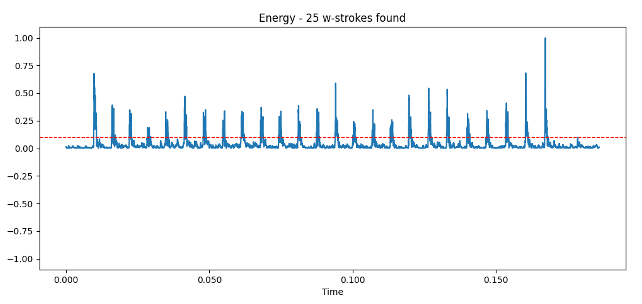
\includegraphics[width=\textwidth]{img_methodology/segmentation_1.png}
%     \label{fig:segmentation_example}
%   \end{subfigure}
%   \hfill
%   \begin{subfigure}[b]{0.49\textwidth}
%     \centering
%     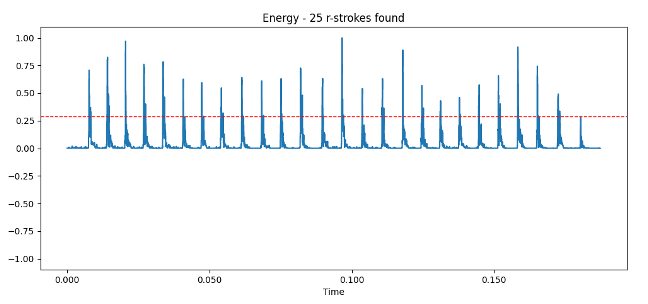
\includegraphics[width=\textwidth]{img_methodology/segmentation_2.png}
%     \label{fig:segmentation_example2}
%   \end{subfigure}
%   \caption{Energy-based segmentation of 'w' and 's' keystroke recordings.}
%   \label{fig:energy_segmentation}
% \end{figure}


\begin{figure}[h!]
  \centering
  \begin{subfigure}[b]{\textwidth}
    \centering
    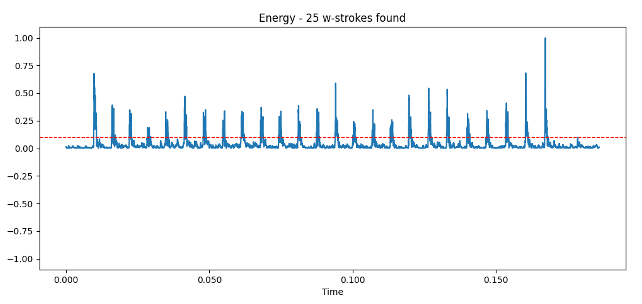
\includegraphics[width=0.8\textwidth]{img_methodology/segmentation_1.png}
    \label{fig:segmentation_example}
  \end{subfigure}
  \hfill
  \begin{subfigure}[b]{\textwidth}
    \centering
    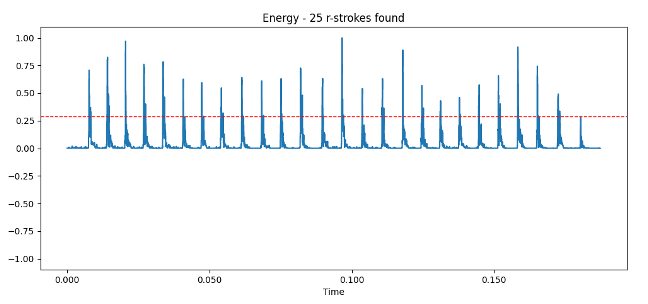
\includegraphics[width=0.8\textwidth]{img_methodology/segmentation_2.png}
    \label{fig:segmentation_example2}
  \end{subfigure}
  \caption{Energy-based segmentation of 'w' and 's' keystroke recordings.}
  \label{fig:energy_segmentation}
\end{figure}

\subsection{Spectrogram Generation and Augmentation}

In downstream modelling, each sound wave is converted into a two-dimensional log-mel spectrogram. This is done using the Short-Time Fourier Transform (STFT), which applies the Fast Fourier Transform (FFT) to short overlapping segments of the audio signal to analyze its frequency content over time. The parameter \( n_{\text{fft}} \) defines the number of samples in each FFT window and thus controls the frequency resolution of the transform. Depending on the length of the audio clip, two STFT configurations are used: for shorter clips (less than 0.5 seconds), $n_{\text{fft}} = 512 $ is used, while for longer clips, $ n_{\text{fft}} = 1024 $ is used. In both cases, the number of mel bands is set to match the target input resolution equal to 64x64, and the stride length is $n_{\text{fft}} / 4$. The amplitude spectrogram is converted to a log-mel representation and then dataset-specific normalization was applied.

\begin{figure}[h!]
  \centering
  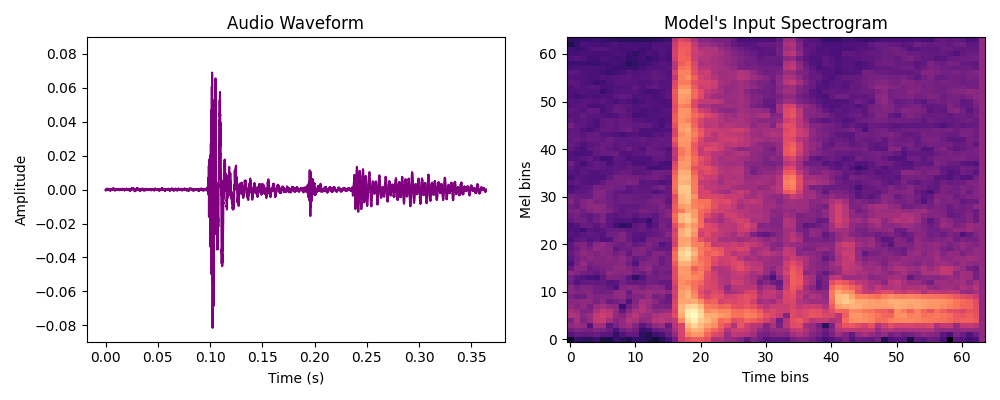
\includegraphics[width=\textwidth]{img_methodology/model_input.png}
  \caption{An example Mel-Spectrogram generated from a keystroke audio clip, used as input to the model.}
  \label{fig:spectrogram_example}
\end{figure}


To standardize input data, spectrograms are padded or cropped to fixed dimensions along time and frequency axes, ensuring uniform input size regardless of clip length or content. This ensures uniformity of input data regardless of differences in clip length or content. Additionally to improve model's generalisation and robustness, several data augmentation techniques are applied online during training with controlled probabilities. These augmentations include:
\begin{itemize}
    \item Time stretching, changing the waveform duration by up to $ \pm 20\% $, applied with 80\% probability,
    \item Frequency masking, in which random frequency bands are zeroed, applied with 40\% probability,
    \item Time masking, which obscures random time intervals, applied with 40\% probability.
\end{itemize}
Each augmentation is applied independently and stochastically, meaning that during each training iteration, spectrograms may or may not be transformed according to these probabilities. This online augmentation strategy enhances the diversity of training samples without increasing dataset size, aiding in preventing overfitting.

\section{Tested Model Architectures}

Deep learning models for image and audio processing have traditionally relied on convolutional neural networks, introduced in \cite{cnn}, not only because of their empirical performance, but also because of well-known inductive biases such as spatial locality and translation invariance. The basis of CNNs is the convolution operation, a linear operation that involves moving a small learning matrix - known as a kernel or filter - over the input tensor. This process calculates local scalar products between the kernel and the input, effectively extracting spatially localised features such as edges, corners and textures. By reusing the same kernel across different spatial dimensions of the input, convolution introduces parameter sharing, which reduces the number of parameters that can be trained and increases statistical efficiency. Furthermore, the receptive field of convolutional layers grows with depth, enabling hierarchical representation learning, in which higher layers capture increasingly abstract concepts.

In contrast, self-attention mechanisms, introduced in \cite{vaswani2017attention}, dispense with such spatial constraints and instead model global interactions from the outset. Self-attention calculates pairwise similarity scores between all input elements - often referred to as tokens or fragments - and uses these scores to generate weighted combinations of input features. This mechanism allows the model to focus on the most relevant parts of the input data, regardless of their spatial distance, making it particularly effective at capturing long-range dependencies. Unlike convolution, which is inherently local and spatially fixed, attention mechanisms are data-driven and dynamic, adapting to the global context of the input data. Although they are more computationally expensive, especially for high-resolution input data, attention-based architectures offer greater modelling flexibility and have a particularly strong impact in areas such as natural language processing and computer vision.

The latest architectures combine the advantages of both paradigms, creating hybrid designs that work well with different types of data and tasks of varying complexity. This paper compares three such architectures: Swin Transformer, CoAtNet, and MOAT.

\subsection{Swin Transformer}

Swin Transformer (\cite{swin}) introduces an innovative hierarchical architecture that adapts the Transformer model to vision-related tasks, eliminating the inefficiency of global self-attention. Unlike the standard Vision Transformer (ViT) (\cite{vit}), which computes attention for all patches globally — leading to high quadratic computational complexity — Swin Transformer restricts self-attention to local, non-overlapping windows. This design significantly reduces the computational load, making it more feasible for high-resolution images.

A key innovation in the Swin Transformer is the use of Shifted Window Self-Attention (SW-MSA). By cyclically shifting the window division between successive layers, the model enables connections between windows without significantly increasing computational complexity. This mechanism facilitates efficient spatial interaction and enhances the model’s ability to capture long-range dependencies, which are typically limited in standard window-based approaches. The schema of the attention mechanism is presented in Figure~\ref{fig:swin}, which shows (a) the hierarchical architecture of Swin Transformer with patch merging between stages, and (b) two successive Swin Transformer blocks alternating between regular (W-MSA) and shifted (SW-MSA) window-based multi-head self-attention.


\begin{figure}
  \centering
  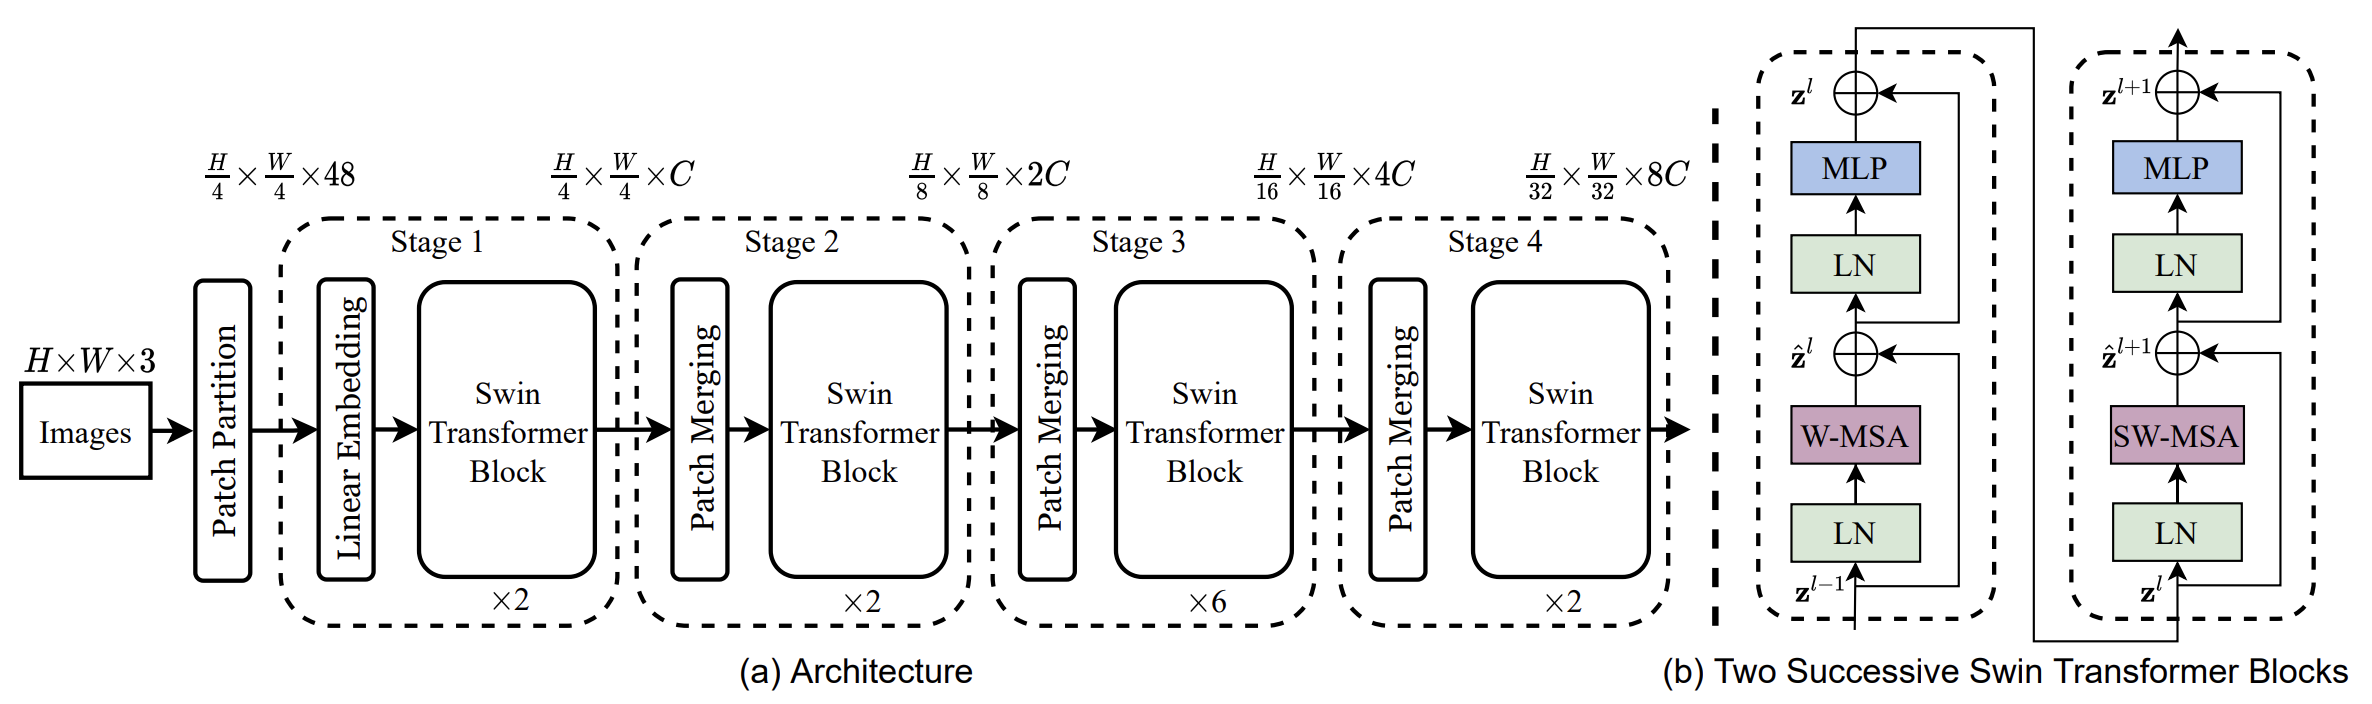
\includegraphics[width=0.9\textwidth]{img_methodology/swin.png}
  \caption{The Swin Transformer architecture.}
  \footnotesize{Sourced from original paper \cite{swin}.}
  \label{fig:swin}
\end{figure}

Swin Transformer has a four-stage structure, each of which gradually reduces spatial resolution by merging fragments while expanding the channel dimension to enable more expressive representations. Each stage consists of a series of Swin Transformer blocks, each containing a multi-head self-attention module operating in windows, followed by a feed-forward network. This hierarchical configuration reflects the design philosophy of convolutional neural networks, providing inductive tendencies such as translation invariance and multiscale.

The Swin Transformer architecture was tested in this work in multiple configurations, combining 2 to 3 modular blocks and offering a scalable solution for different application needs. These configurations cover a wide range of model sizes - from lightweight variants with approximately 1 million trainable parameters to larger models with up to 156 million parameters, which provide greater accuracy in complex calculations.

\subsection{CoAtNet}

CoAtNet (Convolution and Attention Network), presented in \cite{CoAtNet}, is a hybrid vision model designed to combine the structural efficiency of convolutional networks with the dynamic modeling power of Transformer-based self-attention. Rather than treating convolution and attention as separate paradigms, CoAtNet organizes them in a synergistic sequence—allocating convolution to early stages for spatial generalization and attention to later stages for high-level semantic reasoning.

The architecture consists of five progressive stages, with the first three stages implemented using Mobile Inverted Bottleneck Convolution (MBConv) blocks and the final two with Transformer blocks as shown in Figure \ref{fig:CoAtNet}. MBConv blocks are known from efficient architectures like MobileNetV2 (\cite{mobilenetv2}) and EfficientNet (\cite{efficientnet}), and they employ depthwise separable convolutions—a factorized variant of standard convolutions that separates channel-wise spatial filtering from cross-channel mixing. Each MBConv block includes an expansion projection, a depthwise convolution, a squeeze-and-excitation mechanism (\cite{squeeze}) for channel recalibration, and a residual connection to facilitate gradient flow.


The depthwise separable convolution within MBConv allows for substantial computational savings. Specifically, a depthwise convolution applies a single spatial filter per input channel, preserving spatial locality at minimal cost, while the subsequent pointwise (1x1) convolution captures inter-channel dependencies. The inclusion of squeeze-and-excitation operations further refines the activations by adaptively recalibrating channel-wise responses based on global context.

In later stages, CoAtNet transitions to Transformer blocks employing relative self-attention (\cite{relation}). Unlike absolute positional encoding, which binds model behavior to a fixed input size, relative attention introduces location-aware modeling in a resolution-invariant manner. Each attention head in these blocks calculates pairwise similarity between input tokens while incorporating relative position offsets, enabling the model to generalize across different spatial configurations without sacrificing context sensitivity.

CoAtNet improves performance by using convolution in the early layers where general features are learned, and attention in the later layers where capturing complex patterns becomes more important. This design not only improves accuracy but also preserves the hierarchical abstraction inherent to CNNs. With increasing depth, the architecture reduces spatial resolution while expanding the number of channels, allowing higher layers to encode more abstract and semantically rich features.

Experiments covered wide range of architecture variants, from small models having 20M parameters to large ones with 170M parameters, all having the same segment structure, only differing in the number of layers and blocks in each segment.

\subsection{MOAT}

Mobile Convolution with Attention Transformer (MOAT), presented in \cite{MOAT}, refines hybrid vision modeling by focusing on a more granular integration of convolution and attention within a unified micro-architecture. Unlike CoAtNet, which separates convolution and attention into distinct stages, MOAT intertwines them within the same computational block. This tight coupling improves representational power and efficiency, particularly for mobile and edge deployment scenarios.

The design of MOAT stems from two key insights. First, the multi-layer perceptron module typically used in Transformer blocks shares an inverted bottleneck structure with the MBConv block—a widely-used component in mobile networks. However, MBConv includes an additional depthwise 3×3 convolution, multiple normalization layers, and nonlinear activations, allowing it to better model local patterns. Second, in conventional Transformer blocks, downsampling is often achieved via average pooling before the attention mechanism. While computationally efficient, this can weaken the model’s ability to preserve rich representations.

MOAT addresses these challenges by introducing a novel hybrid block that reverses the typical Transformer design. Specifically, MOAT replaces the MLP with an MBConv block and places it before the self-attention layer. This not only equips the architecture with stronger local modeling capabilities through strided depthwise convolution but also delegates the responsibility of downsampling to the convolutional component rather than using pooling. As a result, the network learns more effective downsampling kernels while retaining crucial feature details.

Each MOAT block, presented in Figure \ref{fig:MOAT}, consists of an MBConv unit followed by a multi-head self-attention mechanism, enabling simultaneous extraction of local and global dependencies. This architecture maintains the standard Transformer pipeline of residual connections and normalization but significantly enriches the local context available to each block. Depending on resource availability and input resolution, the attention module can operate globally or within fixed-size windows to optimize the trade-off between accuracy and efficiency.

\begin{figure}[h!]
  \centering
  \includegraphics[width=0.8\textwidth]{img_methodology/MOAT.png}
  \caption{The MOAT block architecture.}
  \footnotesize{Sourced from original paper \cite{MOAT}.}
  \label{fig:MOAT}
\end{figure}

The full MOAT architecture is composed of multiple such hybrid blocks grouped into four stages, progressively reducing spatial resolution while increasing feature depth. The range of models studied in this work spans from compact designs with approximately 20M parameters to large-scale variants with around 116 million parameters, offering deployment flexibility across a range of hardware profiles.


\section{Training and Evaluation}

The training process for the models developed in this study was implemented using the PyTorch library (\cite{pytorch}) and designed with flexibility and robustness in mind, accommodating a range of configurations while maintaining rigorous regularization and optimization strategies. Each model was trained for up to 1000 epochs, allowing for thorough convergence. However, to avoid overfitting and reduce computational overhead, early stopping was employed; training was halted if the validation loss failed to improve for 50 consecutive epochs. This way, only models demonstrating stable and consistent improvement were carried forward.

To optimize the learning process, several well-established optimizers were explored: Adam, AdamW, SGD, and RMSprop (\cite{optimizers}). Each optimizer offers different benefits in terms of stability, convergence speed, and adaptability to sparse or noisy gradients. These were paired with a diverse set of learning rate schedulers to dynamically adjust learning rates throughout training. The schedulers tested included \texttt{StepLR}, \texttt{CosineAnnealingLR}, \texttt{OneCycleLR}, \texttt{CosineAnnealingWarmRestarts}, \texttt{ReduceLROnPlateau}, and chained scheduler combining \texttt{PolynomialLR} with \texttt{CosineAnnealingWarmRestarts}, each bringing unique capabilities in adapting to different loss landscapes and facilitating convergence.

Weight decay was included as a regularization technique to mitigate overfitting by penalizing large weights, encouraging the models to learn simpler, more generalizable representations. Furthermore, dropout was applied within attention mechanisms to add stochasticity during training, helping the models avoid over-reliance on specific pathways and thereby enhancing generalization. In terms of parameter initialization, all convolutional and linear layers were initialized using Kaiming Normal initialization (\cite{kaiming}), which is well-suited for layers followed by ReLU activations. This method helps maintain a healthy variance throughout the network, facilitating stable gradient flow during early training phases.

\vspace{0.3cm}

To evaluate model performance, the \texttt{CrossEntropyLoss} function was used as the primary objective metric during training and validation phases. This loss function is particularly well-suited for multi-class classification problems, as it encourages the model to assign high probability to the correct class while penalizing confident misclassifications.

Beyond the training loss, a broad spectrum of top-$k$ accuracy metrics was reported to assess predictive quality. These included Top-1, Top-2, Top-3, Top-5, and Top-10 accuracy, providing a more comprehensive understanding of how well the model ranked the correct class among its predictions. Such granularity was essential in cases where the exact top prediction was incorrect, but the correct class still appeared among the higher-ranked outputs.

To refine model outputs and assess their semantic alignment with human expectations, an additional post-processing step was introduced using Large Language Models (LLMs). Models such Gemini 2.5 Pro \footnotemark and GPT OSS 120b (\cite{gpt-oss}), were used to clean up raw predictions, resolving inconsistencies and standardizing outputs across various samples, to get the sense of the input.

\footnotetext{Documentation available at: \url{https://cloud.google.com/vertex-ai/generative-ai/docs/models/gemini/2-5-pro}}

Finally, a Levenshtein distance metric (\cite{levenshtein}) was employed to capture the precise number of insertions, deletions, or substitutions required to transform raw output and model's predicted sequence into the corresponding ground truth. This metric provided a fine-grained assessment of output fidelity that goes beyond traditional categorical accuracy, offering insights into how closely the predicted output matches the expected result in practical applications.


\chapter{Results}

This section provides empirical results from the experiments conducted, with the analysis organised according to the evaluation scenarios described in the previous chapter. The results are presented separately for controlled conditions and for scenarios that take into account real-world disturbances, allowing for a clear assessment of the robustness of the models under different input conditions. The comparison covers different architectures and numbers of parameters, examining the impact of model scale changes on predictive power and generalisation. Additionally, for each evaluation scenario, the analysis considers both accuracy and additional performance metrics, enabling a more detailed interpretation of the results.

\section{Architectural Design and Configuration}

The experimental study considers a set of neural network architectures selected to represent diverse design strategies for audio classification. Each architecture is presented with a complete description of its structural composition, including the arrangement and type of layers, dimensionality of intermediate feature maps, and the scaling parameters that define its capacity. The selection spans both high-capacity models aimed at maximizing predictive accuracy and more lightweight designs intended to reduce computational cost. For every configuration, details such as parameter count and approximate floating-point operation requirements (FLOPs) are reported, establishing a clear basis for performance comparisons in the subsequent analysis.

For the Swin Transformer experiments, several configurations were evaluated. Across all setups, the model processed input images using patches of size four, embedded into feature vectors whose dimensions varied according to the configuration. The feed-forward networks within each block had an MLP expansion ratio of 4, and the query, key, and value projections included learnable biases. Absolute positional encoding was not used, allowing the network to rely on relative positional information captured by the shifted window attention mechanism.

The Swin Transformer applies a series of hierarchical, shifted window-based transformer blocks, where the embedding dimension controls the size of the patch representations, the number of blocks per stage determines the depth of hierarchical feature extraction, attention heads enable parallel modeling of patch relationships, and window size sets the local receptive field for self-attention. The combination of these elements allows progressive feature aggregation while maintaining manageable computational cost.

Table \ref{tab:swin_transformer_architectures} summarizes the evaluated Swin Transformer architectures, detailing embedding dimensions, layer depth, attention heads, window sizes, total parameters, and FLOPs.

\begin{table}[h!]
\centering
\caption{Summary of evaluated Swin Transformer architectures.}
\begin{adjustbox}{max width=\textwidth}
\begin{tabular}{lcccccc}
\hline
\textbf{No.} & \textbf{Embed Dim} & \textbf{Blocks/Stage} & \textbf{Attention Heads} & \textbf{Window Size} & \textbf{Params (M)} & \textbf{FLOPs (GFLOPs)} \\
\hline
1 & 96  & [2, 3, 2]      & [3, 8, 12]      & 4 & 5.53   & 0.214 \\
2 & 96  & [2, 2, 6, 2]   & [4, 8, 16, 32]  & 4 & 27.60  & 0.362 \\
3 & 128 & [2, 4, 18, 2]  & [4, 8, 16, 32]  & 8 & 88.52  & 1.374 \\
4 & 192 & [2, 4, 12, 2]  & [4, 8, 16, 25]  & 16 & 156.13 & 2.41 \\
\hline
\end{tabular}
\end{adjustbox}
\label{tab:swin_transformer_architectures}
\end{table}



Following the Swin Transformer experiments, we evaluated several CoAtNet configurations. Each model integrates convolutional and Transformer-based blocks in a multi-stage hierarchy. The hidden dimension at each stage defines feature size, while the number of blocks determines the stage depth. Kernel sizes for convolutional layers, attention head sizes, and expansion ratios for bottleneck and SE modules were kept constant across all stages based on standard defaults. Spatial resolution is progressively reduced between stages, with channel dimensions correspondingly increased to maintain representational capacity.

The evaluated architectures and their stage-wise configurations are summarized in Table \ref{tab:CoAtNet_architectures}, including key hyperparameters.


\begin{table}[h!]
\centering
\caption{Summary of evaluated CoAtNet architectures.}
\begin{adjustbox}{max width=\textwidth}
\begin{tabular}{lccccc}
\hline
\textbf{No.} & \textbf{Blocks per stage} & \textbf{Hidden dimensions} & \textbf{Params (M)} &
\textbf{FLOPs (GFLOPs)} \\
\hline
1 & [2, 2, 2, 2] & [2, 4, 8, 8] & 18.7 & 0.22 \\
2 & [2, 2, 6, 2] & [3, 6, 12, 12] & 24.0 & 0.31 \\
3 & [2, 4, 12, 2] & [4, 8, 16, 16] & 76.4 & 1.7 \\
4 & [2, 4, 12, 2] & [4, 8, 16, 32] & 133.6 & 2.96 \\
\hline
\end{tabular}
\label{tab:CoAtNet_architectures}
\end{adjustbox}
\end{table}

For the MOAT experiments, multiple configurations were evaluated as summarized in Table \ref{tab:MOAT_architectures}. Across all setups, a dropout of 0.3 was applied to both the attention and feed-forward layers, while all other hyperparameters followed the experimental setup and implementation details from the original paper. Each model processed input feature maps through hierarchical transformer blocks, where the embedding dimension defined the size of patch representations, stage depths determined the hierarchical feature extraction, and channel sizes controlled the width of feature maps.

MOAT supports both local and global attention. In this study, each architecture was evaluated with and without window partitions, with window sizes varying between 8 and 16. Windowed attention restricts self-attention to local regions, enabling efficient modeling of local dependencies, while global attention allows full feature interactions, capturing long-range contextual information.


\begin{table}[h!]
\centering
\caption{Summary of evaluated MOAT architectures.}
\begin{adjustbox}{max width=\textwidth}
\begin{tabular}{lccccc}
\hline
\textbf{No.} & \textbf{Depths} & \textbf{Channels} & \textbf{Embed Dim} & \textbf{Params (M)} & \textbf{FLOPs (GFLOPs)} \\
\hline
1 & [2, 2, 4, 2] & [128, 256, 396, 512] & 128 & 14.26 & 0.781 \\
2 & [3, 5, 9, 3] & [128, 384, 512, 1024] & 128 & 71.62 & 2.302 \\
3 & [3, 5, 9, 3] & [256, 512, 768, 1024] & 256 & 116.92 & 5.382 \\
4 & [3, 5, 7, 9, 3] & [128, 256, 512, 768, 1024] & 128 & 121.79 & 2.019 \\
\hline
\end{tabular}
\end{adjustbox}
\label{tab:MOAT_architectures}
\end{table}

The evaluated architectures, Swin Transformer, CoAtNet, and MOAT, cover a wide range of depths, embedding dimensions, channel widths, and attention mechanisms. Testing these models with varying sizes enabled a systematic comparison of performance, efficiency, and the ability to capture local and global dependencies.

\section{Controlled Setting}

The controlled experiments were conducted on clean, publicly available recordings that were manually segmented for training, to evaluate the baseline performance of neural-network based architectures. This setup isolates the classification task from environmental interference and therefore represents the upper bound of achievable accuracy. The analysis focuses on predictive performance across different architectures, parameter scales, and datasets. Particular attention is also given to the trade-off between accuracy and computational cost.

Controlled experiments reveal clear differences in predictive performance between architectures, parameter scales, and datasets. Table \ref{tab:alphanumeric_clean_results} summarizes results achieved by models trained exclusively on alphanumeric key presses a-z0-9. Accross them CoAtNet consistently outperformed other models, with its medium- and large-scale variants (architectures 3 and 4) achieving accuracy equal to 92.21\% in all test recordings. MOAT also showed competitive performance, with several configurations, one exceeding 88\% accuracy. Among them, MOAT with local attention achieved higher accuracy than MOAT with global attention. However, Swin Transformer lagged significantly behind, achieving accuracy in the range of 38–55\%, indicating limited suitability for this classification task in clean conditions.

Importantly, the \textit{Practical dataset} (described in the Section \ref{practicalDataset}) with only alphanumeric keys has also been used in prior research, making it the only directly comparable benchmark. In this setting, training jointly with other datasets led to \texttt{state-of-the-art} performance, with CoAtNet-3 reaching 95.23\% accuracy.


\begin{table}[h!]
\centering
\caption{Test performance of all models on publicly available datasets with alphanumeric keys.}
\begin{adjustbox}{max width=\textwidth}
\begin{tabular}{c|c|c|c|cccc}
\hline
\textbf{Model} & \textbf{Architecture} & \textbf{Window} & \textbf{Loss} & \multicolumn{4}{c}{\textbf{Accuracy [\%]}} \\
\cline{5-8}
       &   \textbf{No.}  &   \textbf{Size}   &   & \textbf{All} & \textbf{Practical} & \textbf{MKA} & \textbf{Noiseless}  \\
\hline
CoAtNet & 3 & - & 0.0028 & \textbf{92.21} & \textbf{95.23} & 83.89 & \textbf{97.06}  \\
CoAtNet & 4 & - & 0.0027 & 90.65 & 91.94 & \textbf{85.00} & 96.08  \\
MOAT & 2 & 16 & 0.0082 & 88.16 & 91.39 & 79.44 & 92.16  \\
MOAT & 4 & 8 & 0.0042 & 86.60 & 88.61 & 80.00 & 91.18  \\
MOAT & 1 & 8 & 0.0060 & 86.29 & 86.67 & 82.78 & 91.18  \\
MOAT & 3 & - & 0.0085 & 85.98 & 88.89 & 78.33 & 89.22  \\
MOAT & 4 & 16 & 0.0050 & 85.67 & 88.89 & 77.22 & 89.22  \\
CoAtNet & 1 & - & 0.0059 & 84.27 & 88.33 & 71.67 & 92.16  \\
CoAtNet & 2 & - & 0.0064 & 83.64 & 86.67 & 75.00 & 88.24  \\
MOAT & 2 & - & 0.0056 & 83.33 & 85.83 & 75.00 & 89.22  \\
MOAT & 4 & - & 0.0049 & 82.71 & 82.22 & 79.44 & 90.20  \\
MOAT & 3 & 16 & 0.0096 & 82.09 & 84.44 & 73.33 & 89.22  \\
MOAT & 1 & - & 0.0065 & 80.06 & 80.83 & 76.11 & 84.31  \\
SwinTransformer & 3 & 8 & 0.0150 & 55.30 & 60.56 & 37.78 & 67.65  \\
SwinTransformer & 2 & 4 & 0.0159 & 53.89 & 58.06 & 39.44 & 64.71  \\
SwinTransformer & 4 & 16 & 0.0203 & 51.15 & 56.50 & 45.00 & 65.53  \\
SwinTransformer & 1 & 4 & 0.0218 & 38.47 & 43.89 & 27.78 & 38.24  \\
\hline
\end{tabular}
\end{adjustbox}
\label{tab:alphanumeric_clean_results}
\end{table}

When comparing architectures within each model family, clear patterns emerge. In the case of CoAtNet, there is a clear correlation between model size and predictive performance: medium- and large-scale architectures (3 and 4) consistently outperform smaller variants, confirming that increasing channel depth and width contributes to higher accuracy. In contrast, MOAT shows relatively uniform performance across all its architectures, with even the smallest configuration achieving accuracy levels comparable to the largest. This suggests that for this task, scaling the MOAT architecture has a limited impact on overall predictive ability. Similarly, Swin Transformer consistently shows poor performance regardless of architecture size, indicating that increasing depth or embedding dimension does not significantly improve its suitability for classifying keystrokes in clean conditions


\begin{table}[h!]
\centering
\caption{Test performance of all models on publicly available datasets with all keys.}
\begin{adjustbox}{max width=\textwidth}
\begin{tabular}{c|c|c|c|cccc}
\hline
\textbf{Model} & \textbf{Architecture} & \textbf{Window} & \textbf{Loss} & \multicolumn{4}{c}{\textbf{Accuracy [\%]}} \\
\cline{5-8}
       &   \textbf{No.}  & \textbf{Size}&        & \textbf{All} & \textbf{Practical} & \textbf{MKA} & \textbf{Noiseless}  \\
\hline
CoAtNet & 3 & - & 0.0024 & \textbf{90.94} & \textbf{93.33} & 85.08 & \textbf{98.31}  \\
CoAtNet & 4 & - & 0.0020 & 90.82 & 93.06 & \textbf{87.12} & 93.22  \\
MOAT & 3 & - & 0.0034 & 89.65 & 92.22 & 84.07 & 95.76  \\
MOAT & 1 & - & 0.0037 & 87.71 & 89.44 & 85.42 & 88.14  \\
MOAT & 3 & 16 & 0.0078 & 86.03 & 88.89 & 79.66 & 93.22  \\
MOAT & 1 & 8 & 0.0043 & 85.77 & 86.94 & 83.73 & 87.29  \\
MOAT & 2 & 16 & 0.0044 & 84.48 & 84.72 & 82.03 & 89.83  \\
CoAtNet & 1 & - & 0.0044 & 83.31 & 84.44 & 79.32 & 89.83  \\
MOAT & 4 & 8 & 0.0036 & 82.15 & 81.39 & 81.02 & 87.29 \\
MOAT & 2 & - & 0.0039 & 81.63 & 80.56 & 80.68 & 87.29 \\
CoAtNet & 2 & - & 0.0069 & 78.78 & 80.56 & 76.27 & 79.66  \\
MOAT & 4 & - & 0.0140 & 61.84 & 59.72 & 67.46 & 54.24  \\
SwinTransformer & 3 & 8 & 0.0101 & 58.47 & 57.50 & 53.56 & 73.73  \\
SwinTransformer & 2 & 4 & 0.0118 & 54.59 & 52.22 & 55.25 & 60.17  \\
SwinTransformer & 4 & 16 & 0.0131 & 47.50 & 68.33 & 49.49 & 54.24  \\
SwinTransformer & 1 & 4 & 0.0168 & 39.07 & 43.33 & 37.29 & 30.51  \\
% (one more MOAT to be added - its running) \\
\hline
\end{tabular}
\end{adjustbox}
\label{tab:all_keys_clean_results}
\end{table}

A similar pattern was observed for models trained using all keys on the Mac keyboard (Table \ref{tab:all_keys_clean_results}). CoAtNet again achieved the best results, with architectures 3 and 4 achieving accuracy above 90\% and standing out in the recordings from Noiseless dataset (98.31\% and 93.22\%, respectively). MOAT ranked just behind, with its medium and large variants maintaining an accuracy of 86-90\% and showing resilience across all subsets. Swin Transformer remained the weakest architecture, achieving an overall accuracy of less than 59\%. Compared to the alphanumeric case, accuracy decreased slightly (approximately 0–2\% for the strongest models), which is expected due to the increased difficulty of the task. The dataset of all keys contains a larger number of classes, which makes classification more difficult, but both CoAtNet and MOAT maintained high performance, highlighting their scalability to more complex label spaces.


\begin{table}[h!]
\centering
\caption{Top-$k$ accuracies of the best models using alphanumeric keys.}
\begin{adjustbox}{max width=\textwidth}
\begin{tabular}{c|c|c|cccccc}
\hline
\textbf{Model} & \textbf{Architecture} & \textbf{Window} & \multicolumn{6}{c}{\textbf{Accuracy (\%)}} \\
\cline{4-9}
 & \textbf{No.} & \textbf{Size} & \textbf{Top-1} & \textbf{Top-2} & \textbf{Top-3} & \textbf{Top-4} & \textbf{Top-5} & \textbf{Top-10} \\
\hline
CoAtNet & 3 & - & \textbf{92.21} & \textbf{96.57} & \textbf{97.82} & \textbf{98.29} & \textbf{98.75} & 99.53 \\
MOAT & 2 & 16 & 88.16 & 95.48 & 97.04 & 97.66 & \textbf{98.75} & \textbf{99.69} \\
SwinTransformer & 3 & 8 & 55.30 & 71.81 & 78.50 & 84.27 & 88.47 & 95.02 \\
\hline
\end{tabular}
\end{adjustbox}
\label{tab:alphanumeric_top_k_accuracies}
\end{table}

To provide a more detailed understanding of model performance, top-$k$ accuracy metrics were calculated for the best-performing models on both key sets. The inclusion of top-$k$ metrics provides an additional layer of insight into model performance beyond the standard top-1 accuracy. As shown in Tables \ref{tab:alphanumeric_top_k_accuracies} and \ref{tab:all_keys_top_k_accuracies}, both CoAtNet and MOAT reach over 97\% top-3 accuracy and exceed 99\% top-10 accuracy on both datasets. This indicates that while the exact keystroke may not always be ranked first, the correct class is almost always present within the first few predictions. From a practical standpoint, this drastically reduces the space of possible keystrokes when attempting to reconstruct typed input, as the candidate set can be narrowed down to only a handful of keys with very high certainty. Consequently, these results highlight that even in the presence of classification uncertainty, the models remain highly effective for keystroke inference tasks.

\begin{table}[h!]
\centering
\caption{Top-$k$ accuracies of the best models all keys.}
\begin{adjustbox}{max width=\textwidth}
\begin{tabular}{c|c|c|cccccc}
\hline
\textbf{Model} & \textbf{Architecture} & \textbf{Window} & \multicolumn{6}{c}{\textbf{Accuracy (\%)}} \\
\cline{4-9}
 & \textbf{No.} & \textbf{Size} & \textbf{Top-1} & \textbf{Top-2} & \textbf{Top-3} & \textbf{Top-4} & \textbf{Top-5} & \textbf{Top-10} \\
\hline
CoAtNet & 3 & - & \textbf{90.94} & \textbf{97.02} & \textbf{98.19} & \textbf{98.58} & \textbf{98.84} & 99.48 \\
MOAT & 3 & - & 89.65 & 96.38 & 98.06 & 98.45 & 98.58 & \textbf{99.61} \\
SwinTransformer & 3 & 8 & 58.47 & 74.26 & 80.47 & 84.48 & 87.32 & 93.79 \\
\hline
\end{tabular}
\end{adjustbox}
\label{tab:all_keys_top_k_accuracies}
\end{table}



\begin{figure}[h!]
\centering

\begin{subfigure}{\linewidth}
    \centering
    \begin{minipage}{0.45\linewidth}
        \centering
        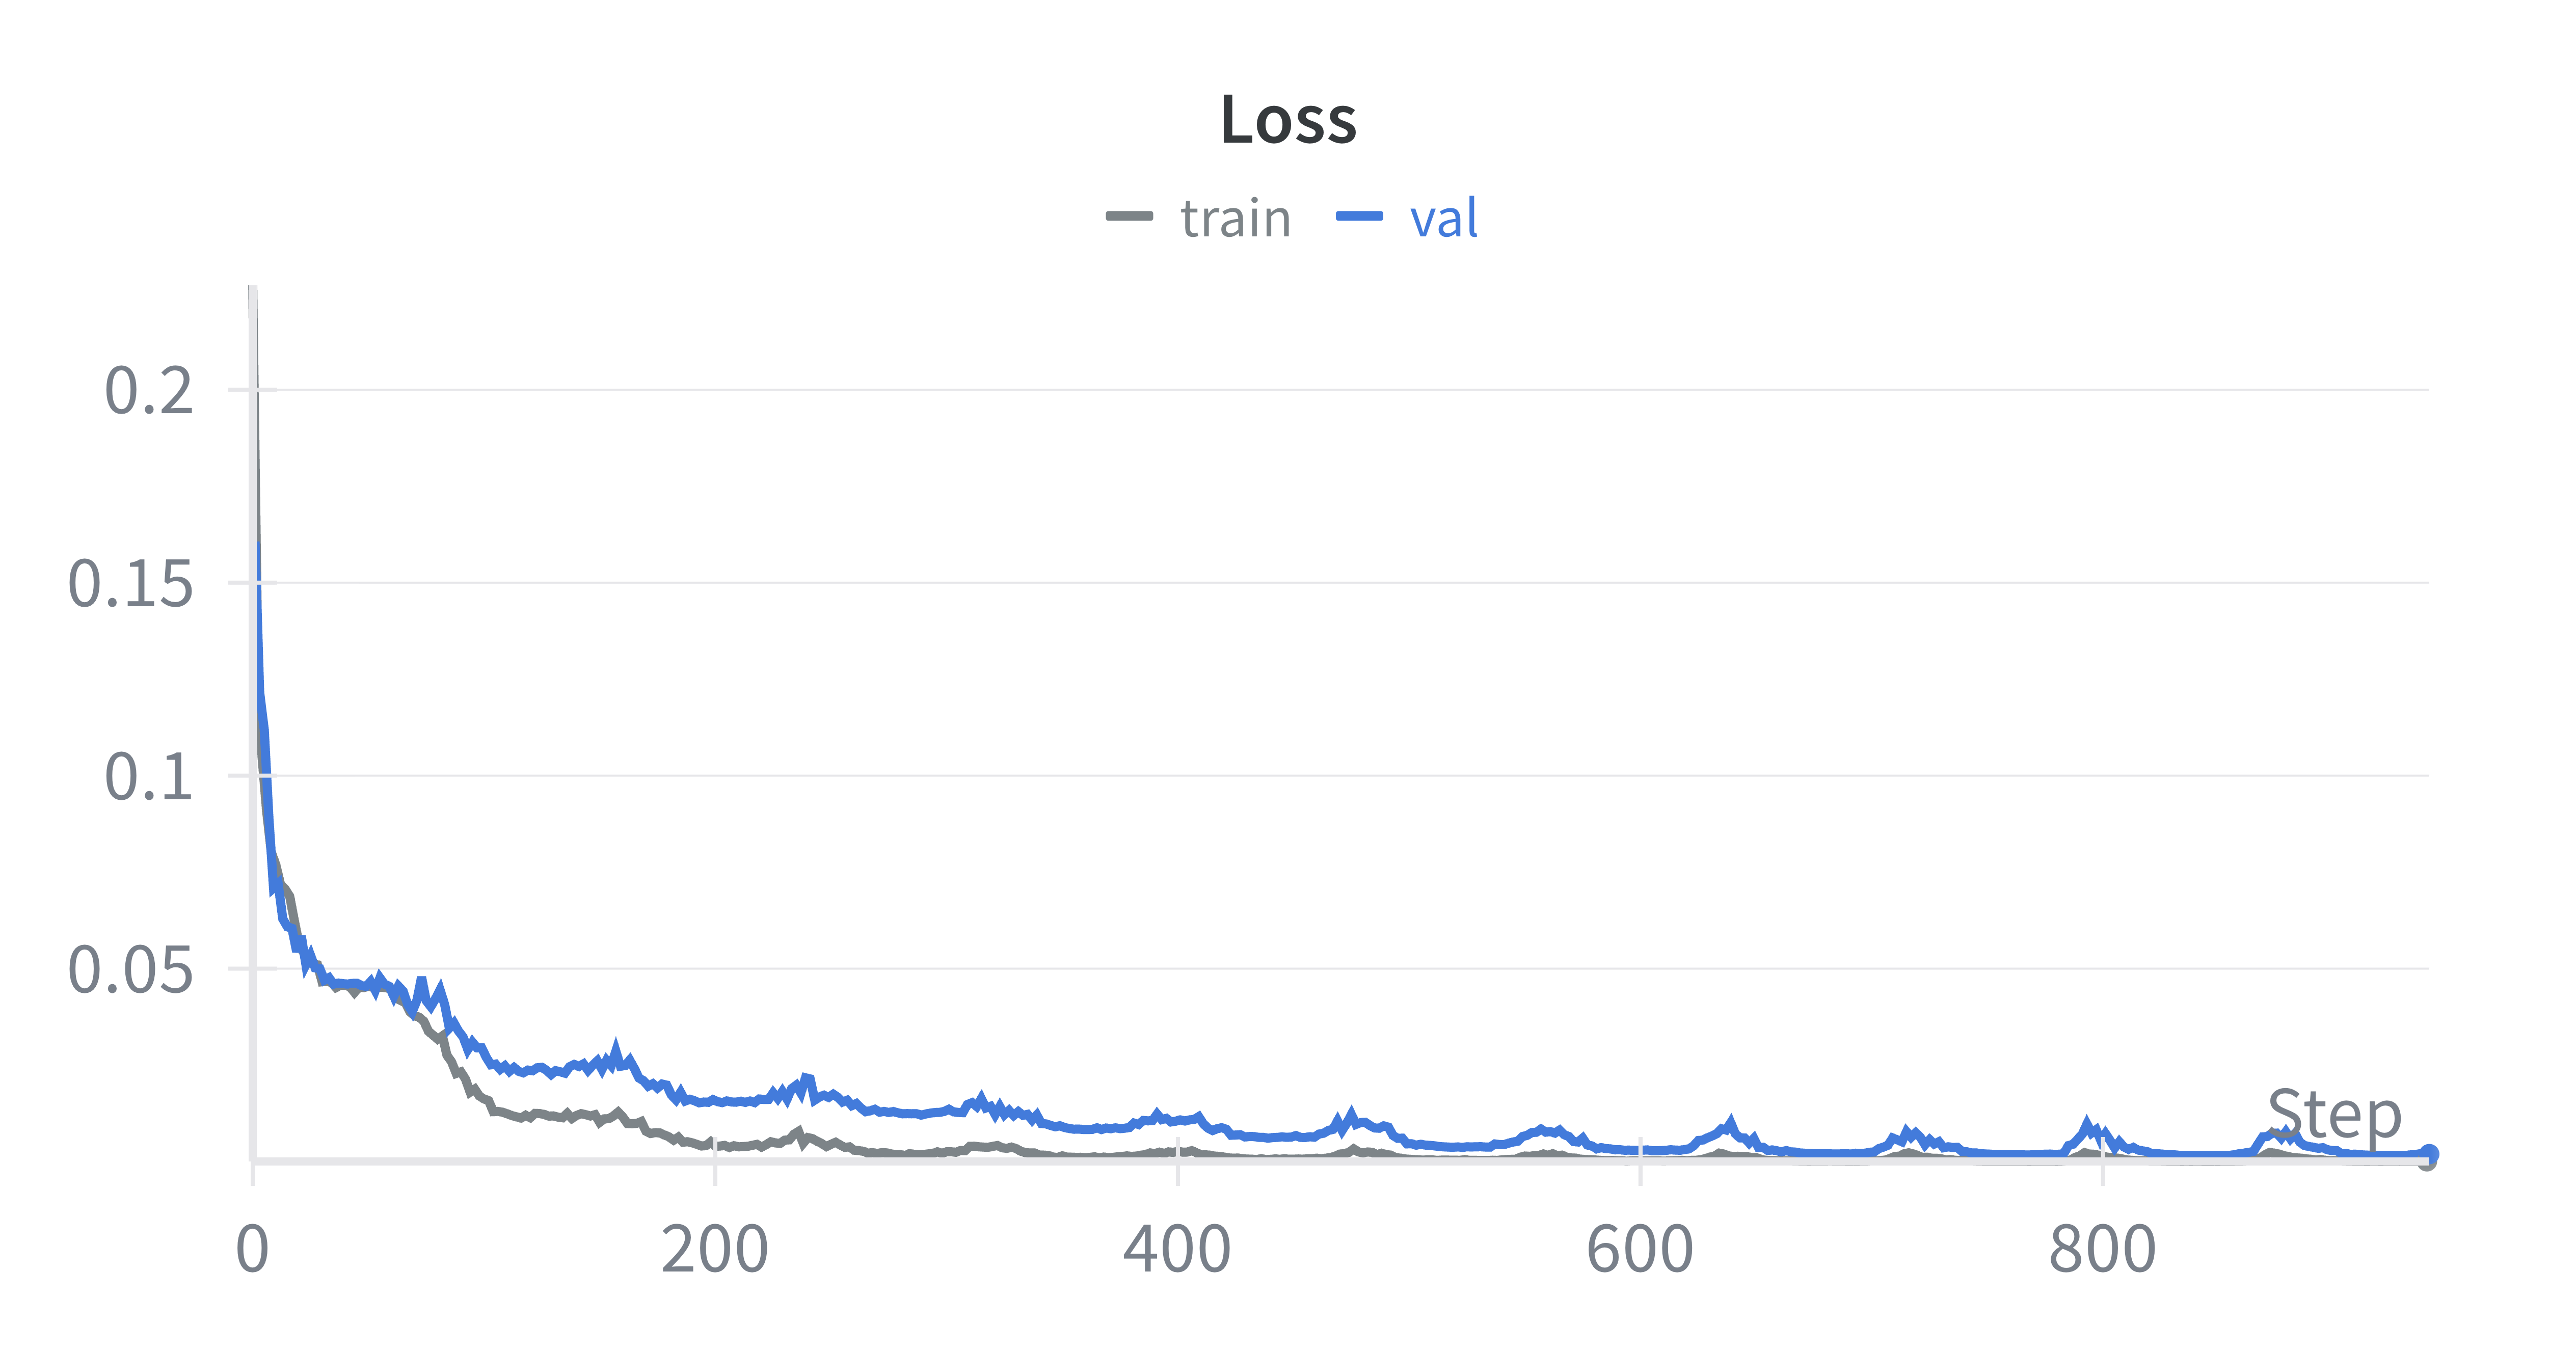
\includegraphics[width=\linewidth]{img_results/loss_alphanum.png}
    \end{minipage}
    \hfill
    \begin{minipage}{0.45\linewidth}
        \centering
        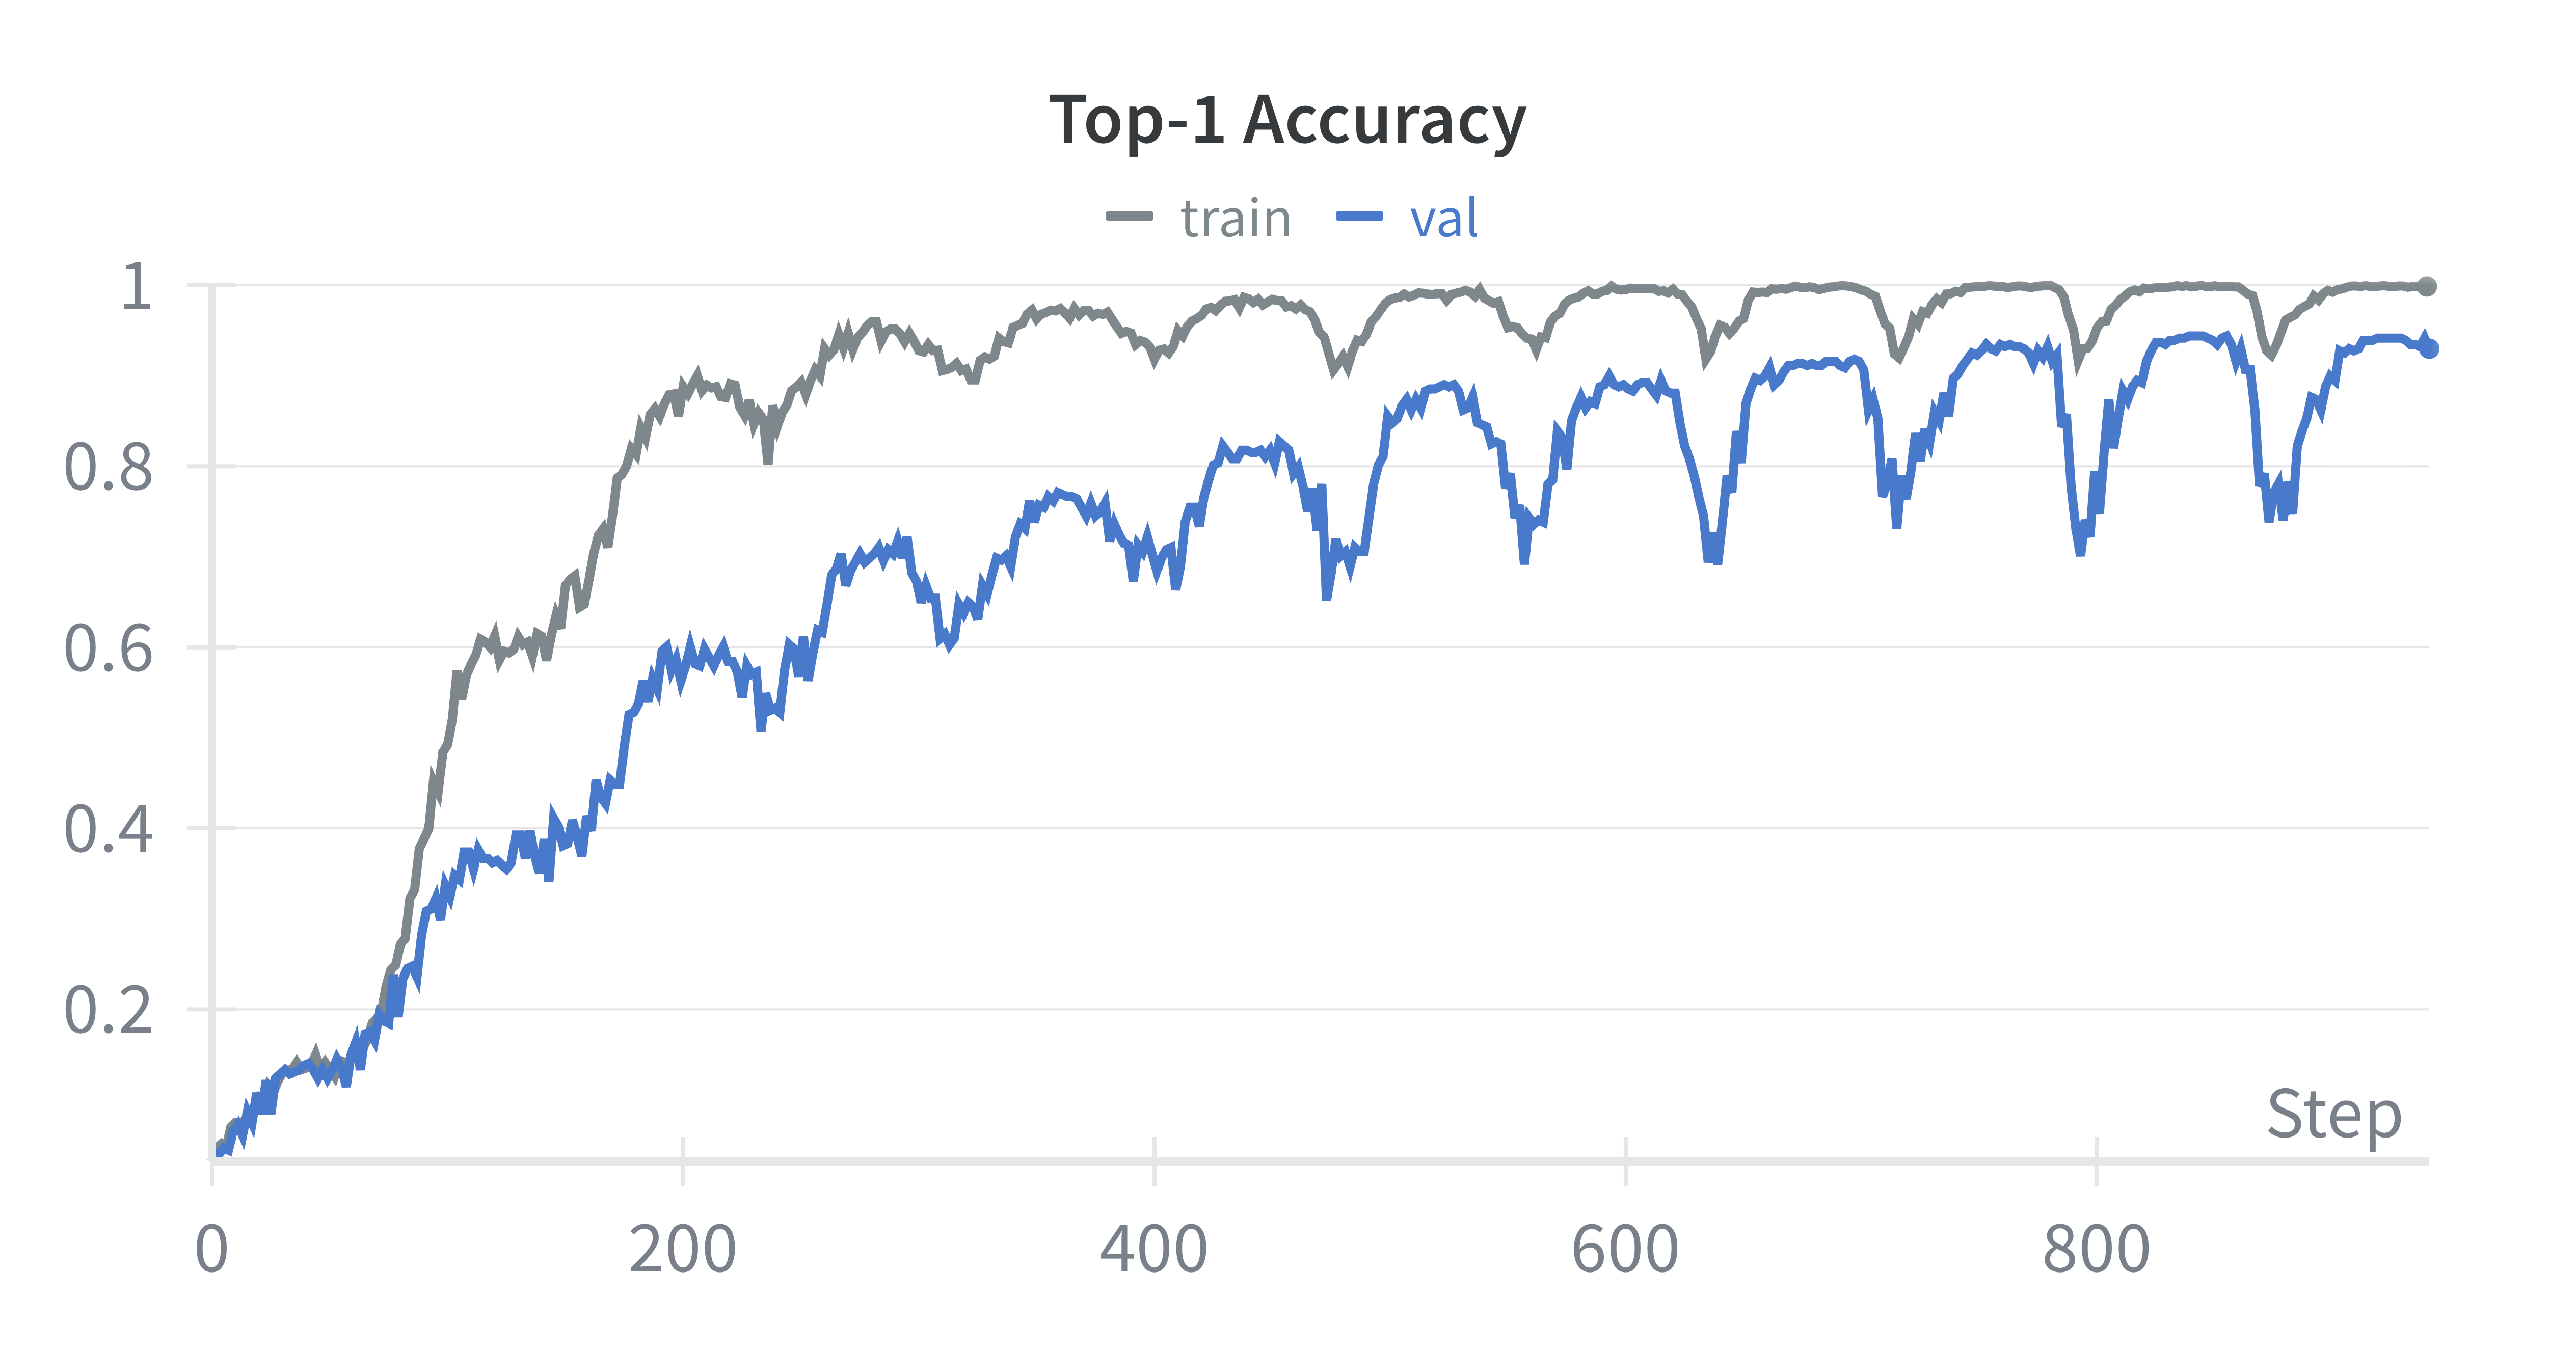
\includegraphics[width=\linewidth]{img_results/acc_alphanum.png}
    \end{minipage}
    \caption{Alphanumeric keys}
\end{subfigure}
\vspace{0.5em}
\begin{subfigure}{\linewidth}
    \centering
    \begin{minipage}{0.45\linewidth}
        \centering
        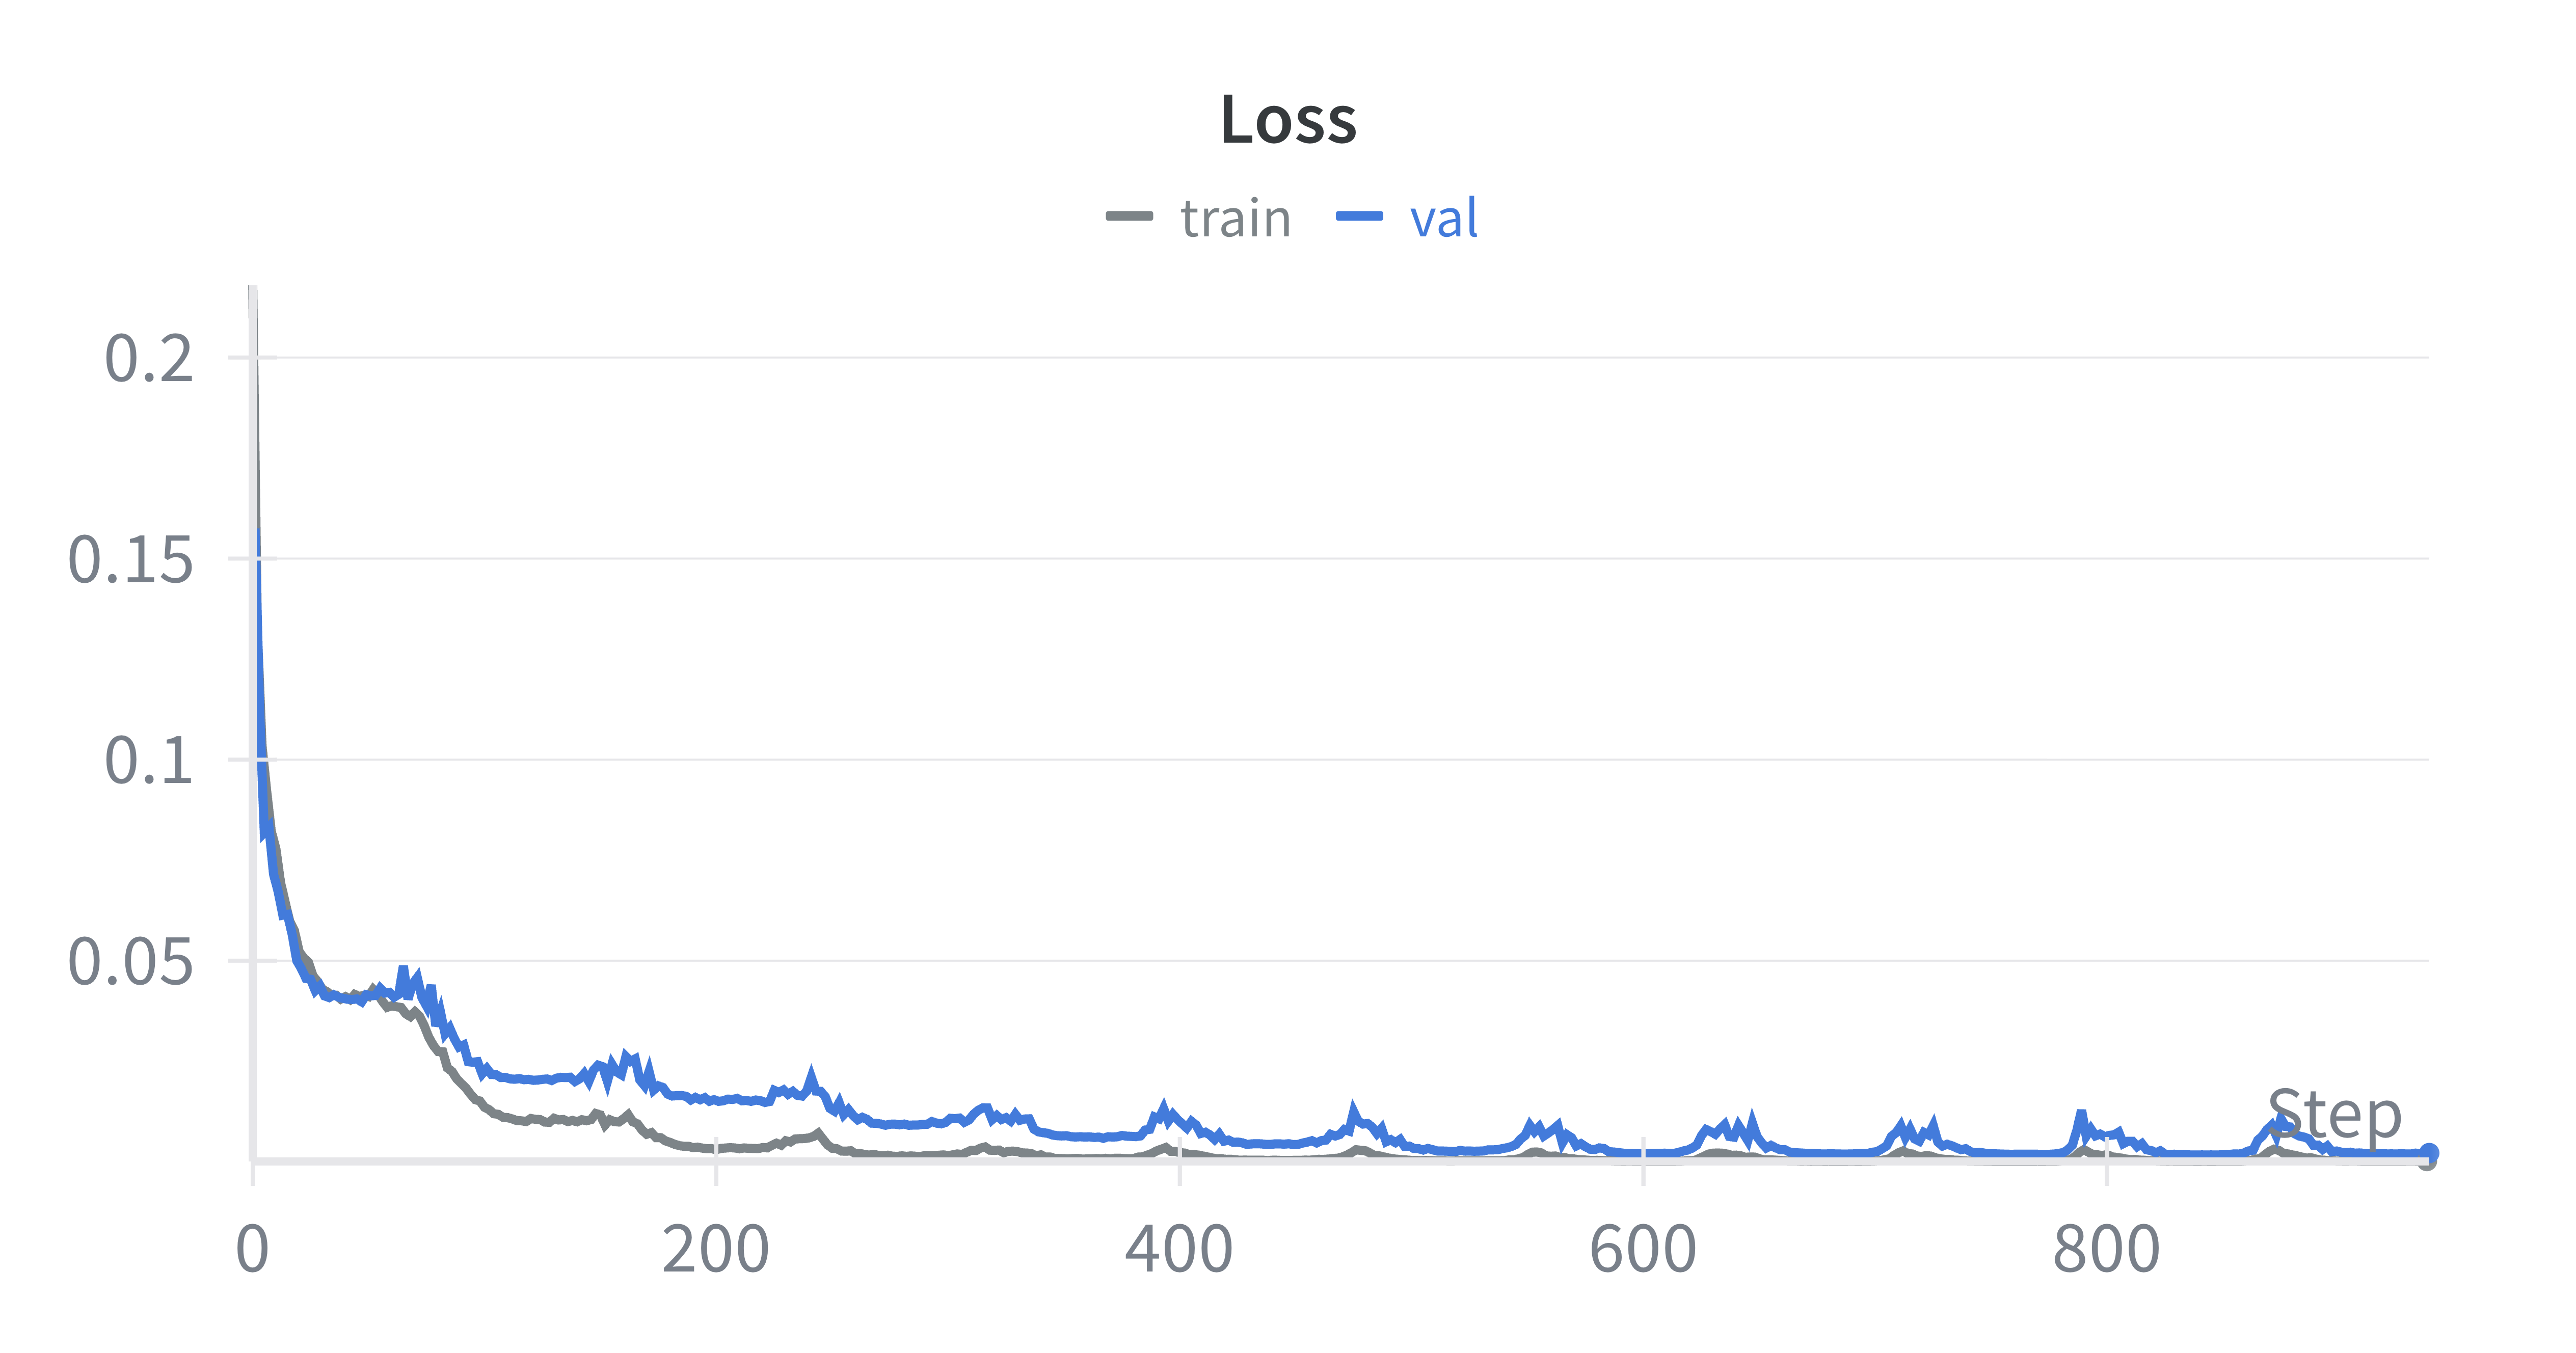
\includegraphics[width=\linewidth]{img_results/loss_all.png}
    \end{minipage}
    \hfill
    \begin{minipage}{0.45\linewidth}
        \centering
        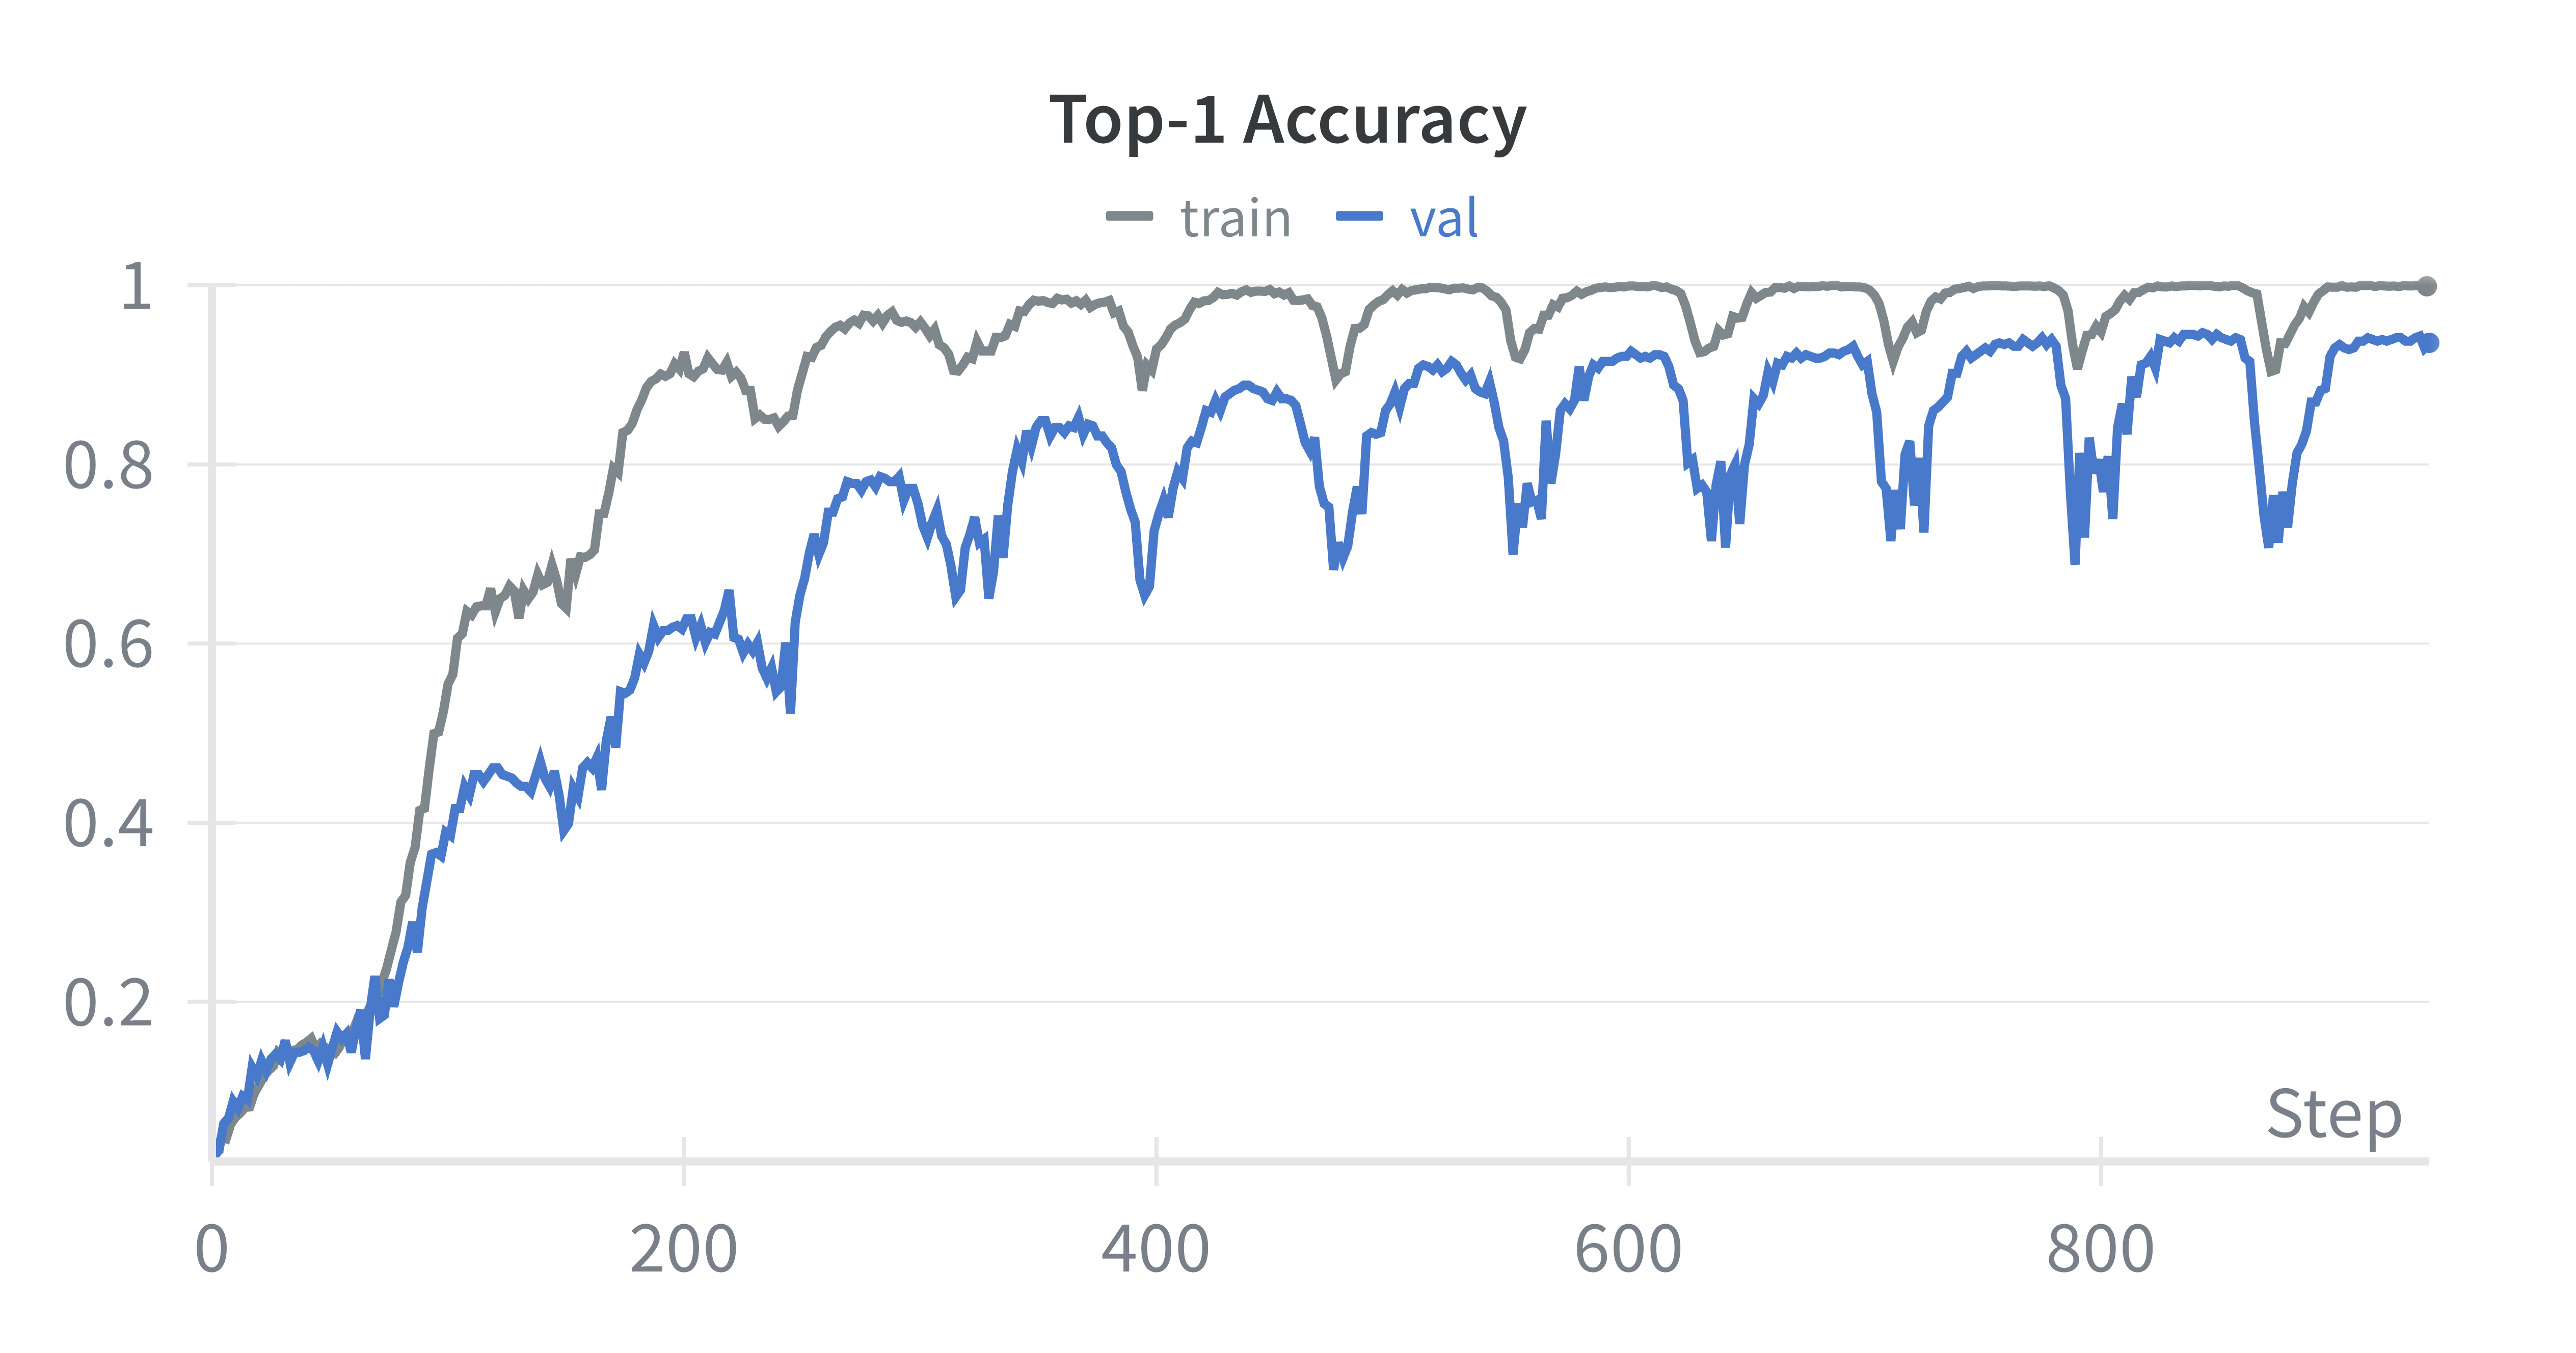
\includegraphics[width=\linewidth]{img_results/acc_all.png}
    \end{minipage}
    \caption{All keys}
\end{subfigure}

\caption{Training histories of the best CoAtNet-3 architectures on different sets of keys.}
\label{fig:training_histories}
\end{figure}

In addition to the top-$k$ results, training histories and confusion matrices were analyzed to provide further insight into convergence and error patterns. The training curves presented in Figure  \ref{fig:training_histories} indicate that, in the initial epochs, the models primarily adapted to the training subset, while validation accuracy gradually approached training performance over time. The use of the Cosine Annealing scheduler for learning rate facilitated sufficient exploration during optimization while maintaining stable convergence.


\begin{figure}[h!]
  \centering
  \includegraphics[width=0.65\linewidth]{img_results/cm_all_CoAtNet_alphanum.png}
  \caption{Confusion matrix of the best CoAtNet-3 model on alphanumeric keys.}
  \label{fig:confusion_matrix_alphanum}
\end{figure}

\begin{figure}[h!]
  \centering
  \includegraphics[width=0.8\linewidth]{img_results/cm_all_CoAtNet_all.png}
  \caption{Confusion matrix of the best CoAtNet-3 model on all keys.}
  \label{fig:confusion_matrix_all}
\end{figure}

Confusion matrices (Figures \ref{fig:confusion_matrix_alphanum} and \ref{fig:confusion_matrix_all}), presented for the best-performing models on both key sets, confirm that an accuracy level of around 90\% corresponds to strong predictive performance. While occasional misclassifications occur, these are largely restricted to acoustically similar keys or those located adjacently on a keyboard layout, which aligns with expected error patterns. In practice, errors most often arise between keys with similar shapes and sizes or those positioned close to one another—for instance, \texttt{(k, j)} or consecutive numbers when trained on alphanumeric keys only, and \texttt{(j, u)}, \texttt{(a, s)}, \texttt{(l, k)}, or modifier pairs such as \texttt{(left control, left option)} in the full-key setup. Detailed confusion matrices for individual public datasets are provided in the Appendix for completeness.

\subsection*{Text Reconstruction}

To further assess the practical usefulness of the models in real text reconstruction, predictions were evaluated using the Levenshtein distance. This metric quantifies the edit distance between predicted and ground-truth sequences, providing a direct measure of how closely the reconstructed text matches the intended input. In addition, LLM-based correction was utilised on raw model outputs, to see if this approach could enhance performance. This step simulates realistic post-processing, where an LLM leverages linguistic context to reduce residual errors and improve readability of reconstructed text.
\newpage
For this evaluation, three sentences were selected to test the models’ ability to reconstruct natural text:
\begin{enumerate}
  \item \textit{Artificial Intelligence has been part of our world for 75 years now.}
  \item \textit{In order to succeed, we must first believe that we can.}
  \item \textit{Life is a journey, not a destination.}
\end{enumerate}
The characters required to form each sentence were randomly sampled from the test dataset, and the corresponding keystroke recordings were fed into the models. This ensured that the evaluation was grounded in actual acoustic samples rather than synthetic input.

When models trained with full set of keys were assessed, the full set of characters required to recreate each sentence was included, preserving case sensitivity. The only simplification applied was that modifier keys (e.g., Shift) were assumed to affect only the immediately following character, since detecting exact release times is difficult in practice. In contrast, evaluation on the alphanumeric-only dataset simplified the problem: sentences were transformed into lists of lowercase words without punctuation, reflecting the reduced output space of these models.

The LLM prompts used for correction were tailored to the two prediction scenarios. For alphanumeric-only outputs, the LLM received a list of lowercase keypresses grouped into words, with instructions to correct obvious substitutions while preserving both order and length of the sequence. For all-key outputs, the input included alphanumeric and special keys (e.g., \texttt{Shift}, \texttt{Caps}, \texttt{Ctrl}), and the LLM was guided to reconstruct coherent sentences while respecting key semantics. Crucially, the prompts framed the inputs explicitly as predicted keypresses, not free text, and instructed the LLM to treat them as noisy model outputs to be repaired. This context ensured that the LLM corrected systematic misclassifications in a way consistent with keystroke-level predictions, rather than performing generic spell-checking.



As an example, for the first sentence, including all keys on the keyboard, the best models predicted:

\begin{center}
\textbf{CoAtNet:} \textit{Artificial Intelligence has been part of our world for 75 years now.} \\
\textbf{MOAT:} \textit{Artificial Intelligence haa been part 0f our world for 75 years n/w.}
\textbf{SwinTransformer:} \textit{Srtificial (lcmd)unrellige0ce has be6n paet of our 0orld gor 75 uears now.}
\end{center}

These examples show that while the overall structure of the sentence was captured by both models, small character-level misclassifications remained in MOAT predictions, which could be easily corrected by a human reader or through LLM-based post-processing. However as expected by the accuracy results, SwinTransformer's output contains more errors, making the final output more difficult to read.

Following this example, a comparative analysis across all architectures is provided, where for each architecture the best-performing model per key set is summarized in Table~\ref{tab:levenshtein_results}. Each Levenshtein distance value reported in the table represents the average over three separate runs, where in each run a different set of recordings from the test dataset was used for the sentences. This design ensures that the results capture variability across recordings and provide a more robust measure of reconstruction performance. Both raw predictions and outputs refined with LLM-based correction (Gemini 2.5 Pro and GPT-OSS 120b) are reported, highlighting baseline model capability as well as the benefit of contextual post-processing.

\begin{table}[h!]
\centering
\caption{Levenshtein distance results for text reconstruction tasks.}
\begin{adjustbox}{max width=\textwidth}
\begin{tabular}{c|c|c|c|c|c}
\hline
\textbf{Model} & \textbf{Keys} & \textbf{Sentence}  &  \multicolumn{3}{c}{\textbf{Levenshtein Distance}} \\
\cline{4-6}
       & & \textbf{No.}& \textbf{Raw}  &   \textbf{Gemini 2.5 Pro}   &  \textbf{GPT-OSS 120b} \\
\hline
\multirow{6}{*}{CoAtNet} & \multirow{3}{*}{Alphanumeric} & 1 & 1 & 0 & 1 \\
& & 2 & 5 & 0 & 0 \\
& & 3 & 0 & 0 & 0 \\
\cline{2-6}
& \multirow{3}{*}{All} & 1 & 1 & 0 & 1\\
& & 2 & 3 & 0 & 5\\
& & 3 & 0 & 0 & 0\\
\hline

\multirow{6}{*}{MOAT} & \multirow{3}{*}{Alphanumeric} & 1 & 3 & 0 & 0 \\
& & 2 & 3 & 0 & 0 \\
& & 3 & 2 & 0 & 0 \\
\cline{2-6}
& \multirow{3}{*}{All} & 1 & 3 & 2 & 1\\
& & 2 & 8 & 0 & 2 \\
& & 3 & 3 & 0 & 0 \\
\hline

\multirow{6}{*}{SwinTransformer} & \multirow{3}{*}{Alphanumeric} & 1 & 14 & 1 & 7 \\
& & 2 & 7 & 0 & 0 \\
& & 3 & 5 & 0 & 0 \\
\cline{2-6}
& \multirow{3}{*}{All} & 1 & 10 & 1 & 6 \\
& & 2 & 7 & 0 & 8 \\
& & 3 & 7 & 0 & 8\\
\hline
\end{tabular}
\end{adjustbox}
\label{tab:levenshtein_results}
\end{table}

\vspace{1em}

From the results, can be seen that while not perfect in every case, the predictions achieve satisfactorily low Levenshtein distances. In general, Gemini provides slightly better post-processing corrections than GPT-OSS, and both LLMs are generally able to correct residual errors, fully reconstructing the original keypress sequences.

\section{Real-World Simulation}


This section presents the evaluation of model performance under more realistic conditions, using the fully customised dataset, described in Section \ref{customDataset}, which was created by the author of this thesis to imitate natural home background noises. Unlike the controlled experiments, these results reflect the challenges posed by environmental noise, varying recording distances, and device variability, providing a better estimate of practical applicability. Tables~\ref{tab:custom_alphanumeric} and \ref{tab:custom_all_keys} summarize the performance of models trained on the full dataset, including both clean and noisy subsets.


\begin{table}[h!]
\centering
\caption{Test performance of  models on the custom dataset with only alphanumeric keys.}
\begin{adjustbox}{max width=\textwidth}
\begin{tabular}{c|c|c|c|ccccc}
\hline
\textbf{Model} & \textbf{Architecture} & \textbf{Window} & \textbf{Loss} & \multicolumn{5}{c}{\textbf{Accuracy [\%]}} \\
\cline{5-9}
       &   \textbf{No.}  &   \textbf{Size}   &   & \textbf{All} & \textbf{Clean} & \textbf{Window} & \textbf{Dishwasher} & \textbf{Washing Machine}  \\
\hline
MOAT & 3 & - & 0.0062 & \textbf{81.09} & \textbf{95.0} & 69.16 & 82.41 & \textbf{78.70} \\
CoAtNet & 4 & - & 0.0054 & 80.38 & \textbf{95.0} & \textbf{71.96} & \textbf{83.33} & 72.22 \\
\hline
\end{tabular}
\end{adjustbox}
\label{tab:custom_alphanumeric}
\end{table}


\begin{table}[h!]
\centering
\caption{Test performance of models on the custom dataset with all keys.}
\begin{adjustbox}{max width=\textwidth}
\begin{tabular}{l|c|c|c|ccccc}
\hline
\textbf{Model} & \textbf{Architecture} & \textbf{Window} & \textbf{Loss} & \multicolumn{5}{c}{\textbf{Accuracy [\%]}} \\
\cline{5-9}
       &   \textbf{No.}  &   \textbf{Size}   &   & \textbf{All} & \textbf{Clean} & \textbf{Window} & \textbf{Dishwasher} & \textbf{Washing Machine}  \\
\hline
MOAT & 4 & 16 & 0.0058 & \textbf{85.68} & \textbf{95.86} & \textbf{76.47} & \textbf{87.77} & \textbf{83.60} \\
CoAtNet & 4 & - & 0.0057 & 84.72 & \textbf{95.27} & 74.87 & \textbf{87.77} & 82.01 \\
\hline
\end{tabular}
\end{adjustbox}
\label{tab:custom_all_keys}
\end{table}


For clarity, only CoAtNet and MOAT are reported here, as Swin Transformer models showed insufficient performance in earlier experiments and were therefore excluded from extended training in this scenario. Furthermore, only the best-performing architecture from each model family is presented; comprehensive results for all configurations are provided in Appendix. The tables indicate that predictive performance is consistently highest on the clean subset, suggesting that models learn these recordings more readily than noisy conditions, such as those with home appliances in the background. The most challenging patterns to learn appear to be those recorded with street noise.

A clear dependency on architecture size can also be observed: for both CoAtNet and MOAT, the largest architectures achieve the best overall accuracy across noisy and clean subsets, highlighting the benefit of increased model capacity when handling complex, heterogeneous acoustic environments.

\begin{table}[h!]
\centering
\caption{Best model's ability to transfer knowledge across different background noise recordings.}
\begin{adjustbox}{max width=\textwidth}
\begin{tabular}{c|c|c|c|c|cc}
\hline
\textbf{Approach} & \textbf{Keys} & \textbf{Model} & \textbf{Architecture} & \textbf{Window} &  \multicolumn{2}{c}{\textbf{Accuracy [\%]}} \\
\cline{6-7}
       & & & \textbf{No.}  &   \textbf{Size}   &  \textbf{Clean} & \textbf{Noisy}  \\
\hline
\multirow{4}{*}{Clean $\rightarrow$ Noisy}
& \multirow{2}{*}{Alphanumeric} & MOAT    & 3 & -  & 70.0  & 8.36  \\
&                               & CoAtNet & 4 & -  & 50.0  & 4.33  \\
\cline{2-7}
& \multirow{2}{*}{All}          & MOAT    & 3 & 16 & 87.57 & 13.48 \\
&                               & CoAtNet & 4 & -  & 86.39 & 12.41 \\
\hline
\multirow{4}{*}{Noisy $\rightarrow$ Clean}
& \multirow{2}{*}{Alphanumeric} & CoAtNet & 4 & -  & 63.0  & 72.14 \\
&                               & MOAT    & 3 & 16 & 58.0  & 71.83 \\
\cline{2-7}
& \multirow{2}{*}{All}          & CoAtNet & 4 & -  & 71.01 & 78.72 \\
&                               & MOAT    & 4 & 16 & 66.27 & 78.19 \\
\hline
\end{tabular}
\end{adjustbox}
\label{tab:transfer_accuracy}
\end{table}

Table~\ref{tab:transfer_accuracy} presents the ability of the best models to transfer knowledge across different background noise recordings for both alphanumeric and all keys sets of data. When models are trained exclusively on the clean subset and tested on noisy recordings, the transfer of knowledge is limited. While the models achieve accuracy above random chance, the results are far from sufficient for reliable text reconstruction. For instance, on the alphanumeric dataset, MOAT reaches 8.36\% and CoAtNet 4.33\% accuracy in noisy conditions, whereas using all keys the corresponding values are slightly higher (13.48\% and 12.41\% accordingly), yet reconstruction remains impractical. This pattern is consistent with the observations from Table~\ref{tab:custom_alphanumeric} and \ref{tab:custom_all_keys}, where predictions on the full set of keyboard keys generally achieve higher accuracy than predictions restricted to alphanumeric keys, suggesting that having access to the full range of key labels facilitates learning and improves overall performance.

In contrast, when models are trained on noisy recordings and evaluated on clean data, accuracy remains comparatively high, demonstrating that exposure to diverse acoustic conditions during training produces more robust representations, the drop in performance equals to about 10\%. These results indicate that models generalise better from noisy to clean conditions than vice versa, highlighting a strong asymmetry in knowledge transfer. Overall, training on heterogeneous and noisy data proves critical for achieving practical performance in realistic acoustic environments, particularly for larger and more complex architectures.



\begin{table}[h!]
\centering
\caption{Top-$k$ accuracies of the Clean Dataset when trained on Noisy.}
\begin{adjustbox}{max width=\textwidth}
\begin{tabular}{c|c|c c | c c | c c | c c | c c | c c}
\hline
\textbf{Keys} & \textbf{Model} & \multicolumn{12}{c}{\textbf{Accuracy(\%)}} \\
\cline{3-14}
& & \multicolumn{2}{c|}{\textbf{Top-1}} & \multicolumn{2}{c|}{\textbf{Top-2}} & \multicolumn{2}{c|}{\textbf{Top-3}} & \multicolumn{2}{c|}{\textbf{Top-4}} & \multicolumn{2}{c|}{\textbf{Top-5}} & \multicolumn{2}{c}{\textbf{Top-10}} \\
\cline{3-14}
& & Clean & Noisy & Clean & Noisy & Clean & Noisy & Clean & Noisy & Clean & Noisy & Clean & Noisy \\
\hline
\multirow{2}{*}{Alphanumeric} & CoAtNet & 63.0 & 72.14 & 77.0 & 90.09 & 86.0 & 94.12 &  92.0 & 95.36 & 92.0 & 96.9 & 92.0 & 99.07\\
                              & MOAT & 58.0 & 71.83 & 70.0 & 85.76 & 80.0 & 90.4 &  85.0 & 93.19 & 85.0  & 95.67& 91.0 & 97.83\\
\hline
\multirow{2}{*}{All} & CoAtNet  & \textbf71.01 & 78.72 & 86.98 & 89.18 & 91.72 & 92.2 & 94.67 & 93.09 & 94.67 & 95.04 & 96.45 & 96.99 \\
                    & MOAT    & 66.27 & 78.19 & 81.07 & 89.36 & 88.17 & 92.91 & 90.53 & 94.68 & 90.53 & 95.39 & 91.72 & 96.99 \\

\hline
\end{tabular}
\end{adjustbox}
\label{tab:topk_noisy_train}
\end{table}


\begin{figure}[h!]
  \centering
  \begin{minipage}{0.49\linewidth}
      \centering
      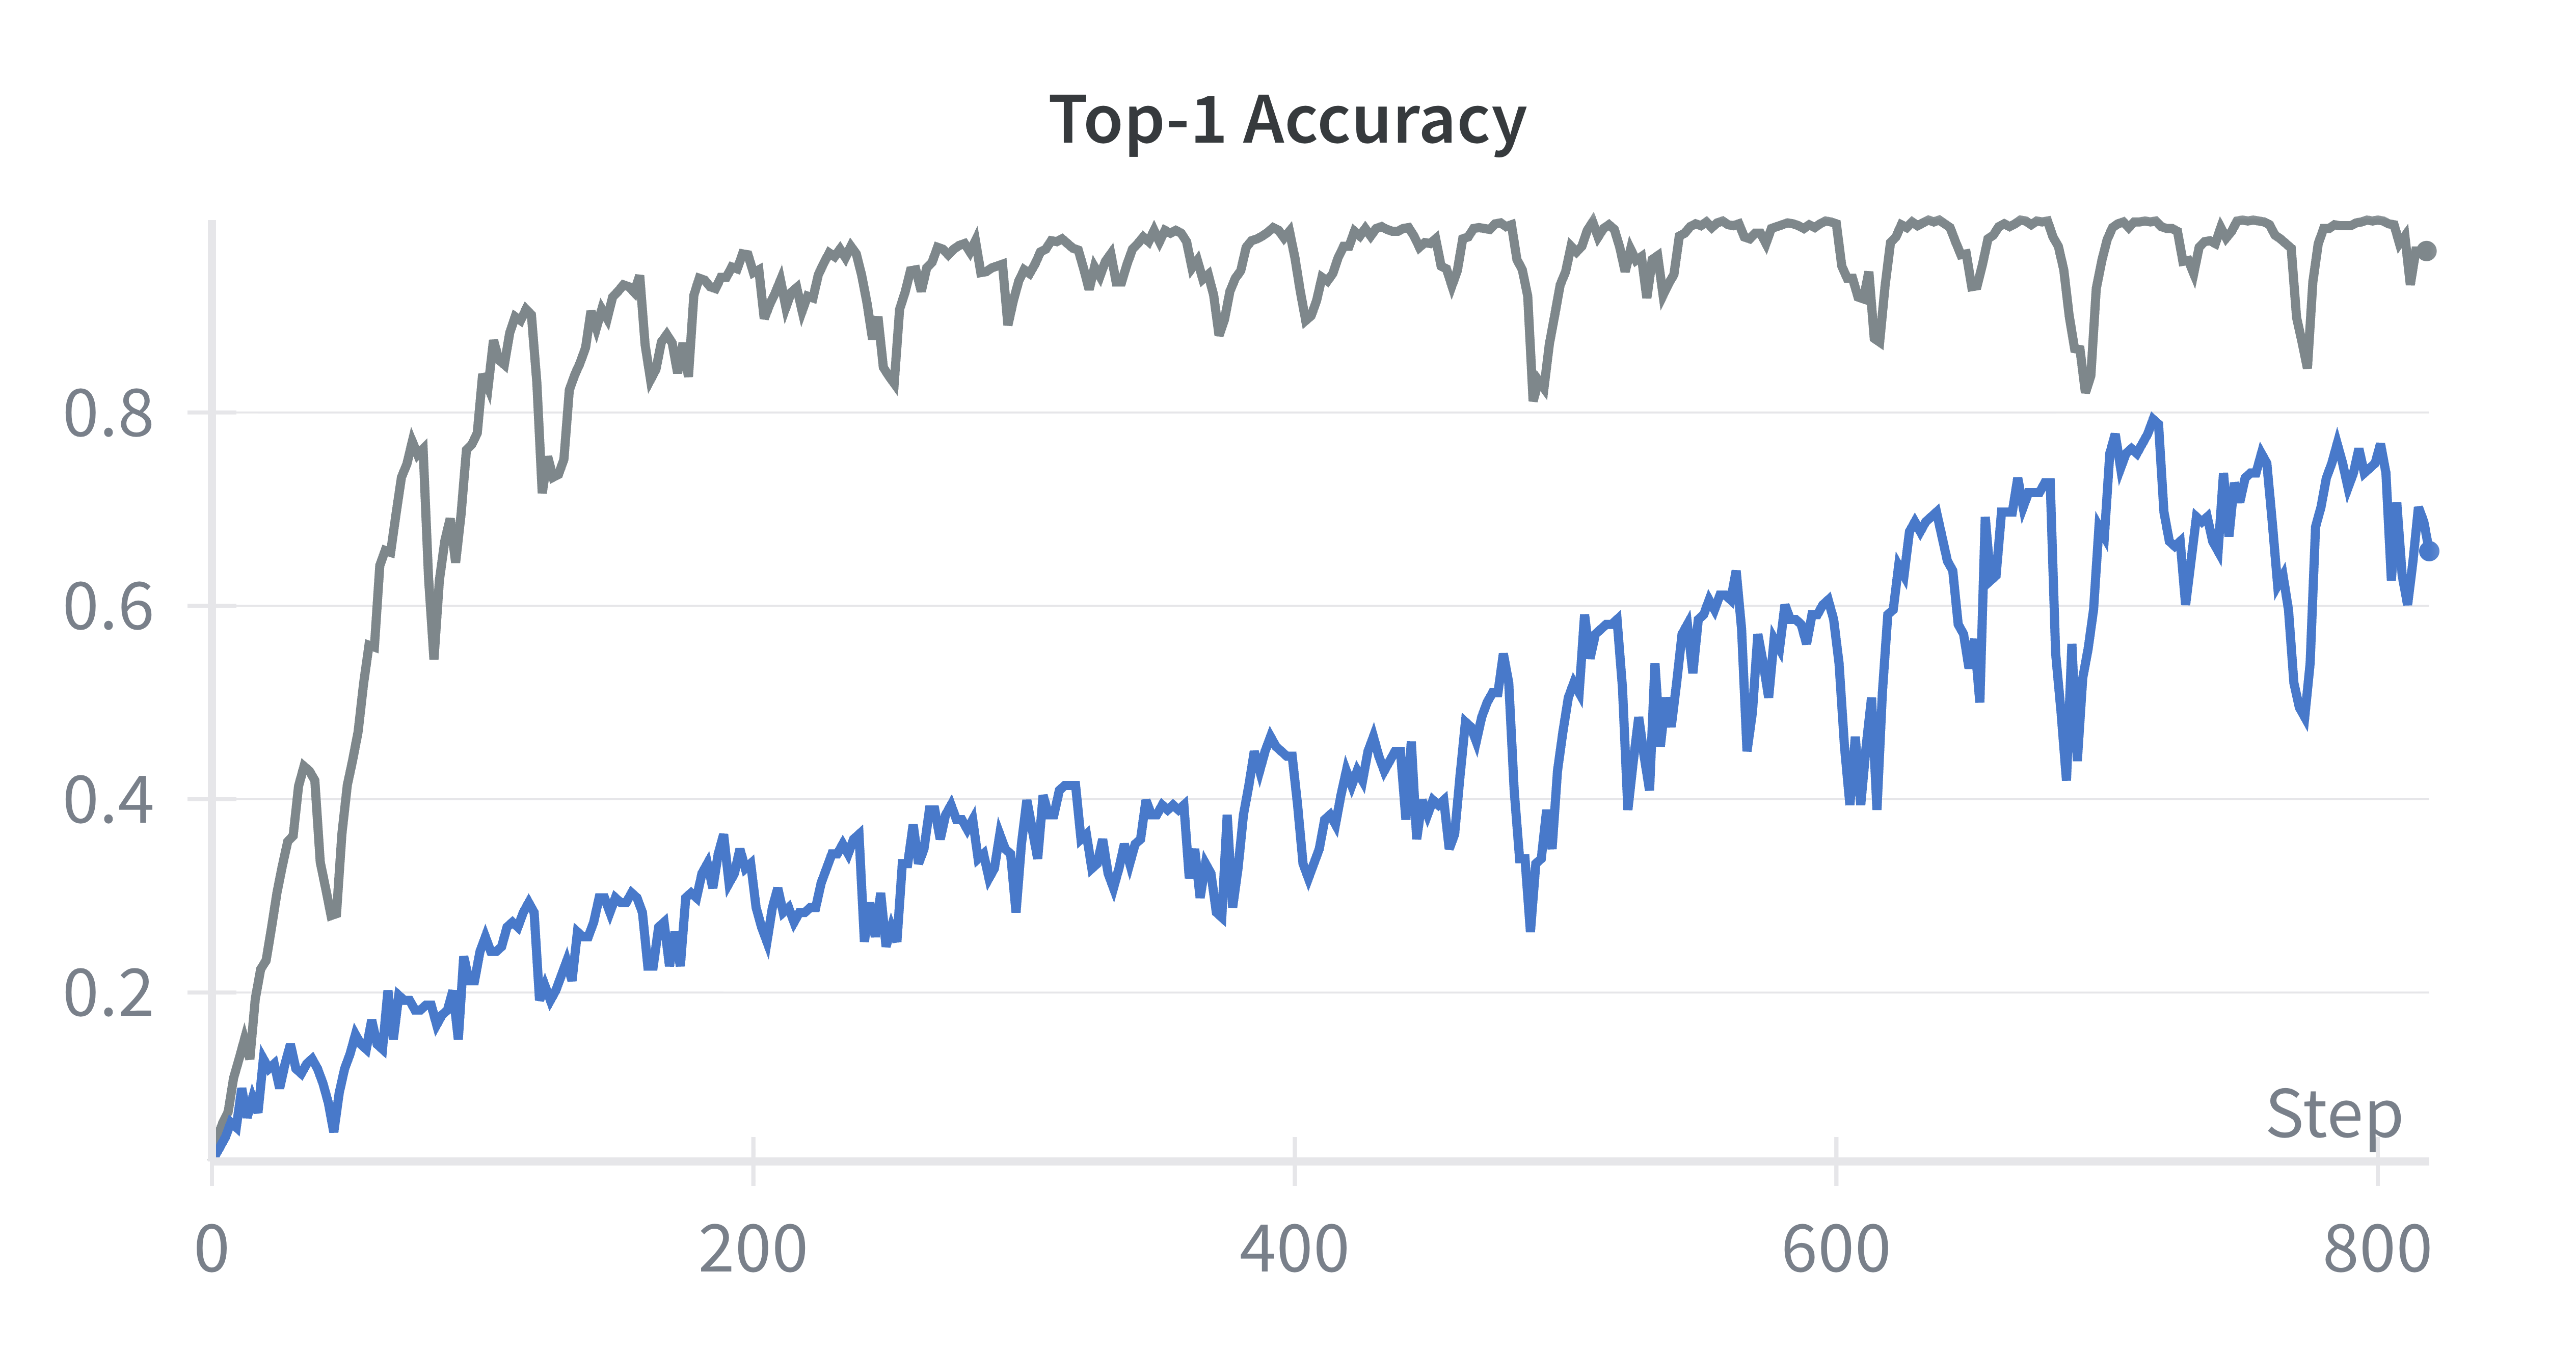
\includegraphics[width=\linewidth]{img_results/acc_noisy_alphanum.png}
      \subcaption{Alphanumeric keys}
  \end{minipage}
  \hfill
  \begin{minipage}{0.49\linewidth}
      \centering
      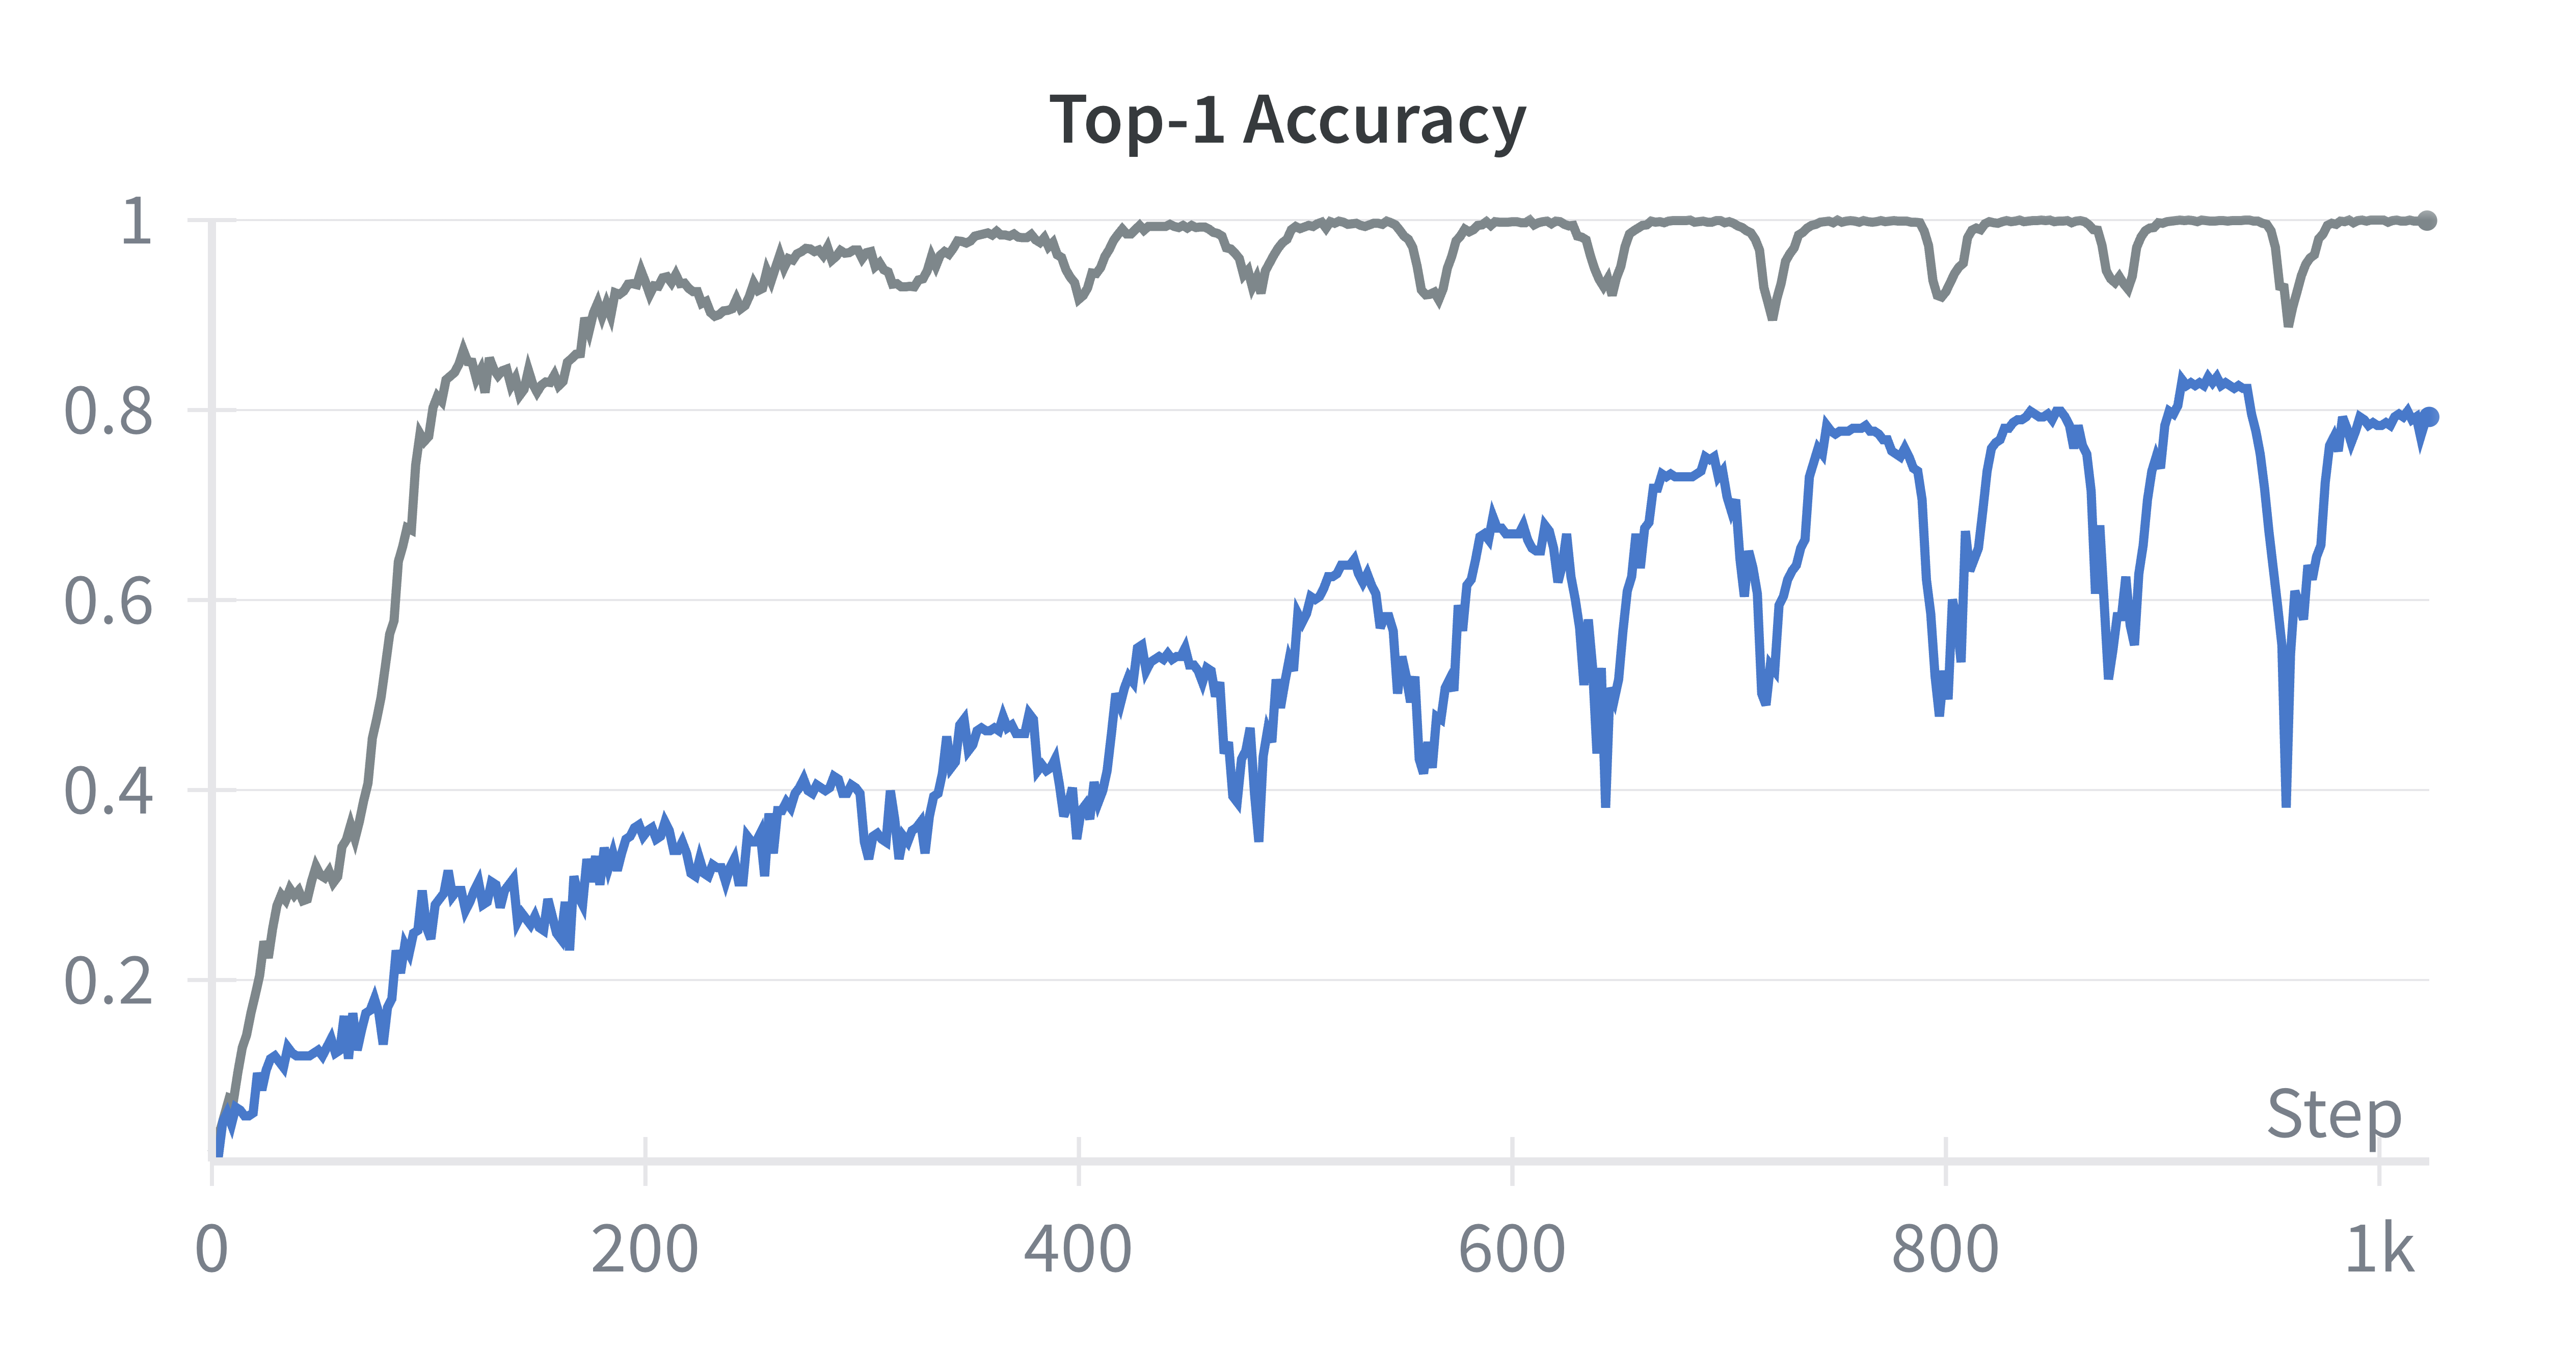
\includegraphics[width=\linewidth]{img_results/acc_noisy_all.png}
      \subcaption{All keys}
  \end{minipage}
  \caption{Training history of best CoAtNet-4 architecture on different sets of keys with background noise.}
  \label{fig:acc_noisy}
\end{figure}

Table~\ref{tab:topk_noisy_train} presents the top-$k$ accuracies for models trained on noisy recordings and evaluated on both clean and noisy subsets. While the Top-1 accuracy on the clean dataset shows a noticeable drop compared to the noisy evaluation, the Top-$k$ accuracies increase rapidly as \texttt{k} grows. This trend demonstrates that the correct key is frequently captured within the first few predictions, significantly reducing ambiguity and highlighting the potential of these models in practical reconstruction scenarios.

As part of the task, the training history was also assessed. As shown in Figure \ref{fig:acc_noisy}, the models adapted quickly to the training data, whereas alignment with the validation subset increased more slowly but steadily over time.


To further analyze classification performance and error patterns, confusion matrices (Figure \ref{fig:confusion_matrices_noisy} and \ref{fig:confusion_matrices_noisy_mac}) were generated for the best-performing models on both key sets. For each dataset, separate matrices were produced for predictions on clean and noisy recordings.

% \begin{figure}[h!]
%   \centering
%   % \begin{minipage}{0.49\linewidth}
%   %     \centering
%   %     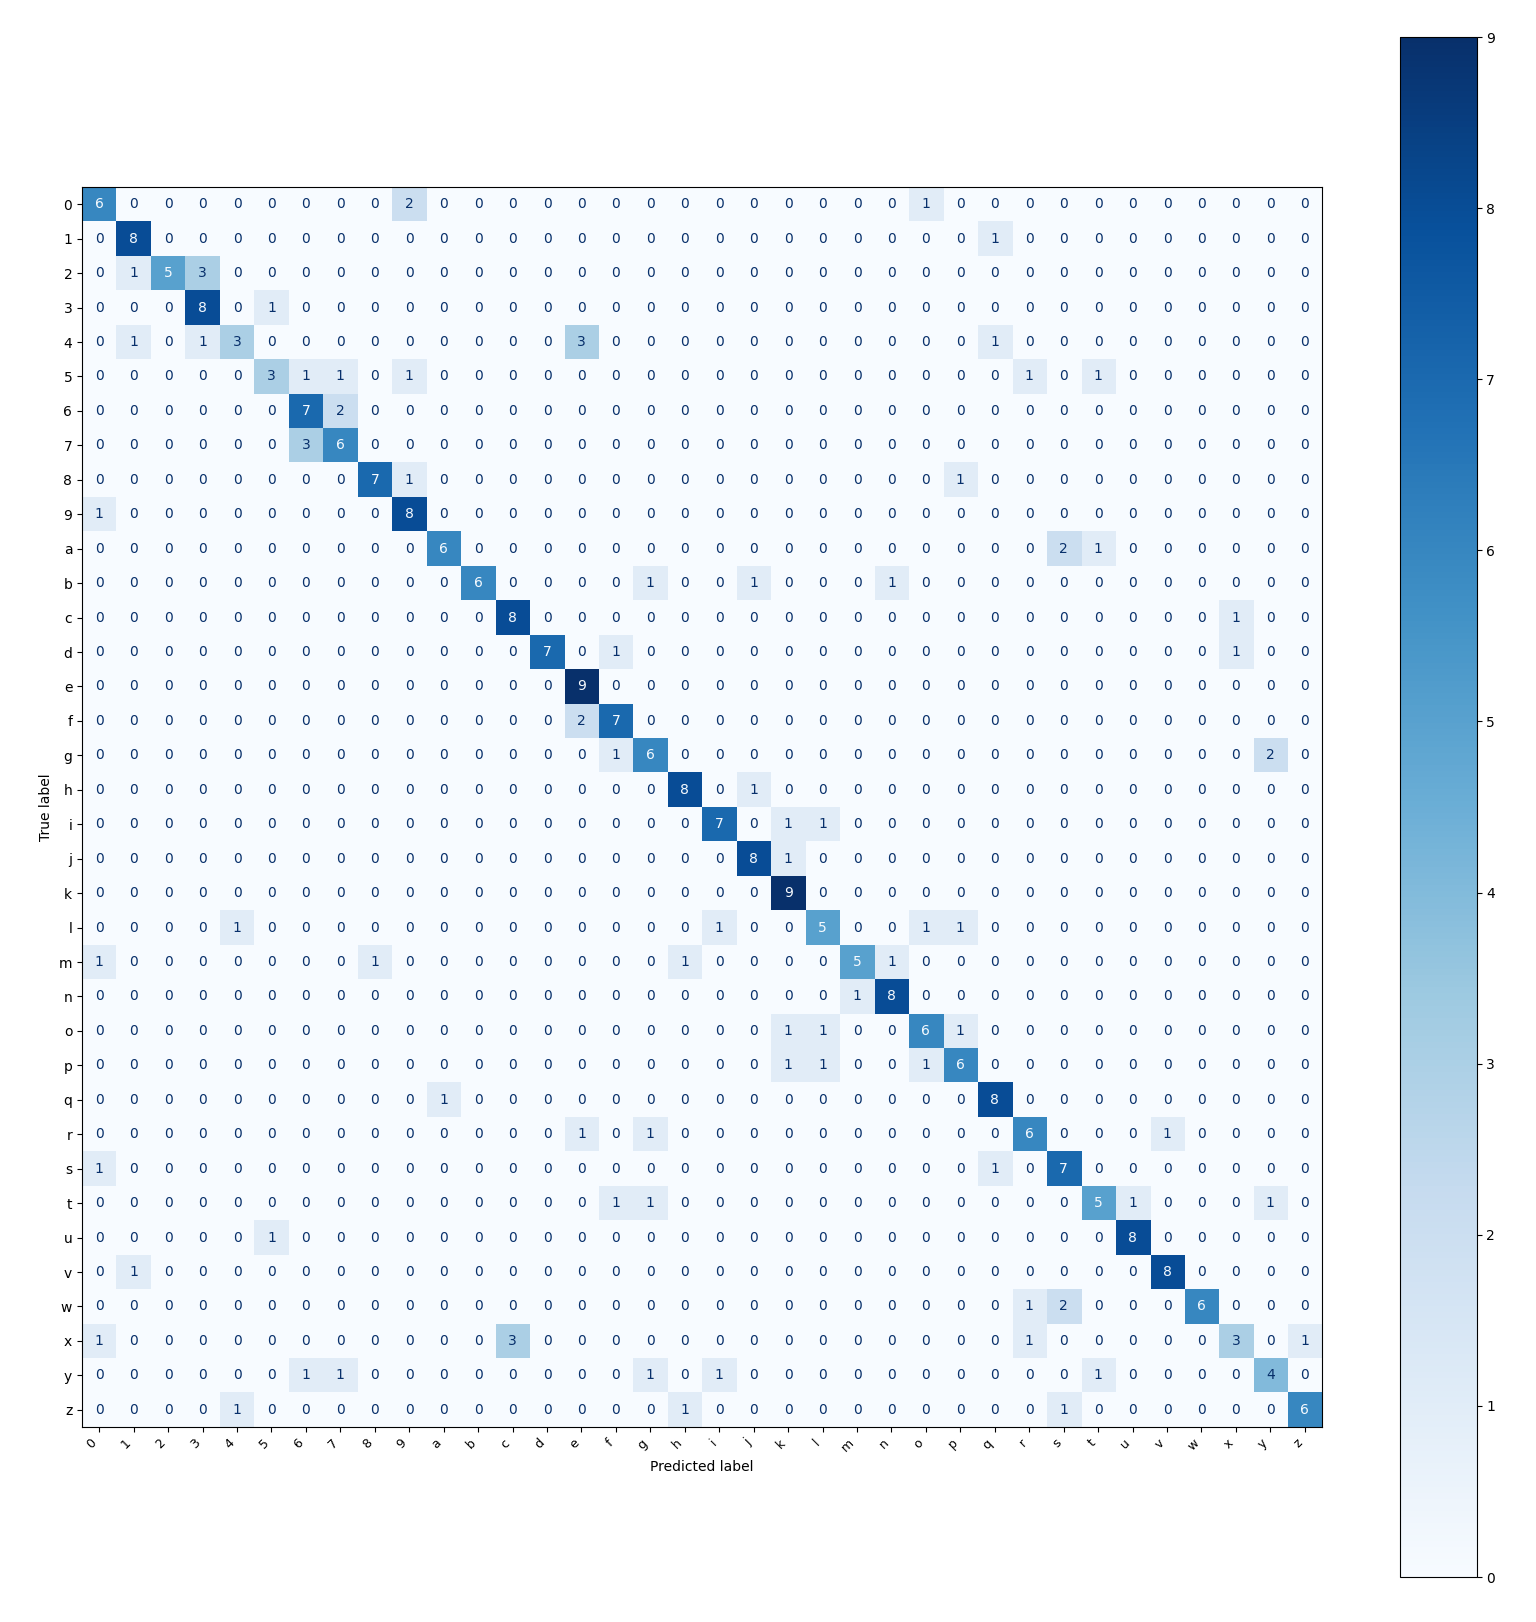
\includegraphics[width=\linewidth]{img_results/cm_noisy_alphanum_noisy.png}
%   %     \subcaption{}
%   % \end{minipage}
%   % \hfill
%   % \begin{minipage}{0.49\linewidth}
%   %     \centering
%   %     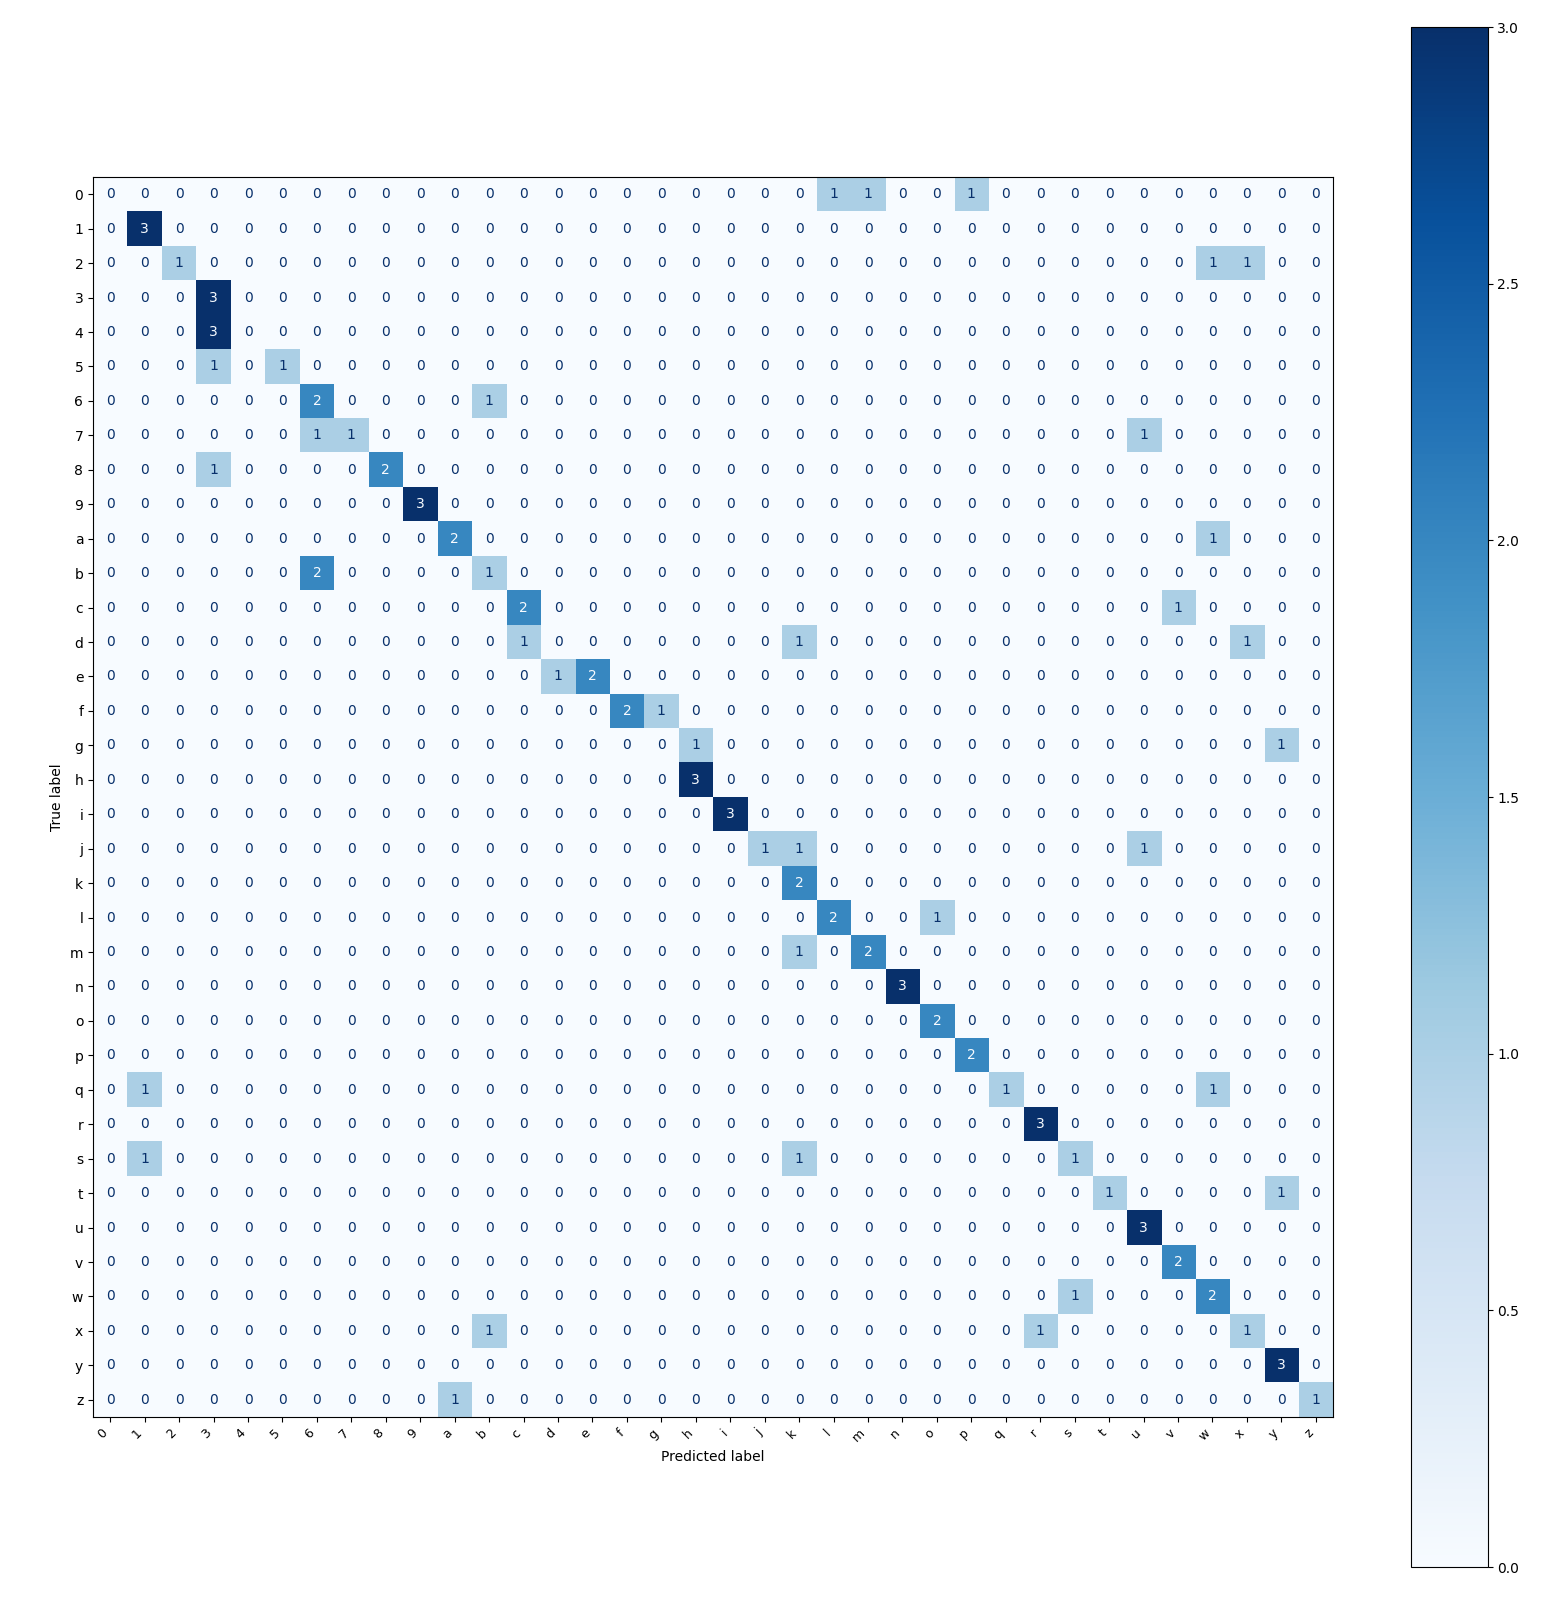
\includegraphics[width=\linewidth]{img_results/cm_noisy_alphanum_mac.png}
%   %     \subcaption{}
%   % \end{minipage}

%   \begin{minipage}{0.75\linewidth}
%       \centering
%       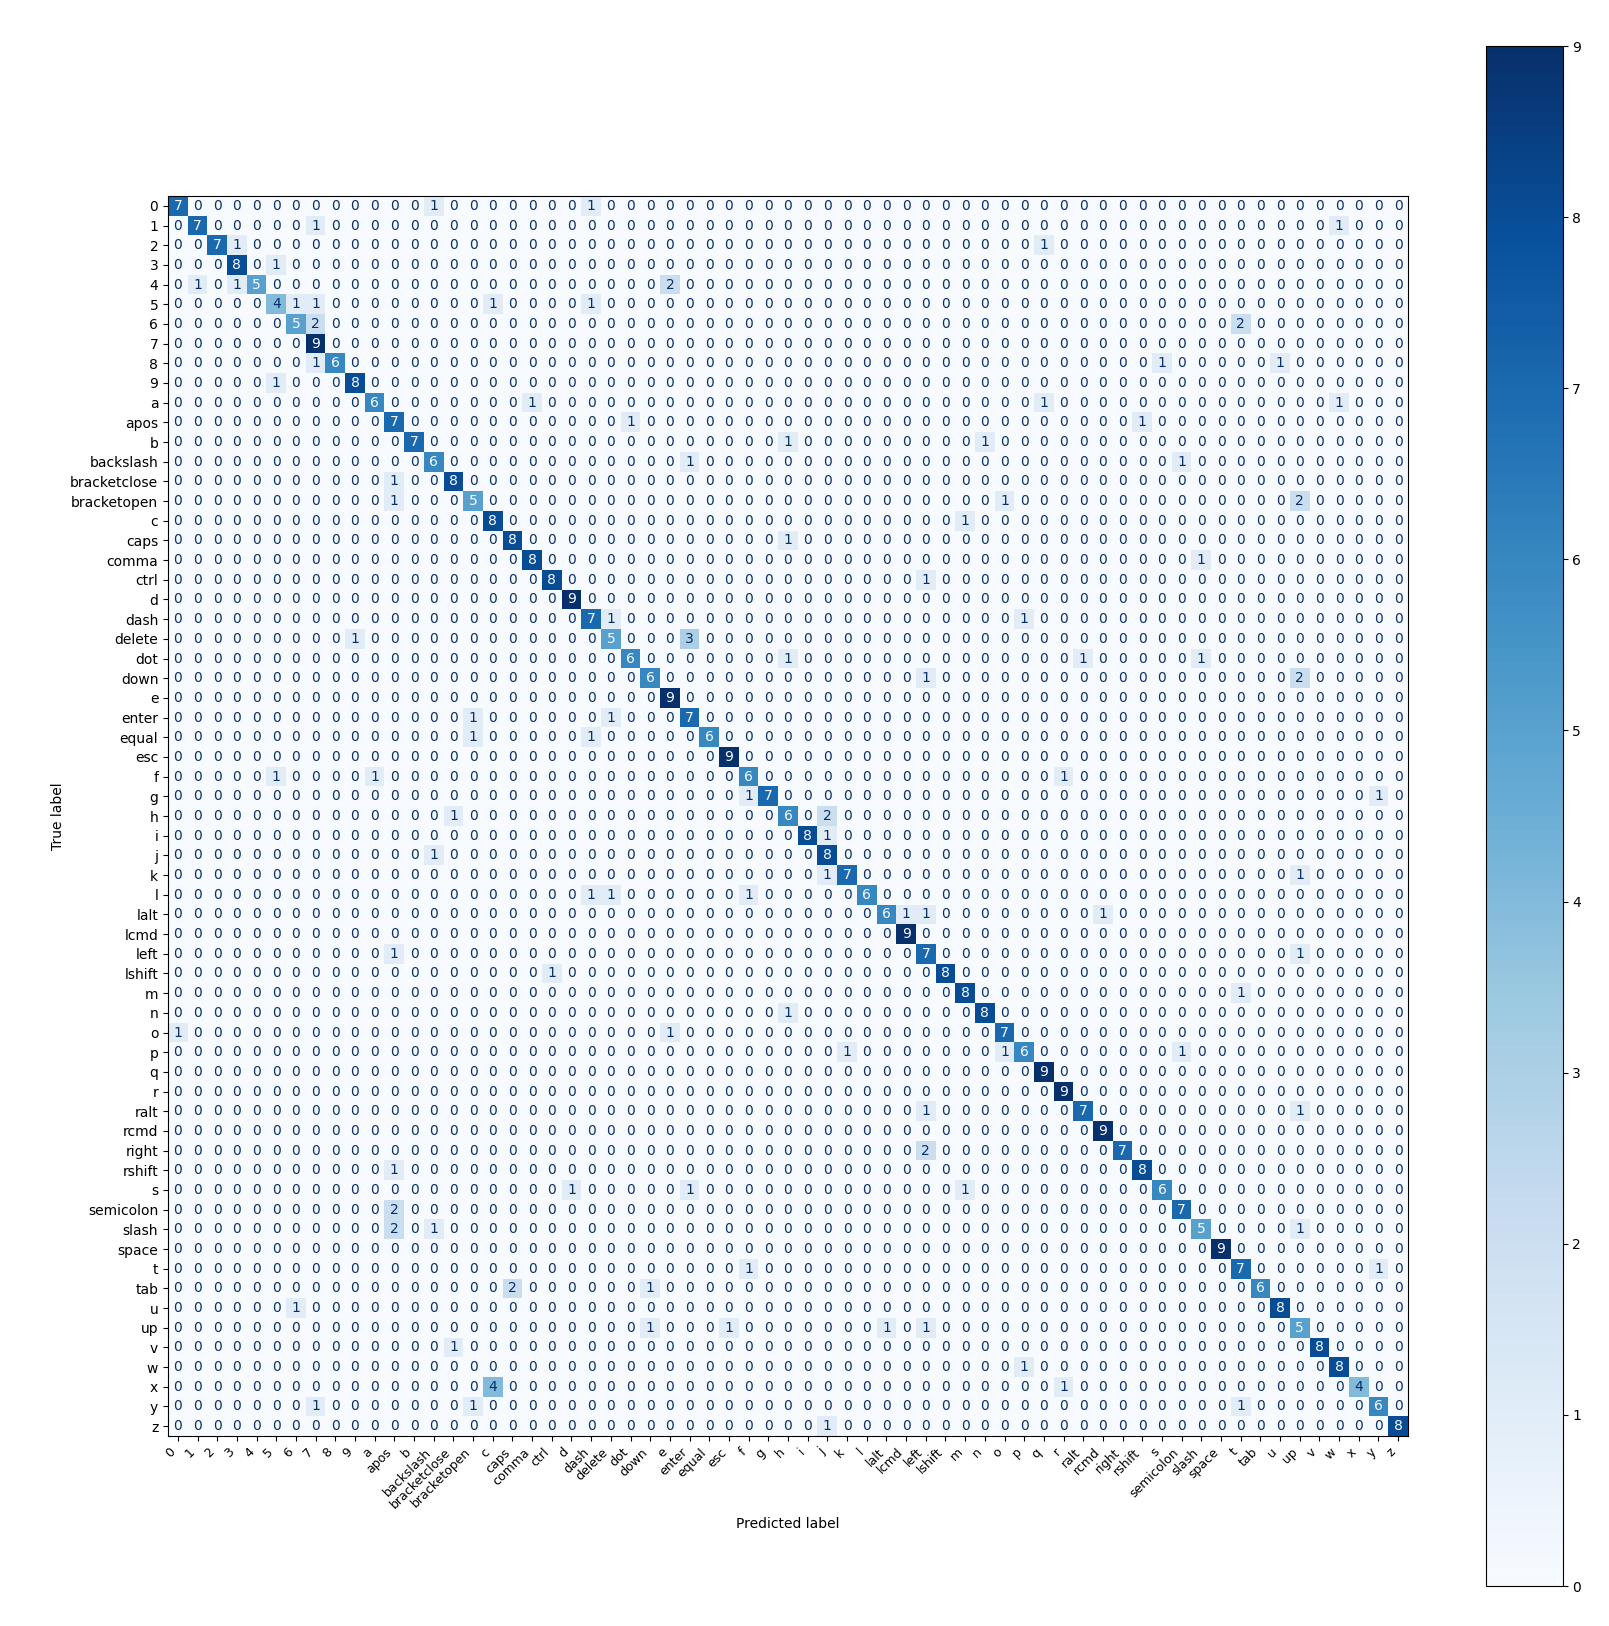
\includegraphics[width=\linewidth]{img_results/cm_noisy_all_noisy.png}
%       \subcaption{Noisy recordings}
%   \end{minipage}
%   \hfill
%   \begin{minipage}{0.75\linewidth}
%       \centering
%       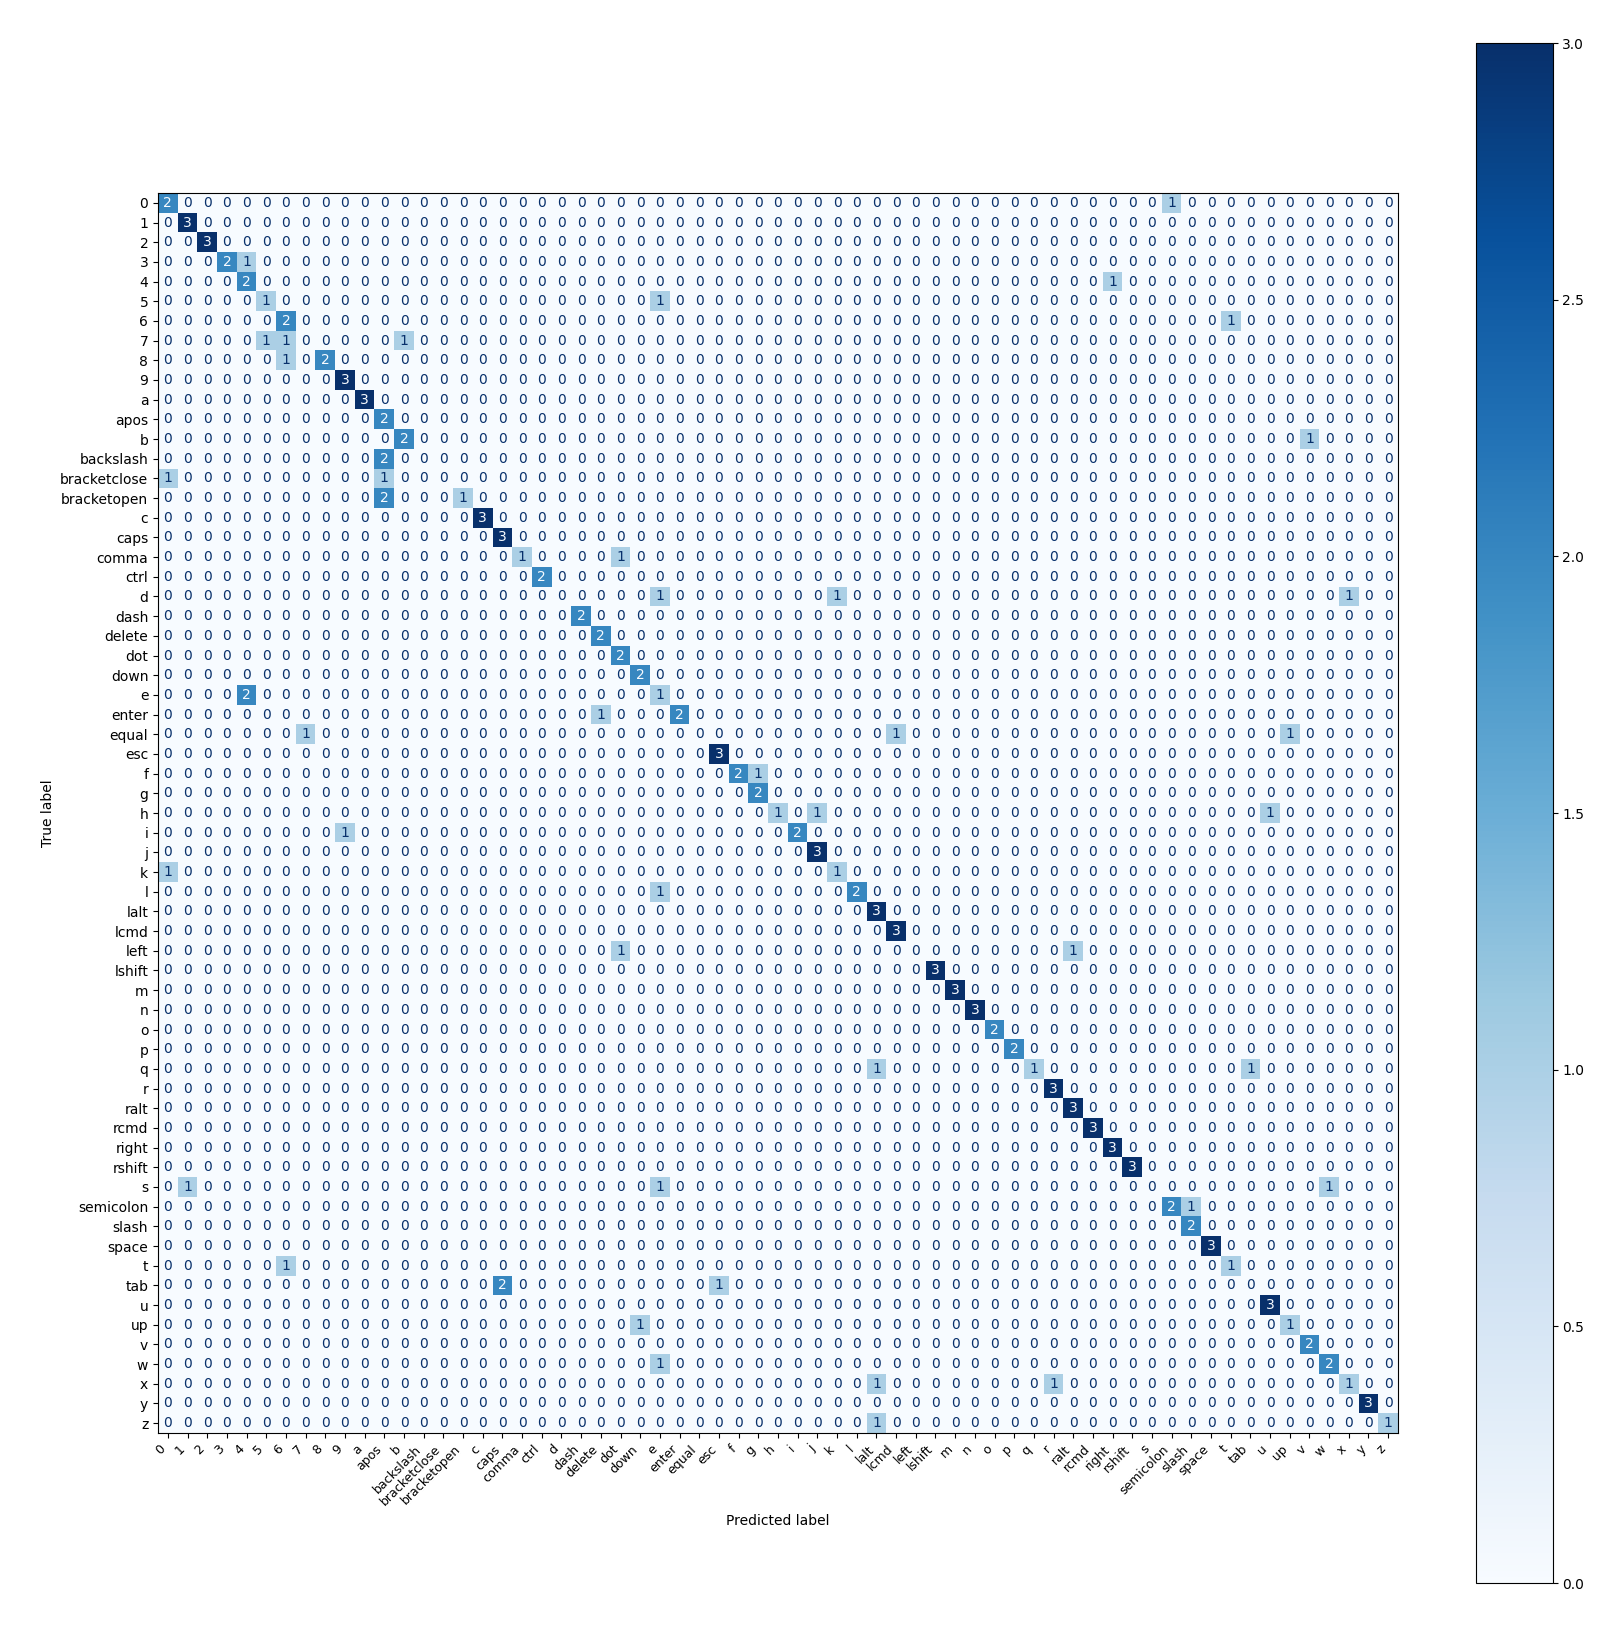
\includegraphics[width=\linewidth]{img_results/cm_noisy_all_mac.png}
%       \subcaption{Clean recordings}
%   \end{minipage}

%   \caption{Confusion matrices of the best CoAtNet-4 model trained with all keys on noisy data and evaluated on different audio recordings.}
%   \label{fig:confusion_matrices_noisy}
% \end{figure}

\begin{figure}[h!]
  \centering
  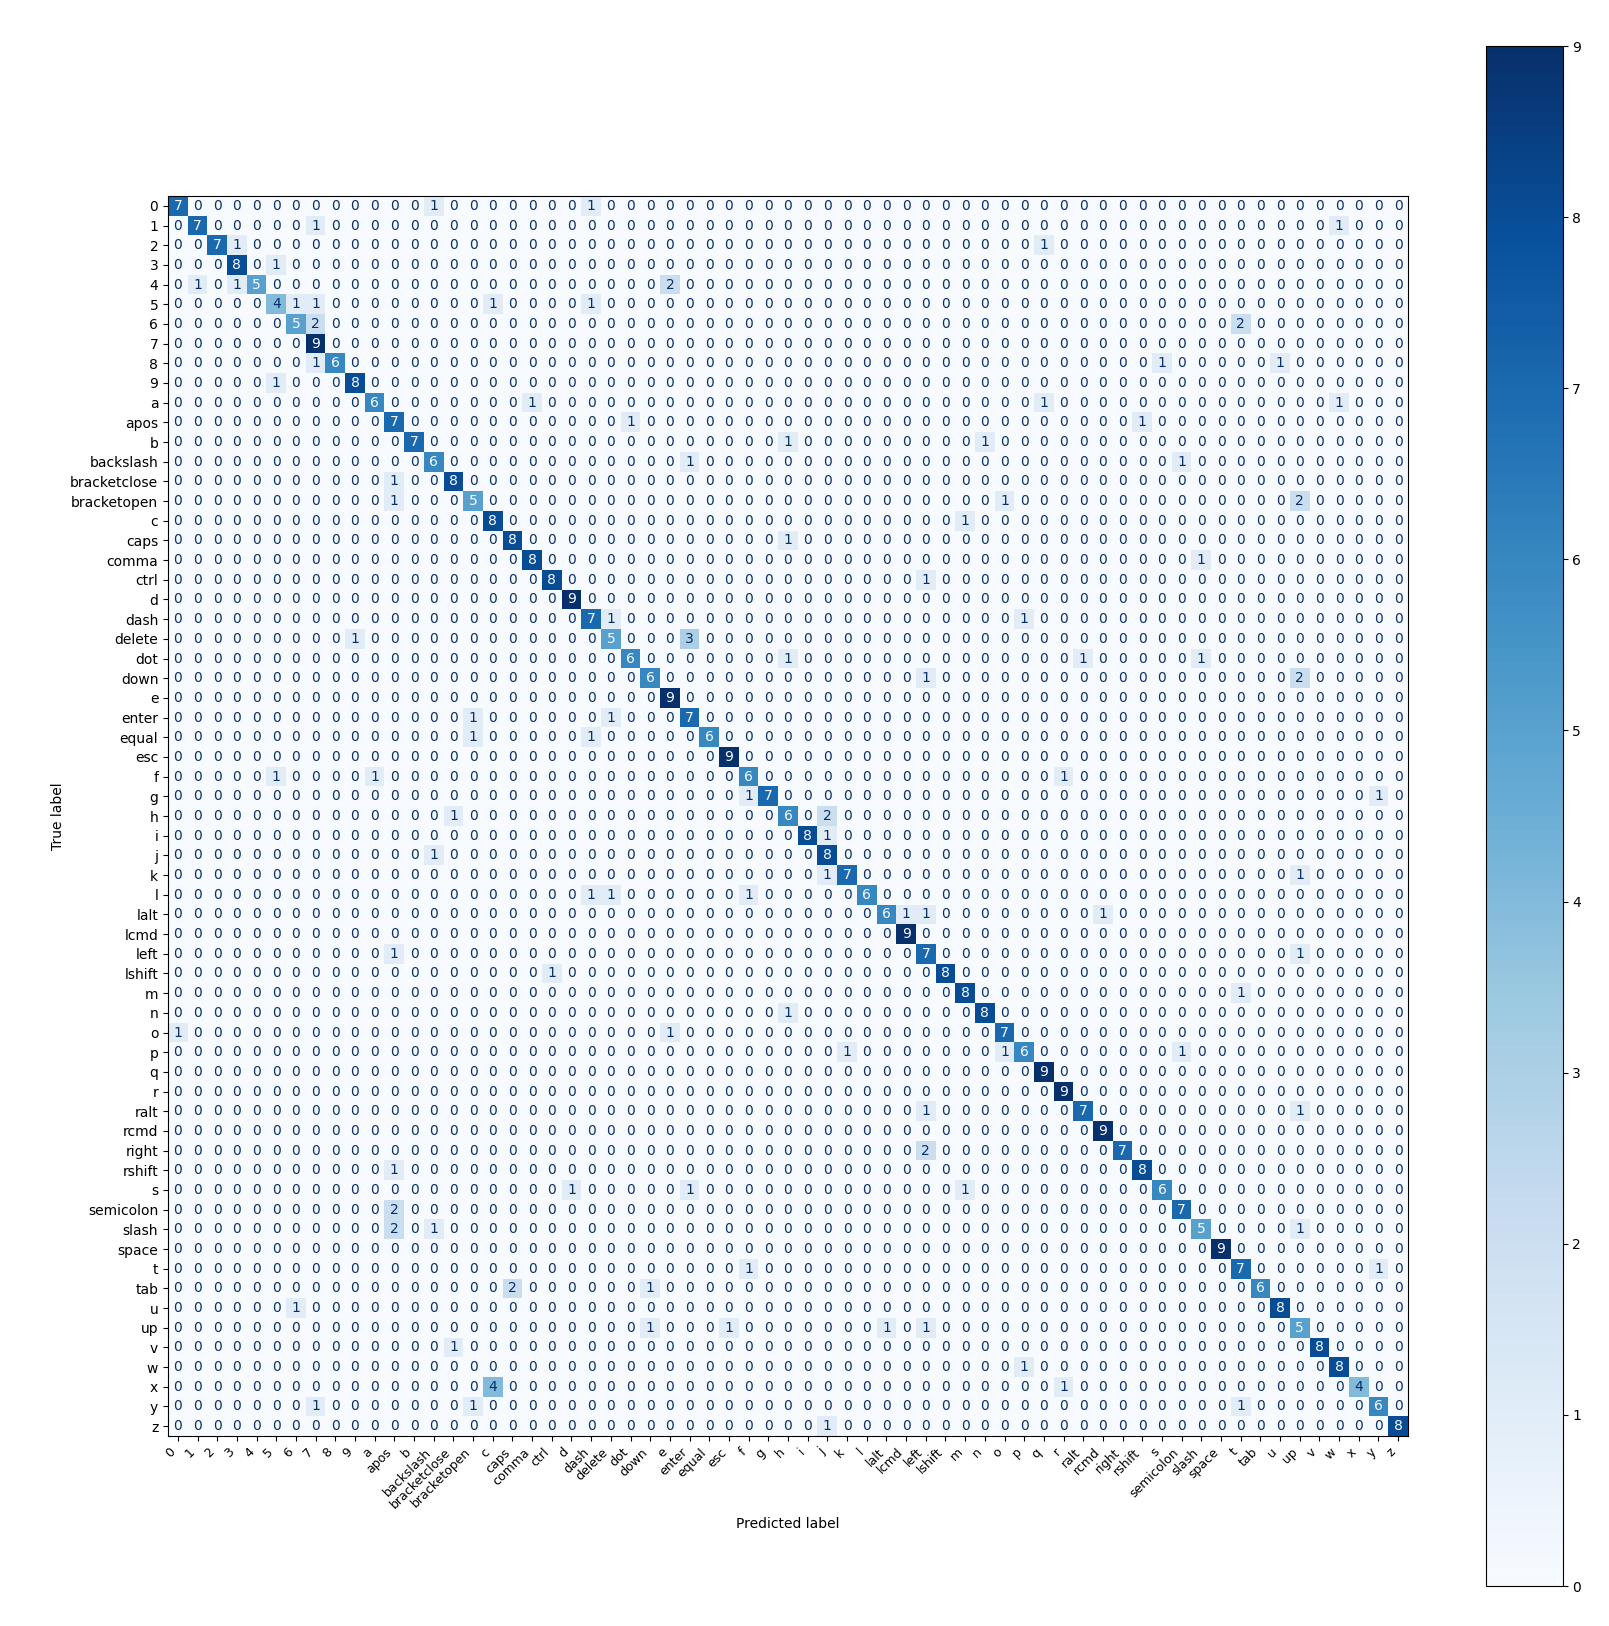
\includegraphics[width=\linewidth]{img_results/cm_noisy_all_noisy.png}
  % \subcaption{Noisy recordings}
  \caption{Confusion matrices of the best CoAtNet-4 model trained with all keys on noisy data and evaluated on noisy recordings.}
  \label{fig:confusion_matrices_noisy}
\end{figure}
\begin{figure}[h!]
  \centering
  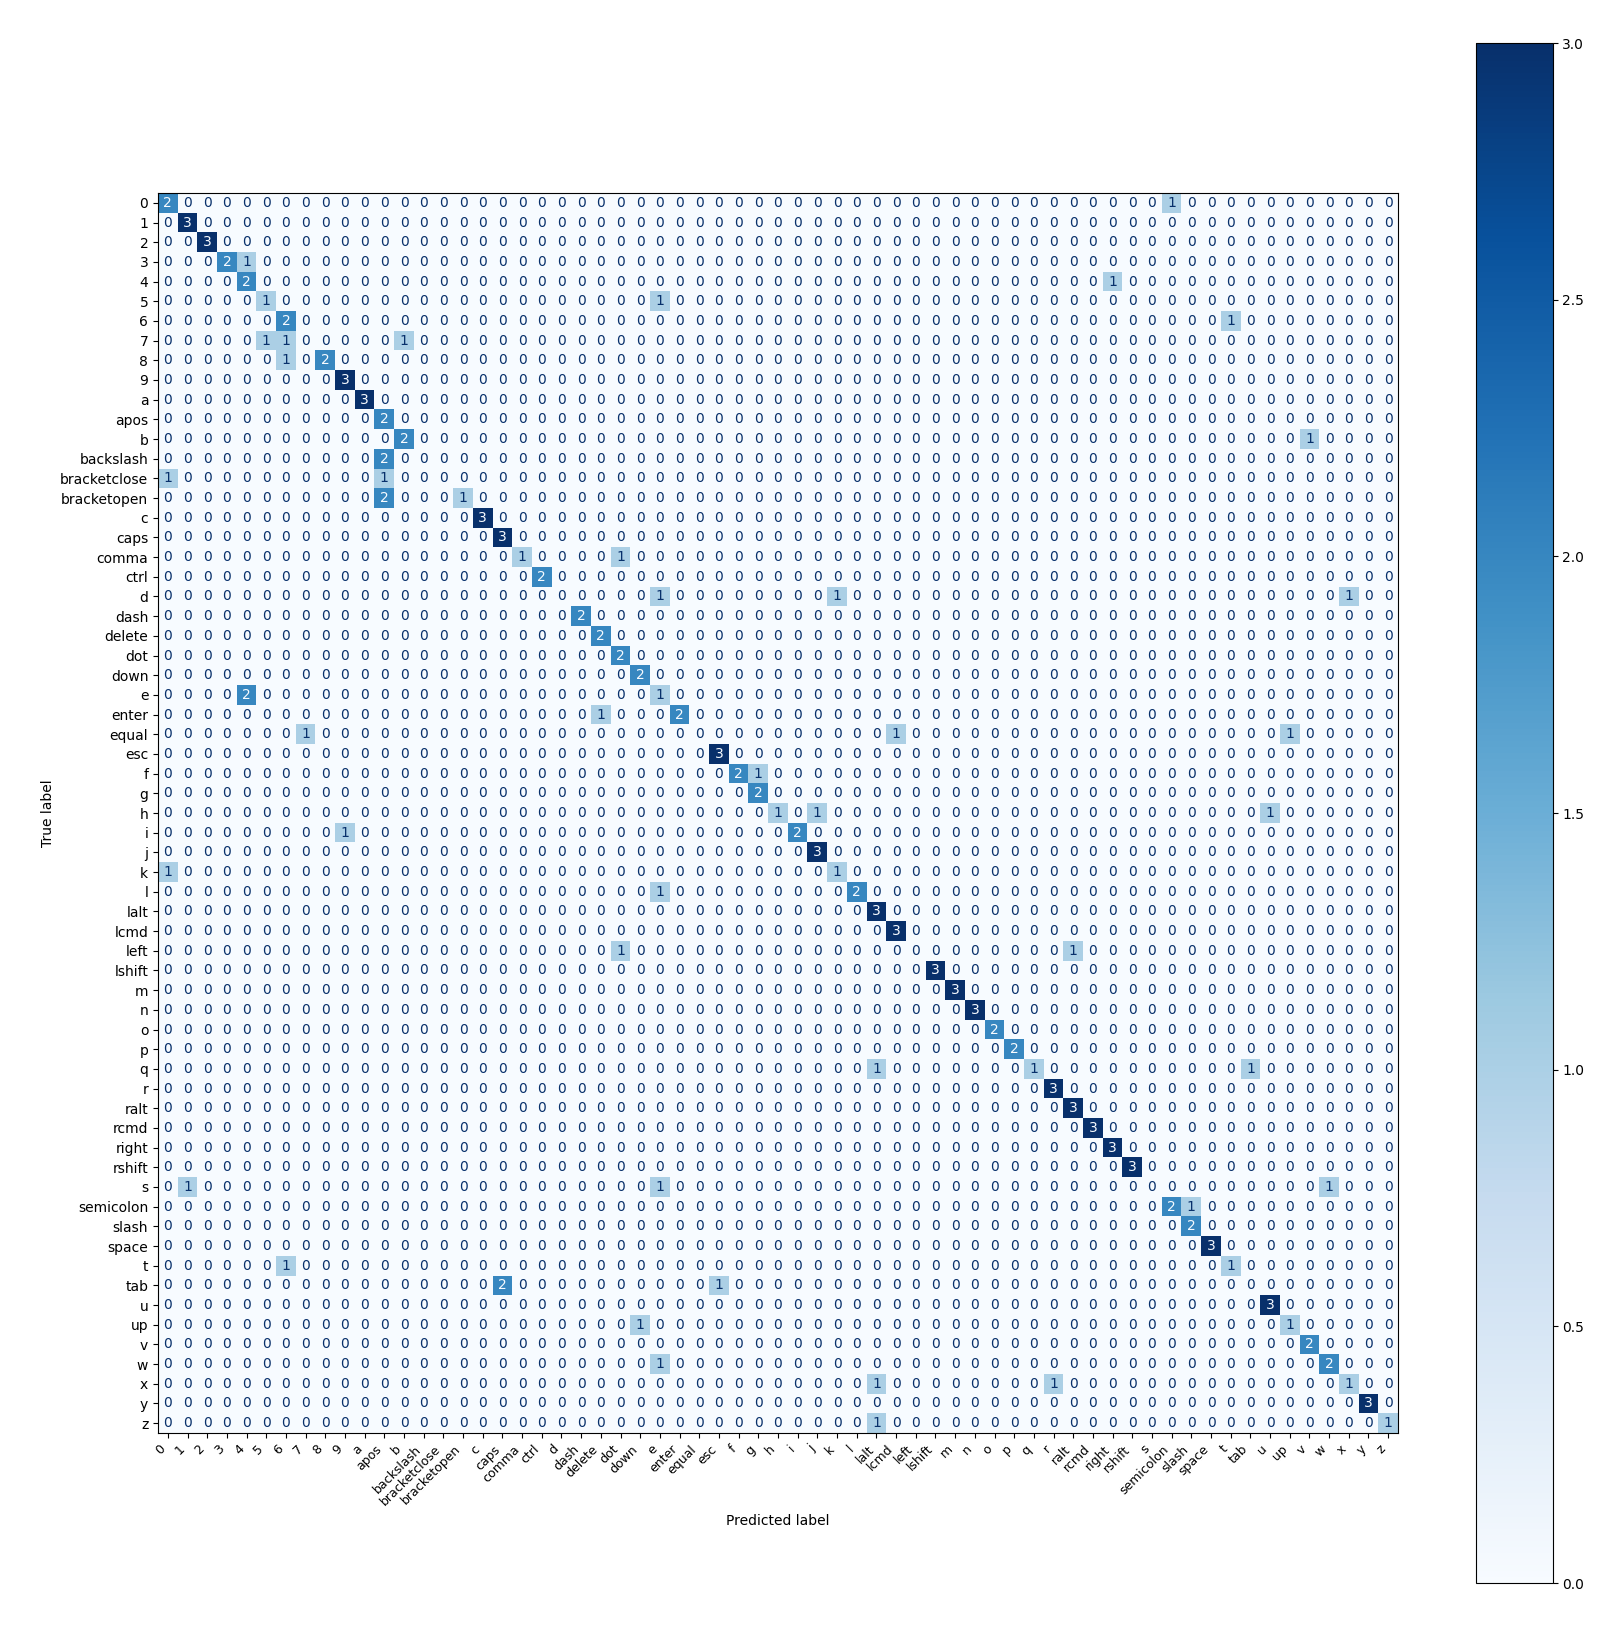
\includegraphics[width=\linewidth]{img_results/cm_noisy_all_mac.png}
  % \subcaption{Noisy recordings}
  \caption{Confusion matrices of the best CoAtNet-4 model trained with all keys on noisy data and evaluated on clean recordings.}
  \label{fig:confusion_matrices_noisy_mac}
\end{figure}

From these matrices, the same pattern can be observed: while the majority of recordings are classified correctly, some misclassifications occur, particularly between keys located close to each other on the keyboard, such as 6 and 7, w and s, or k and j.


\chapter{Conclusions}

This study investigated the feasibility and limitations of acoustic side-channel attacks for keystroke recognition using neural network architectures, including CoAtNet, MOAT, and Swin Transformer. Two experimental scenarios were considered: a controlled setting with clean, segmented public recordings, and a real-world simulation incorporating noisy and diverse acoustic environments. In both analyses, the impact of architectural choices, model scale, dataset composition, and post-processing strategies was evaluated, providing comprehensive information on model performance, robustness, and practical applicability.

In the controlled experiments on alphanumeric key presses, CoAtNet consistently achieved the highest accuracy, with medium- and large-scale variants achieving even 92.21\% overall accuracy. Notably, when evaluated on the dataset that is present in published works together with additional training data, CoAtNet achieved a state-of-the-art result of 95.23\% accuracy. MOAT demonstrated competitive results, often surpassing 88\% accuracy, with models using local attention slightly outperforming those with global attention. Swin Transformer, in contrast, lagged behind significantly, indicating limited suitability for this task under ideal conditions, proving strong effectiveness of convolutional layers. A clear correlation between model scale and performance was observed for CoAtNet, whereas MOAT’s performance was relatively insensitive to architectural size, and Swin Transformer exhibited weak performance regardless of configuration. Similar trends were observed in the scenario that included all keys from keyboard, although the increased number of classes and added complexity slightly reduced overall accuracy (by no more than 2\% with the best models). Top-$k$ accuracy analysis showed that even when the first prediction was incorrect, the correct key often appeared within the top few predictions, demonstrating that practical keystroke reconstruction remains feasible, particularly when combined with post-processing using large language models such as Gemini and GPT-OSS.

The real-world simulation highlighted the influence of noise and environmental variability on model performance. When trained on the full custom dataset, including both clean and noisy recordings, larger architectures consistently outperformed smaller ones, with clean recordings remaining substantially easier to predict than noisy subsets. Knowledge transfer experiments revealed a strong asymmetry: models trained exclusively on clean recordings failed to generalize to noisy conditions, whereas models trained on noisy data generalized well to clean recordings with only modest performance drops. Furthermore, models trained on the full key set generally achieved higher accuracy than those trained on only alphanumeric keys, underscoring the benefits of exposing networks to more diverse datasets.

In summary, the results demonstrate that acoustic side-channel attacks can be highly effective under ideal conditions, but their performance in realistic, noisy environments depends strongly on the diversity and quality of the training data. Perfectly clean conditions are rare in everyday situations, which considerably reduces the practical risk of such attacks. The study highlights the importance of model architecture and scale: larger and well-regularized models consistently achieve the best predictive performance, yet their effectiveness is tied to the specificity of the training setup. Exposure to heterogeneous and noisy recordings improves generalization, allowing models to maintain reasonable accuracy even when faced with acoustic disturbances. Post-processing with large language models further enhances reconstruction by leveraging semantic context, but this improvement primarily reflects general language patterns rather than sensitive, case-specific information, such as passwords, which remain more difficult to predict. Despite these advances, certain keys are inherently more prone to misclassification due to acoustic similarity or physical proximity on the keyboard, underscoring intrinsic limitations of audio-based keystroke recognition. Overall, these findings provide a comprehensive view of the potential and constraints of neural-network-based acoustic attacks, while also informing practical defenses, such as noise injection, hardware modifications, or keyboard layout adjustments, to mitigate risk in realistic scenarios.

\chapter{Future Work}

\printbibliography

\section*{Acknowledgments}

This research was carried out with the support of the High Performance Computing Center at Faculty of Mathematics and Information Science Warsaw University of Technology.

\newpage

\chapter*{Appendix}

\section*{Controlled Setting}

\begin{table}[ht]
\centering
\caption{Top-$k$ accuracies of models on the publicly available datasets with alphanumeric keys.}
\begin{adjustbox}{max width=\textwidth}
\begin{tabular}{c|c|c|cccccc}
\hline
\textbf{Model} & \textbf{Architecture} & \textbf{Window} & \multicolumn{6}{c}{\textbf{Accuracy (\%)}} \\
\cline{4-9}
 & \textbf{No.} & \textbf{Size} & \textbf{Top-1} & \textbf{Top-2} & \textbf{Top-3} & \textbf{Top-4} & \textbf{Top-5} & \textbf{Top-10} \\
\hline
CoAtNet & 3 & - & \textbf{92.21} & 96.57 & 97.82 & 98.29 & 98.75 & 99.53 \\
CoAtNet & 4 & - & 90.65 & \textbf{97.20} & \textbf{98.13} & \textbf{98.75} & \textbf{98.91} & 99.38 \\
MOAT & 2 & 16 & 88.16 & 95.48 & 97.04 & 97.66 & 98.75 & \textbf{99.69} \\
MOAT & 4 & 8 & 86.60 & 94.70 & 97.20 & 97.98 & 98.29 & 99.38 \\
MOAT & 1 & 8 & 86.29 & 93.93 & 97.04 & 97.66 & 98.29 & 99.07 \\
MOAT & 3 & - & 85.98 & 94.39 & 96.42 & 98.13 & 98.91 & 99.22 \\
MOAT & 4 & 16 & 85.67 & 94.86 & 96.73 & 97.51 & 98.13 & 99.53 \\
CoAtNet & 1 & - & 84.27 & 92.37 & 95.48 & 97.04 & 98.44 & 99.07 \\
CoAtNet & 2 & - & 83.64 & 92.52 & 94.70 & 96.73 & 97.82 & 99.53 \\
MOAT & 2 & - & 83.33 & 92.83 & 96.11 & 97.51 & 98.60 & 99.38 \\
MOAT & 4 & - & 82.71 & 93.77 & 96.88 & 98.44 & 98.60 & 99.53 \\
MOAT & 3 & 16 & 82.09 & 92.06 & 95.48 & 96.88 & 97.98 & 99.53 \\
MOAT & 1 & - & 80.06 & 91.28 & 95.48 & 96.57 & 97.66 & 98.91 \\
SwinTransformer & 3 & 8 & 55.30 & 71.81 & 78.50 & 84.27 & 88.47 & 95.02 \\
SwinTransformer & 2 & 4 & 53.89 & 70.25 & 77.26 & 83.64 & 87.38 & 93.93 \\
SwinTransformer & 4 & 16 & 23.99 & 36.60 & 44.55 & 50.62 & 57.48 & 75.39 \\
SwinTransformer & 1 & 4 & 38.47 & 52.96 & 64.49 & 70.09 & 76.79 & 90.34 \\
\hline
\end{tabular}
\end{adjustbox}
\end{table}
\begin{table}[h!]
\centering
\caption{Top-$k$ accuracies of models on the publicly available datasets with all keys.}
\begin{adjustbox}{max width=\textwidth}
\begin{tabular}{c|c|c|cccccc}
\hline
\textbf{Model} & \textbf{Architecture} & \textbf{Window} & \multicolumn{6}{c}{\textbf{Accuracy (\%)}} \\
\cline{4-9}
 & \textbf{No.} & \textbf{Size} & \textbf{Top-1} & \textbf{Top-2} & \textbf{Top-3} & \textbf{Top-4} & \textbf{Top-5} & \textbf{Top-10} \\
\hline
CoAtNet & 3 & - & \textbf{90.94} & \textbf{97.02} & \textbf{98.19} & 98.58 & 98.84 & 99.48 \\
CoAtNet & 4 & - & 90.82 & 96.64 & 97.80 & \textbf{98.58} & \textbf{98.97} & 99.35 \\
MOAT & 3 & - & 89.65 & 96.38 & 98.06 & 98.45 & \textbf{98.58} & \textbf{99.61} \\
MOAT & 1 & - & 87.71 & 94.70 & 97.41 & 98.32 & 98.84 & 99.35 \\
MOAT & 3 & 8 & 86.03 & 94.44 & 96.64 & 97.67 & 98.06 & 98.84 \\
MOAT & 1 & 8 & 85.77 & 93.79 & 96.38 & 97.67 & 98.19 & 99.09 \\
MOAT & 2 & 16 & 84.48 & 93.92 & 95.73 & 96.90 & 98.06 & 99.09 \\
CoAtNet & 1 & - & 83.31 & 92.76 & 95.86 & 97.41 & 98.19 & 99.35 \\
CoAtNet & 2 & - & 78.78 & 91.33 & 93.66 & 95.73 & 97.28 & 98.84 \\
SwinTransformer & 3 & 8 & 58.47 & 74.26 & 80.47 & 84.48 & 87.32 & 93.79 \\
SwinTransformer & 2 & 4 & 54.59 & 67.92 & 74.77 & 80.34 & 83.70 & 93.40 \\
SwinTransformer & 4 & 16 & 49.29 & 64.81 & 74.77 & 79.30 & 81.63 & 90.82 \\
SwinTransformer & 1 & 4 & 39.07 & 55.63 & 65.07 & 71.93 & 76.84 & 87.45 \\
\hline
\end{tabular}
\end{adjustbox}
\end{table}


\begin{figure}[H]
\centering

\begin{subfigure}{\linewidth}
    \centering
    \begin{minipage}{0.49\linewidth}
        \centering
        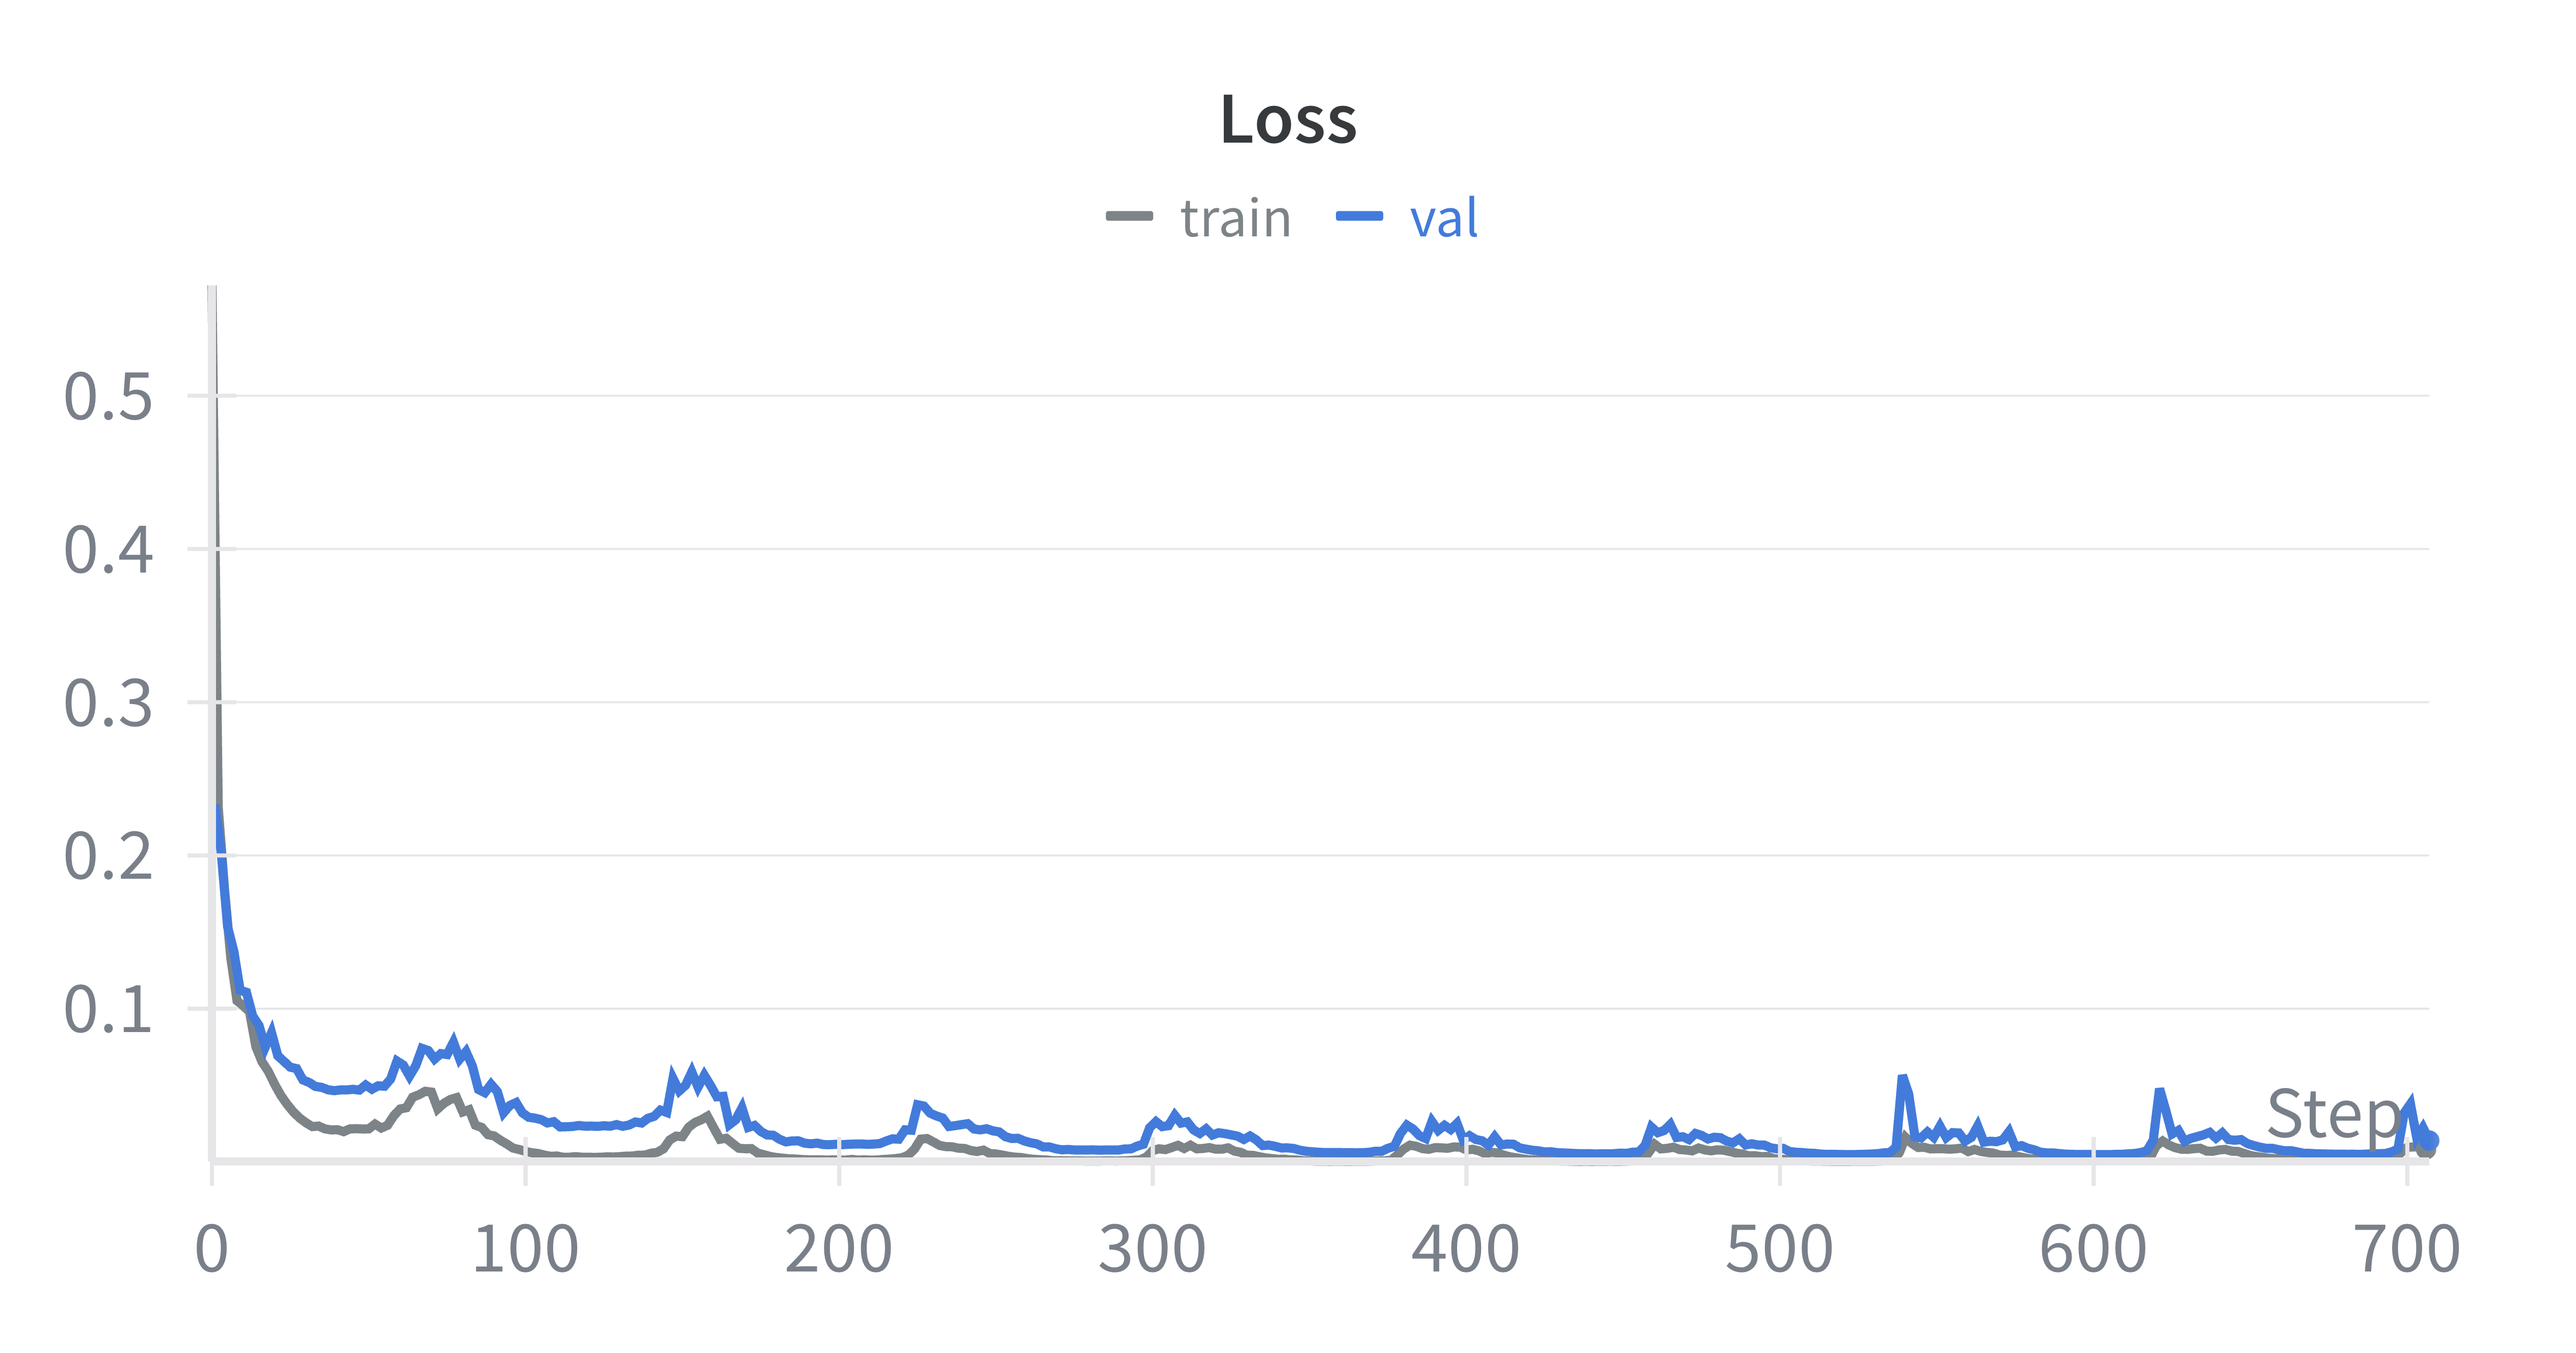
\includegraphics[width=\linewidth]{img_appendix/loss_all_moat_alphanum.png}
    \end{minipage}
    \hfill
    \begin{minipage}{0.49\linewidth}
        \centering
        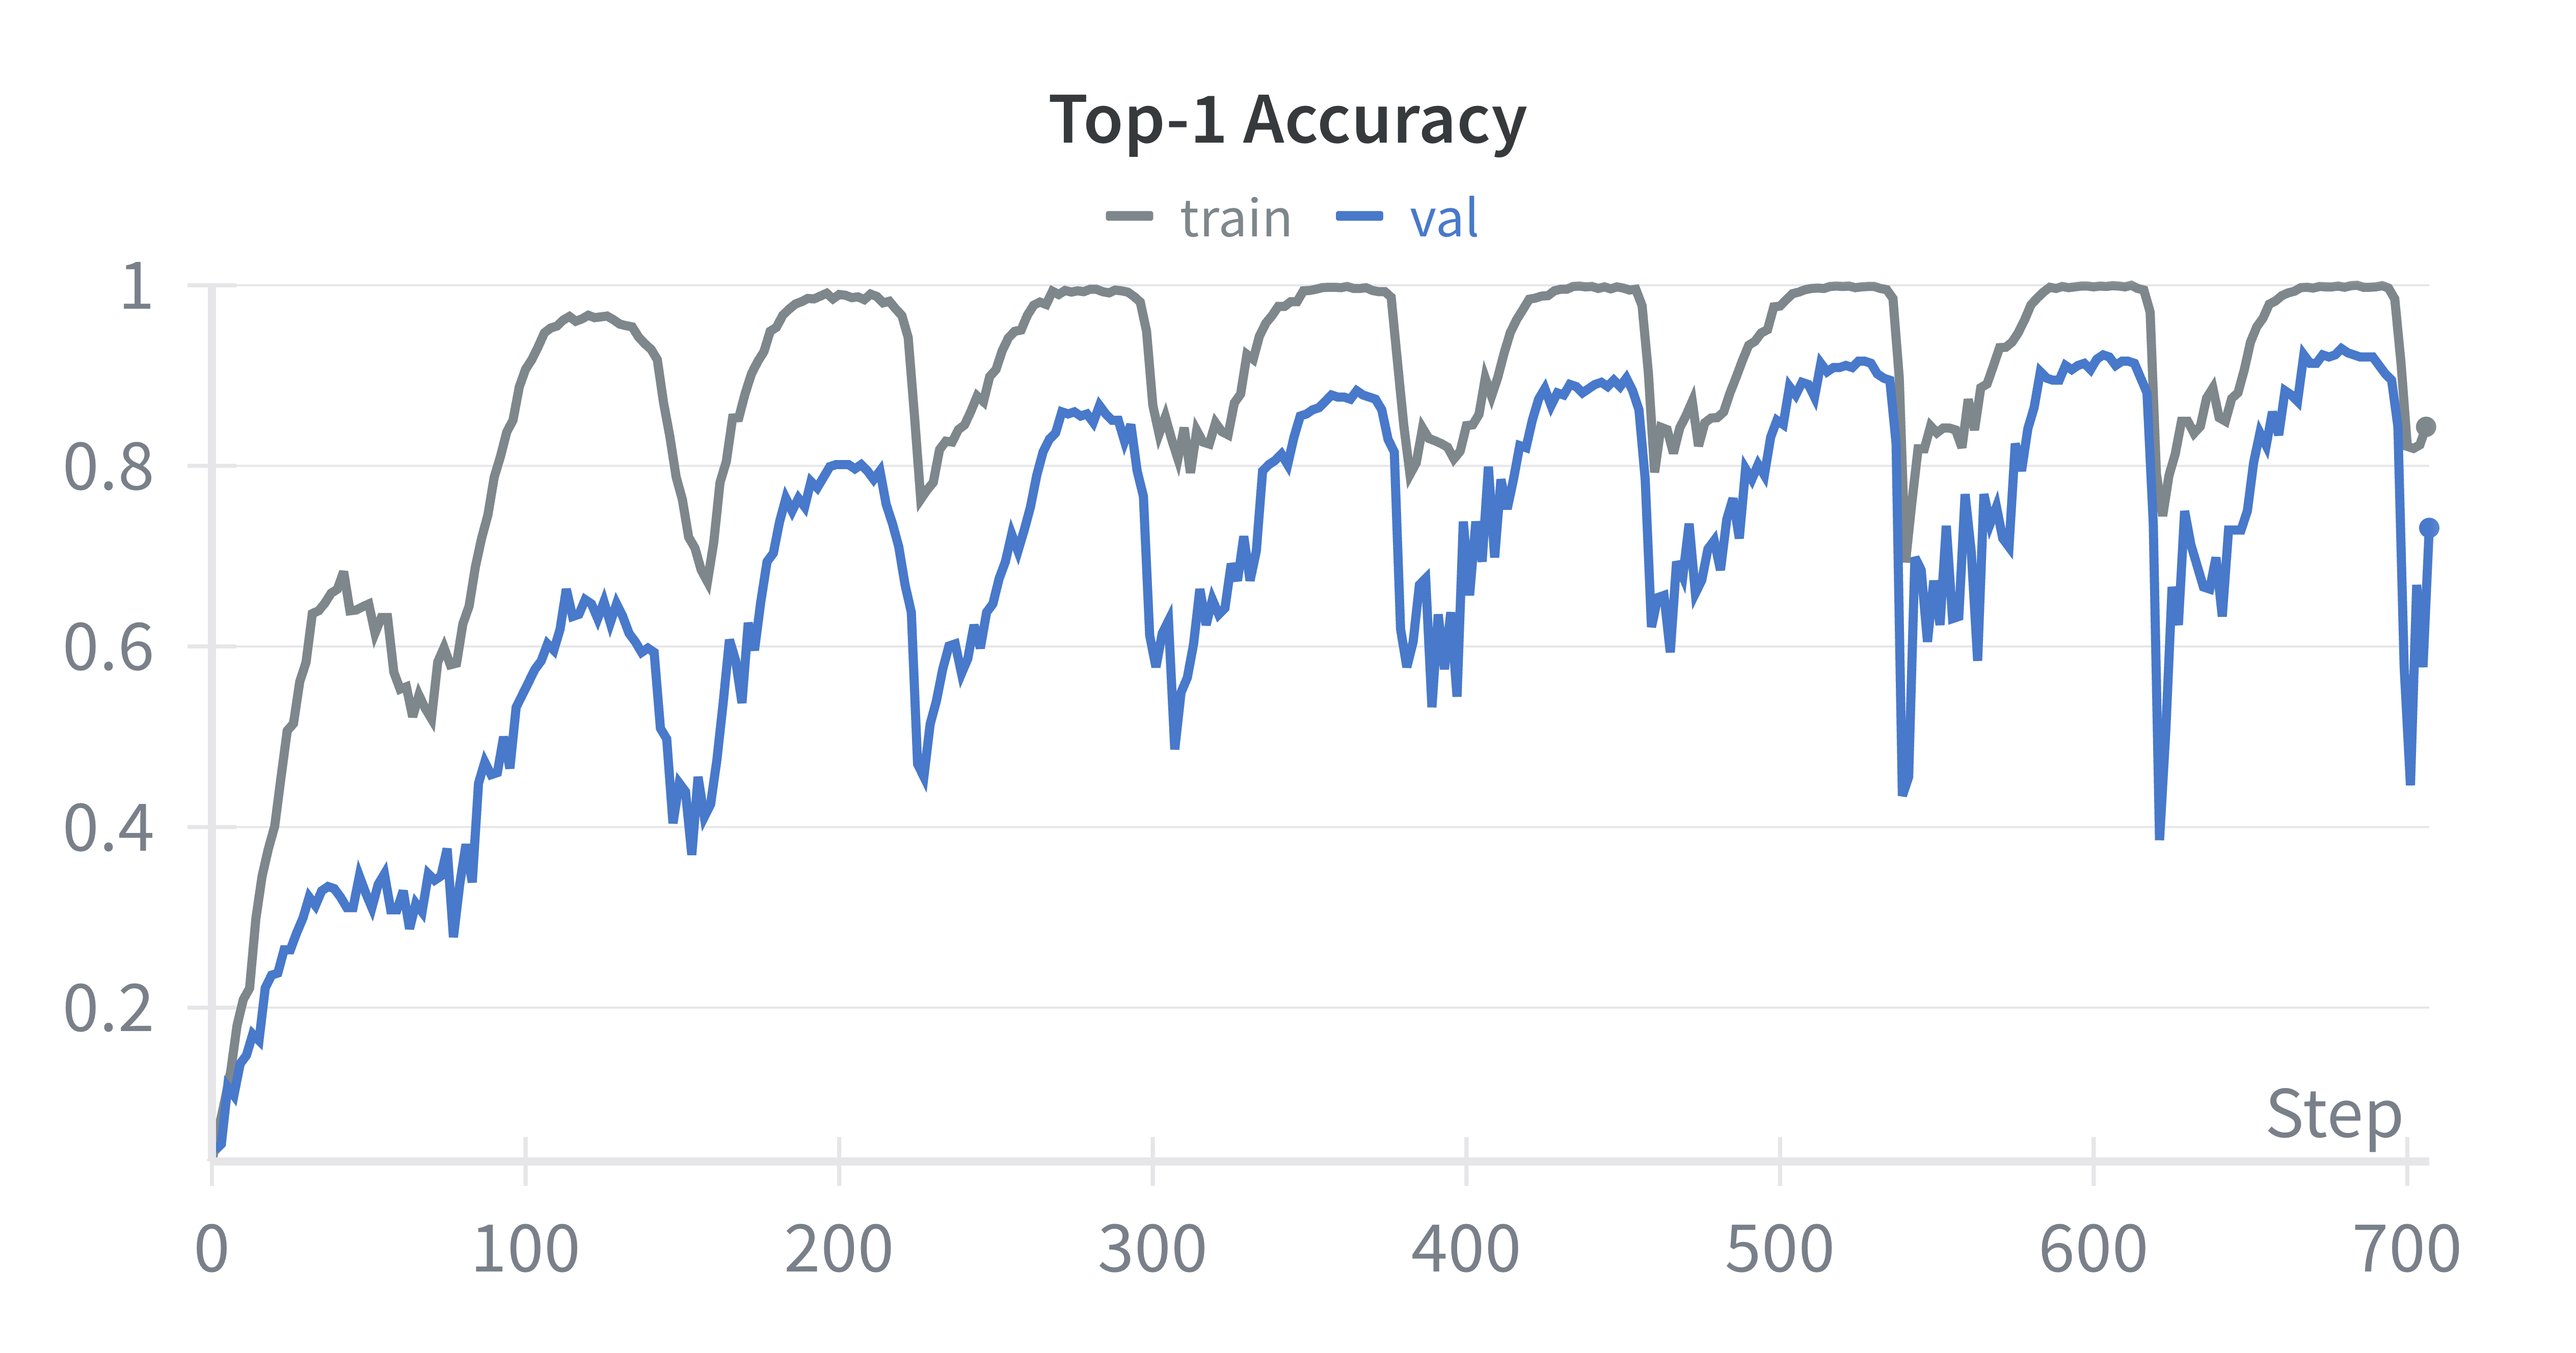
\includegraphics[width=\linewidth]{img_appendix/acc_all_moat_alphanum.png}
    \end{minipage}
    \caption{Alphanumeric keys}
\end{subfigure}
\vspace{0.5em}
\begin{subfigure}{\linewidth}
    \centering
    \begin{minipage}{0.49\linewidth}
        \centering
        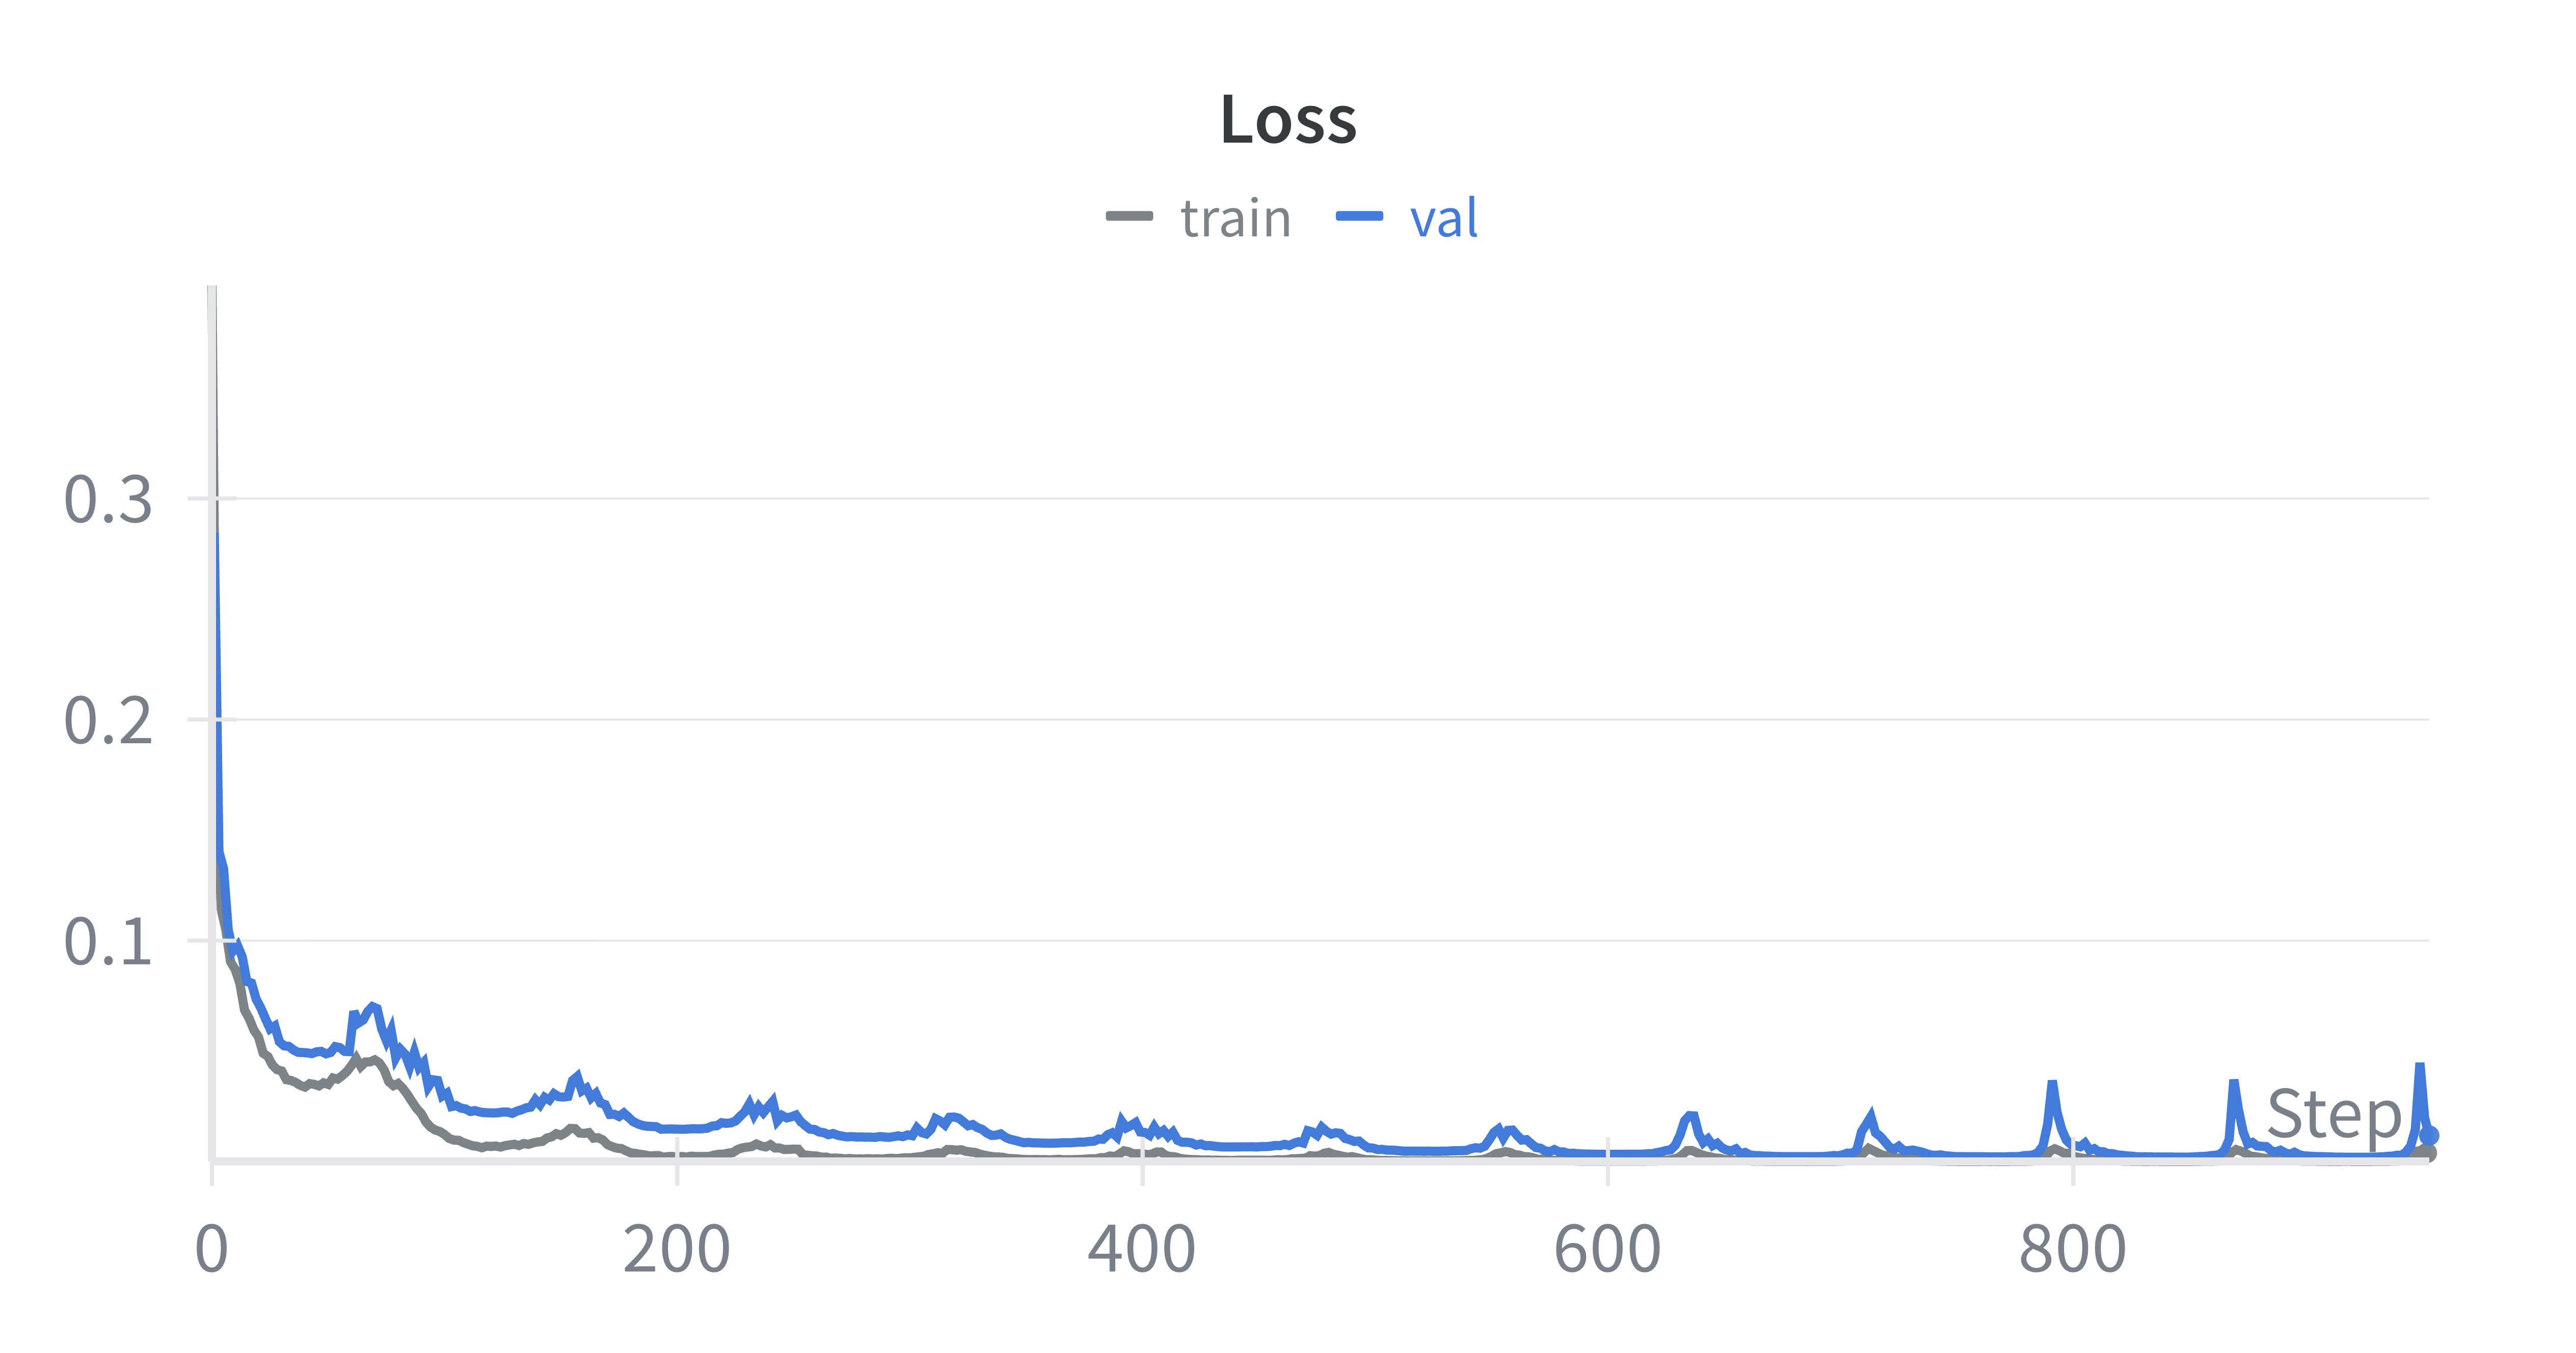
\includegraphics[width=\linewidth]{img_appendix/loss_all_moat_all.png}
    \end{minipage}
    \hfill
    \begin{minipage}{0.49\linewidth}
        \centering
        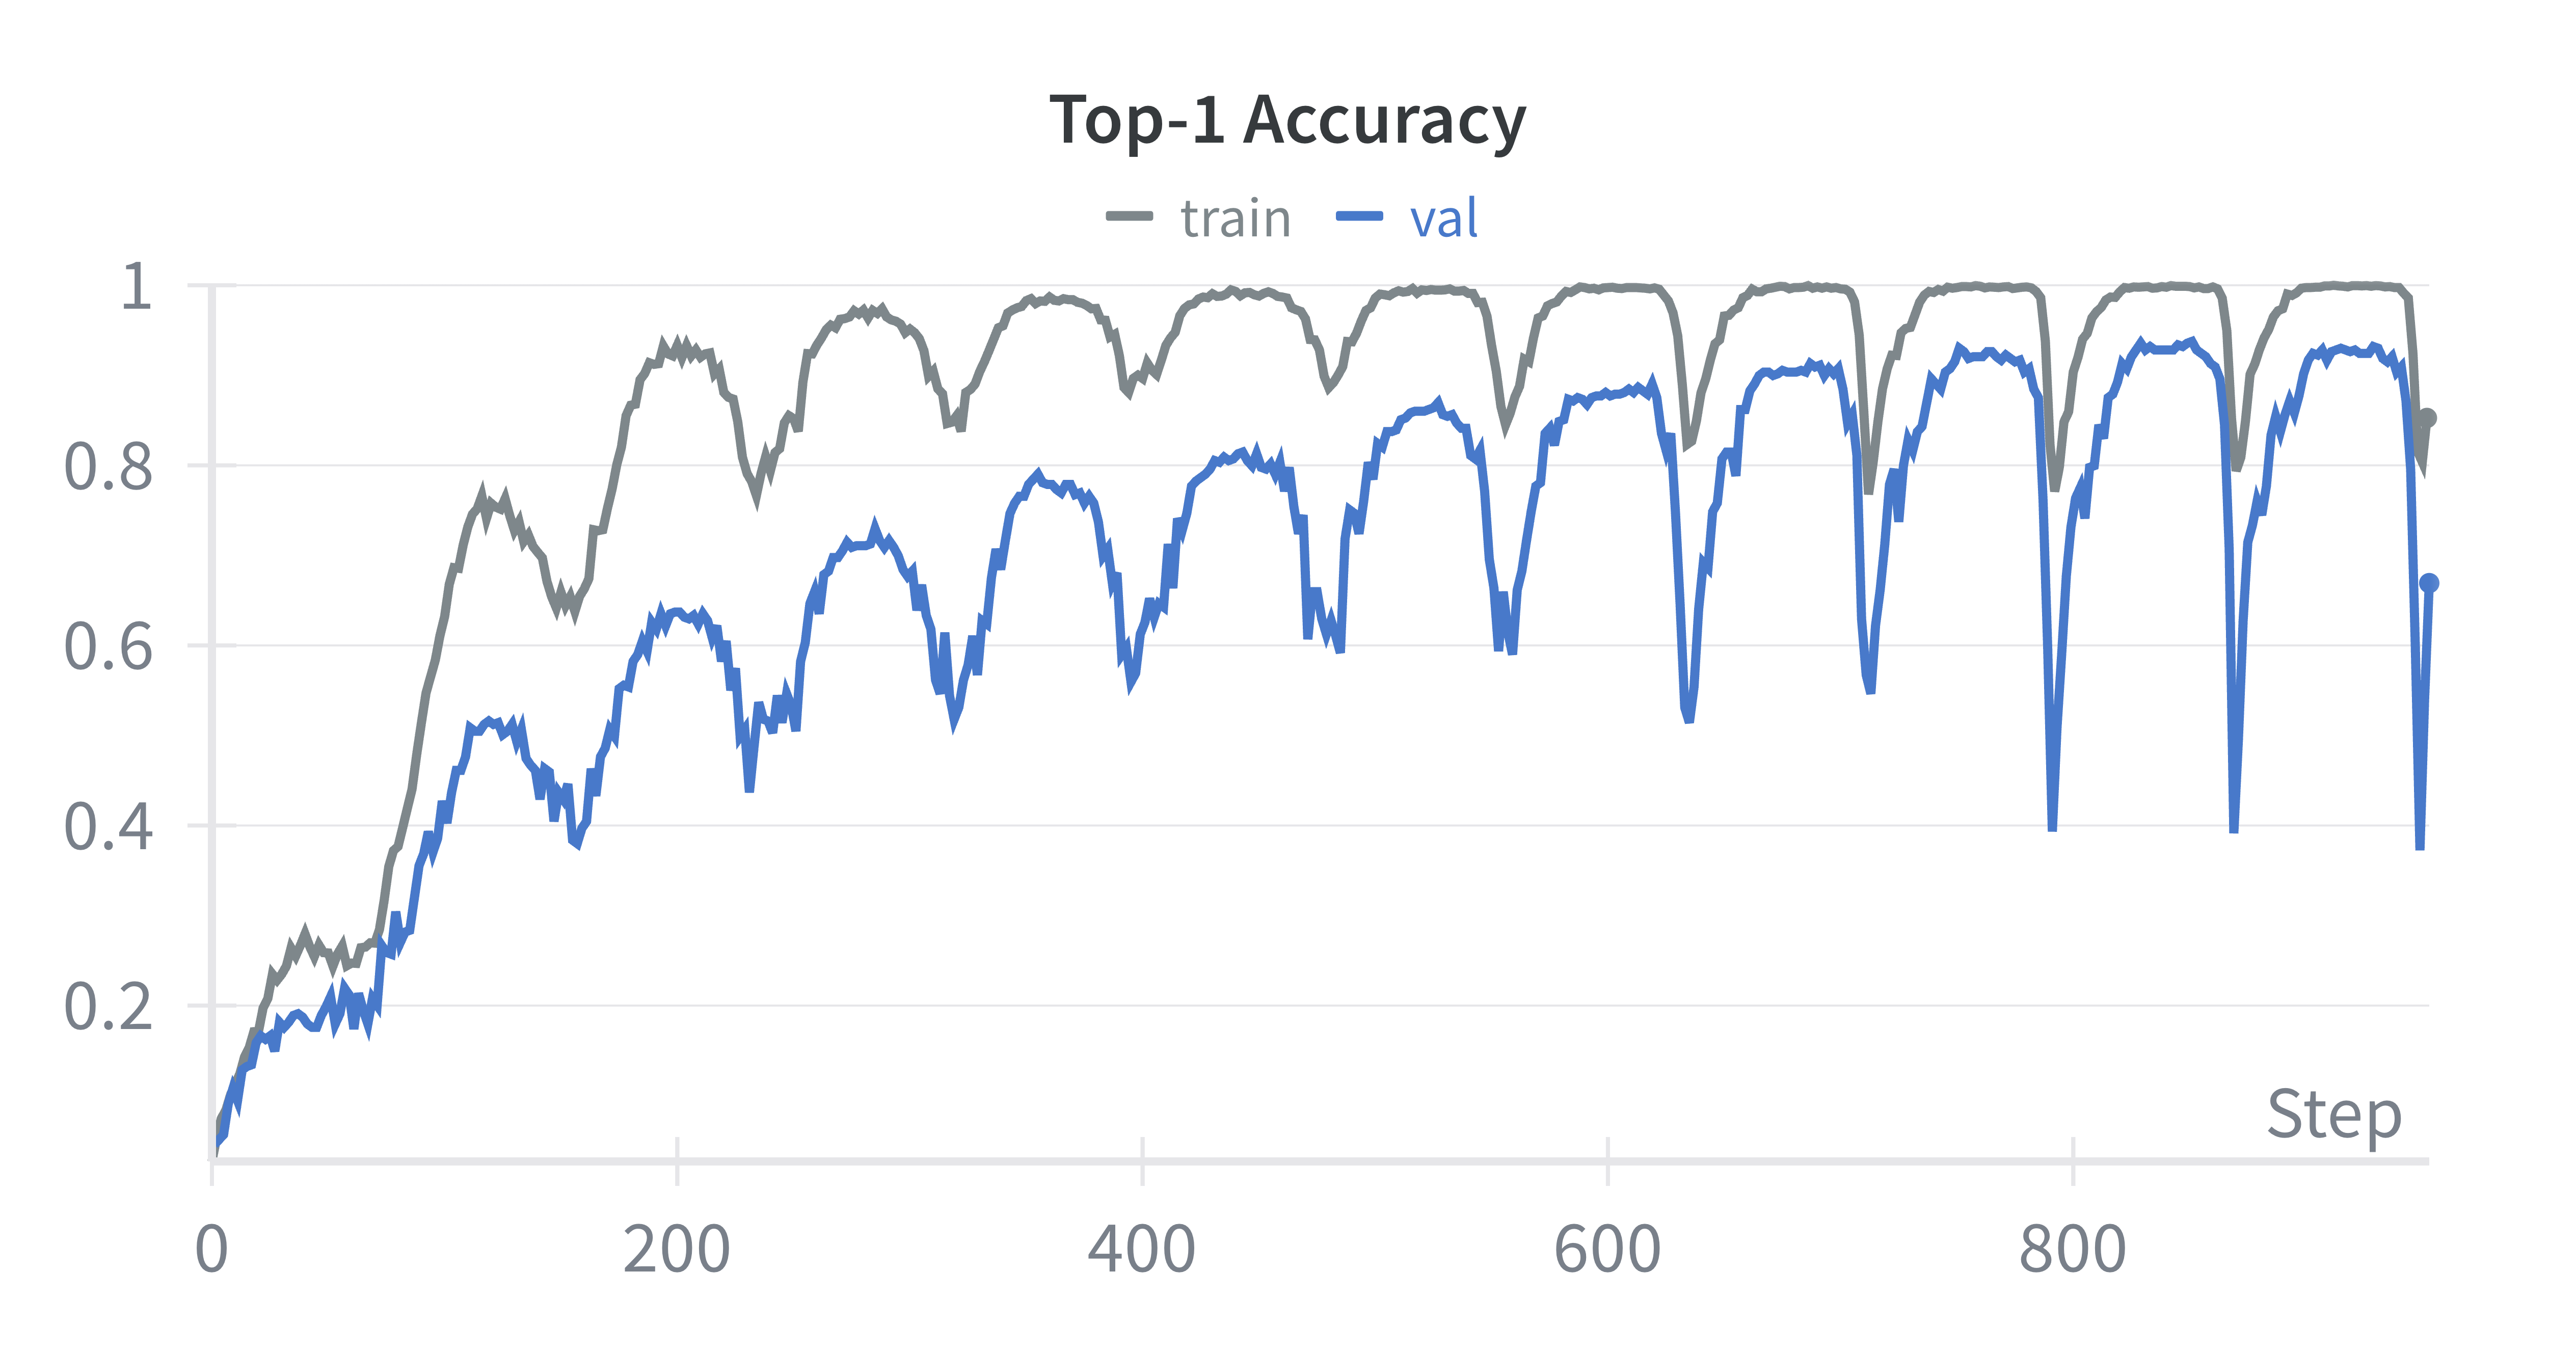
\includegraphics[width=\linewidth]{img_appendix/acc_all_moat_all.png}
    \end{minipage}
    \caption{All keys}
\end{subfigure}

\caption{Training histories of the best MOAT architectures on different sets of keys.}
\end{figure}

\begin{figure}[H]
\centering

\begin{subfigure}{\linewidth}
    \centering
    \begin{minipage}{0.49\linewidth}
        \centering
        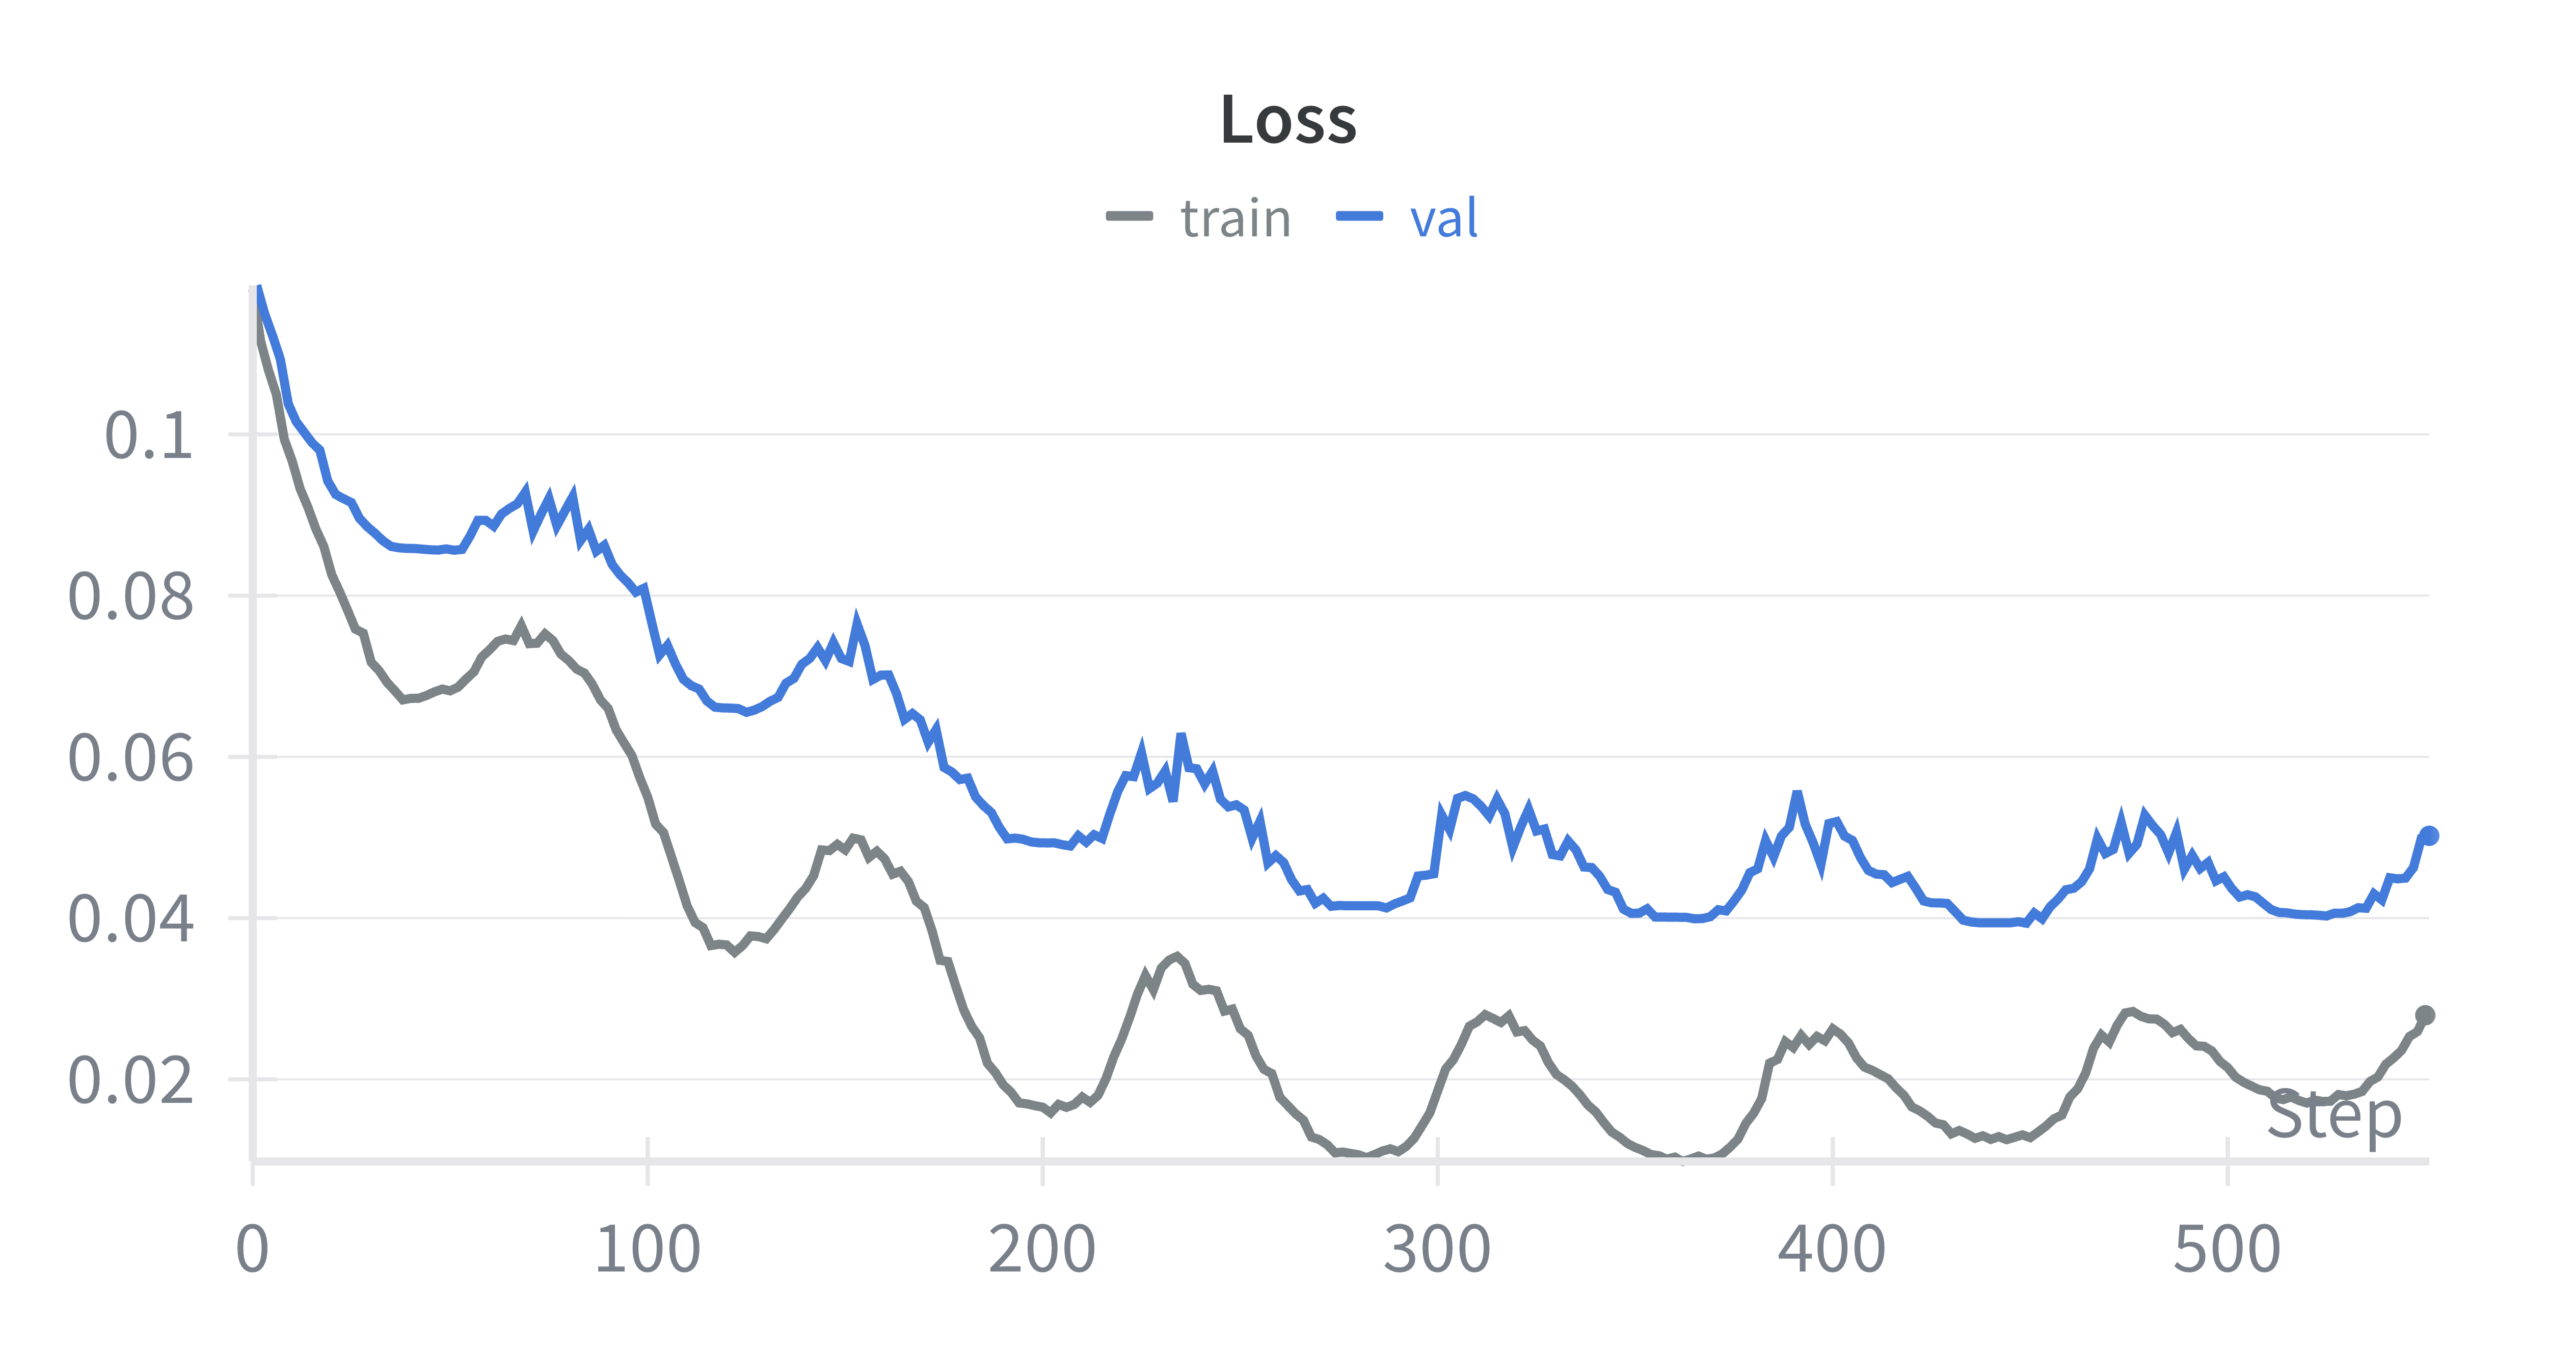
\includegraphics[width=\linewidth]{img_appendix/loss_all_swin_alphanum.png}
    \end{minipage}
    \hfill
    \begin{minipage}{0.49\linewidth}
        \centering
        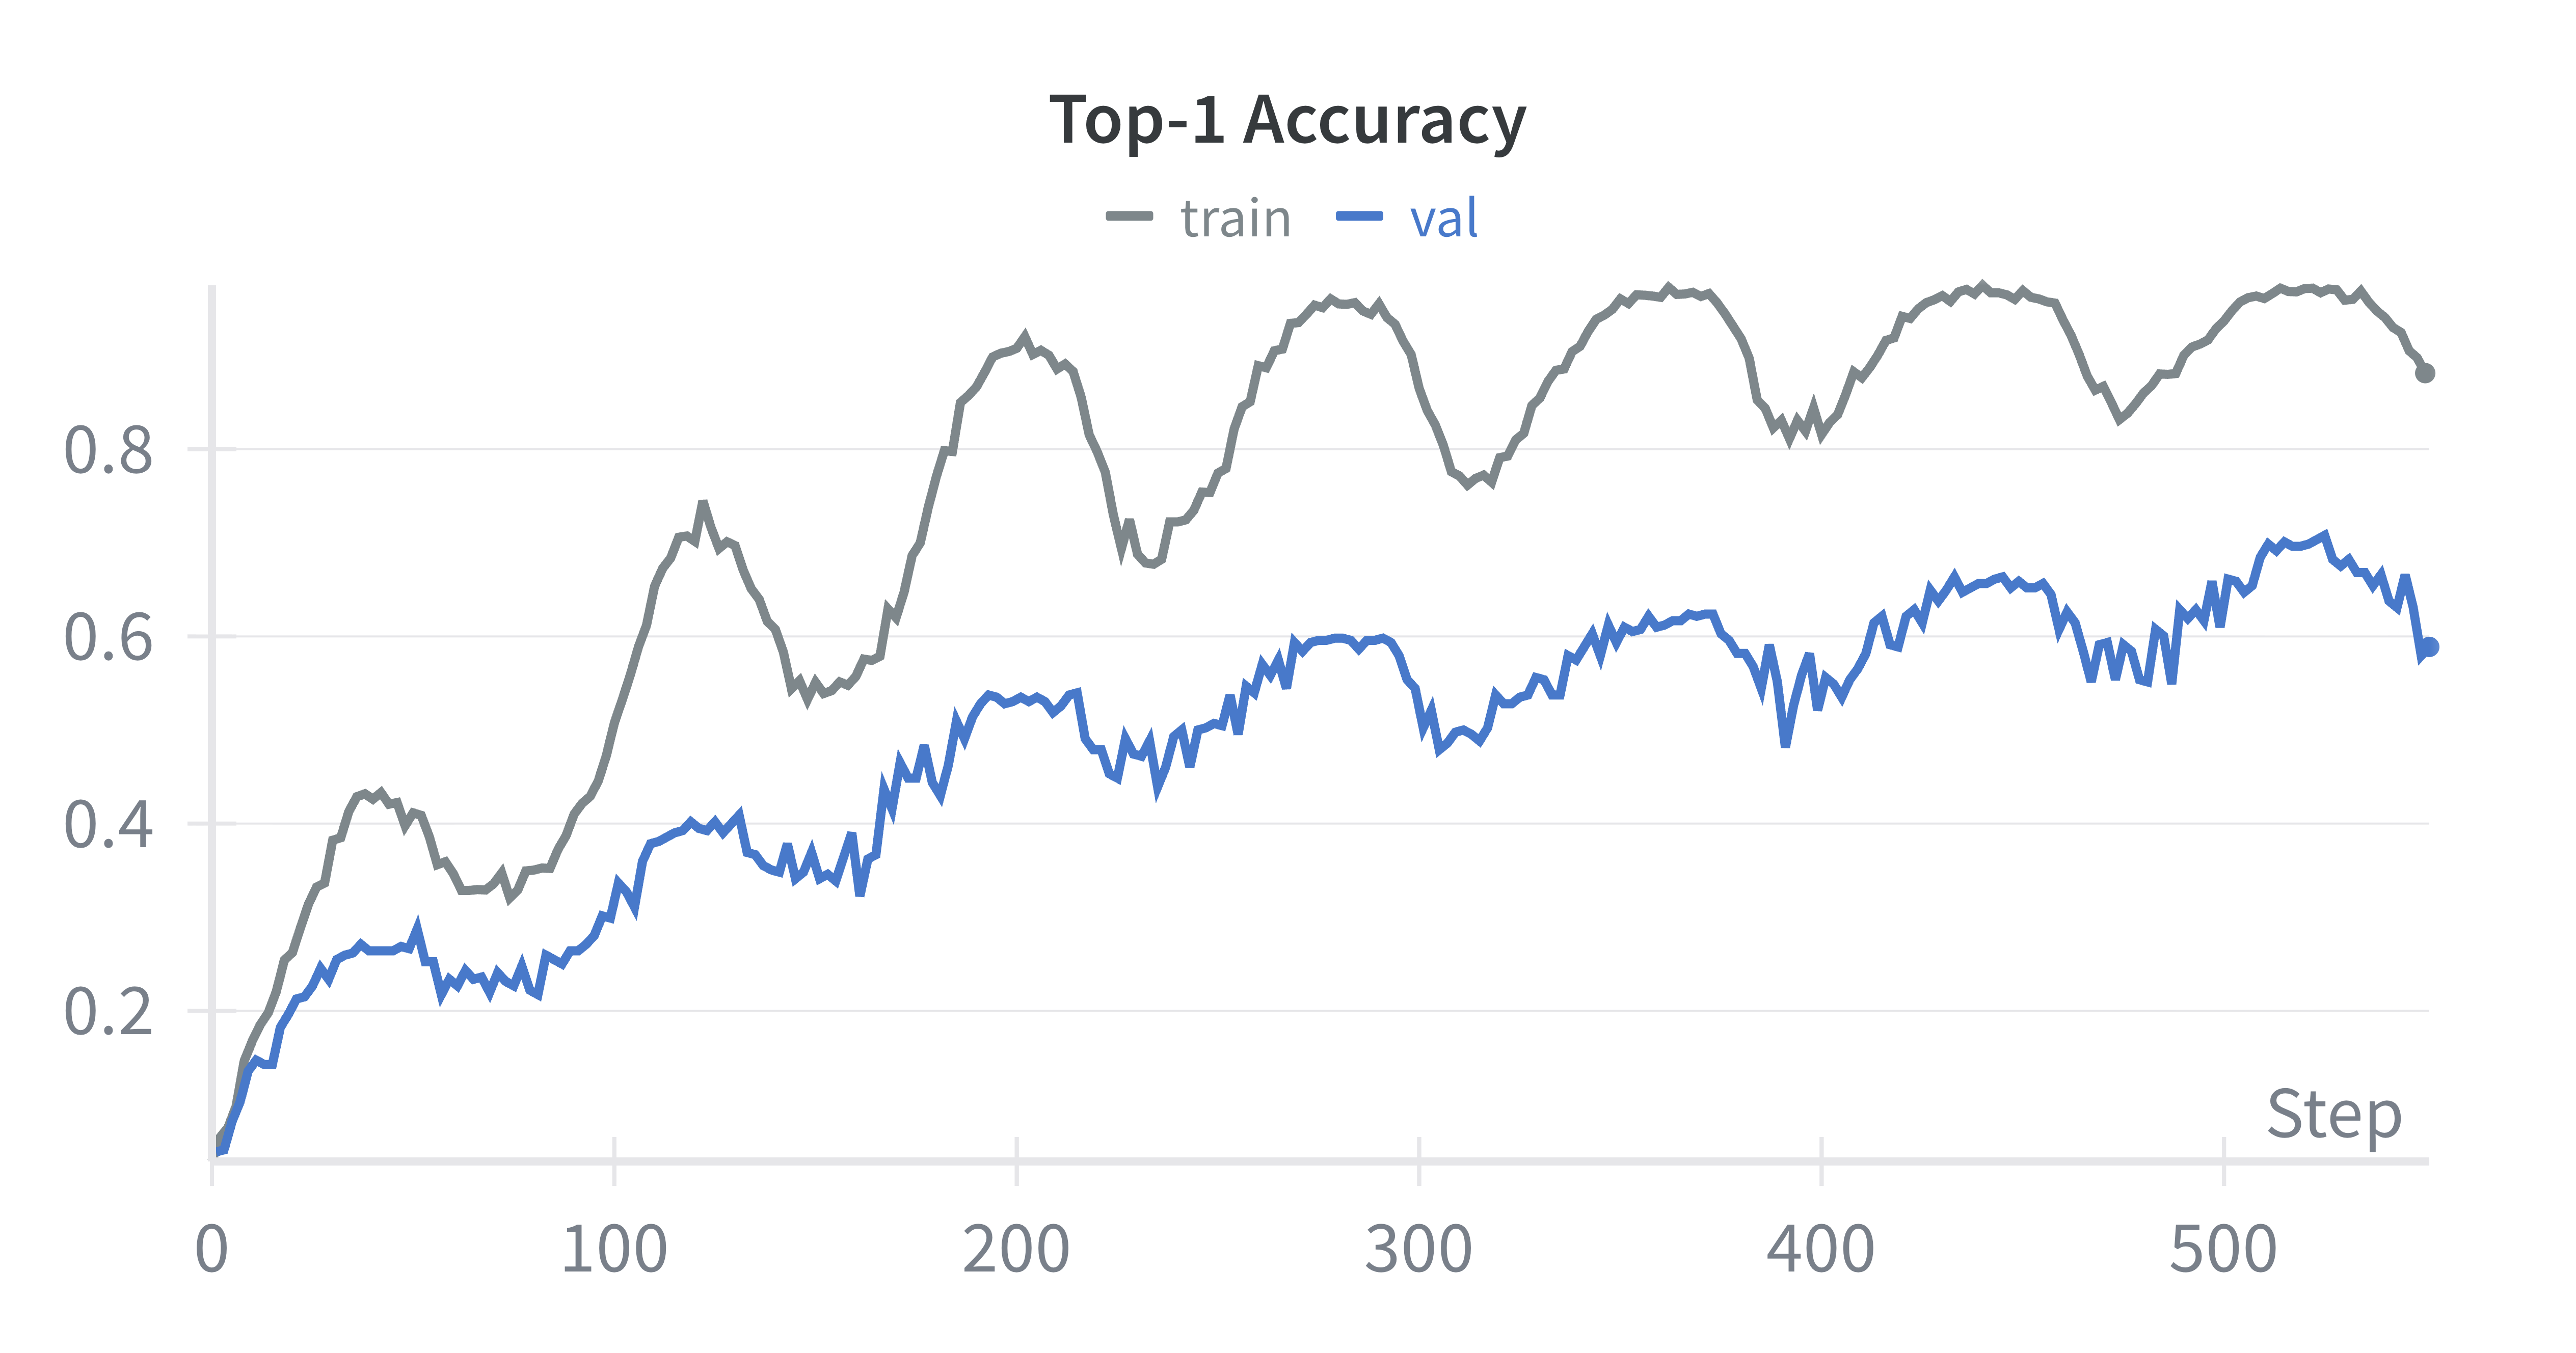
\includegraphics[width=\linewidth]{img_appendix/acc_all_swin_alphanum.png}
    \end{minipage}
    \caption{Alphanumeric keys}
\end{subfigure}
\vspace{0.5em}
\begin{subfigure}{\linewidth}
    \centering
    \begin{minipage}{0.49\linewidth}
        \centering
        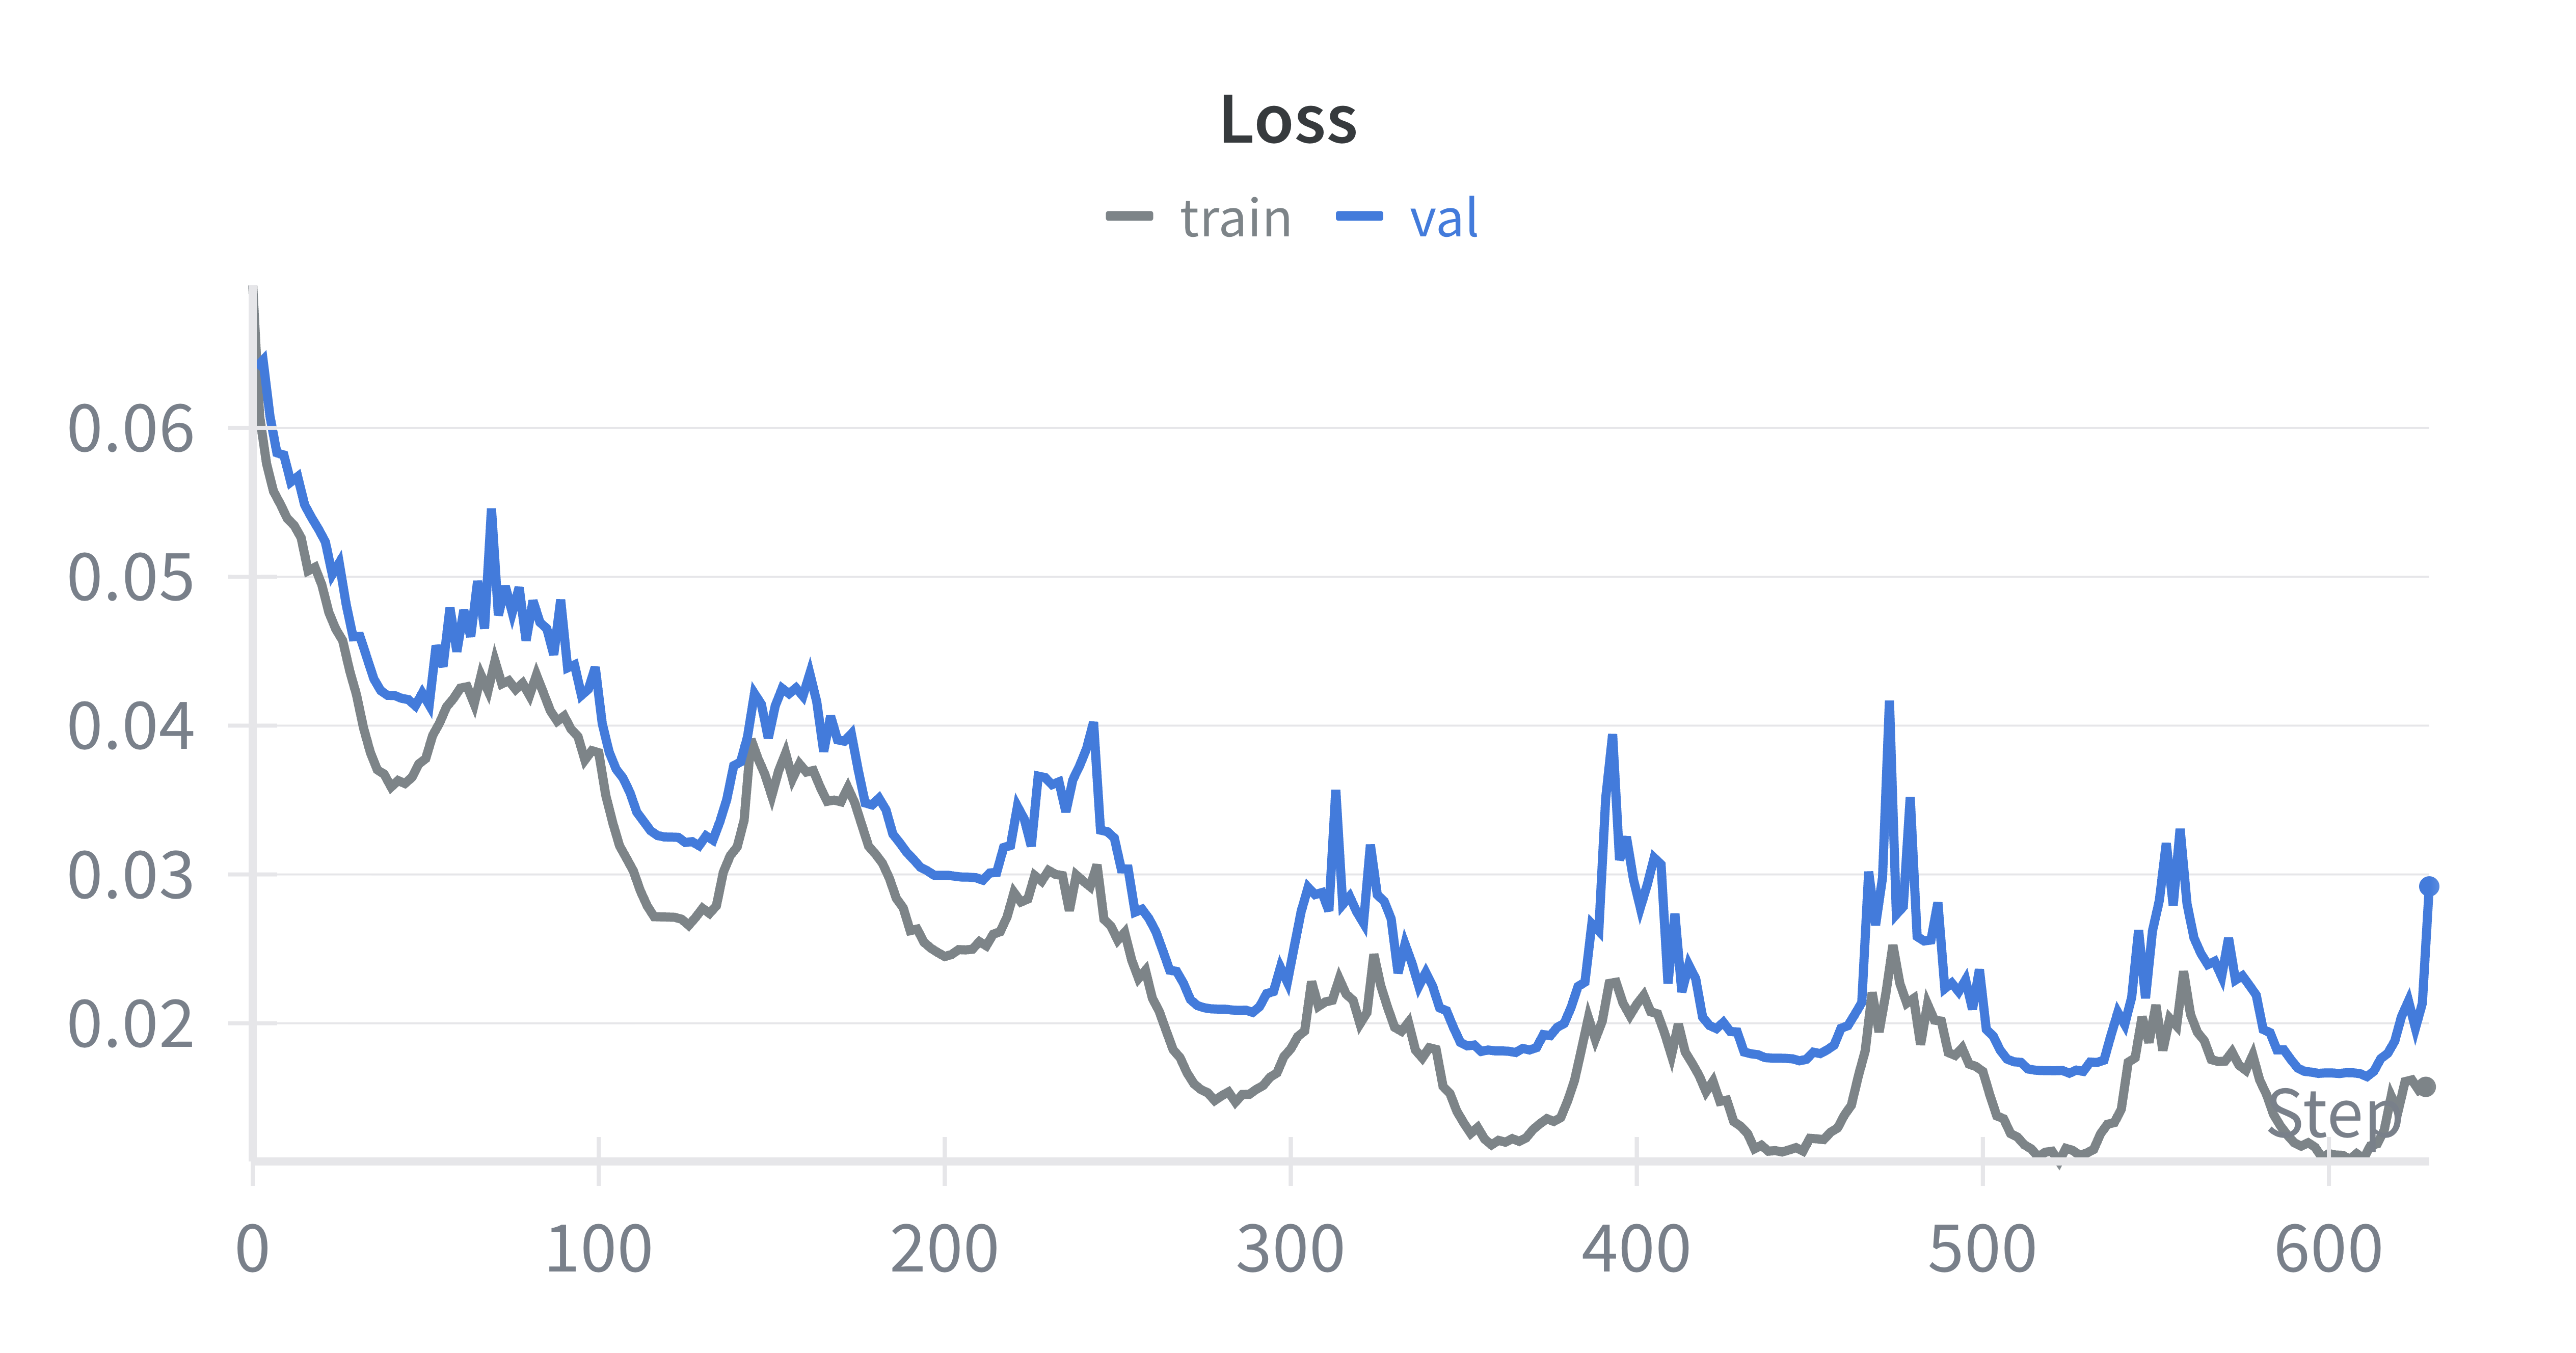
\includegraphics[width=\linewidth]{img_appendix/loss_all_swin_all.png}
    \end{minipage}
    \hfill
    \begin{minipage}{0.49\linewidth}
        \centering
        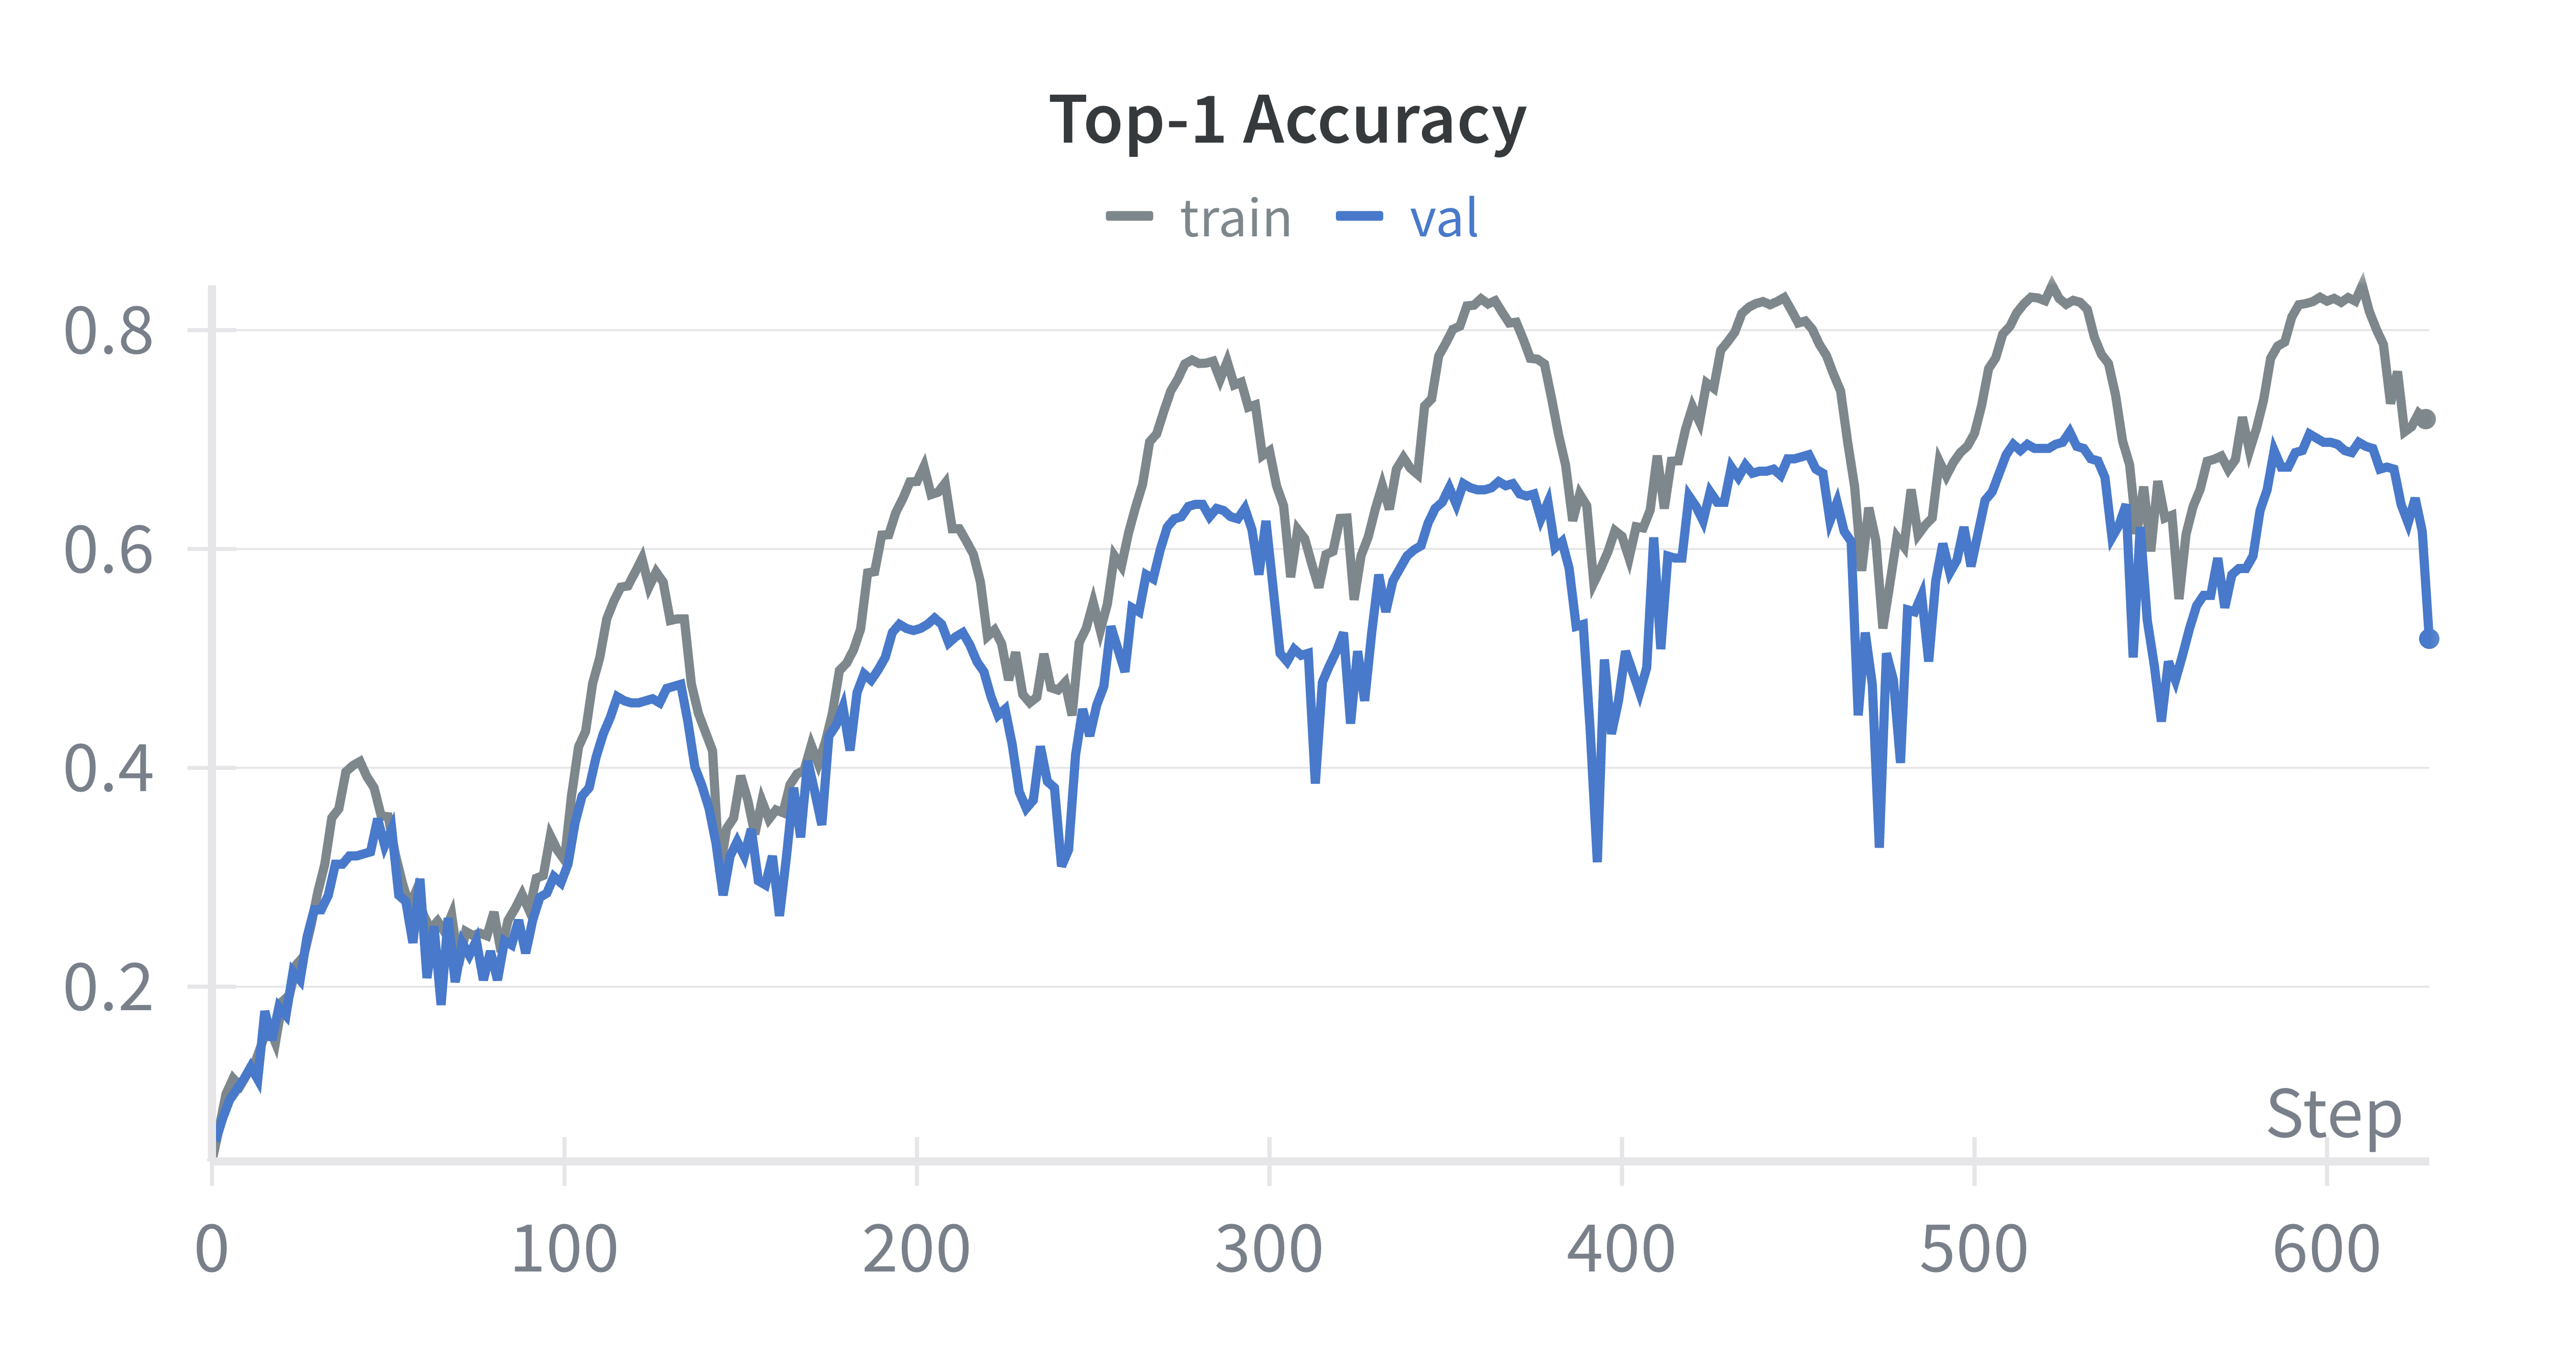
\includegraphics[width=\linewidth]{img_appendix/acc_all_swin_all.png}
    \end{minipage}
    \caption{All keys}
\end{subfigure}

\caption{Training histories of the best Swin Transformer architectures on different sets of keys.}
\end{figure}

\begin{figure}[H]
  \centering
    \begin{minipage}{0.49\linewidth}
      \centering
      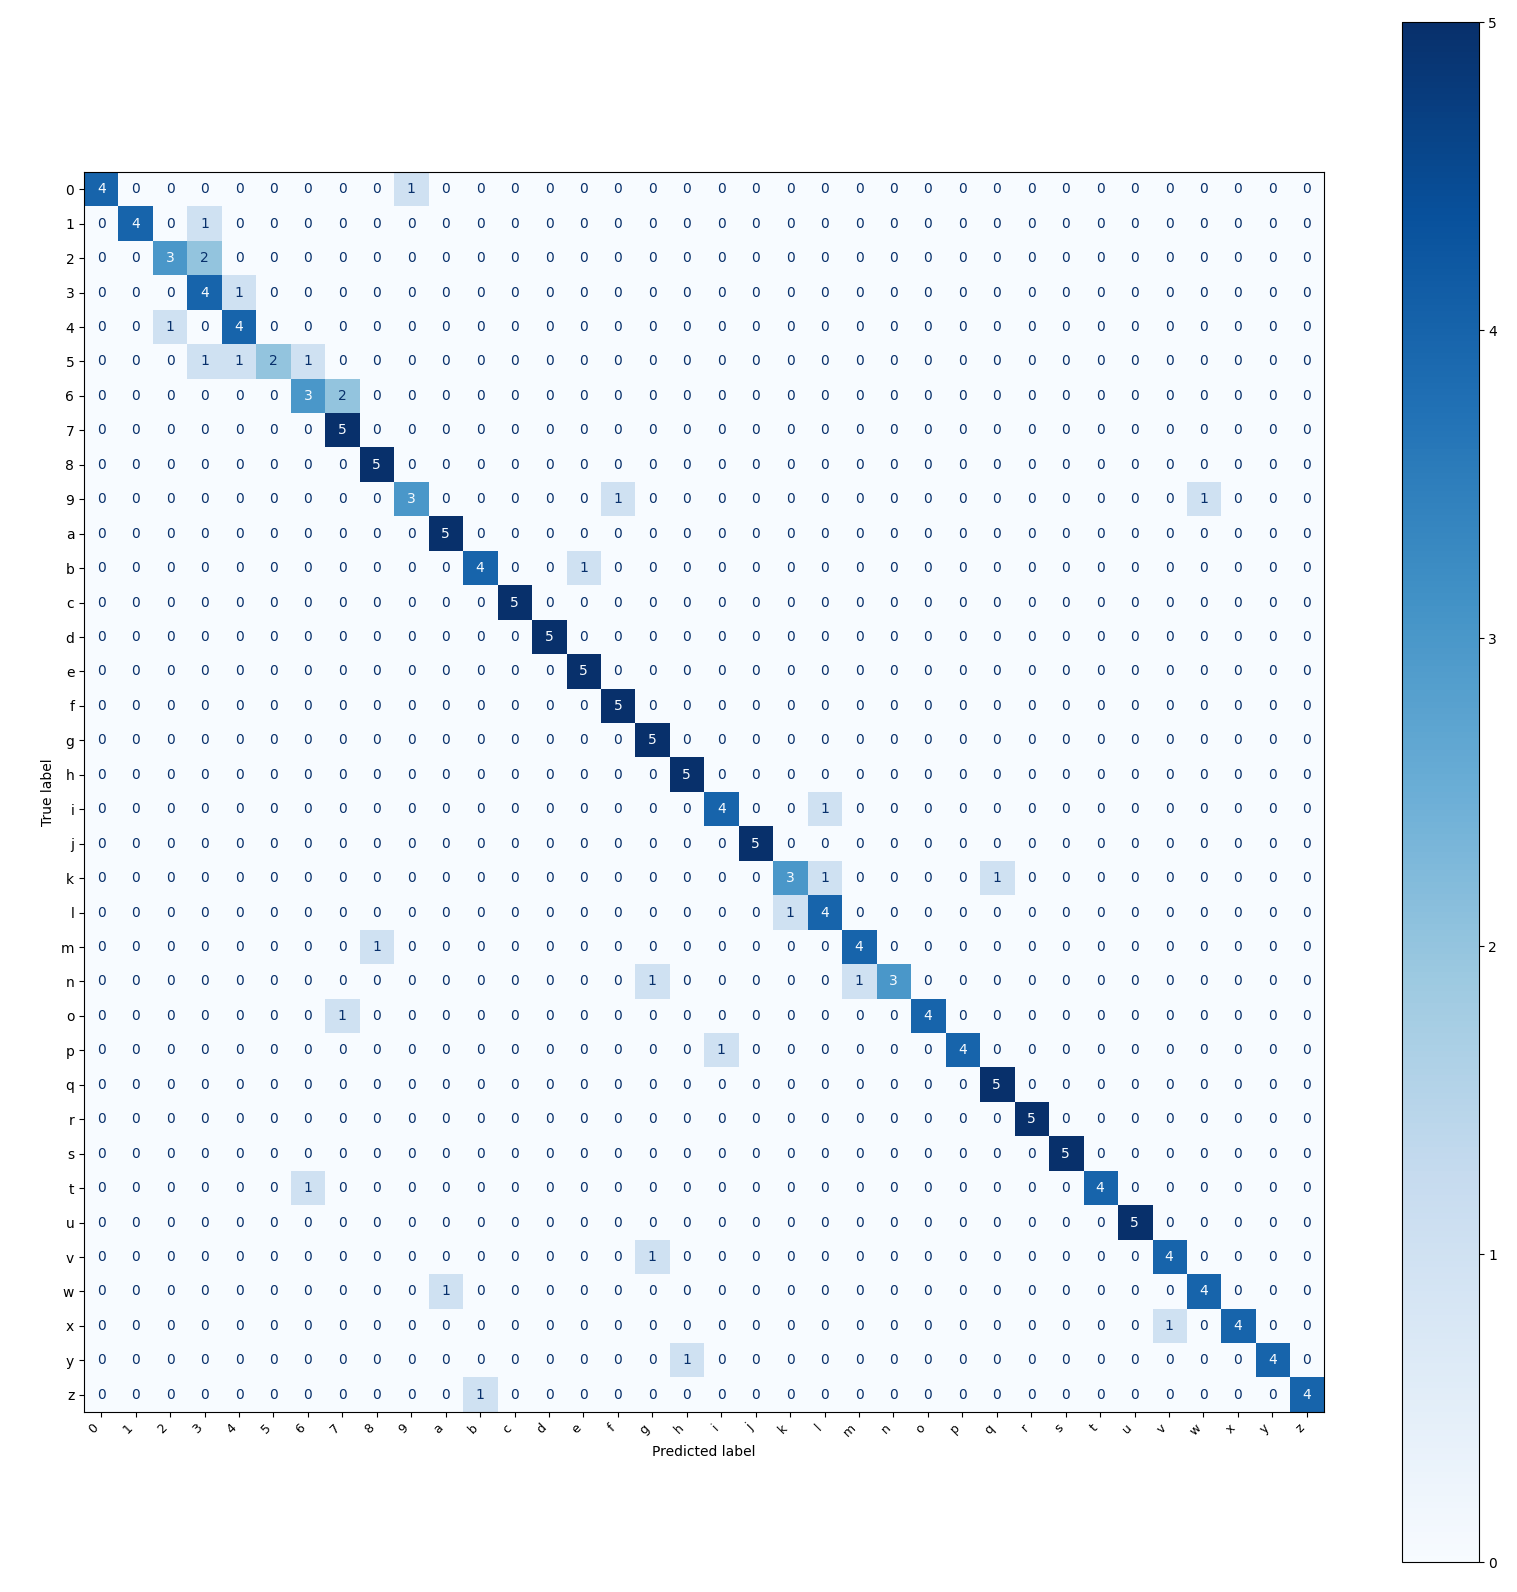
\includegraphics[width=\linewidth]{img_appendix/cm_all_alphanum_mka.png}
      \subcaption{MKA dataset}
  \end{minipage}
  \begin{minipage}{0.49\linewidth}
      \centering
      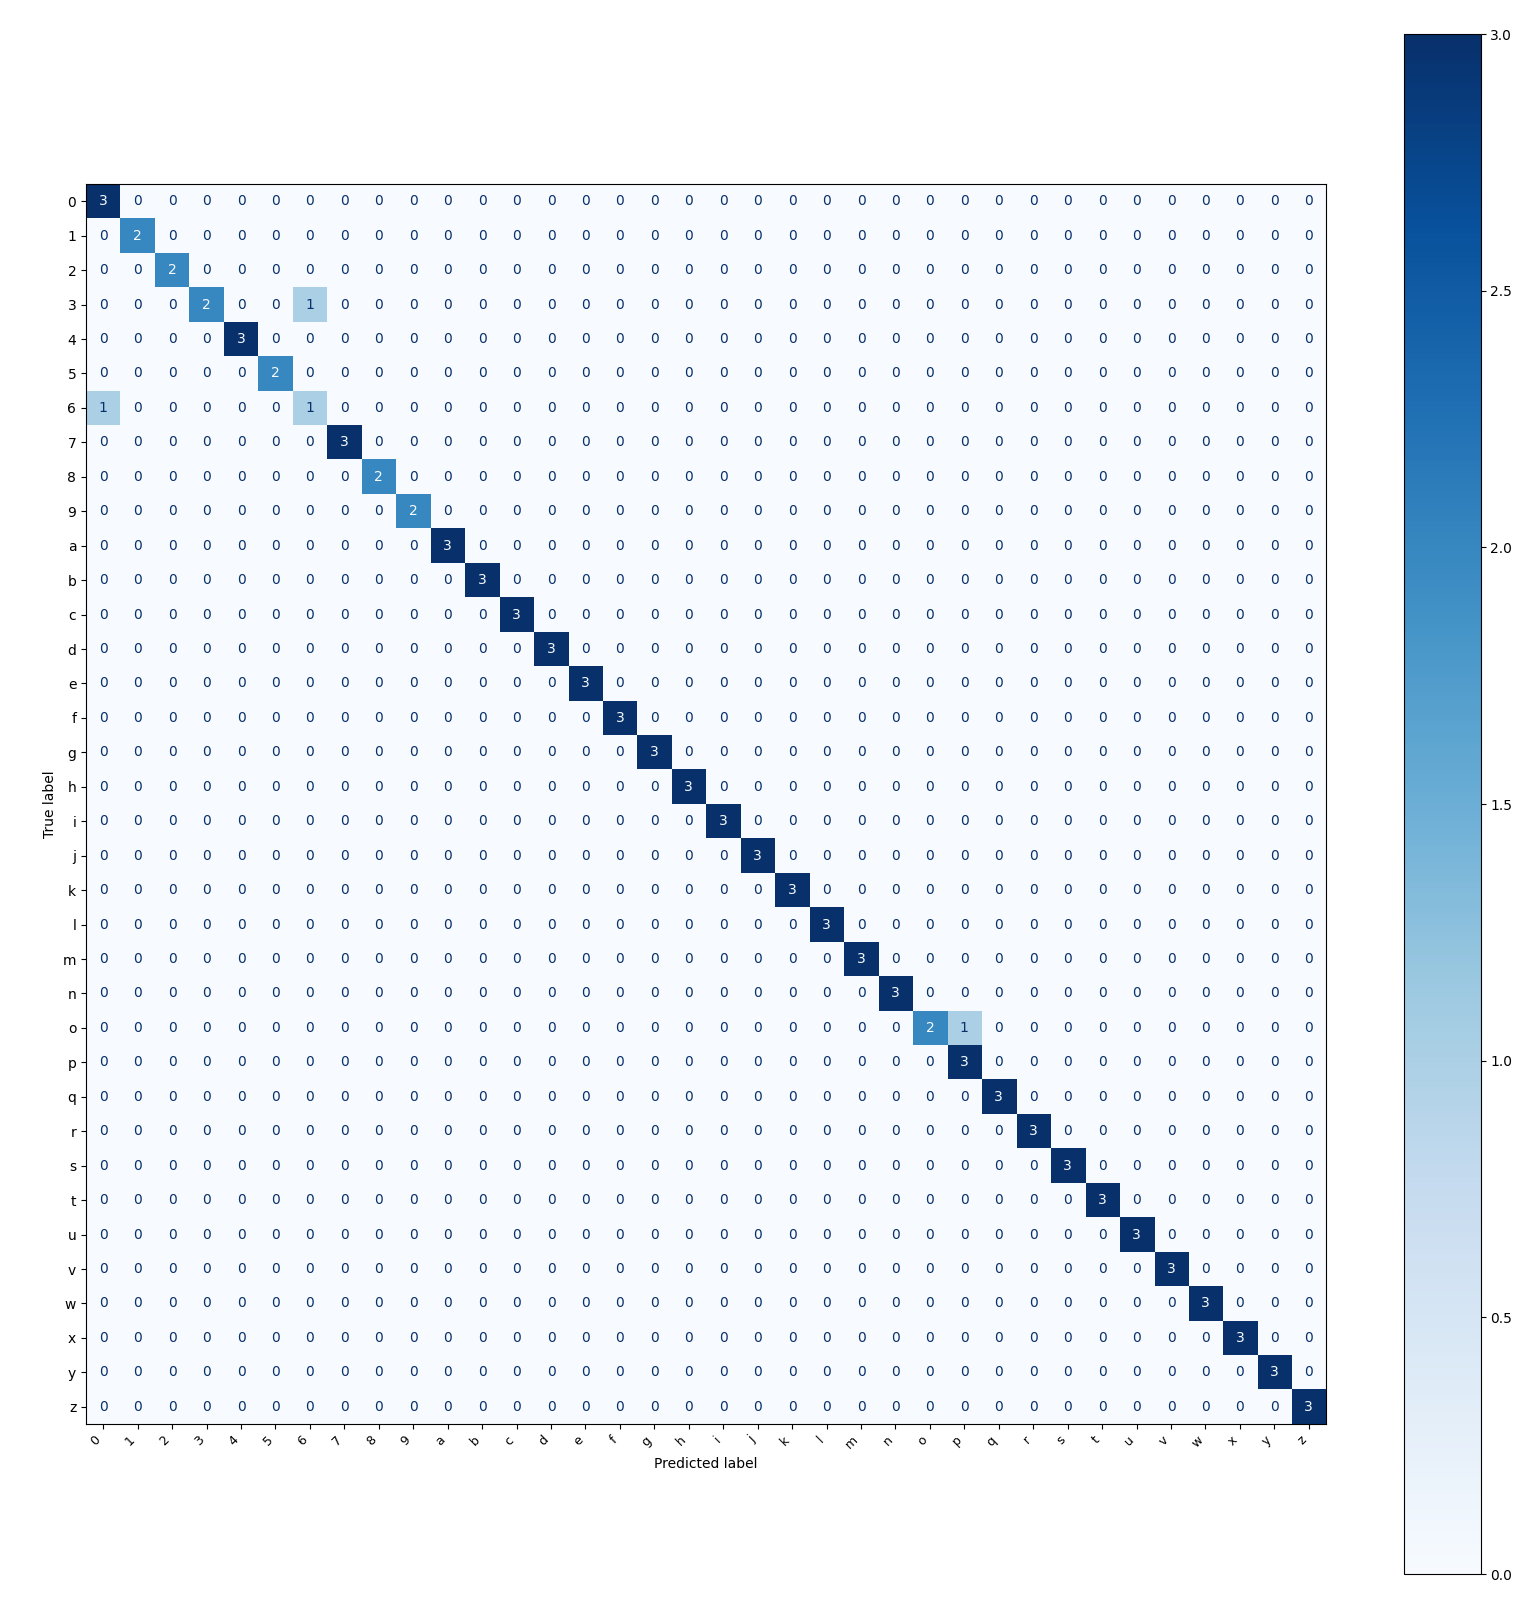
\includegraphics[width=\linewidth]{img_appendix/cm_all_alphanum_n.png}
      \subcaption{Noiseless dataset}
  \end{minipage}
  \hfill
  \begin{minipage}{0.49\linewidth}
      \centering
      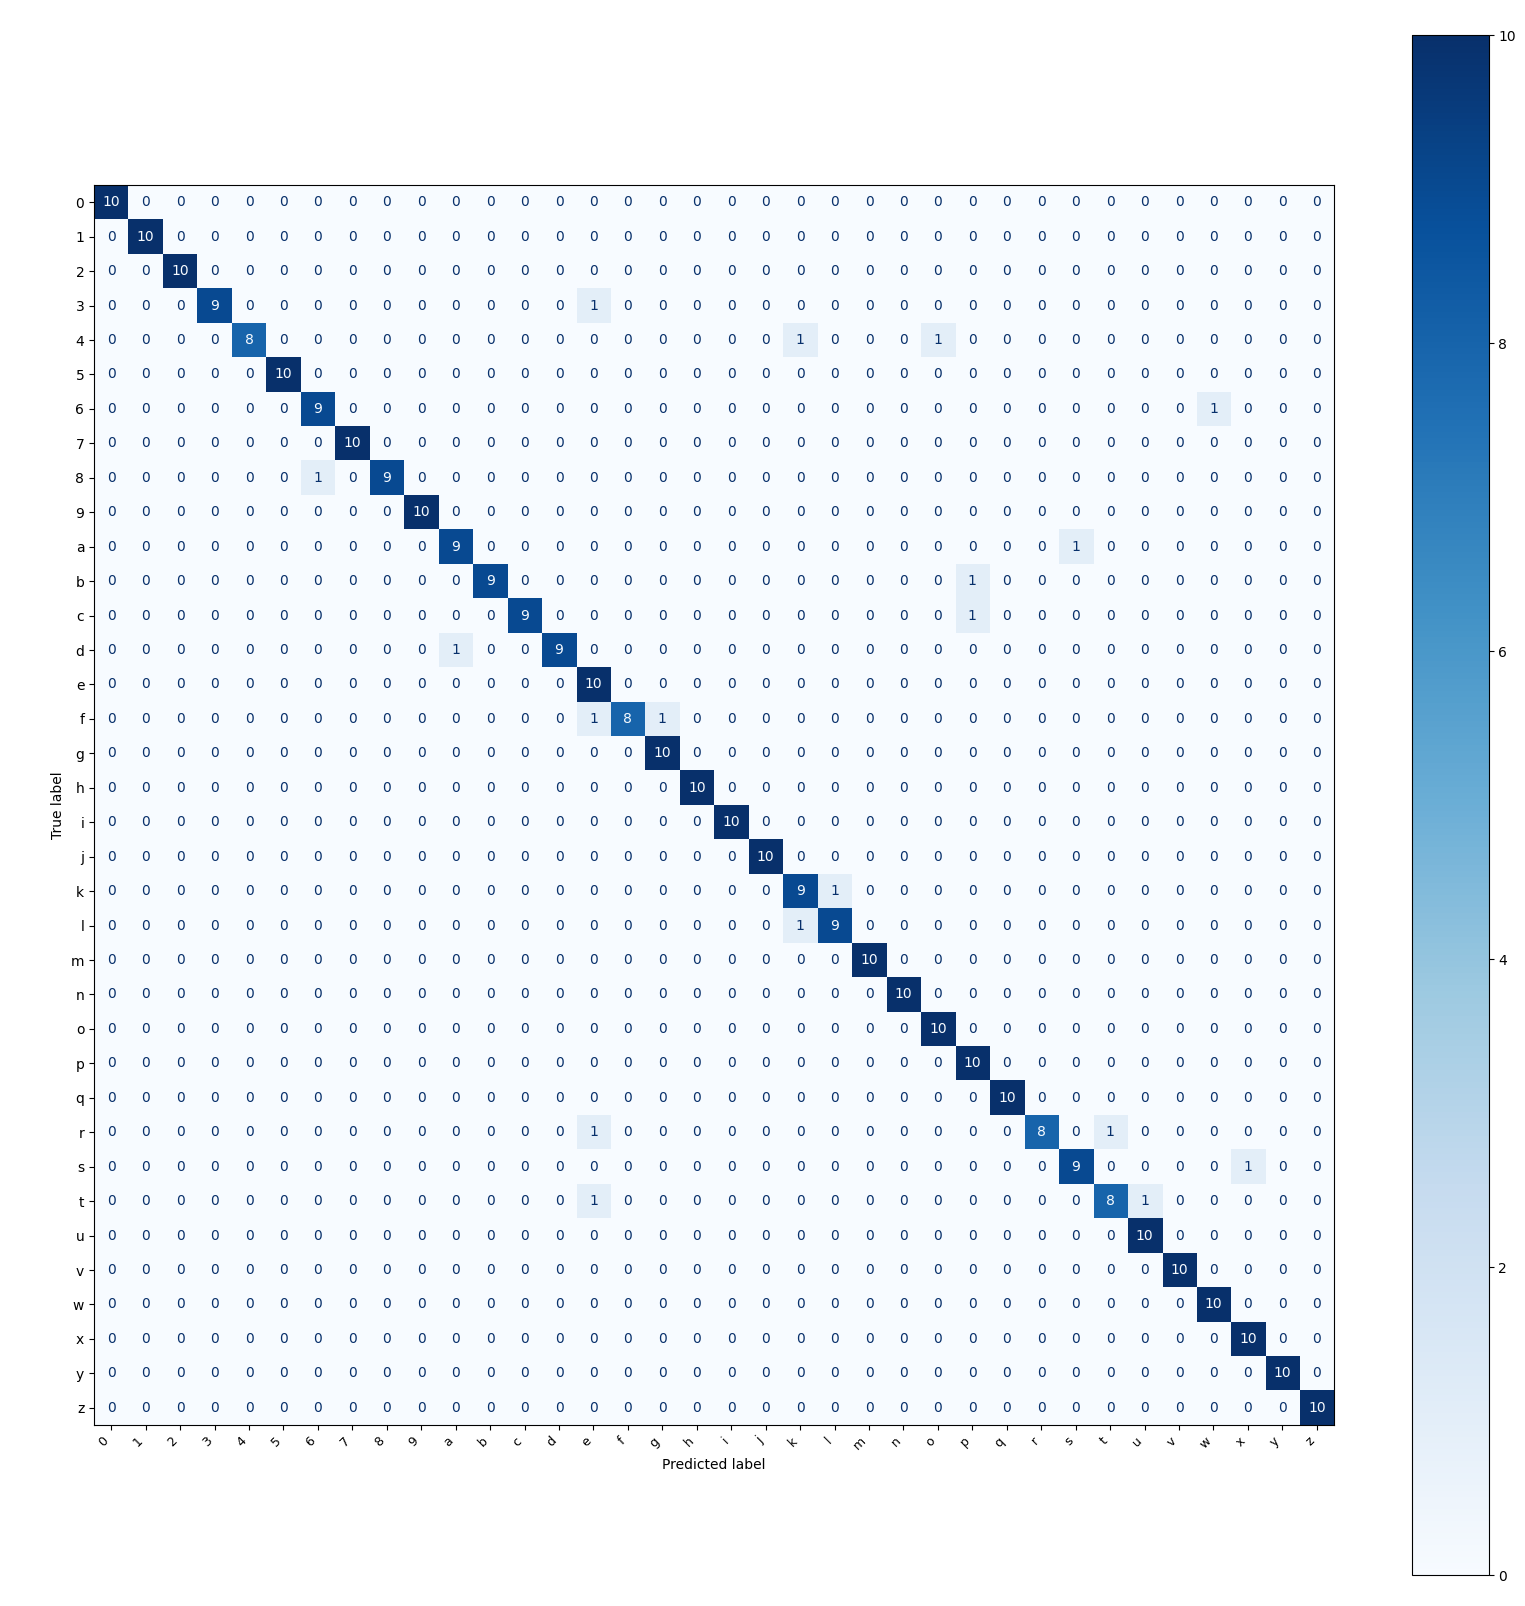
\includegraphics[width=\linewidth]{img_appendix/cm_all_alphanum_p.png}
      \subcaption{Practical dataset}
  \end{minipage}
  \caption{Confusion matrices of the best CoAtNet model using alphanumeric keys evaluated on different datasets.}
\end{figure}

\begin{figure}[H]
  \centering
    \begin{minipage}{0.49\linewidth}
      \centering
      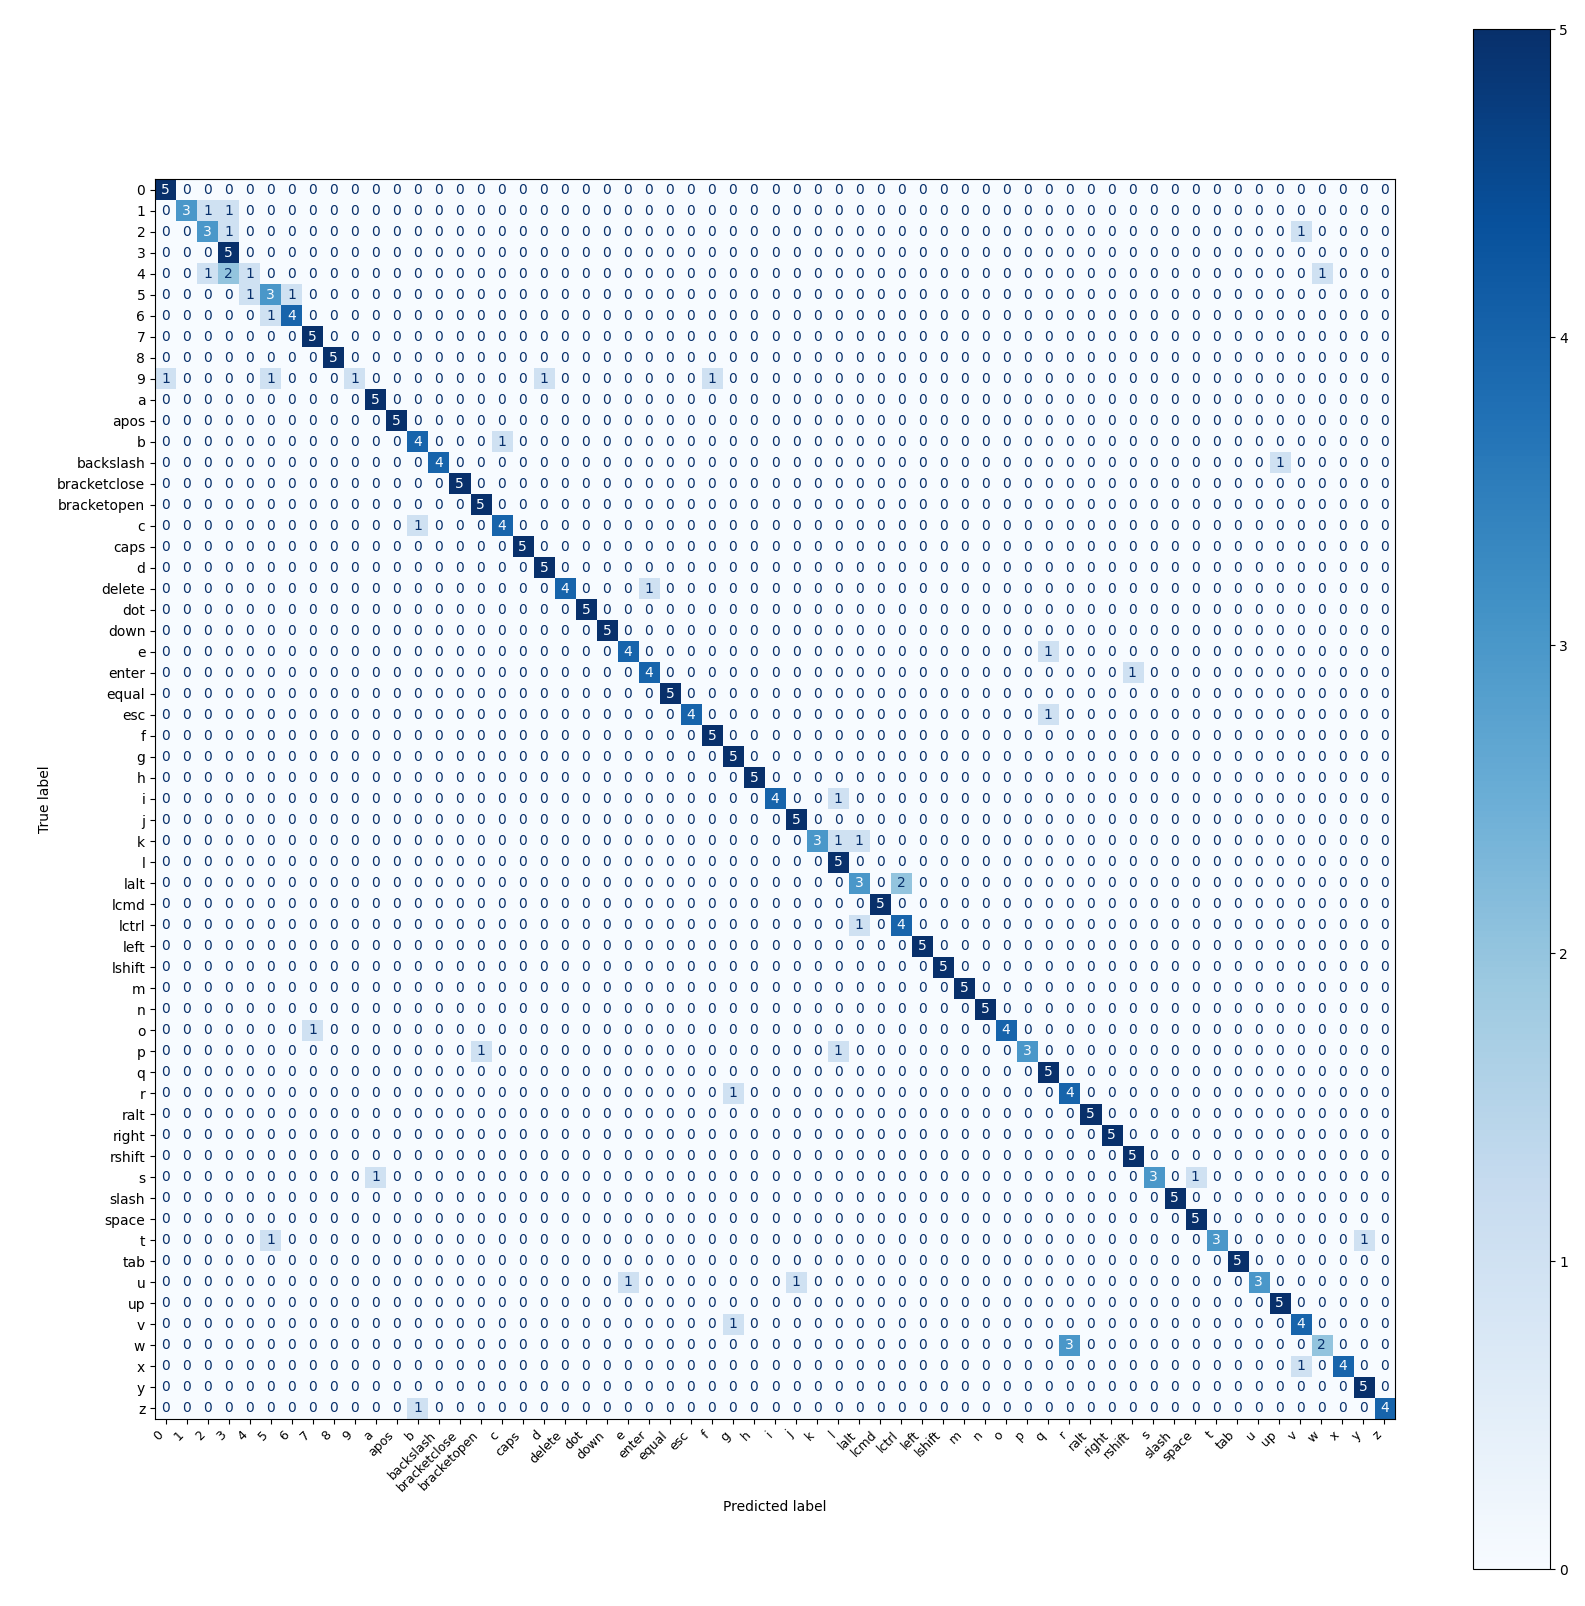
\includegraphics[width=\linewidth]{img_appendix/cm_all_all_mka.png}
      \subcaption{MKA dataset}
  \end{minipage}
  \begin{minipage}{0.49\linewidth}
      \centering
      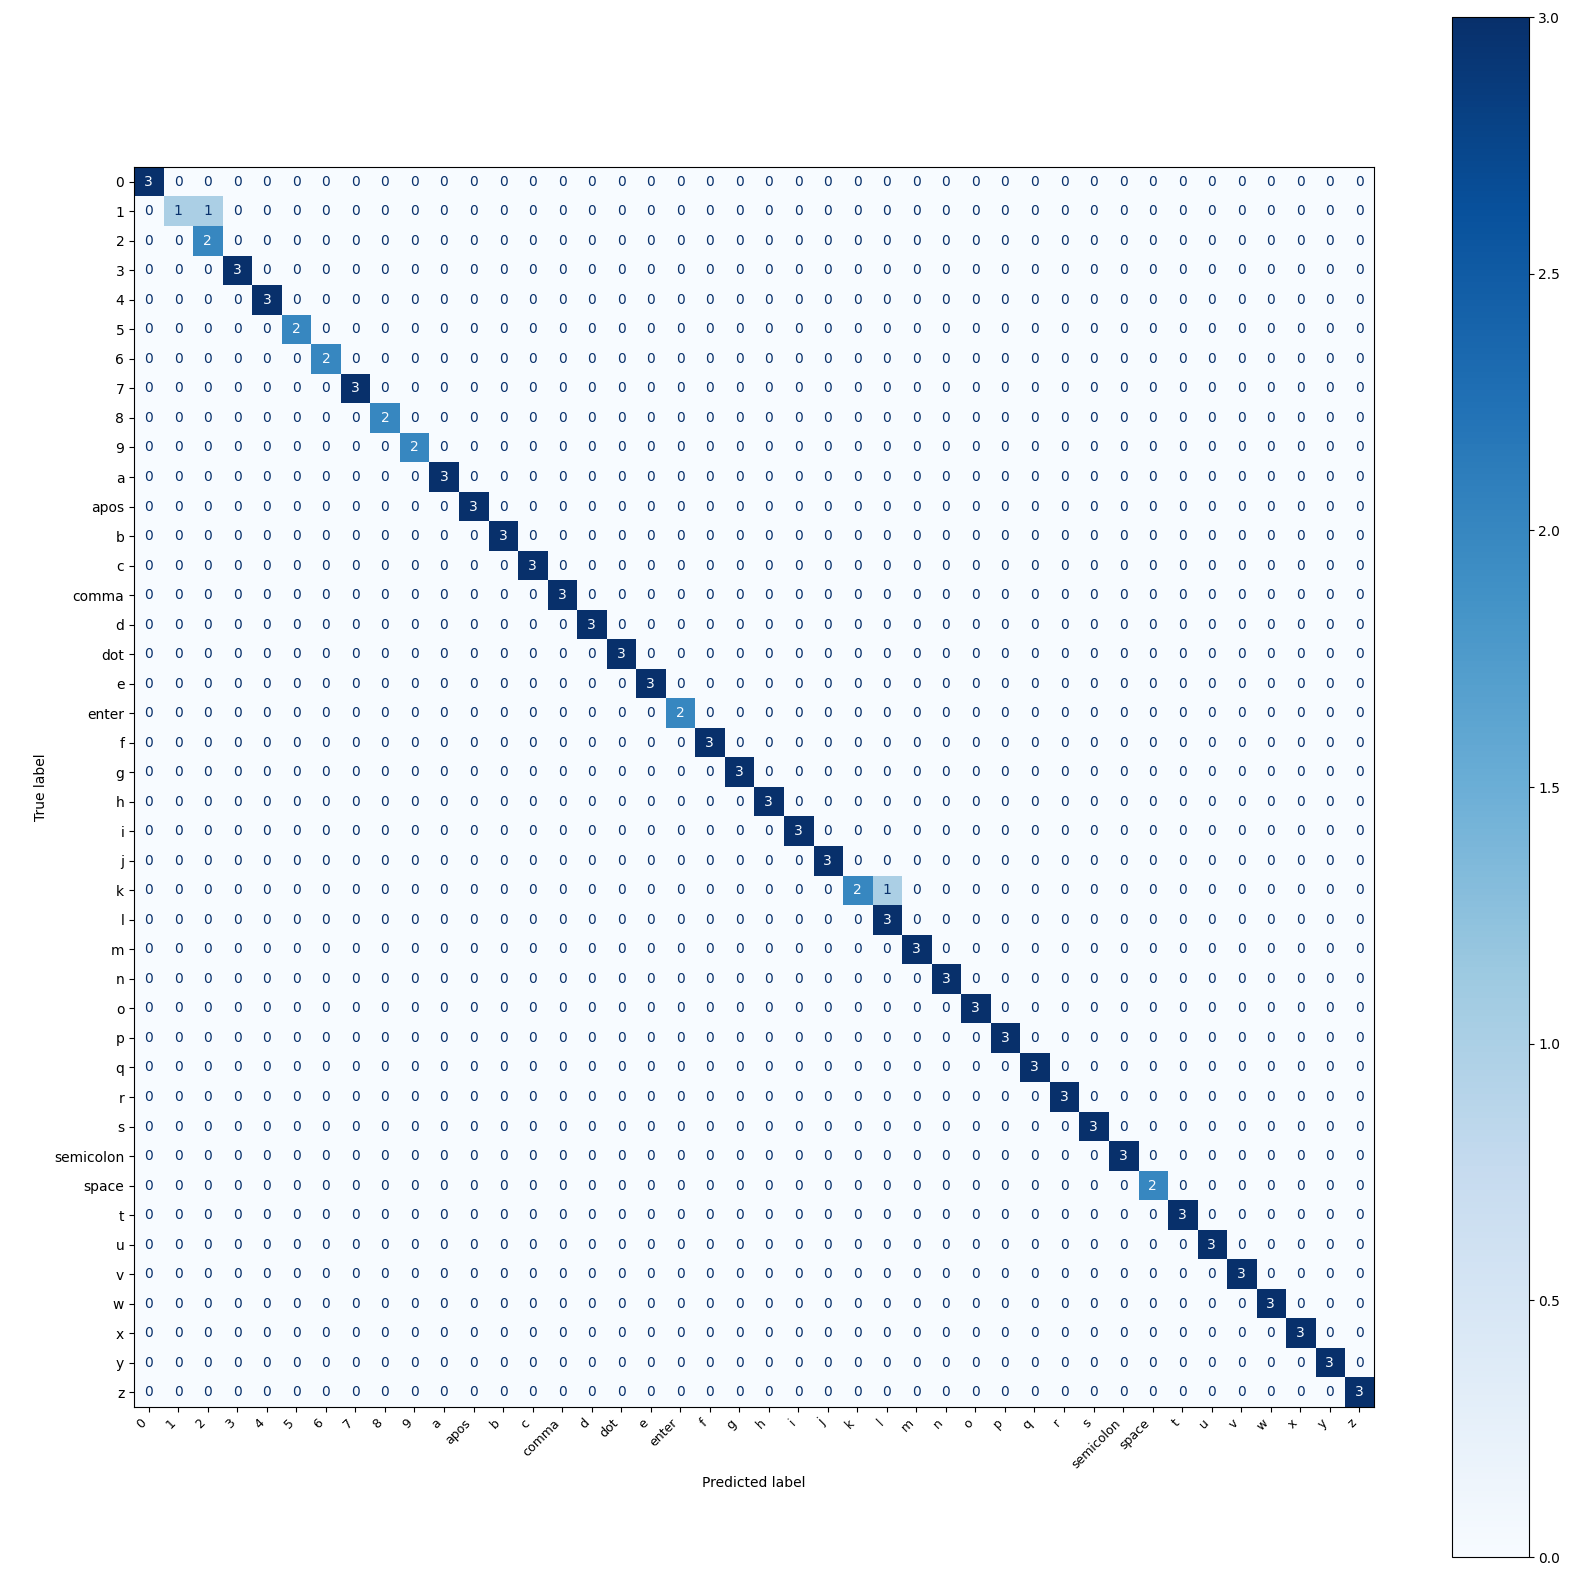
\includegraphics[width=\linewidth]{img_appendix/cm_all_all_n.png}
      \subcaption{Noiseless dataset}
  \end{minipage}
  \hfill
  \begin{minipage}{0.49\linewidth}
      \centering
      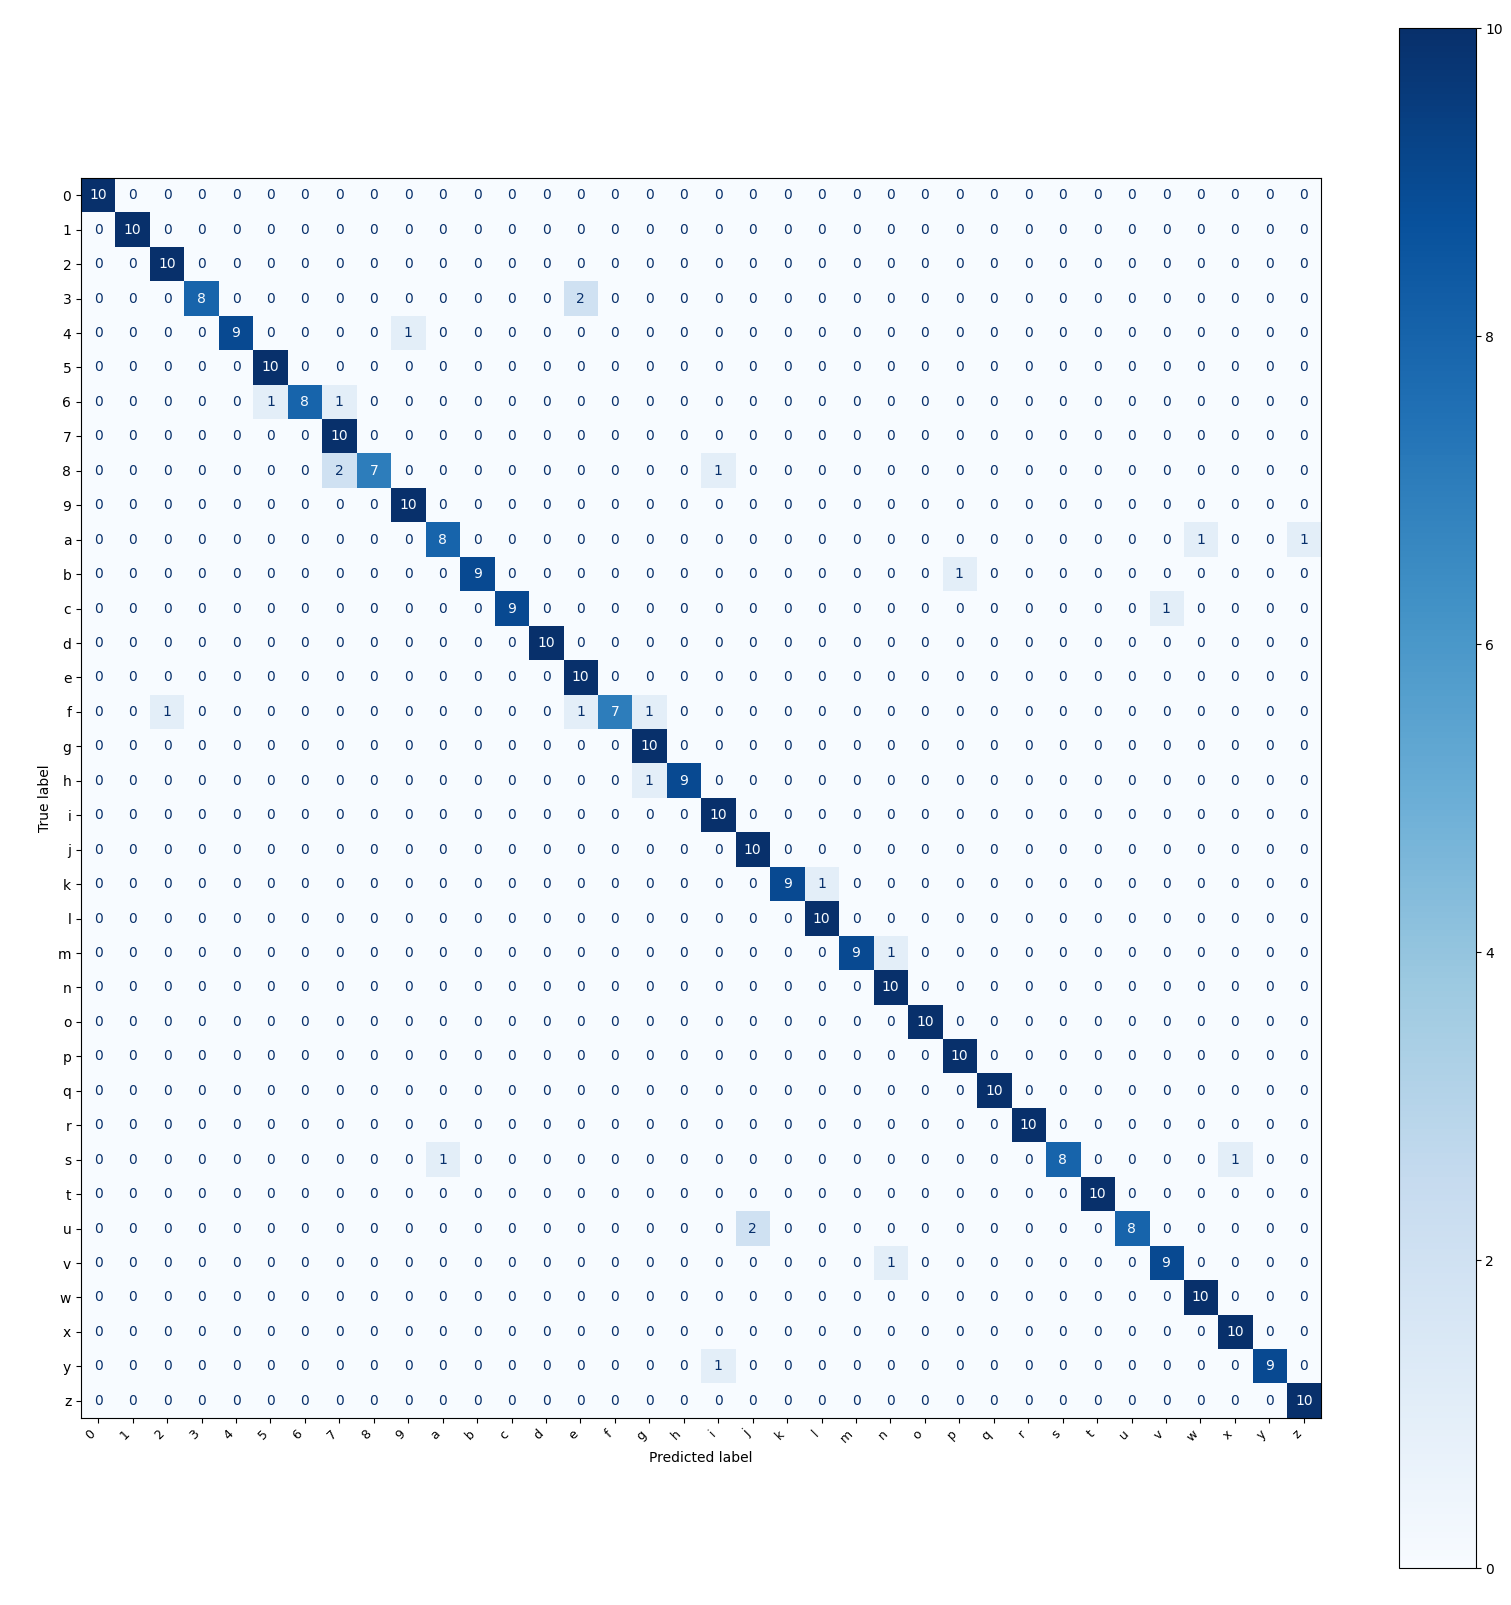
\includegraphics[width=\linewidth]{img_appendix/cm_all_all_p.png}
      \subcaption{Practical dataset}
  \end{minipage}
  \caption{Confusion matrices of the best CoAtNet model using all keys evaluated on few datasets.}
\end{figure}

% \begin{figure}[H]
%   \centering
%     \begin{minipage}{0.49\linewidth}
%       \centering
%       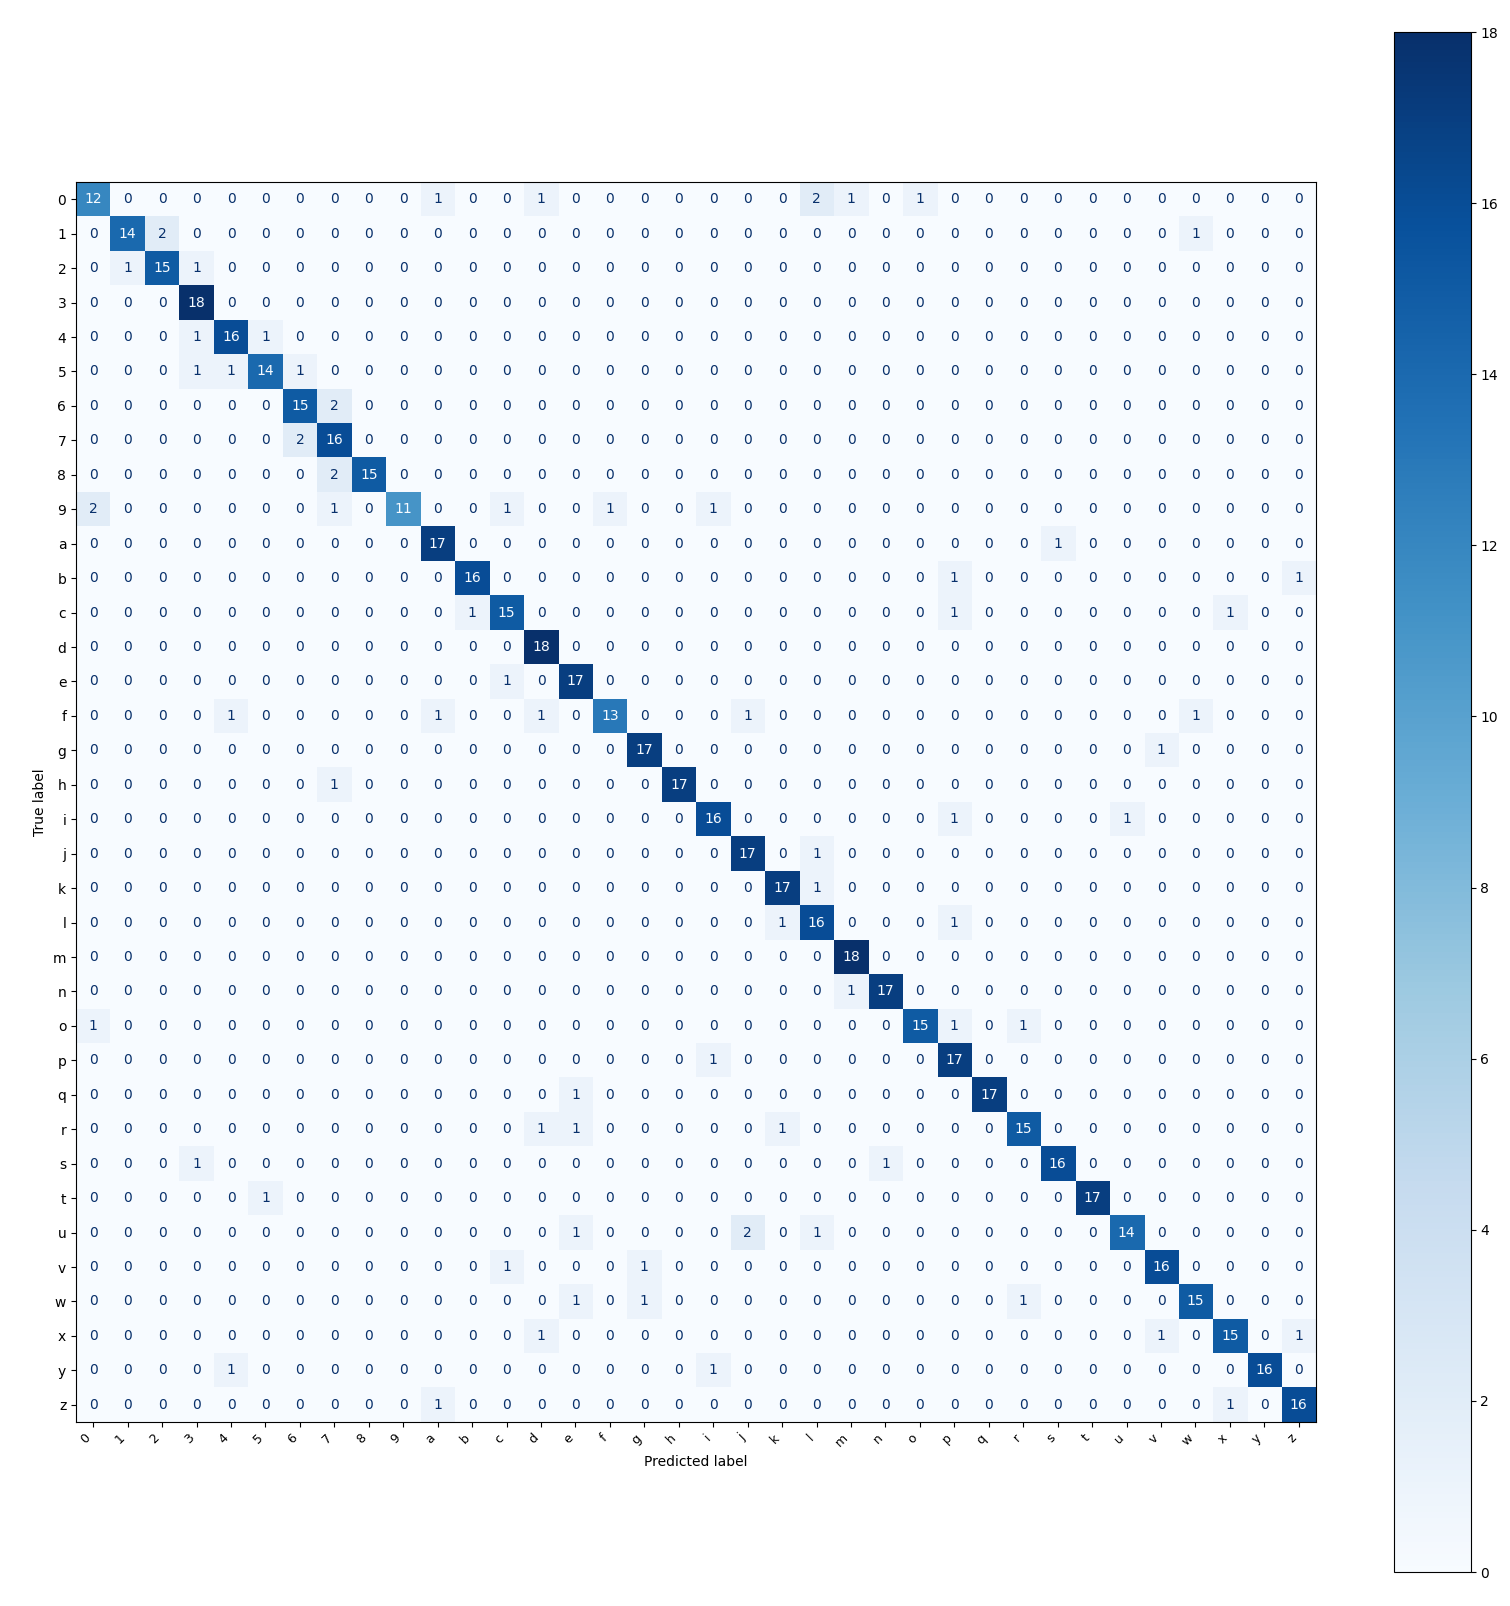
\includegraphics[width=\linewidth]{img_appendix/cm_all_moat_alphanum_all.png}
%       \subcaption{}
%   \end{minipage}
%   \begin{minipage}{0.49\linewidth}
%       \centering
%       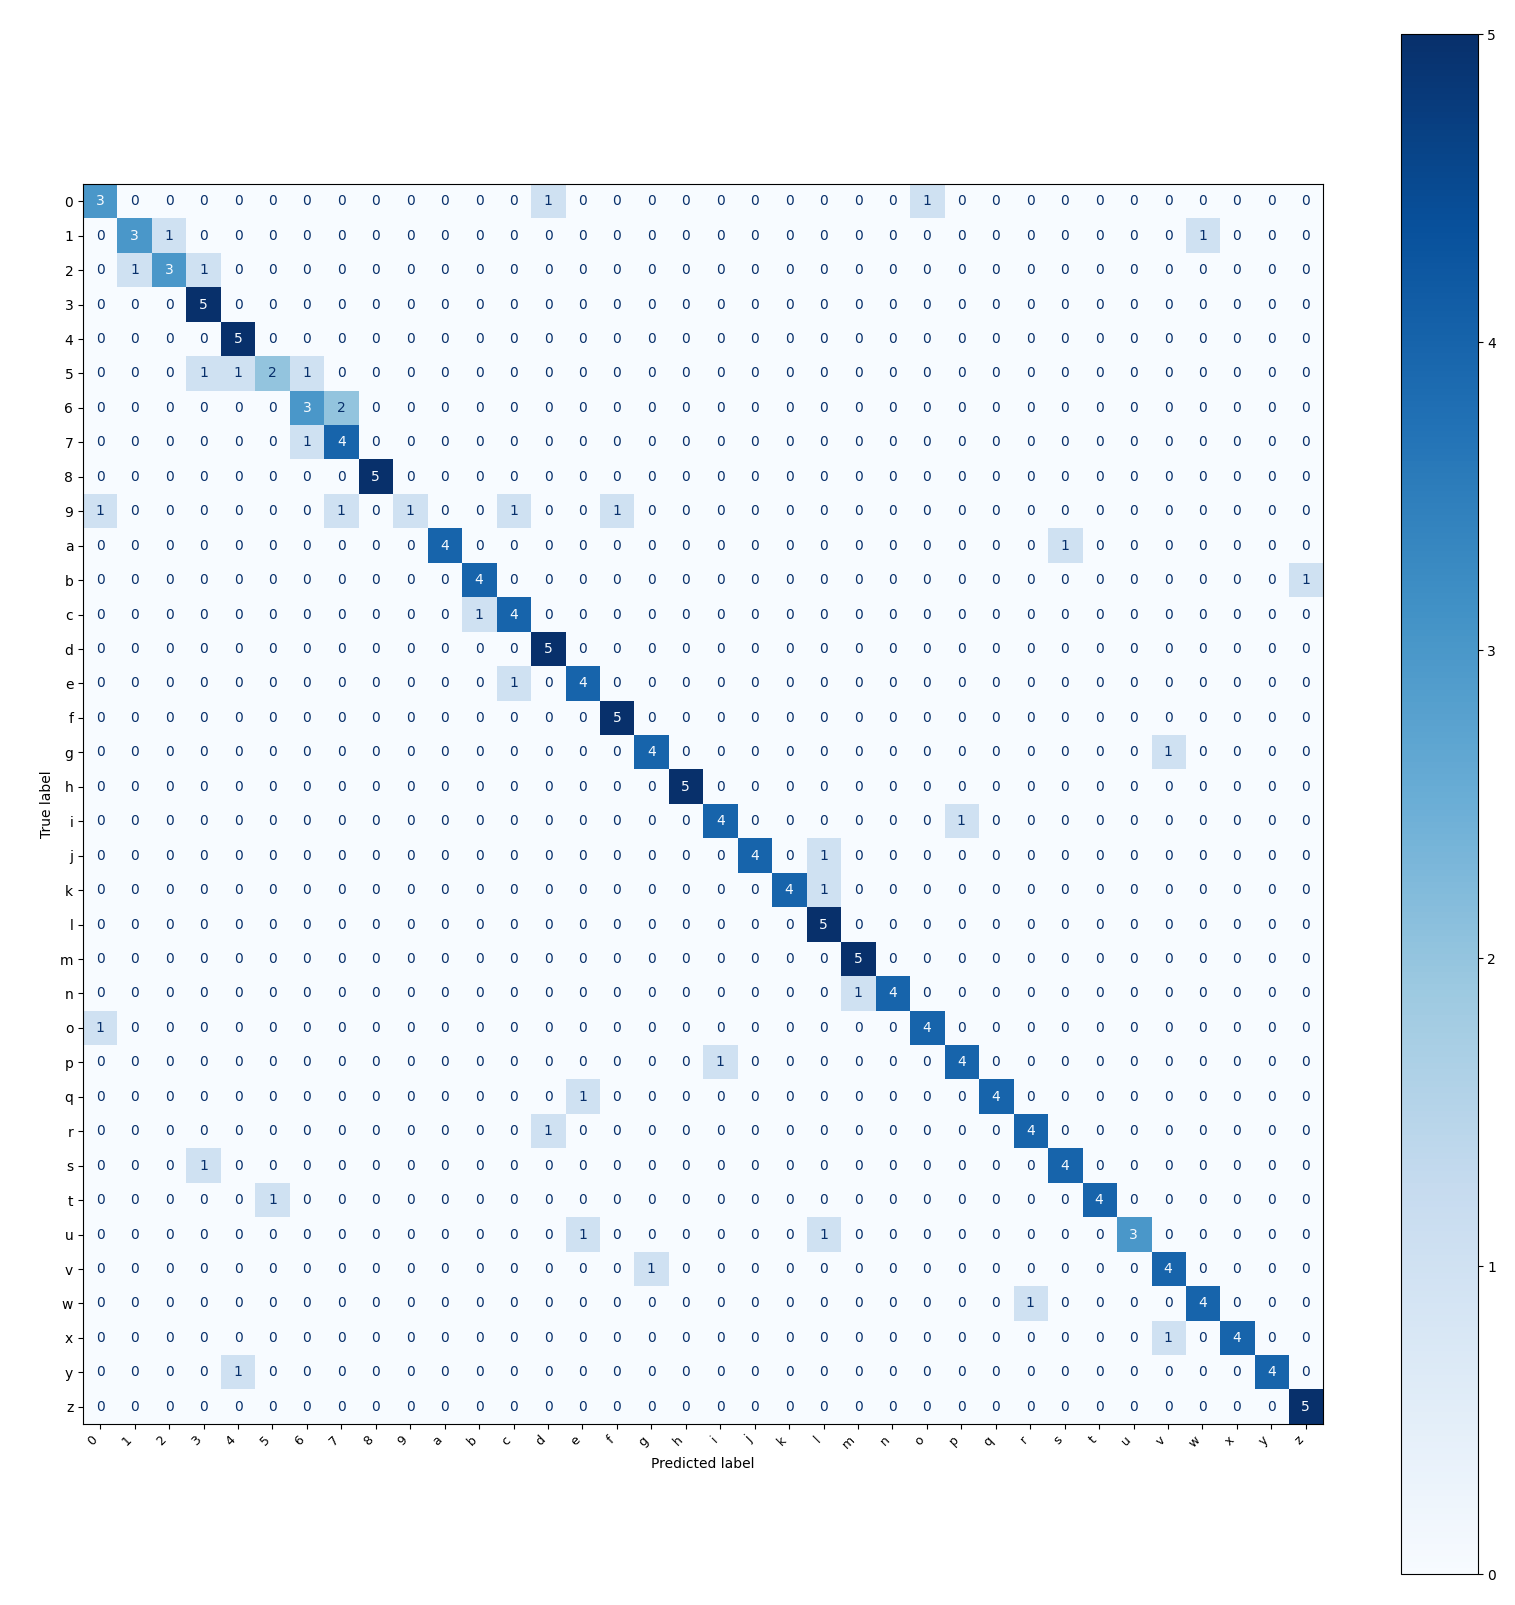
\includegraphics[width=\linewidth]{img_appendix/cm_all_moat_alphanum_mka.png}
%       \subcaption{}
%   \end{minipage}
%   \hfill
%   \begin{minipage}{0.49\linewidth}
%       \centering
%       \includegraphics[width=\linewidth]{img_appendix/cm_all_moat_alphanum_n.png}
%       \subcaption{}
%   \end{minipage}
%   \begin{minipage}{0.49\linewidth}
%       \centering
%       \includegraphics[width=\linewidth]{img_appendix/cm_all_moat_alphanum_p.png}
%       \subcaption{}
%   \end{minipage}
%   \caption{Confusion matrices of the best MOAT model using alphanumeric keys evaluated on: (a) Combined all recordings (b) MKA dataset, (c) Noiseless dataset, (d) Practical dataset.}
% \end{figure}

% \begin{figure}[H]
%   \centering
%     \begin{minipage}{0.49\linewidth}
%       \centering
%       \includegraphics[width=\linewidth]{img_appendix/cm_all_moat_all_all.png}
%       \subcaption{}
%   \end{minipage}
%   \begin{minipage}{0.49\linewidth}
%       \centering
%       \includegraphics[width=\linewidth]{img_appendix/cm_all_moat_all_mka.png}
%       \subcaption{}
%   \end{minipage}
%   \hfill
%   \begin{minipage}{0.49\linewidth}
%       \centering
%       \includegraphics[width=\linewidth]{img_appendix/cm_all_moat_all_n.png}
%       \subcaption{}
%   \end{minipage}
%   \begin{minipage}{0.49\linewidth}
%       \centering
%       \includegraphics[width=\linewidth]{img_appendix/cm_all_moat_all_p.png}
%       \subcaption{}
%   \end{minipage}
%   \caption{Confusion matrices of the best MOAT model using all keys evaluated on: (a) Combined all recordings (b) MKA dataset, (c) Noiseless dataset, (d) Practical dataset.}
% \end{figure}

% \begin{figure}[H]
%   \centering
%     \begin{minipage}{0.49\linewidth}
%       \centering
%       \includegraphics[width=\linewidth]{img_appendix/cm_all_swin_alphanum_all.png}
%       \subcaption{}
%   \end{minipage}
%   \begin{minipage}{0.49\linewidth}
%       \centering
%       \includegraphics[width=\linewidth]{img_appendix/cm_all_swin_alphanum_mka.png}
%       \subcaption{}
%   \end{minipage}
%   \hfill
%   \begin{minipage}{0.49\linewidth}
%       \centering
%       \includegraphics[width=\linewidth]{img_appendix/cm_all_swin_alphanum_n.png}
%       \subcaption{}
%   \end{minipage}
%   \begin{minipage}{0.49\linewidth}
%       \centering
%       \includegraphics[width=\linewidth]{img_appendix/cm_all_swin_alphanum_p.png}
%       \subcaption{}
%   \end{minipage}
%   \caption{Confusion matrices of the best Swin Transformer model using alphanumeric keys evaluated on: (a)Combined all recordings (b) MKA dataset, (c) Noiseless dataset, (d) Practical dataset.}
% \end{figure}

% \begin{figure}[H]
%   \centering
%     \begin{minipage}{0.49\linewidth}
%       \centering
%       \includegraphics[width=\linewidth]{img_appendix/cm_all_swin_all_all.png}
%       \subcaption{}
%   \end{minipage}
%   \begin{minipage}{0.49\linewidth}
%       \centering
%       \includegraphics[width=\linewidth]{img_appendix/cm_all_swin_all_mka.png}
%       \subcaption{}
%   \end{minipage}
%   \hfill
%   \begin{minipage}{0.49\linewidth}
%       \centering
%       \includegraphics[width=\linewidth]{img_appendix/cm_all_swin_all_n.png}
%       \subcaption{}
%   \end{minipage}
%   \begin{minipage}{0.49\linewidth}
%       \centering
%       \includegraphics[width=\linewidth]{img_appendix/cm_all_swin_all_p.png}
%       \subcaption{}
%   \end{minipage}
%   \caption{Confusion matrices of the best Swin Transformer model using all keys evaluated on: (a)Combined all recordings (b) MKA dataset, (c) Noiseless dataset, (d) Practical dataset.}
% \end{figure}


\begin{tcolorbox}[colback=white!5,colframe=gray!20,title=Prompt to reconstruct the words using alphanumeric keys,coltitle=black]
You are given a list of keypresses predicted by a model that represent some meaningful words.
Each keypress corresponds to one element in the input array. The list can contain alphanumeric characters.

Although the model predicts most keypresses correctly, there may be occasional errors (wrong letters or numbers).
Your task is to reconstruct the original words, based on the given predictions.

\textbf{Important requirements:}
\begin{itemize}
  \item Fix obvious typing mistakes so the output is a coherent, grammatically correct English text, but without changing the order of the characters.
  \item The total number of input keypresses must exactly match the total number of keypresses required to produce the fixed output.
  \item If you think a key is mistyped, you may replace it in place with the correct one. However, you cannot delete it or add new ones.
\end{itemize}

\textbf{Example:} \\
Input: [ ['h', 'a', 'l', 'k', 'o'], ['w', 'o', 'r', 'l', 'e'] ] \\
Expected output: [ ['h', 'e', 'l', 'l', 'o' ], ['w', 'o', 'r', 'l', 'd'] ] \\
Explanation: 'a' was mismatched with 'e', 'k' was mistaken with 'l' and 'e' was misclassified with 'd'

Process following list of predictions: \{input\_data\}

Return a list of key lists that are most probable, without any extra explanations, code, additional styling, or comments. You MUST NOT include any comments.
\end{tcolorbox}

\begin{tcolorbox}[colback=white!5,colframe=gray!20,title=Prompt to reconstruct the senteces using all keys,coltitle=black]
You are given a list of keypresses predicted by a model that represent a sentence.
Each keypress corresponds to one element in the input array. The list can contain alphanumeric characters and special keys (such as shifts, cmds, alts etc).

Although the model predicts most keypresses correctly, there may be occasional errors (wrong letters, numbers, or special keys).
Your task is to reconstruct the original sentence, based on the given predictions.

\textbf{Important requirements:}
\begin{itemize}
  \item Fix obvious typing mistakes so the output is a coherent, grammatically correct English sentence, but without changing the order of the characters.
  \item The total number of input keypresses must exactly match the total number of keypresses required to produce the fixed output.
  \item If you think a key is mistyped, you may replace it in place with the correct one. However, you cannot delete it or add new ones.
\end{itemize}

\textbf{Example:} \\
Input: ['caps', 'h', 'caps', 'a', 'l', 'l', 'o', 'space', 'b', 'e', 'u', 't', 'k', 'f', 'u', 'l', 'space', 'shift', 'w', 'o', 'r', 'l', 'e', 'shift', '1']\\
Expected output: ['caps', 'h', 'caps', 'e', 'l', 'l', 'o', 'space', 'b', 'e', 'a', 'u', 't', 'i', 'f', 'u', 'l', 'space', 'shift', 'w', 'o', 'r', 'l', 'e', 'shift', '1']\\
Explanation: 'k' was mismatched with 'i' and 'e' was misclassified with 'd', two 'caps' keys make sense as they result in capitalized 'h' and the last keys create '!'

Process the following list of predictions: \{input\_data\}

Return a list of keypresses that are most probable and create a meaningful sentence, provide it without any extra explanations, code, additional styling, or comments.
\end{tcolorbox}


\newpage
\section*{Real-World Simulation}
\label{appendix_real_world}



\begin{table}[h!]
\centering
\caption{Performance of  models on the custom dataset with only alphanumeric keys.}
\begin{adjustbox}{max width=\textwidth}
\begin{tabular}{l|c|c|c|ccccc}
\hline
\textbf{Model} & \textbf{Architecture} & \textbf{Window} & \textbf{Loss} & \multicolumn{5}{c}{\textbf{Accuracy [\%]}} \\
\cline{5-9}
       &   \textbf{No.}  &   \textbf{Size}   &   & \textbf{All} & \textbf{Clean} & \textbf{Window} & \textbf{Dishwasher} & \textbf{Washing Machine}  \\
\hline
MOAT & 3 & - & 0.0062 & \textbf{81.09} & \textbf{95.0} & 69.16 & 82.41 & \textbf{78.70} \\
CoAtNet & 4 & - & 0.0054 & 80.38 & \textbf{95.0} & \textbf{71.96} & \textbf{83.33} & 72.22 \\
MOAT & 3 & 16 & 0.0064 & 78.49 & 89.0 & 68.22 & 82.41 & 75.00 \\
CoAtNet & 3 & - & 0.0075 & 74.70 & 92.0 & 65.42 & 71.30 & 71.30 \\
MOAT & 2 & 16 & 0.0088 & 72.81 & 85.0 & 62.62 & 75.00 & 69.44 \\
CoAtNet & 2 & - & 0.0084 & 72.34 & 88.0 & 61.68 & 71.30 & 69.44 \\
CoAtNet & 1 & - & 0.0084 & 70.45 & 84.0 & 63.55 & 70.37 & 64.81 \\
MOAT & 4 & - & 0.0138 & 69.27 & 84.0 & 62.62 & 71.30 & 60.19 \\
MOAT & 4 & 16 & 0.0129 & 67.61 & 86.0 & 57.01 & 70.37 & 58.33 \\
MOAT & 2 & - & 0.0150 & 52.96 & 66.0 & 48.60 & 48.15 & 50.00 \\
MOAT & 4 & 8 & 0.0416 & 51.30 & 68.0 & 45.79 & 45.37 & 47.22 \\
MOAT & 1 & 8 & 0.0161 & 50.35 & 69.0 & 43.93 & 42.59 & 47.22 \\
MOAT & 1 & - & 0.0271 & 26.24 & 38.0 & 23.36 & 20.37 & 24.07 \\
\hline
\end{tabular}
\end{adjustbox}
\end{table}


\begin{table}[h!]
\centering
\caption{Performance of models on the custom dataset with all keys.}
\begin{adjustbox}{max width=\textwidth}
\begin{tabular}{l|c|c|c|ccccc}
\hline
\textbf{Model} & \textbf{Architecture} & \textbf{Window} & \textbf{Loss} & \multicolumn{5}{c}{\textbf{Accuracy [\%]}} \\
\cline{5-9}
       &   \textbf{No.}  &   \textbf{Size}   &   & \textbf{All} & \textbf{Clean} & \textbf{Window} & \textbf{Dishwasher} & \textbf{Washing Machine}  \\
\hline
MOAT & 4 & 16 & 0.0058 & \textbf{85.68} & 95.86 & 76.47 & 87.77 & \textbf{83.60} \\
MOAT & 3 & - & 0.0061 & 85.40 & 95.86 & 78.07 & 87.23 & 81.48 \\
MOAT & 3 & 16 & 0.0062 & 85.27 & 94.67 & 75.40 & \textbf{88.30} & \textbf{83.60} \\
CoAtNet & 4 & - & 0.0057 & 84.72 & 95.27 & 74.87 & 87.77 & 82.01 \\
CoAtNet & 3 & - & 0.0068 & 84.45 & \textbf{96.45} & 78.07 & 84.04 & 80.42 \\
MOAT & 4 & 8 & 0.0066 & 84.17 & 91.72 & \textbf{78.61} & 86.70 & 80.42 \\
MOAT & 4 & - & 0.0066 & 83.77 & 92.90 & 77.54 & 85.64 & 79.89 \\
MOAT & 2 & 16 & 0.0068 & 82.54 & 91.72 & 75.40 & 83.51 & 80.42 \\
MOAT & 1 & 8 & 0.0046 & 80.49 & 89.35 & 72.73 & 84.04 & 76.72 \\
CoAtNet & 1 & - & 0.0105 & 75.44 & 91.12 & 68.98 & 73.94 & 69.31 \\
CoAtNet & 2 & - & 0.0104 & 74.22 & 87.57 & 65.24 & 76.60 & 68.78 \\
MOAT & 2 & - & 0.0065 & 66.71 & 80.47 & 60.96 & 62.23 & 64.55 \\
MOAT & 1 & - & 0.0080 & 57.71 & 71.01 & 48.13 & 55.32 & 57.67 \\
\hline
\end{tabular}
\end{adjustbox}
\end{table}

\begin{table}[h!]
\centering
\caption{Model's ability to transfer knowledge across different background noise recordings when trained on clean dataset.}
\begin{adjustbox}{max width=\textwidth}
\begin{tabular}{c|c|c|c|cc}
\hline
\textbf{Keys} & \textbf{Model} & \textbf{Architecture} & \textbf{Window} &  \multicolumn{2}{c}{\textbf{Accuracy [\%]}} \\
\cline{5-6}
       & & \textbf{No.}  &   \textbf{Size}   &  \textbf{Clean} & \textbf{Noisy}  \\
\hline
\multirow{8}{*}{Alphanumeric}
  & MOAT    & 3 & -         & 70.00 & 8.36 \\
  % & MOAT    & 3 & 8         & 65.00 & 8.98 \\
  & MOAT    & 4 & -         & 61.00 & 7.74 \\
  % & MOAT    & 4 & 8         & 58.00 & 6.19 \\
  & MOAT    & 2 & -         & 55.00 & 5.88 \\
  % & MOAT    & 4 & 16        & 52.00 & 6.19 \\
  % & MOAT    & 2 & 16        & 51.85 & 5.88 \\
  & CoAtNet & 4 & -         & 50.00 & 4.33 \\
  & CoAtNet & 2 & -         & 48.15 & 4.33 \\
  & CoAtNet & 3 & -         & 47.00 & 4.95 \\
  & MOAT    & 1 & 8         & 45.00 & 5.88 \\
  & CoAtNet & 1 & -         & 43.00 & 6.50 \\
  % & MOAT    & 1 & -         & 38.00 & 6.81 \\
\hline
\multirow{8}{*}{All}
  & MOAT    & 3 & 8         & 87.57 & 13.48 \\
  & CoAtNet & 4 & -         & 86.39 & 12.41 \\
  % & MOAT    & 3 & -         & 86.39 & 10.82 \\
  & CoAtNet & 1 & -         & 81.66 & 9.04 \\
  & CoAtNet & 3 & -         & 77.51 & 11.17 \\
  & MOAT    & 4 & -         & 73.37 & 7.98 \\
  & CoAtNet & 2 & -         & 69.23 & 4.61 \\
  & MOAT    & 2 & 16        & 65.09 & 7.27 \\
  % & MOAT    & 4 & 8         & 63.91 & 6.74 \\
  % & MOAT    & 4 & 16        & 59.17 & 6.38 \\
  % & MOAT    & 2 & -         & 55.62 & 5.32 \\
  & MOAT    & 1 & -         & 54.44 & 4.96 \\
  % & MOAT    & 1 & 8         & 53.85 & 4.79 \\
\hline
\end{tabular}
\end{adjustbox}
\end{table}


\begin{table}[h!]
\centering
\caption{Model's ability to transfer knowledge across different background noise recordings when trained on noisy part of custom data.}
\begin{adjustbox}{max width=\textwidth}
\begin{tabular}{c|c|c|c|cc}
\hline
\textbf{Keys} & \textbf{Model} & \textbf{Architecture} & \textbf{Window} &  \multicolumn{2}{c}{\textbf{Accuracy [\%]}} \\
\cline{5-6}
       & & \textbf{No.}  &   \textbf{Size}   &  \textbf{Clean} & \textbf{Noisy}  \\
\hline
\multirow{8}{*}{Alphanumeric}
& CoAtNet & 4 & - & 63.0 & 72.14 \\
& MOAT & 3 & 16 & 58.0 & 71.83 \\
& MOAT & 2 & 16 & 63.0 & 70.28 \\
& CoAtNet & 1 & - & 39.0 & 65.63 \\
& CoAtNet & 2 & - & 41.0 & 62.85 \\
% & MOAT & 3 & - & 23.0 & 56.97 \\
& MOAT & 4 & 16 & 24.0 & 45.2 \\
% & MOAT & 2 & - & 23.0 & 39.63 \\
& MOAT & 1 & 8 & 20.0 & 36.84 \\
% & MOAT & 4 & 8 & 23.0 & 35.91 \\
% & MOAT & 4 & - & 12.0 & 33.44 \\
& CoAtNet & 3 & - & 18.0 & 27.86 \\
% & MOAT & 1 & - & 13.0 & 25.39 \\
\hline
\multirow{8}{*}{All}
& CoAtNet & 4 & - & 71.01 & 78.72 \\
& MOAT & 4 & 16 & 66.27 & 78.19 \\
& MOAT & 3 & - & 67.46 & 78.01 \\
& CoAtNet & 3 & - & 72.78 & 77.30 \\
% & MOAT & 4 & 8 & 65.68 & 76.60 \\
% & MOAT & 3 & 16 & 57.99 & 75.35 \\
& MOAT & 2 & 16 & 57.40 & 75.18 \\
& CoAtNet & 2 & - & 45.56 & 67.91 \\
& CoAtNet & 1 & - & 38.46 & 64.36 \\
% & MOAT & 2 & - & 36.69 & 57.98 \\
& MOAT & 1 & 8 & 23.08 & 50.89 \\
% & MOAT & 1 & - & 27.22 & 44.33 \\
% & MOAT & 4 & - & 20.71 & 37.94 \\
\hline
\end{tabular}
\end{adjustbox}
\end{table}



% \begin{table}[h!]
% \centering
% \caption{Performance of  models on the \textbf{alphanumeric} ... dataset.}
% \begin{adjustbox}{max width=\textwidth}
% \begin{tabular}{l|c|c|c|c|cc}
% \hline
% \textbf{Approach} & \textbf{Model} & \textbf{Architecture} & \textbf{Window} & \multicolumn{2}{c}{\textbf{Accuracy [\%]}} \\
% \cline{5-6}
%        & &   \textbf{No.}  &   \textbf{Size}   &  \textbf{Clean} & \textbf{Noisy}  \\
% \hline
% Clean $\rightarrow$ Noisy & &  &  &  &  \\
% Clean $\rightarrow$ Noisy & &  &  &  &  \\
% Clean $\rightarrow$ Noisy & &  &  &  &  \\
% Clean $\rightarrow$ Noisy & &  &  &  &  \\
% Clean $\rightarrow$ Noisy & &  &  &  &  \\
% Clean $\rightarrow$ Noisy & &  &  &  &  \\
% Clean $\rightarrow$ Noisy & &  &  &  &  \\
% Clean $\rightarrow$ Noisy & &  &  &  &  \\
% Clean $\rightarrow$ Noisy & &  &  &  &  \\
% Clean $\rightarrow$ Noisy & &  &  &  &  \\
% Clean $\rightarrow$ Noisy & &  &  &  &  \\
% Clean $\rightarrow$ Noisy & &  &  &  &  \\

% % Noisy $\rightarrow$ Clean & &  &  &  &  \\
% % Noisy $\rightarrow$ Clean & &  &  &  &  \\
% % Noisy $\rightarrow$ Clean & &  &  &  &  \\
% % Noisy $\rightarrow$ Clean & &  &  &  &  \\
% % Noisy $\rightarrow$ Clean & &  &  &  &  \\
% % Noisy $\rightarrow$ Clean & &  &  &  &  \\
% % Noisy $\rightarrow$ Clean & &  &  &  &  \\
% % Noisy $\rightarrow$ Clean & &  &  &  &  \\
% % Noisy $\rightarrow$ Clean & &  &  &  &  \\
% % Noisy $\rightarrow$ Clean & &  &  &  &  \\
% % Noisy $\rightarrow$ Clean & &  &  &  &  \\
% % Noisy $\rightarrow$ Clean & &  &  &  &  \\
% \hline
% \end{tabular}
% \end{adjustbox}
% \end{table}


\end{document}


